\section{Arrangements attaining the conjectured bound}\label{app:figures}

This appendix collects the arrangements referred to in the main text, in increasing order of $n$.
The optimal arrangements for $n=6,10,12$ (\cref{fig:n6-all,fig:n10,fig:n10-all,fig:n12-all}) give the lower bounds of \cref{thm:small-n}; the two non-stretchable optima for $n=10$ are drawn with pseudolines (\cref{fig:n10-nonstretchable}).
\Cref{fig:n26} shows the member $\mathcal C_2$ of the series of \cref{thm:series}.
Augmentation (\cref{sec:augment}) gives the arrangements of 20, 32 and 44 pseudolines in \cref{fig:n20,fig:n20-collapse,fig:n32,fig:n44}.
Doubling the arrangement of \cref{fig:n20-collapse} gives the pseudoline series $18\cdot2^t+2$ discussed in \cref{sec:discussion}, whose members with $n=38,74$ are stretchable (\cref{fig:n38,tab:n74-lines}), and doubling that of \cref{fig:n32} gives the series $30\cdot2^t+2$.
\Cref{tab:n20-collapse-lines,tab:n32-lines,tab:n38-lines,tab:n74-lines} give the equations of the stretched arrangements.

Different shades correspond to different phases of the local coloring (\cref{fig:phase-seam}); unbounded triangles are lighter.
The boundaries between the phases are thus the unused and double segments, that is, the part of the phase seam (\cref{def:seam}) visible in the affine chart.
\Cref{fig:n44} is not colored.

The coefficients $m_i,b_i$ in the tables are exact.
We checked in rational arithmetic that for these values the triple points are exact, the order of the crossings on every line agrees with the word of the arrangement, and the number of triangles is as stated.

For brevity, letters in the words are written as their initial slot followed by $m-2$ asterisks: a simple crossing $(g,2)\mapsto g$, a triple point $(g,3)\mapsto g*$, a crossing of multiplicity 4 $(g,4)\mapsto g**$, and so on.


\newcommand\ngap{\hspace{0.01\linewidth}}
% Grid cell for n=6: 3 pictures of 0.326 and 2 gaps of 0.01 of the line width
% (the sum must not exceed 1, otherwise the last picture wraps to the next line).
\newcommand\nsix[1]{\begin{minipage}{0.326\linewidth}\input{figures/n6/6-#1}\end{minipage}}

\begin{figure}[t]
\centering
\nsix{1330sgdjqf8p8}\ngap\nsix{1nevwww2r41us}\ngap\nsix{3asa5zegavnkz}\par\vspace{1mm}
\nsix{3pkh1zclcef98}\ngap\nsix{2d5kqooycn0g3}\ngap\nsix{3aiagxuwsbcdh}
\caption{All 6 optimal arrangements for $n=6$ ($a_3=7$), with $t_3=0,0,1$ in the first row and $t_3=2,3,3$ in the second.}
\label{fig:n6-all}
\end{figure}

\begin{figure}[p]
\centering
% Both figures have the same picture height, 0.685 of the line width (the largest that fits
% the page together with the caption); the gap between pictures is as in the grids.
\begin{minipage}{0.685\linewidth}% Generated by svg2tikz.py from 27.svg
\begin{tikzpicture}[x=\linewidth,y=\linewidth]
\useasboundingbox (0,0) rectangle (1,1);
\clip (0,0) rectangle (1,1);
\fill[g-b-ext-s3](-0.0760,0.7130)--(-0.0760,0.7320)--(0.0200,0.6846)--cycle;
\fill[g-b-ext-s3](-0.0760,0.9684)--(-0.0760,1.0760)--(0.1530,1.0760)--(0.4719,0.5751)--cycle;
\fill[g-b-ext-s3](0.6259,1.0760)--(0.6904,1.0760)--(0.6052,0.7895)--cycle;
\fill[g-b-ext-s3](0.8368,1.0760)--(0.9438,1.0760)--(0.6936,0.7829)--cycle;
\fill[g-w](0.6904,1.0760)--(0.8368,1.0760)--(0.6936,0.7829)--(0.5964,0.6690)--(0.6052,0.7895)--cycle;
\fill[g-b-int-s3](0.6052,0.7895)--(0.5964,0.6690)--(0.5548,0.6202)--cycle;
\fill[g-w](0.1530,1.0760)--(0.6259,1.0760)--(0.6052,0.7895)--(0.5548,0.6202)--(0.4994,0.5554)--(0.4719,0.5751)--cycle;
\fill[g-w](-0.0760,0.7320)--(-0.0760,0.9684)--(0.4719,0.5751)--(0.4909,0.5454)--(0.0200,0.6846)--cycle;
\fill[g-b-int-s3](0.4719,0.5751)--(0.4994,0.5554)--(0.4909,0.5454)--cycle;
\fill[g-int-s3-w](0.4994,0.5554)--(0.5291,0.5341)--(0.4909,0.5454)--cycle;
\fill[g-b-int-s3](0.5548,0.6202)--(0.5291,0.5341)--(0.4994,0.5554)--cycle;
\fill[g-b-int-s3](0.6936,0.7829)--(0.5892,0.5692)--(0.5964,0.6690)--cycle;
\fill[g-w](0.5964,0.6690)--(0.5892,0.5692)--(0.5666,0.5230)--(0.5291,0.5341)--(0.5548,0.6202)--cycle;
\fill[g-b-ext-s3](1.0760,0.7915)--(1.0760,0.6403)--(0.6468,0.5328)--cycle;
\fill[g-b-int-s3](0.5892,0.5692)--(0.5854,0.5174)--(0.5666,0.5230)--cycle;
\fill[g-w](0.9438,1.0760)--(1.0760,1.0760)--(1.0760,0.7915)--(0.6468,0.5328)--(0.5854,0.5174)--(0.5892,0.5692)--(0.6936,0.7829)--cycle;
\fill[g-b-int-s3](0.5291,0.5341)--(0.5666,0.5230)--(0.5609,0.5113)--cycle;
\fill[g-int-s3-w](0.5666,0.5230)--(0.5854,0.5174)--(0.5609,0.5113)--cycle;
\fill[g-b-int-s3](0.4909,0.5454)--(0.5291,0.5341)--(0.5192,0.5009)--cycle;
\fill[g-int-s3-w](0.5291,0.5341)--(0.5609,0.5113)--(0.5192,0.5009)--cycle;
\fill[g-b-int-s3](0.0200,0.6846)--(0.4909,0.5454)--(0.4348,0.4797)--cycle;
\fill[g-int-s3-w](0.4909,0.5454)--(0.5192,0.5009)--(0.4348,0.4797)--cycle;
\fill[g-b-int-s3](0.6468,0.5328)--(0.6095,0.5103)--(0.5854,0.5174)--cycle;
\fill[g-b-int-s3](0.5854,0.5174)--(0.5838,0.4948)--(0.5609,0.5113)--cycle;
\fill[g-int-s3-w](0.5854,0.5174)--(0.6095,0.5103)--(0.5838,0.4948)--cycle;
\fill[g-b-int-s3](0.5609,0.5113)--(0.5399,0.4684)--(0.5192,0.5009)--cycle;
\fill[g-int-s3-w](0.5609,0.5113)--(0.5838,0.4948)--(0.5399,0.4684)--cycle;
\fill[g-b-int-s3](0.5192,0.5009)--(0.5029,0.4461)--(0.4348,0.4797)--cycle;
\fill[g-int-s3-w](0.5192,0.5009)--(0.5399,0.4684)--(0.5029,0.4461)--cycle;
\fill[g-int-s3-w](0.4348,0.4797)--(0.5029,0.4461)--(0.3034,0.3258)--cycle;
\fill[g-b-int-s3](0.5399,0.4684)--(0.5239,0.4357)--(0.5029,0.4461)--cycle;
\fill[g-int-s3-w](0.5029,0.4461)--(0.5239,0.4357)--(0.4623,0.3095)--cycle;
\fill[g-int-s3-w](0.5399,0.4684)--(0.5776,0.4092)--(0.5239,0.4357)--cycle;
\fill[g-b-int-s3](0.5838,0.4948)--(0.5776,0.4092)--(0.5399,0.4684)--cycle;
\fill[g-int-s3-w](0.5838,0.4948)--(0.9800,0.2105)--(0.5776,0.4092)--cycle;
\fill[g-s4-w](-0.0760,0.3518)--(-0.0760,0.7130)--(0.0200,0.6846)--(0.4348,0.4797)--cycle;
\fill[g-b-ext-s4](-0.0760,0.0971)--(-0.0760,0.3518)--(0.4348,0.4797)--(0.3034,0.3258)--cycle;
\fill[g-ext-s3-w](-0.0396,-0.0760)--(-0.0760,-0.0760)--(-0.0760,0.0971)--(0.3034,0.3258)--cycle;
\fill[g-b-ext](0.2739,-0.0760)--(-0.0396,-0.0760)--(0.3034,0.3258)--(0.5029,0.4461)--(0.4623,0.3095)--cycle;
\fill[g-ext-s3-w](0.3475,-0.0760)--(0.2739,-0.0760)--(0.4623,0.3095)--cycle;
\fill[g-b-ext](0.5425,-0.0760)--(0.3475,-0.0760)--(0.4623,0.3095)--(0.5239,0.4357)--(0.5776,0.4092)--cycle;
\fill[g-ext-s3-w](0.8866,-0.0760)--(0.5425,-0.0760)--(0.5776,0.4092)--cycle;
\fill[g-b-ext-s4](1.0760,0.1415)--(1.0760,-0.0760)--(0.8866,-0.0760)--(0.5776,0.4092)--(0.9800,0.2105)--cycle;
\fill[g-ext-s3-w](1.0760,0.1630)--(1.0760,0.1415)--(0.9800,0.2105)--cycle;
\fill[g-b-ext](1.0760,0.3724)--(1.0760,0.1630)--(0.9800,0.2105)--(0.5838,0.4948)--(0.6095,0.5103)--cycle;
\fill[g-s4-w](1.0760,0.6403)--(1.0760,0.3724)--(0.6095,0.5103)--(0.6468,0.5328)--cycle;
\end{tikzpicture}
\end{minipage}\par\vspace{1mm}
\begin{minipage}{0.685\linewidth}% Generated by svg2tikz.py from 65.svg
\begin{tikzpicture}[x=\linewidth,y=\linewidth]
\useasboundingbox (0,0) rectangle (1,1);
\clip (0,0) rectangle (1,1);
\fill[g-b-ext-s3](-0.0760,0.6955)--(-0.0760,0.7109)--(0.1142,0.6129)--cycle;
\fill[g-b-ext-s3](-0.0760,0.9347)--(-0.0760,1.0760)--(0.0182,1.0760)--(0.3343,0.5843)--cycle;
\fill[g-b-ext-s3](0.1288,1.0760)--(0.2345,1.0760)--(0.3979,0.5761)--cycle;
\fill[g-b-ext-s3](0.9059,1.0760)--(0.9215,1.0760)--(0.8431,0.9800)--cycle;
\fill[g-b-ext-s3](1.0375,1.0760)--(1.0719,1.0760)--(0.8858,0.9154)--cycle;
\fill[g-w](0.9215,1.0760)--(1.0375,1.0760)--(0.8858,0.9154)--(0.6904,0.7467)--(0.8431,0.9800)--cycle;
\fill[g-b-int-s3](0.8431,0.9800)--(0.6904,0.7467)--(0.5622,0.6361)--cycle;
\fill[g-w](0.2345,1.0760)--(0.9059,1.0760)--(0.8431,0.9800)--(0.5622,0.6361)--(0.4279,0.5202)--(0.3979,0.5761)--cycle;
\fill[g-w](0.0182,1.0760)--(0.1288,1.0760)--(0.3979,0.5761)--(0.4187,0.5123)--(0.3343,0.5843)--cycle;
\fill[g-b-int-s3](0.3979,0.5761)--(0.4279,0.5202)--(0.4187,0.5123)--cycle;
\fill[g-w](-0.0760,0.7109)--(-0.0760,0.9347)--(0.3343,0.5843)--(0.3942,0.4911)--(0.1142,0.6129)--cycle;
\fill[g-b-int-s3](0.3343,0.5843)--(0.4187,0.5123)--(0.3942,0.4911)--cycle;
\fill[g-b-int-s3](0.1142,0.6129)--(0.3942,0.4911)--(0.3778,0.4769)--cycle;
\fill[g-int-s3-w](0.4279,0.5202)--(0.4437,0.4909)--(0.4187,0.5123)--cycle;
\fill[g-b-int-s3](0.5622,0.6361)--(0.4437,0.4909)--(0.4279,0.5202)--cycle;
\fill[g-int-s3-w](0.4187,0.5123)--(0.4308,0.4752)--(0.3942,0.4911)--cycle;
\fill[g-b-int-s3](0.4187,0.5123)--(0.4437,0.4909)--(0.4308,0.4752)--cycle;
\fill[g-int-s3-w](0.3942,0.4911)--(0.4161,0.4572)--(0.3778,0.4769)--cycle;
\fill[g-b-int-s3](0.3942,0.4911)--(0.4308,0.4752)--(0.4161,0.4572)--cycle;
\fill[g-b-int-s3](0.8858,0.9154)--(0.6088,0.6221)--(0.6904,0.7467)--cycle;
\fill[g-w](0.6904,0.7467)--(0.6088,0.6221)--(0.4665,0.4714)--(0.4437,0.4909)--(0.5622,0.6361)--cycle;
\fill[g-int-s3-w](0.4437,0.4909)--(0.4587,0.4631)--(0.4308,0.4752)--cycle;
\fill[g-b-int-s3](0.4437,0.4909)--(0.4665,0.4714)--(0.4587,0.4631)--cycle;
\fill[g-int-s3-w](0.4308,0.4752)--(0.4409,0.4443)--(0.4161,0.4572)--cycle;
\fill[g-b-int-s3](0.4308,0.4752)--(0.4587,0.4631)--(0.4409,0.4443)--cycle;
\fill[g-b-int-s3](0.4161,0.4572)--(0.4409,0.4443)--(0.4310,0.4339)--cycle;
\fill[g-int-s3-w](0.4161,0.4572)--(0.4310,0.4339)--(0.1800,0.1681)--cycle;
\fill[g-int-s3-w](0.4665,0.4714)--(0.4945,0.4475)--(0.4587,0.4631)--cycle;
\fill[g-b-int-s3](0.6088,0.6221)--(0.4945,0.4475)--(0.4665,0.4714)--cycle;
\fill[g-int-s3-w](0.4587,0.4631)--(0.4795,0.4245)--(0.4409,0.4443)--cycle;
\fill[g-b-int-s3](0.4587,0.4631)--(0.4945,0.4475)--(0.4795,0.4245)--cycle;
\fill[g-int-s3-w](0.4409,0.4443)--(0.4581,0.3918)--(0.4310,0.4339)--cycle;
\fill[g-b-int-s3](0.4409,0.4443)--(0.4795,0.4245)--(0.4581,0.3918)--cycle;
\fill[g-int-s3-w](0.4795,0.4245)--(0.6971,0.0200)--(0.4581,0.3918)--cycle;
\fill[g-int-s3-w](0.4945,0.4475)--(0.5858,0.3696)--(0.4795,0.4245)--cycle;
\fill[g-s4-w](-0.0760,0.0852)--(-0.0760,0.6955)--(0.1142,0.6129)--(0.3778,0.4769)--cycle;
\fill[g-b-ext](-0.0505,-0.0760)--(-0.0760,-0.0760)--(-0.0760,0.0852)--(0.3778,0.4769)--(0.4161,0.4572)--(0.1800,0.1681)--cycle;
\fill[g-ext-s3-w](-0.0193,-0.0760)--(-0.0505,-0.0760)--(0.1800,0.1681)--cycle;
\fill[g-b-ext](0.1519,-0.0760)--(-0.0193,-0.0760)--(0.1800,0.1681)--(0.4310,0.4339)--(0.4581,0.3918)--cycle;
\fill[g-ext-s3-w](0.6110,-0.0760)--(0.1519,-0.0760)--(0.4581,0.3918)--cycle;
\fill[g-b-ext-s4](0.7488,-0.0760)--(0.6110,-0.0760)--(0.4581,0.3918)--(0.6971,0.0200)--cycle;
\fill[g-ext-s3-w](0.7588,-0.0760)--(0.7488,-0.0760)--(0.6971,0.0200)--cycle;
\fill[g-b-ext](1.0760,-0.0489)--(1.0760,-0.0760)--(0.7588,-0.0760)--(0.6971,0.0200)--(0.4795,0.4245)--(0.5858,0.3696)--cycle;
\fill[g-ext-s3-w](1.0760,0.1168)--(1.0760,-0.0489)--(0.5858,0.3696)--cycle;
\fill[g-b-ext-s4](1.0760,0.1948)--(1.0760,0.1168)--(0.5858,0.3696)--(0.4945,0.4475)--cycle;
\fill[g-w](1.0719,1.0760)--(1.0760,1.0760)--(1.0760,0.1948)--(0.4945,0.4475)--(0.6088,0.6221)--(0.8858,0.9154)--cycle;
\end{tikzpicture}
\end{minipage}
\caption{Optimal arrangements for $n=10$ with 10 triple points. Top: \texttt{0 2 4 6 5 4 3 1* 3* 6 5 8 6* 4* 2* 0* 8 6* 4* 2* 1 4 3 5* 7}. Bottom: \texttt{0 2 4 6 8 7 6 5 3* 1* 0 5* 3* 1* 8 7 5* 3* 2 1 7* 5* 3* 5 7}.}
\label{fig:n10}
\end{figure}

\begin{figure}[p]
\centering
% Width 0.685/0.87221 of the line width: the same picture height as in fig:n10.
\begin{minipage}{0.785\linewidth}% Generated by va2tikz.py from 10-non-stretchable-1.tex
\begin{tikzpicture}[x=\linewidth,y=\linewidth]
\useasboundingbox (0,-0.87221) rectangle (1,0);
\clip (0,-0.87221) rectangle (1,0);
\fill[g-b-int-s3](0.55709,-0.44700)--(0.49931,-0.49683)--(0.58403,-0.52825)--cycle;
\fill[g-int-s3-w](0.55709,-0.44700)--(0.58403,-0.52825)--(0.62298,-0.45853)--cycle;
\fill[g-b-int-s3](0.55709,-0.44700)--(0.62298,-0.45853)--(0.66277,-0.37379)--cycle;
\fill[g-w](0.55709,-0.44700)--(0.66277,-0.37379)--(0.69551,-0.29990)--(0.60934,-0.31830)--(0.52814,-0.39190)--cycle;
\fill[g-b-int-s3](0.55709,-0.44700)--(0.52814,-0.39190)--(0.49194,-0.42144)--cycle;
\fill[g-int-s3-w](0.55709,-0.44700)--(0.49194,-0.42144)--(0.49931,-0.49683)--cycle;
\fill[g-w](0.66277,-0.37379)--(0.62298,-0.45853)--(1.00000,-0.52192)--(1.00000,-0.24366)--(0.81892,-0.27710)--cycle;
\fill[g-b-int-s3](0.66277,-0.37379)--(0.81892,-0.27710)--(0.69551,-0.29990)--cycle;
\fill[g-ext-s3-w](0.00000,-0.78684)--(0.00000,-0.87221)--(0.05088,-0.87221)--(0.25941,-0.64496)--cycle;
\fill[g-b-ext](0.00000,-0.78684)--(0.25941,-0.64496)--(0.38926,-0.50344)--(0.30969,-0.42072)--(0.00000,-0.49519)--cycle;
\fill[g-b-ext](0.43611,-0.54768)--(0.25941,-0.64496)--(0.05088,-0.87221)--(0.38077,-0.87221)--(0.47003,-0.70401)--cycle;
\fill[g-int-s3-w](0.43611,-0.54768)--(0.47003,-0.70401)--(0.51543,-0.61788)--cycle;
\fill[g-b-int-s3](0.43611,-0.54768)--(0.51543,-0.61788)--(0.49931,-0.49683)--cycle;
\fill[g-int-s3-w](0.43611,-0.54768)--(0.49931,-0.49683)--(0.42490,-0.46933)--cycle;
\fill[g-b-int-s3](0.43611,-0.54768)--(0.42490,-0.46933)--(0.38926,-0.50344)--cycle;
\fill[g-int-s3-w](0.43611,-0.54768)--(0.38926,-0.50344)--(0.25941,-0.64496)--cycle;
\fill[g-s4-w](0.47003,-0.70401)--(0.38077,-0.87221)--(0.49070,-0.87221)--(0.49559,-0.82154)--cycle;
\fill[g-b-int-s3](0.47003,-0.70401)--(0.49559,-0.82154)--(0.51543,-0.61788)--cycle;
\fill[g-b-int-s3](0.58403,-0.52825)--(0.51543,-0.61788)--(0.68441,-0.75712)--cycle;
\fill[g-s4-w](0.58403,-0.52825)--(0.68441,-0.75712)--(0.82347,-0.87221)--(1.00000,-0.87221)--(1.00000,-0.70902)--cycle;
\fill[g-b-ext-s4](0.58403,-0.52825)--(1.00000,-0.70902)--(1.00000,-0.52192)--(0.62298,-0.45853)--cycle;
\fill[g-int-s3-w](0.58403,-0.52825)--(0.49931,-0.49683)--(0.51543,-0.61788)--cycle;
\fill[g-b-ext-s3](0.68441,-0.75712)--(0.73471,-0.87221)--(0.82347,-0.87221)--cycle;
\fill[g-w](0.68441,-0.75712)--(0.51543,-0.61788)--(0.49559,-0.82154)--(0.50662,-0.87221)--(0.73471,-0.87221)--cycle;
\fill[g-b-ext-s3](0.49559,-0.82154)--(0.49070,-0.87221)--(0.50662,-0.87221)--cycle;
\fill[g-w](0.53743,0.00000)--(0.49836,-0.34611)--(0.60934,-0.31830)--(0.74598,-0.18440)--(0.82657,0.00000)--cycle;
\fill[g-b-ext-s4](0.53743,0.00000)--(0.35523,0.00000)--(0.37690,-0.15657)--(0.49836,-0.34611)--cycle;
\fill[g-b-ext-s3](0.82657,0.00000)--(0.74598,-0.18440)--(0.93418,0.00000)--cycle;
\fill[g-b-int-s3](0.49931,-0.49683)--(0.49194,-0.42144)--(0.42490,-0.46933)--cycle;
\fill[g-int-s3-w](0.42490,-0.46933)--(0.49194,-0.42144)--(0.40924,-0.38647)--cycle;
\fill[g-b-int-s3](0.42490,-0.46933)--(0.40924,-0.38647)--(0.30969,-0.42072)--cycle;
\fill[g-int-s3-w](0.42490,-0.46933)--(0.30969,-0.42072)--(0.38926,-0.50344)--cycle;
\fill[g-int-s3-w](0.49194,-0.42144)--(0.52814,-0.39190)--(0.49836,-0.34611)--cycle;
\fill[g-b-int-s3](0.49194,-0.42144)--(0.49836,-0.34611)--(0.40924,-0.38647)--cycle;
\fill[g-int-s3-w](0.30969,-0.42072)--(0.40924,-0.38647)--(0.24179,-0.35347)--cycle;
\fill[g-b-int-s3](0.30969,-0.42072)--(0.24179,-0.35347)--(0.13472,-0.33868)--cycle;
\fill[g-s4-w](0.30969,-0.42072)--(0.13472,-0.33868)--(0.00000,-0.32006)--(0.00000,-0.49519)--cycle;
\fill[g-int-s3-w](0.40924,-0.38647)--(0.49836,-0.34611)--(0.37690,-0.15657)--cycle;
\fill[g-b-ext](0.40924,-0.38647)--(0.37690,-0.15657)--(0.27620,0.00000)--(0.00000,0.00000)--(0.00000,-0.11527)--(0.24179,-0.35347)--cycle;
\fill[g-w](0.69551,-0.29990)--(0.81892,-0.27710)--(1.00000,-0.16499)--(1.00000,0.00000)--(0.93418,0.00000)--(0.74598,-0.18440)--cycle;
\fill[g-b-int-s3](0.69551,-0.29990)--(0.74598,-0.18440)--(0.60934,-0.31830)--cycle;
\fill[g-b-int-s3](0.49836,-0.34611)--(0.52814,-0.39190)--(0.60934,-0.31830)--cycle;
\fill[g-b-ext-s3](0.00000,-0.32006)--(0.13472,-0.33868)--(0.00000,-0.27534)--cycle;
\fill[g-s4-w](0.13472,-0.33868)--(0.24179,-0.35347)--(0.00000,-0.11527)--(0.00000,-0.27534)--cycle;
\fill[g-b-ext-s3](0.81892,-0.27710)--(1.00000,-0.24366)--(1.00000,-0.16499)--cycle;
\fill[g-ext-s3-w](0.37690,-0.15657)--(0.35523,0.00000)--(0.27620,0.00000)--cycle;
\end{tikzpicture}
\end{minipage}\par\vspace{1mm}
\begin{minipage}{0.785\linewidth}% Generated by va2tikz.py from 10-non-stretchable-2.tex
\begin{tikzpicture}[x=\linewidth,y=\linewidth]
\useasboundingbox (0,-0.87221) rectangle (1,0);
\clip (0,-0.87221) rectangle (1,0);
\fill[g-b-ext-s3](0.96608,-0.87221)--(1.00000,-0.87221)--(1.00000,-0.76024)--(0.80787,-0.67375)--cycle;
\fill[g-s4-w](0.96608,-0.87221)--(0.80787,-0.67375)--(0.60439,-0.58274)--(0.74705,-0.87221)--cycle;
\fill[g-s4-w](1.00000,-0.76024)--(1.00000,-0.52700)--(0.64427,-0.46778)--(0.80787,-0.67375)--cycle;
\fill[g-b-int-s3](0.36259,-0.04857)--(0.38118,-0.19097)--(0.48016,-0.28749)--cycle;
\fill[g-w](0.36259,-0.04857)--(0.48016,-0.28749)--(0.59716,-0.22764)--(0.70740,-0.04319)--(0.71332,0.00000)--(0.35625,0.00000)--cycle;
\fill[g-b-ext-s3](0.36259,-0.04857)--(0.35625,0.00000)--(0.33874,0.00000)--cycle;
\fill[g-s4-w](0.36259,-0.04857)--(0.33874,0.00000)--(0.18453,0.00000)--(0.38118,-0.19097)--cycle;
\fill[g-b-int-s3](0.48016,-0.28749)--(0.40907,-0.34368)--(0.50419,-0.36714)--cycle;
\fill[g-int-s3-w](0.48016,-0.28749)--(0.50419,-0.36714)--(0.53138,-0.32937)--cycle;
\fill[g-b-int-s3](0.48016,-0.28749)--(0.53138,-0.32937)--(0.59716,-0.22764)--cycle;
\fill[g-int-s3-w](0.48016,-0.28749)--(0.38118,-0.19097)--(0.40907,-0.34368)--cycle;
\fill[g-b-ext](0.00000,-0.57215)--(0.00000,-0.87221)--(0.11366,-0.87221)--(0.32210,-0.67597)--(0.41864,-0.48765)--(0.30547,-0.40890)--cycle;
\fill[g-s4-w](0.00000,-0.57215)--(0.30547,-0.40890)--(0.08038,-0.36374)--(0.00000,-0.37287)--cycle;
\fill[g-b-ext-s4](1.00000,-0.52700)--(1.00000,-0.34963)--(0.66366,-0.37629)--(0.64427,-0.46778)--cycle;
\fill[g-ext-s3-w](0.32210,-0.67597)--(0.11366,-0.87221)--(0.22149,-0.87221)--cycle;
\fill[g-b-ext](0.32210,-0.67597)--(0.22149,-0.87221)--(0.52860,-0.87221)--(0.54798,-0.79875)--(0.48114,-0.52526)--cycle;
\fill[g-int-s3-w](0.32210,-0.67597)--(0.48114,-0.52526)--(0.41864,-0.48765)--cycle;
\fill[g-b-int-s3](0.53867,-0.45153)--(0.48114,-0.52526)--(0.60439,-0.58274)--cycle;
\fill[g-int-s3-w](0.53867,-0.45153)--(0.60439,-0.58274)--(0.64427,-0.46778)--cycle;
\fill[g-b-int-s3](0.53867,-0.45153)--(0.64427,-0.46778)--(0.58627,-0.38275)--cycle;
\fill[g-int-s3-w](0.53867,-0.45153)--(0.58627,-0.38275)--(0.50419,-0.36714)--cycle;
\fill[g-b-int-s3](0.53867,-0.45153)--(0.50419,-0.36714)--(0.44876,-0.43679)--cycle;
\fill[g-int-s3-w](0.53867,-0.45153)--(0.44876,-0.43679)--(0.48114,-0.52526)--cycle;
\fill[g-b-ext-s4](0.60439,-0.58274)--(0.54798,-0.79875)--(0.56604,-0.87221)--(0.74705,-0.87221)--cycle;
\fill[g-b-int-s3](0.60439,-0.58274)--(0.80787,-0.67375)--(0.64427,-0.46778)--cycle;
\fill[g-int-s3-w](0.60439,-0.58274)--(0.48114,-0.52526)--(0.54798,-0.79875)--cycle;
\fill[g-int-s3-w](0.40907,-0.34368)--(0.20463,-0.34963)--(0.30547,-0.40890)--cycle;
\fill[g-b-int-s3](0.40907,-0.34368)--(0.30547,-0.40890)--(0.44876,-0.43679)--cycle;
\fill[g-int-s3-w](0.40907,-0.34368)--(0.44876,-0.43679)--(0.50419,-0.36714)--cycle;
\fill[g-b-ext](0.40907,-0.34368)--(0.38118,-0.19097)--(0.18453,0.00000)--(0.00000,0.00000)--(0.00000,-0.22874)--(0.20463,-0.34963)--cycle;
\fill[g-b-int-s3](0.50419,-0.36714)--(0.58627,-0.38275)--(0.53138,-0.32937)--cycle;
\fill[g-b-int-s3](0.41864,-0.48765)--(0.48114,-0.52526)--(0.44876,-0.43679)--cycle;
\fill[g-int-s3-w](0.41864,-0.48765)--(0.44876,-0.43679)--(0.30547,-0.40890)--cycle;
\fill[g-w](0.59716,-0.22764)--(0.53138,-0.32937)--(0.58627,-0.38275)--(0.67694,-0.27589)--(0.68804,-0.18431)--cycle;
\fill[g-b-int-s3](0.59716,-0.22764)--(0.68804,-0.18431)--(0.70740,-0.04319)--cycle;
\fill[g-w](0.70740,-0.04319)--(0.68804,-0.18431)--(0.81768,-0.12461)--(0.93359,0.00000)--(0.73321,0.00000)--cycle;
\fill[g-b-ext-s3](0.70740,-0.04319)--(0.73321,0.00000)--(0.71332,0.00000)--cycle;
\fill[g-int-s3-w](0.64427,-0.46778)--(0.66366,-0.37629)--(0.58627,-0.38275)--cycle;
\fill[g-w](0.66366,-0.37629)--(1.00000,-0.34963)--(1.00000,-0.04066)--(0.81768,-0.12461)--(0.67694,-0.27589)--cycle;
\fill[g-b-int-s3](0.66366,-0.37629)--(0.67694,-0.27589)--(0.58627,-0.38275)--cycle;
\fill[g-b-ext-s3](0.00000,-0.37287)--(0.08038,-0.36374)--(0.00000,-0.34769)--cycle;
\fill[g-s4-w](0.00000,-0.34769)--(0.08038,-0.36374)--(0.20463,-0.34963)--(0.00000,-0.22874)--cycle;
\fill[g-b-int-s3](0.67694,-0.27589)--(0.81768,-0.12461)--(0.68804,-0.18431)--cycle;
\fill[g-b-ext-s3](0.81768,-0.12461)--(1.00000,-0.04066)--(1.00000,0.00000)--(0.93359,0.00000)--cycle;
\fill[g-ext-s3-w](0.54798,-0.79875)--(0.52860,-0.87221)--(0.56604,-0.87221)--cycle;
\fill[g-b-int-s3](0.08038,-0.36374)--(0.30547,-0.40890)--(0.20463,-0.34963)--cycle;
\end{tikzpicture}
\end{minipage}
\caption{Non-stretchable optimal arrangements for $n=10$ with 10 triple points, drawn with pseudolines. Top: \texttt{0 1 3 6 7 5* 4 2* 0* 4* 2* 6* 4* 8 6* 5 3* 1* 0 3 4 6 5 4 6}. Bottom: \texttt{0 1 4 3 6 8 7 6 4* 2* 0* 6 4* 2* 1 8 6* 4* 2* 1 8 6* 4* 3 6}.
  Non-stretchability was verified by the method of biquadratic final polynomials~\cite{br90}; the certificates are in the repository~\cite{nonsimple-arrangements}.}
\label{fig:n10-nonstretchable}
\end{figure}

% Grid cell: 5 pictures of 0.192 and 4 gaps of 0.01 of the line width.
\newcommand\nten[1]{\begin{minipage}{0.192\linewidth}\input{figures/n10/#1}\end{minipage}}

\begin{figure}[p]
\noindent\nten{10}\ngap\nten{14}\ngap\nten{15}\ngap\nten{16}\ngap\nten{24}\par\vspace{1mm}
\noindent\nten{25}\ngap\nten{26}\ngap\nten{33}\ngap\nten{37}\ngap\nten{38}\par\vspace{1mm}
\noindent\nten{40}\ngap\nten{41}\ngap\nten{42}\ngap\nten{44}\ngap\nten{45}\par\vspace{1mm}
\noindent\nten{47}\ngap\nten{48}\ngap\nten{49}\ngap\nten{50}\ngap\nten{51}\par\vspace{1mm}
\noindent\nten{52}\ngap\nten{54}\ngap\nten{56}\ngap\nten{57}\ngap\nten{58}\par\vspace{1mm}
\noindent\nten{59}\ngap\nten{60}\ngap\nten{61}\ngap\nten{62}\ngap\nten{63}\par\vspace{1mm}
\noindent\nten{64}\ngap\nten{66}\ngap\nten{67}\ngap\nten{68}\ngap\nten{69}
\caption{Optimal arrangements for $n=10$ ($a_3=25$): the stretchable arrangements other than those in \cref{fig:n10}, in increasing order of the number $t_3$ of triple points. Here $t_3=0$.}
\label{fig:n10-all}
\end{figure}

\begin{figure}[p]
\ContinuedFloat
\noindent\nten{70}\ngap\nten{07}\ngap\nten{17}\ngap\nten{18}\ngap\nten{21}\par\vspace{1mm}
\noindent\nten{23}\ngap\nten{30}\ngap\nten{39}\ngap\nten{55}\ngap\nten{04}\par\vspace{1mm}
\noindent\nten{13}\ngap\nten{22}\ngap\nten{03}\ngap\nten{05}\ngap\nten{12}\par\vspace{1mm}
\noindent\nten{28}\ngap\nten{29}\ngap\nten{02}\ngap\nten{11}\ngap\nten{35}\par\vspace{1mm}
\noindent\nten{01}\ngap\nten{06}\ngap\nten{19}\ngap\nten{53}\ngap\nten{09}\par\vspace{1mm}
\noindent\nten{20}\ngap\nten{34}\ngap\nten{43}\ngap\nten{08}\ngap\nten{36}\par\vspace{1mm}
\noindent\nten{46}\ngap\nten{31}\ngap\nten{32}
\caption[]{(continued) The first picture is the last one with $t_3=0$. It is followed, row by row, by $t_3=1$ (8 arrangements), $2$ (3), $3$ (5), $4$ (3), $5$ (3), $6$ (1), $7$ (4), $8$ (3), $9$ (2).}
\end{figure}

% Grid cell for n=12: 4 pictures of 0.2425 and 3 gaps of 0.01 of the line width.
\newcommand\ntw[1]{\begin{minipage}{0.2425\linewidth}\input{figures/n12/#1}\end{minipage}}

\begin{figure}[p]
\noindent\ntw{05}\ngap\ntw{06}\ngap\ntw{09}\ngap\ntw{13}\par\vspace{1mm}
\noindent\ntw{14}\ngap\ntw{15}\ngap\ntw{17}\ngap\ntw{18}\par\vspace{1mm}
\noindent\ntw{02}\ngap\ntw{08}\ngap\ntw{16}\ngap\ntw{19}\par\vspace{1mm}
\noindent\ntw{01}\ngap\ntw{03}\ngap\ntw{04}\ngap\ntw{11}\par\vspace{1mm}
\noindent\ntw{12}\ngap\ntw{10}\ngap\ntw{07}
\caption{All 19 optimal arrangements for $n=12$ ($a_3=38$) in increasing order of the number of triple points: $t_3=2$ (the first two rows), $3$ (the third row), $4$ (the fourth row and the first picture of the fifth), $5$ and $6$.}
\label{fig:n12-all}
\end{figure}

\begin{figure}[p]
\noindent% Generated by svg2tikz.py from 20-2dlmjzueiap0b.svg
\begin{tikzpicture}[x=\linewidth,y=\linewidth]
\useasboundingbox (0,0) rectangle (1,1.46202);
\clip (0,0) rectangle (1,1.46202);
\fill[g-b-ext-s3](0.7286,1.5731)--(0.7594,1.5731)--(0.6399,1.2112)--cycle;
\fill[g-b-ext-s3](0.9673,1.5731)--(0.9983,1.5731)--(0.8534,1.3280)--cycle;
\fill[g-s4-w](0.9983,1.5731)--(1.0588,1.5731)--(0.8472,1.3146)--(0.8534,1.3280)--cycle;
\fill[g-b-int-s3](0.8534,1.3280)--(0.8472,1.3146)--(0.8411,1.3072)--cycle;
\fill[g-b-ext-s4](1.0588,1.5731)--(1.3421,1.5731)--(1.3421,1.3829)--(0.6699,0.9332)--(0.8472,1.3146)--cycle;
\fill[g-ext-s3-w](1.3421,1.0347)--(1.3421,0.9898)--(0.9800,0.9322)--cycle;
\fill[g-ext-s3-w](1.3421,0.8738)--(1.3421,0.7063)--(0.6895,0.8350)--cycle;
\fill[g-ext-s3-w](1.3421,0.5569)--(1.3421,0.4525)--(0.9130,0.6900)--cycle;
\fill[g-ext-s3-w](1.3421,0.2338)--(1.3421,0.1577)--(0.6966,0.7158)--cycle;
\fill[g-ext-s3-w](1.1940,-0.1111)--(1.1293,-0.1111)--(0.9751,0.1556)--cycle;
\fill[g-ext-s3-w](0.7850,-0.1111)--(0.7521,-0.1111)--(0.7344,0.0830)--cycle;
\fill[g-b-ext](1.1293,-0.1111)--(0.7850,-0.1111)--(0.7344,0.0830)--(0.6968,0.4945)--(0.9751,0.1556)--cycle;
\fill[g-int-s3-w](0.9751,0.1556)--(0.6968,0.4945)--(0.6813,0.6633)--cycle;
\fill[g-b-ext](1.3421,0.1577)--(1.3421,-0.1111)--(1.1940,-0.1111)--(0.9751,0.1556)--(0.6813,0.6633)--(0.6751,0.7318)--(0.6966,0.7158)--cycle;
\fill[g-int-s3-w](0.6966,0.7158)--(0.6751,0.7318)--(0.6748,0.7346)--cycle;
\fill[g-b-ext](1.3421,0.4525)--(1.3421,0.2338)--(0.6966,0.7158)--(0.6748,0.7346)--(0.6721,0.7647)--(0.9130,0.6900)--cycle;
\fill[g-int-s3-w](0.9130,0.6900)--(0.6721,0.7647)--(0.6664,0.8265)--cycle;
\fill[g-b-ext](1.3421,0.7063)--(1.3421,0.5569)--(0.9130,0.6900)--(0.6664,0.8265)--(0.6658,0.8336)--(0.6895,0.8350)--cycle;
\fill[g-int-s3-w](0.6895,0.8350)--(0.6658,0.8336)--(0.6652,0.8398)--cycle;
\fill[g-b-ext](1.3421,0.9898)--(1.3421,0.8738)--(0.6895,0.8350)--(0.6652,0.8398)--(0.6649,0.8431)--(0.9800,0.9322)--cycle;
\fill[g-int-s3-w](0.9800,0.9322)--(0.6649,0.8431)--(0.6614,0.8816)--cycle;
\fill[g-b-ext](1.3421,1.1899)--(1.3421,1.0347)--(0.9800,0.9322)--(0.6614,0.8816)--(0.6610,0.8862)--cycle;
\fill[g-w](1.3421,1.3829)--(1.3421,1.1899)--(0.6610,0.8862)--(0.6589,0.9095)--(0.6699,0.9332)--cycle;
\fill[g-b-int-s3](0.6699,0.9332)--(0.6589,0.9095)--(0.6574,0.9249)--cycle;
\fill[g-w](0.8472,1.3146)--(0.6699,0.9332)--(0.6574,0.9249)--(0.6518,0.9869)--(0.8411,1.3072)--cycle;
\fill[g-b-int-s3](0.8411,1.3072)--(0.6518,0.9869)--(0.6445,1.0670)--cycle;
\fill[g-w](0.7594,1.5731)--(0.9673,1.5731)--(0.8534,1.3280)--(0.8411,1.3072)--(0.6445,1.0670)--(0.6336,1.1857)--(0.6399,1.2112)--cycle;
\fill[g-b-int-s3](0.6399,1.2112)--(0.6336,1.1857)--(0.6332,1.1908)--cycle;
\fill[g-w](0.6193,1.5731)--(0.7286,1.5731)--(0.6399,1.2112)--(0.6332,1.1908)--(0.6111,1.4328)--cycle;
\fill[g-b-int-s3](0.6332,1.1908)--(0.5891,1.0573)--(0.6111,1.4328)--cycle;
\fill[g-b-int-s3](0.6445,1.0670)--(0.5874,0.9974)--(0.6336,1.1857)--cycle;
\fill[g-w](0.6336,1.1857)--(0.5874,0.9974)--(0.5854,0.9949)--(0.5891,1.0573)--(0.6332,1.1908)--cycle;
\fill[g-b-int-s3](0.5891,1.0573)--(0.5854,0.9949)--(0.5570,0.9602)--cycle;
\fill[g-b-int-s3](0.5874,0.9974)--(0.5850,0.9873)--(0.5854,0.9949)--cycle;
\fill[g-b-int-s3](0.6574,0.9249)--(0.5875,0.8780)--(0.6518,0.9869)--cycle;
\fill[g-b-int-s3](0.6610,0.8862)--(0.6446,0.8789)--(0.6589,0.9095)--cycle;
\fill[g-int-s3-w](0.6614,0.8816)--(0.6446,0.8789)--(0.6610,0.8862)--cycle;
\fill[g-int-s3-w](0.6652,0.8398)--(0.6582,0.8412)--(0.6649,0.8431)--cycle;
\fill[g-int-s3-w](0.6664,0.8265)--(0.6547,0.8329)--(0.6658,0.8336)--cycle;
\fill[g-b-int](0.6658,0.8336)--(0.6547,0.8329)--(0.6461,0.8377)--(0.6582,0.8412)--(0.6652,0.8398)--cycle;
\fill[g-b-int](0.6649,0.8431)--(0.6582,0.8412)--(0.6297,0.8468)--(0.6446,0.8789)--(0.6614,0.8816)--cycle;
\fill[g-int-s3-w](0.6582,0.8412)--(0.6461,0.8377)--(0.6297,0.8468)--cycle;
\fill[g-int-s3-w](0.6446,0.8789)--(0.6297,0.8468)--(0.6042,0.8609)--cycle;
\fill[g-b-int-s3](0.6446,0.8789)--(0.6042,0.8609)--(0.5880,0.8699)--cycle;
\fill[g-w](0.6589,0.9095)--(0.6446,0.8789)--(0.5880,0.8699)--(0.5840,0.8721)--(0.5875,0.8780)--(0.6574,0.9249)--cycle;
\fill[g-b-int-s3](0.5875,0.8780)--(0.5840,0.8721)--(0.5810,0.8737)--cycle;
\fill[g-w](0.6518,0.9869)--(0.5875,0.8780)--(0.5810,0.8737)--(0.5784,0.8752)--(0.5850,0.9873)--(0.5874,0.9974)--(0.6445,1.0670)--cycle;
\fill[g-b-int-s3](0.5850,0.9873)--(0.5784,0.8752)--(0.5600,0.8854)--cycle;
\fill[g-b-int-s3](0.5810,0.8737)--(0.5782,0.8718)--(0.5784,0.8752)--cycle;
\fill[g-b-int-s3](0.5880,0.8699)--(0.5821,0.8690)--(0.5840,0.8721)--cycle;
\fill[g-w](0.5840,0.8721)--(0.5821,0.8690)--(0.5780,0.8683)--(0.5782,0.8718)--(0.5810,0.8737)--cycle;
\fill[g-b-int-s3](0.5782,0.8718)--(0.5780,0.8683)--(0.5714,0.8673)--cycle;
\fill[g-b-int-s3](0.5821,0.8690)--(0.5776,0.8613)--(0.5780,0.8683)--cycle;
\fill[g-b-int-s3](0.6297,0.8468)--(0.5901,0.8546)--(0.6042,0.8609)--cycle;
\fill[g-w](0.6042,0.8609)--(0.5901,0.8546)--(0.5773,0.8571)--(0.5776,0.8613)--(0.5821,0.8690)--(0.5880,0.8699)--cycle;
\fill[g-b-int-s3](0.5776,0.8613)--(0.5773,0.8571)--(0.5753,0.8575)--cycle;
\fill[g-b-int-s3](0.5901,0.8546)--(0.5768,0.8487)--(0.5773,0.8571)--cycle;
\fill[g-b-int-s3](0.6461,0.8377)--(0.6224,0.8310)--(0.6297,0.8468)--cycle;
\fill[g-int-s3-w](0.6547,0.8329)--(0.6224,0.8310)--(0.6461,0.8377)--cycle;
\fill[g-int-s3-w](0.6748,0.7346)--(0.6219,0.7803)--(0.6721,0.7647)--cycle;
\fill[g-int-s3-w](0.6813,0.6633)--(0.6164,0.7756)--(0.6751,0.7318)--cycle;
\fill[g-b-int](0.6751,0.7318)--(0.6164,0.7756)--(0.6119,0.7834)--(0.6219,0.7803)--(0.6748,0.7346)--cycle;
\fill[g-b-int](0.6721,0.7647)--(0.6219,0.7803)--(0.6054,0.7946)--(0.6224,0.8310)--(0.6547,0.8329)--(0.6664,0.8265)--cycle;
\fill[g-int-s3-w](0.6219,0.7803)--(0.6119,0.7834)--(0.6054,0.7946)--cycle;
\fill[g-int-s3-w](0.6224,0.8310)--(0.6054,0.7946)--(0.5897,0.8218)--cycle;
\fill[g-b-int-s3](0.6224,0.8310)--(0.5897,0.8218)--(0.5856,0.8288)--cycle;
\fill[g-w](0.6297,0.8468)--(0.6224,0.8310)--(0.5856,0.8288)--(0.5766,0.8444)--(0.5768,0.8487)--(0.5901,0.8546)--cycle;
\fill[g-b-int-s3](0.5768,0.8487)--(0.5766,0.8444)--(0.5747,0.8477)--cycle;
\fill[g-w](0.5773,0.8571)--(0.5768,0.8487)--(0.5747,0.8477)--(0.5721,0.8521)--(0.5753,0.8575)--cycle;
\fill[g-b-int-s3](0.5753,0.8575)--(0.5721,0.8521)--(0.5682,0.8589)--cycle;
\fill[g-w](0.5780,0.8683)--(0.5776,0.8613)--(0.5753,0.8575)--(0.5682,0.8589)--(0.5656,0.8634)--(0.5714,0.8673)--cycle;
\fill[g-b-int-s3](0.5714,0.8673)--(0.5656,0.8634)--(0.5640,0.8661)--cycle;
\fill[g-w](0.5784,0.8752)--(0.5782,0.8718)--(0.5714,0.8673)--(0.5640,0.8661)--(0.5579,0.8768)--(0.5600,0.8854)--cycle;
\fill[g-b-int-s3](0.5600,0.8854)--(0.5579,0.8768)--(0.5495,0.8912)--cycle;
\fill[g-w](0.5854,0.9949)--(0.5850,0.9873)--(0.5600,0.8854)--(0.5495,0.8912)--(0.5398,0.9080)--(0.5570,0.9602)--cycle;
\fill[g-b-int-s3](0.5570,0.9602)--(0.5398,0.9080)--(0.5292,0.9263)--cycle;
\fill[g-b-int-s3](0.5495,0.8912)--(0.5366,0.8983)--(0.5398,0.9080)--cycle;
\fill[g-b-int-s3](0.5640,0.8661)--(0.5549,0.8646)--(0.5579,0.8768)--cycle;
\fill[g-b-int-s3](0.5682,0.8589)--(0.5610,0.8603)--(0.5656,0.8634)--cycle;
\fill[g-w](0.5656,0.8634)--(0.5610,0.8603)--(0.5542,0.8617)--(0.5549,0.8646)--(0.5640,0.8661)--cycle;
\fill[g-b-int-s3](0.5549,0.8646)--(0.5542,0.8617)--(0.5462,0.8633)--cycle;
\fill[g-b-int-s3](0.5610,0.8603)--(0.5524,0.8546)--(0.5542,0.8617)--cycle;
\fill[g-b-int-s3](0.5747,0.8477)--(0.5677,0.8446)--(0.5721,0.8521)--cycle;
\fill[g-b-int-s3](0.5856,0.8288)--(0.5757,0.8282)--(0.5766,0.8444)--cycle;
\fill[g-b-int-s3](0.6054,0.7946)--(0.5778,0.8184)--(0.5897,0.8218)--cycle;
\fill[g-w](0.5897,0.8218)--(0.5778,0.8184)--(0.5752,0.8207)--(0.5757,0.8282)--(0.5856,0.8288)--cycle;
\fill[g-b-int-s3](0.5757,0.8282)--(0.5752,0.8207)--(0.5671,0.8277)--cycle;
\fill[g-w](0.5766,0.8444)--(0.5757,0.8282)--(0.5671,0.8277)--(0.5609,0.8331)--(0.5677,0.8446)--(0.5747,0.8477)--cycle;
\fill[g-b-int-s3](0.5677,0.8446)--(0.5609,0.8331)--(0.5544,0.8387)--cycle;
\fill[g-w](0.5721,0.8521)--(0.5677,0.8446)--(0.5544,0.8387)--(0.5496,0.8429)--(0.5524,0.8546)--(0.5610,0.8603)--(0.5682,0.8589)--cycle;
\fill[g-b-int-s3](0.5524,0.8546)--(0.5496,0.8429)--(0.5432,0.8484)--cycle;
\fill[g-b-int-s3](0.5544,0.8387)--(0.5478,0.8357)--(0.5496,0.8429)--cycle;
\fill[g-b-int-s3](0.5671,0.8277)--(0.5574,0.8272)--(0.5609,0.8331)--cycle;
\fill[g-b-int-s3](0.5778,0.8184)--(0.5750,0.8176)--(0.5752,0.8207)--cycle;
\fill[g-b-int-s3](0.6119,0.7834)--(0.6017,0.7866)--(0.6054,0.7946)--cycle;
\fill[g-int-s3-w](0.6164,0.7756)--(0.6017,0.7866)--(0.6119,0.7834)--cycle;
\fill[g-w](0.6054,0.7946)--(0.6017,0.7866)--(0.5744,0.8070)--(0.5750,0.8176)--(0.5778,0.8184)--cycle;
\fill[g-b-int-s3](0.5750,0.8176)--(0.5744,0.8070)--(0.5642,0.8146)--cycle;
\fill[g-w](0.5752,0.8207)--(0.5750,0.8176)--(0.5642,0.8146)--(0.5543,0.8220)--(0.5574,0.8272)--(0.5671,0.8277)--cycle;
\fill[g-b-int-s3](0.5574,0.8272)--(0.5543,0.8220)--(0.5481,0.8266)--cycle;
\fill[g-w](0.5609,0.8331)--(0.5574,0.8272)--(0.5481,0.8266)--(0.5460,0.8282)--(0.5478,0.8357)--(0.5544,0.8387)--cycle;
\fill[g-b-int-s3](0.5478,0.8357)--(0.5460,0.8282)--(0.5403,0.8324)--cycle;
\fill[g-b-int-s3](0.5481,0.8266)--(0.5455,0.8265)--(0.5460,0.8282)--cycle;
\fill[g-b-int-s3](0.5642,0.8146)--(0.5471,0.8097)--(0.5543,0.8220)--cycle;
\fill[g-b-int-s3](0.6017,0.7866)--(0.5737,0.7953)--(0.5744,0.8070)--cycle;
\fill[g-int-s3-w](0.7344,0.0830)--(0.5945,0.6191)--(0.6968,0.4945)--cycle;
\fill[g-int-s3-w](0.6017,0.7866)--(0.5691,0.7164)--(0.5737,0.7953)--cycle;
\fill[g-b-int](0.6968,0.4945)--(0.5945,0.6191)--(0.5691,0.7164)--(0.6017,0.7866)--(0.6164,0.7756)--(0.6813,0.6633)--cycle;
\fill[g-b-int-s3](0.5737,0.7953)--(0.5691,0.7164)--(0.5463,0.8038)--cycle;
\fill[g-w](0.5744,0.8070)--(0.5737,0.7953)--(0.5463,0.8038)--(0.5455,0.8070)--(0.5471,0.8097)--(0.5642,0.8146)--cycle;
\fill[g-b-int-s3](0.5471,0.8097)--(0.5455,0.8070)--(0.5449,0.8091)--cycle;
\fill[g-w](0.5543,0.8220)--(0.5471,0.8097)--(0.5449,0.8091)--(0.5430,0.8163)--(0.5455,0.8265)--(0.5481,0.8266)--cycle;
\fill[g-b-int-s3](0.5455,0.8265)--(0.5430,0.8163)--(0.5405,0.8262)--cycle;
\fill[g-w](0.5460,0.8282)--(0.5455,0.8265)--(0.5405,0.8262)--(0.5390,0.8318)--(0.5403,0.8324)--cycle;
\fill[g-b-int-s3](0.5403,0.8324)--(0.5390,0.8318)--(0.5385,0.8338)--cycle;
\fill[g-w](0.5496,0.8429)--(0.5478,0.8357)--(0.5403,0.8324)--(0.5385,0.8338)--(0.5359,0.8436)--(0.5432,0.8484)--cycle;
\fill[g-b-int-s3](0.5432,0.8484)--(0.5359,0.8436)--(0.5322,0.8579)--cycle;
\fill[g-w](0.5542,0.8617)--(0.5524,0.8546)--(0.5432,0.8484)--(0.5322,0.8579)--(0.5314,0.8609)--(0.5462,0.8633)--cycle;
\fill[g-b-int-s3](0.5462,0.8633)--(0.5314,0.8609)--(0.5299,0.8665)--cycle;
\fill[g-w](0.5579,0.8768)--(0.5549,0.8646)--(0.5462,0.8633)--(0.5299,0.8665)--(0.5282,0.8730)--(0.5366,0.8983)--(0.5495,0.8912)--cycle;
\fill[g-b-int-s3](0.5366,0.8983)--(0.5282,0.8730)--(0.5191,0.9080)--cycle;
\fill[g-w](0.5398,0.9080)--(0.5366,0.8983)--(0.5191,0.9080)--(0.5179,0.9125)--(0.5292,0.9263)--cycle;
\fill[g-b-int-s3](0.5292,0.9263)--(0.5179,0.9125)--(0.5021,0.9732)--cycle;
\fill[g-b-int-s3](0.5191,0.9080)--(0.5158,0.9099)--(0.5179,0.9125)--cycle;
\fill[g-b-int-s3](0.5299,0.8665)--(0.5263,0.8672)--(0.5282,0.8730)--cycle;
\fill[g-b-int-s3](0.5322,0.8579)--(0.5291,0.8605)--(0.5314,0.8609)--cycle;
\fill[g-w](0.5314,0.8609)--(0.5291,0.8605)--(0.5252,0.8639)--(0.5263,0.8672)--(0.5299,0.8665)--cycle;
\fill[g-b-int-s3](0.5263,0.8672)--(0.5252,0.8639)--(0.5200,0.8684)--cycle;
\fill[g-w](0.5282,0.8730)--(0.5263,0.8672)--(0.5200,0.8684)--(0.4977,0.8877)--(0.5158,0.9099)--(0.5191,0.9080)--cycle;
\fill[g-b-int-s3](0.5158,0.9099)--(0.4977,0.8877)--(0.3943,0.9771)--cycle;
\fill[g-b-int-s3](0.5200,0.8684)--(0.4872,0.8749)--(0.4977,0.8877)--cycle;
\fill[g-b-int-s3](0.5291,0.8605)--(0.5238,0.8597)--(0.5252,0.8639)--cycle;
\fill[g-b-int-s3](0.5385,0.8338)--(0.5304,0.8398)--(0.5359,0.8436)--cycle;
\fill[g-w](0.5359,0.8436)--(0.5304,0.8398)--(0.5199,0.8477)--(0.5238,0.8597)--(0.5291,0.8605)--(0.5322,0.8579)--cycle;
\fill[g-b-int-s3](0.5238,0.8597)--(0.5199,0.8477)--(0.5073,0.8571)--cycle;
\fill[g-w](0.5252,0.8639)--(0.5238,0.8597)--(0.5073,0.8571)--(0.4857,0.8732)--(0.4872,0.8749)--(0.5200,0.8684)--cycle;
\fill[g-b-int-s3](0.4872,0.8749)--(0.4857,0.8732)--(0.4821,0.8759)--cycle;
\fill[g-b-int-s3](0.5073,0.8571)--(0.4674,0.8507)--(0.4857,0.8732)--cycle;
\fill[g-b-int-s3](0.5304,0.8398)--(0.5136,0.8286)--(0.5199,0.8477)--cycle;
\fill[g-b-int-s3](0.5405,0.8262)--(0.5241,0.8252)--(0.5390,0.8318)--cycle;
\fill[g-w](0.5390,0.8318)--(0.5241,0.8252)--(0.5122,0.8245)--(0.5136,0.8286)--(0.5304,0.8398)--(0.5385,0.8338)--cycle;
\fill[g-b-int-s3](0.5136,0.8286)--(0.5122,0.8245)--(0.5069,0.8242)--cycle;
\fill[g-b-int-s3](0.5241,0.8252)--(0.5104,0.8191)--(0.5122,0.8245)--cycle;
\fill[g-b-int-s3](0.5449,0.8091)--(0.5410,0.8080)--(0.5430,0.8163)--cycle;
\fill[g-b-int-s3](0.5463,0.8038)--(0.5440,0.8045)--(0.5455,0.8070)--cycle;
\fill[g-w](0.5455,0.8070)--(0.5440,0.8045)--(0.5404,0.8056)--(0.5410,0.8080)--(0.5449,0.8091)--cycle;
\fill[g-b-int-s3](0.5410,0.8080)--(0.5404,0.8056)--(0.5367,0.8068)--cycle;
\fill[g-w](0.5430,0.8163)--(0.5410,0.8080)--(0.5367,0.8068)--(0.5092,0.8153)--(0.5104,0.8191)--(0.5241,0.8252)--(0.5405,0.8262)--cycle;
\fill[g-b-int-s3](0.5104,0.8191)--(0.5092,0.8153)--(0.5049,0.8166)--cycle;
\fill[g-w](0.5122,0.8245)--(0.5104,0.8191)--(0.5049,0.8166)--(0.4986,0.8186)--(0.5069,0.8242)--cycle;
\fill[g-b-int-s3](0.5069,0.8242)--(0.4986,0.8186)--(0.4848,0.8228)--cycle;
\fill[g-w](0.5199,0.8477)--(0.5136,0.8286)--(0.5069,0.8242)--(0.4848,0.8228)--(0.4527,0.8328)--(0.4674,0.8507)--(0.5073,0.8571)--cycle;
\fill[g-b-int-s3](0.4674,0.8507)--(0.4527,0.8328)--(0.4195,0.8431)--cycle;
\fill[g-b-int-s3](0.4848,0.8228)--(0.4425,0.8203)--(0.4527,0.8328)--cycle;
\fill[g-b-int-s3](0.5049,0.8166)--(0.4771,0.8042)--(0.4986,0.8186)--cycle;
\fill[g-b-int-s3](0.5367,0.8068)--(0.5032,0.7973)--(0.5092,0.8153)--cycle;
\fill[g-b-int-s3](0.5440,0.8045)--(0.5374,0.7933)--(0.5404,0.8056)--cycle;
\fill[g-int-s3-w](0.5945,0.6191)--(0.5655,0.6544)--(0.5691,0.7164)--cycle;
\fill[g-b-int-s3](0.5691,0.7164)--(0.5655,0.6544)--(0.5494,0.6740)--cycle;
\fill[g-w](0.5691,0.7164)--(0.5494,0.6740)--(0.5176,0.7127)--(0.5374,0.7933)--(0.5440,0.8045)--(0.5463,0.8038)--cycle;
\fill[g-b-int-s3](0.5374,0.7933)--(0.5176,0.7127)--(0.5014,0.7324)--cycle;
\fill[g-w](0.5404,0.8056)--(0.5374,0.7933)--(0.5014,0.7324)--(0.4874,0.7494)--(0.5032,0.7973)--(0.5367,0.8068)--cycle;
\fill[g-b-int-s3](0.5032,0.7973)--(0.4874,0.7494)--(0.4585,0.7847)--cycle;
\fill[g-w](0.5092,0.8153)--(0.5032,0.7973)--(0.4585,0.7847)--(0.4548,0.7893)--(0.4771,0.8042)--(0.5049,0.8166)--cycle;
\fill[g-b-int-s3](0.4771,0.8042)--(0.4548,0.7893)--(0.4518,0.7929)--cycle;
\fill[g-w](0.4986,0.8186)--(0.4771,0.8042)--(0.4518,0.7929)--(0.4359,0.8123)--(0.4425,0.8203)--(0.4848,0.8228)--cycle;
\fill[g-b-int-s3](0.4425,0.8203)--(0.4359,0.8123)--(0.4299,0.8196)--cycle;
\fill[g-w](0.4527,0.8328)--(0.4425,0.8203)--(0.4299,0.8196)--(0.4116,0.8419)--(0.4195,0.8431)--cycle;
\fill[g-b-int-s3](0.4195,0.8431)--(0.4116,0.8419)--(0.4075,0.8468)--cycle;
\fill[g-w](0.4857,0.8732)--(0.4674,0.8507)--(0.4195,0.8431)--(0.4075,0.8468)--(0.3646,0.8991)--(0.4821,0.8759)--cycle;
\fill[g-b-int-s3](0.4821,0.8759)--(0.3646,0.8991)--(0.2276,1.0659)--cycle;
\fill[g-w](0.4977,0.8877)--(0.4872,0.8749)--(0.4821,0.8759)--(0.2276,1.0659)--(0.2224,1.0722)--(0.3943,0.9771)--cycle;
\fill[g-b-int-s3](0.3943,0.9771)--(0.2224,1.0722)--(0.0711,1.2565)--cycle;
\fill[g-b-int-s3](0.2276,1.0659)--(0.2097,1.0793)--(0.2224,1.0722)--cycle;
\fill[g-b-int-s3](0.4075,0.8468)--(0.0200,0.9671)--(0.3646,0.8991)--cycle;
\fill[g-b-int-s3](0.4299,0.8196)--(0.1766,0.8045)--(0.4116,0.8419)--cycle;
\fill[g-b-int-s3](0.4518,0.7929)--(0.4018,0.7706)--(0.4359,0.8123)--cycle;
\fill[g-b-int-s3](0.4585,0.7847)--(0.4401,0.7794)--(0.4548,0.7893)--cycle;
\fill[g-w](0.4548,0.7893)--(0.4401,0.7794)--(0.3996,0.7680)--(0.4018,0.7706)--(0.4518,0.7929)--cycle;
\fill[g-b-int-s3](0.4018,0.7706)--(0.3996,0.7680)--(0.3893,0.7651)--cycle;
\fill[g-b-int-s3](0.4401,0.7794)--(0.3713,0.7335)--(0.3996,0.7680)--cycle;
\fill[g-b-int-s3](0.5014,0.7324)--(0.4570,0.6573)--(0.4874,0.7494)--cycle;
\fill[g-b-int-s3](0.5494,0.6740)--(0.4621,0.4862)--(0.5176,0.7127)--cycle;
\fill[g-w](0.5176,0.7127)--(0.4621,0.4862)--(0.2497,0.0292)--(0.4570,0.6573)--(0.5014,0.7324)--cycle;
\fill[g-b-ext-s3](0.5982,1.5731)--(0.6193,1.5731)--(0.6111,1.4328)--cycle;
\fill[g-w](0.3456,1.5731)--(0.5982,1.5731)--(0.6111,1.4328)--(0.5891,1.0573)--(0.5570,0.9602)--(0.5292,0.9263)--(0.5021,0.9732)--cycle;
\fill[g-b-ext-s3](0.1551,1.5731)--(0.3456,1.5731)--(0.5021,0.9732)--cycle;
\fill[g-w](-0.1889,1.5731)--(0.1551,1.5731)--(0.5021,0.9732)--(0.5179,0.9125)--(0.5158,0.9099)--(0.3943,0.9771)--(0.0711,1.2565)--cycle;
\fill[g-b-ext-s3](-0.2952,1.5731)--(-0.1889,1.5731)--(0.0711,1.2565)--cycle;
\fill[g-w](-0.3421,1.4912)--(-0.3421,1.5731)--(-0.2952,1.5731)--(0.0711,1.2565)--(0.2224,1.0722)--(0.2097,1.0793)--cycle;
\fill[g-b-ext-s3](-0.3421,1.3847)--(-0.3421,1.4912)--(0.2097,1.0793)--cycle;
\fill[g-w](-0.3421,1.0794)--(-0.3421,1.3847)--(0.2097,1.0793)--(0.2276,1.0659)--(0.3646,0.8991)--(0.0200,0.9671)--cycle;
\fill[g-b-ext-s3](-0.3421,1.0385)--(-0.3421,1.0794)--(0.0200,0.9671)--cycle;
\fill[g-w](-0.3421,0.7737)--(-0.3421,1.0385)--(0.0200,0.9671)--(0.4075,0.8468)--(0.4116,0.8419)--(0.1766,0.8045)--cycle;
\fill[g-b-ext-s3](-0.3421,0.7221)--(-0.3421,0.7737)--(0.1766,0.8045)--cycle;
\fill[g-w](-0.3421,0.5581)--(-0.3421,0.7221)--(0.1766,0.8045)--(0.4299,0.8196)--(0.4359,0.8123)--(0.4018,0.7706)--(0.3893,0.7651)--cycle;
\fill[g-b-ext-s3](-0.3421,0.4389)--(-0.3421,0.5581)--(0.3893,0.7651)--cycle;
\fill[g-w](-0.3421,0.2562)--(-0.3421,0.4389)--(0.3893,0.7651)--(0.3996,0.7680)--(0.3713,0.7335)--cycle;
\fill[g-b-ext-s3](-0.3202,-0.1111)--(-0.3421,-0.1111)--(-0.3421,0.2562)--(0.3713,0.7335)--cycle;
\fill[g-w](0.0029,-0.1111)--(-0.3202,-0.1111)--(0.3713,0.7335)--(0.4401,0.7794)--(0.4585,0.7847)--(0.4874,0.7494)--(0.4570,0.6573)--cycle;
\fill[g-b-ext-s4](0.1844,-0.1111)--(0.0029,-0.1111)--(0.4570,0.6573)--(0.2497,0.0292)--cycle;
\fill[g-ext-s3-w](0.2034,-0.1111)--(0.1844,-0.1111)--(0.2497,0.0292)--cycle;
\fill[g-b-ext-s4](0.3156,-0.1111)--(0.2034,-0.1111)--(0.2497,0.0292)--(0.4621,0.4862)--cycle;
\fill[g-w](0.5206,-0.1111)--(0.3156,-0.1111)--(0.4621,0.4862)--(0.5494,0.6740)--(0.5655,0.6544)--cycle;
\fill[g-b-ext](0.7521,-0.1111)--(0.5206,-0.1111)--(0.5655,0.6544)--(0.5945,0.6191)--(0.7344,0.0830)--cycle;
\end{tikzpicture}

\caption{An arrangement of 20 lines with $a_3=117$ triangles and 6 triple points, obtained by direct augmentation (\cref{sec:augment}).}
\label{fig:n20}
\end{figure}

\begin{figure}[p]
\noindent% Generated by svg2tikz.py from 20-amf7ix7zqi9a.svg
\begin{tikzpicture}[x=\linewidth,y=\linewidth]
\useasboundingbox (0,0) rectangle (1,1.37811);
\clip (0,0) rectangle (1,1.37811);
\fill[g-b-ext-s3](0.6048,1.4828)--(0.6277,1.4828)--(0.5844,1.3400)--cycle;
\fill[g-b-ext-s3](0.8607,1.4828)--(0.9527,1.4828)--(0.5544,0.8595)--cycle;
\fill[g-ext-s3-w](1.2938,1.1766)--(1.2938,0.9113)--(0.8921,0.8142)--cycle;
\fill[g-ext-s3-w](1.2938,0.8225)--(1.2938,0.7960)--(0.9678,0.7711)--cycle;
\fill[g-b-ext](1.2938,0.9113)--(1.2938,0.8225)--(0.9678,0.7711)--(0.8329,0.7608)--(0.8921,0.8142)--cycle;
\fill[g-int-s3-w](0.8921,0.8142)--(0.8329,0.7608)--(0.5966,0.7428)--cycle;
\fill[g-b-ext](1.1415,1.4828)--(1.2938,1.4828)--(1.2938,1.1766)--(0.8921,0.8142)--(0.5966,0.7428)--(0.5696,0.7407)--cycle;
\fill[g-int-s3-w](0.9678,0.7711)--(0.8182,0.7476)--(0.8329,0.7608)--cycle;
\fill[g-ext-s3-w](1.2938,0.6226)--(1.2938,0.5890)--(0.9758,0.6481)--cycle;
\fill[g-b-ext](1.2938,0.7960)--(1.2938,0.6226)--(0.9758,0.6481)--(0.7537,0.6894)--(0.8182,0.7476)--(0.9678,0.7711)--cycle;
\fill[g-ext-s3-w](1.2938,0.4727)--(1.2938,0.4366)--(0.9800,0.5652)--cycle;
\fill[g-int-s3-w](0.9758,0.6481)--(0.7298,0.6678)--(0.7537,0.6894)--cycle;
\fill[g-b-ext](1.2938,0.5890)--(1.2938,0.4727)--(0.9800,0.5652)--(0.7298,0.6678)--(0.9758,0.6481)--cycle;
\fill[g-int-s3-w](0.8182,0.7476)--(0.7537,0.6894)--(0.6139,0.7154)--cycle;
\fill[g-b-int-s3](0.7537,0.6894)--(0.7298,0.6678)--(0.6139,0.7154)--cycle;
\fill[g-int-s3-w](0.5966,0.7428)--(0.5654,0.7352)--(0.5696,0.7407)--cycle;
\fill[g-b-int](0.8329,0.7608)--(0.8182,0.7476)--(0.6139,0.7154)--(0.5654,0.7352)--(0.5966,0.7428)--cycle;
\fill[g-b-int-s3](0.5696,0.7407)--(0.5654,0.7352)--(0.5548,0.7396)--cycle;
\fill[g-int-s3-w](0.6139,0.7154)--(0.5581,0.7257)--(0.5654,0.7352)--cycle;
\fill[g-b-int-s3](0.5654,0.7352)--(0.5581,0.7257)--(0.5399,0.7291)--cycle;
\fill[g-b-int-s3](0.6139,0.7154)--(0.5412,0.7039)--(0.5581,0.7257)--cycle;
\fill[g-int-s3-w](0.9800,0.5652)--(0.7057,0.6461)--(0.7298,0.6678)--cycle;
\fill[g-b-int-s3](0.7298,0.6678)--(0.7057,0.6461)--(0.5957,0.6786)--cycle;
\fill[g-w](0.7298,0.6678)--(0.5957,0.6786)--(0.5354,0.6964)--(0.5412,0.7039)--(0.6139,0.7154)--cycle;
\fill[g-b-int-s3](0.5412,0.7039)--(0.5354,0.6964)--(0.5208,0.7007)--cycle;
\fill[g-b-int-s3](0.5957,0.6786)--(0.5260,0.6842)--(0.5354,0.6964)--cycle;
\fill[g-b-ext](1.2938,0.4366)--(1.2938,0.0464)--(0.6385,0.5855)--(0.7057,0.6461)--(0.9800,0.5652)--cycle;
\fill[g-s4-w](1.2938,0.0464)--(1.2938,-0.1047)--(1.1799,-0.1047)--(0.6193,0.5682)--(0.6385,0.5855)--cycle;
\fill[g-b-int-s3](0.6385,0.5855)--(0.6193,0.5682)--(0.5318,0.6732)--cycle;
\fill[g-w](0.7057,0.6461)--(0.6385,0.5855)--(0.5318,0.6732)--(0.5244,0.6821)--(0.5260,0.6842)--(0.5957,0.6786)--cycle;
\fill[g-b-int-s3](0.5260,0.6842)--(0.5244,0.6821)--(0.5225,0.6845)--cycle;
\fill[g-b-int-s3](0.5318,0.6732)--(0.5231,0.6804)--(0.5244,0.6821)--cycle;
\fill[g-b-ext-s4](1.1799,-0.1047)--(1.0210,-0.1047)--(0.5921,0.5436)--(0.6193,0.5682)--cycle;
\fill[g-s4-w](1.0210,-0.1047)--(0.9109,-0.1047)--(0.5903,0.5420)--(0.5921,0.5436)--cycle;
\fill[g-b-int-s3](0.5921,0.5436)--(0.5903,0.5420)--(0.5815,0.5598)--cycle;
\fill[g-w](0.6193,0.5682)--(0.5921,0.5436)--(0.5815,0.5598)--(0.5222,0.6792)--(0.5231,0.6804)--(0.5318,0.6732)--cycle;
\fill[g-b-int-s3](0.5231,0.6804)--(0.5222,0.6792)--(0.5206,0.6824)--cycle;
\fill[g-w](0.5244,0.6821)--(0.5231,0.6804)--(0.5206,0.6824)--(0.5195,0.6847)--(0.5225,0.6845)--cycle;
\fill[g-b-int-s3](0.5225,0.6845)--(0.5195,0.6847)--(0.5155,0.6929)--cycle;
\fill[g-w](0.5354,0.6964)--(0.5260,0.6842)--(0.5225,0.6845)--(0.5155,0.6929)--(0.5123,0.6993)--(0.5208,0.7007)--cycle;
\fill[g-b-int-s3](0.5208,0.7007)--(0.5123,0.6993)--(0.5100,0.7039)--cycle;
\fill[g-b-int-s3](0.5155,0.6929)--(0.5103,0.6990)--(0.5123,0.6993)--cycle;
\fill[g-b-int-s3](0.5206,0.6824)--(0.5177,0.6848)--(0.5195,0.6847)--cycle;
\fill[g-b-int-s3](0.5815,0.5598)--(0.5116,0.6654)--(0.5222,0.6792)--cycle;
\fill[g-b-ext-s4](0.9109,-0.1047)--(0.7712,-0.1047)--(0.5432,0.4995)--(0.5903,0.5420)--cycle;
\fill[g-s4-w](0.7712,-0.1047)--(0.5362,-0.1047)--(0.5165,0.4754)--(0.5432,0.4995)--cycle;
\fill[g-b-int-s3](0.5432,0.4995)--(0.5165,0.4754)--(0.5130,0.5796)--cycle;
\fill[g-w](0.5903,0.5420)--(0.5432,0.4995)--(0.5130,0.5796)--(0.5101,0.6635)--(0.5116,0.6654)--(0.5815,0.5598)--cycle;
\fill[g-b-int-s3](0.5116,0.6654)--(0.5101,0.6635)--(0.5100,0.6678)--cycle;
\fill[g-w](0.5222,0.6792)--(0.5116,0.6654)--(0.5100,0.6678)--(0.5094,0.6855)--(0.5177,0.6848)--(0.5206,0.6824)--cycle;
\fill[g-b-int-s3](0.5177,0.6848)--(0.5094,0.6855)--(0.5091,0.6919)--cycle;
\fill[g-w](0.5195,0.6847)--(0.5177,0.6848)--(0.5091,0.6919)--(0.5089,0.6988)--(0.5103,0.6990)--(0.5155,0.6929)--cycle;
\fill[g-b-int-s3](0.5103,0.6990)--(0.5089,0.6988)--(0.5088,0.7008)--cycle;
\fill[g-w](0.5123,0.6993)--(0.5103,0.6990)--(0.5088,0.7008)--(0.5087,0.7042)--(0.5100,0.7039)--cycle;
\fill[g-b-int-s3](0.5100,0.7039)--(0.5087,0.7042)--(0.5086,0.7066)--cycle;
\fill[g-w](0.5581,0.7257)--(0.5412,0.7039)--(0.5208,0.7007)--(0.5100,0.7039)--(0.5086,0.7066)--(0.5081,0.7214)--(0.5399,0.7291)--cycle;
\fill[g-b-int-s3](0.5399,0.7291)--(0.5081,0.7214)--(0.5077,0.7351)--cycle;
\fill[g-w](0.5654,0.7352)--(0.5399,0.7291)--(0.5077,0.7351)--(0.5076,0.7360)--(0.5548,0.7396)--cycle;
\fill[g-b-int-s3](0.5548,0.7396)--(0.5076,0.7360)--(0.5068,0.7593)--cycle;
\fill[g-w](0.9527,1.4828)--(1.1415,1.4828)--(0.5696,0.7407)--(0.5548,0.7396)--(0.5068,0.7593)--(0.5067,0.7626)--(0.5544,0.8595)--cycle;
\fill[g-b-int-s3](0.5544,0.8595)--(0.5067,0.7626)--(0.5060,0.7838)--cycle;
\fill[g-w](0.6277,1.4828)--(0.8607,1.4828)--(0.5544,0.8595)--(0.5060,0.7838)--(0.5059,0.7882)--(0.5844,1.3400)--cycle;
\fill[g-b-int-s3](0.5844,1.3400)--(0.5059,0.7882)--(0.4969,1.0509)--cycle;
\fill[g-w](0.4912,1.4828)--(0.6048,1.4828)--(0.5844,1.3400)--(0.4969,1.0509)--(0.4867,1.3505)--cycle;
\fill[g-b-int-s3](0.4969,1.0509)--(0.4740,0.9750)--(0.4867,1.3505)--cycle;
\fill[g-b-int-s3](0.5060,0.7838)--(0.5050,0.7823)--(0.5059,0.7882)--cycle;
\fill[g-b-int-s3](0.5068,0.7593)--(0.5054,0.7598)--(0.5067,0.7626)--cycle;
\fill[g-w](0.5067,0.7626)--(0.5054,0.7598)--(0.5020,0.7612)--(0.5050,0.7823)--(0.5060,0.7838)--cycle;
\fill[g-b-int-s3](0.5050,0.7823)--(0.5020,0.7612)--(0.4938,0.7646)--cycle;
\fill[g-b-int-s3](0.5054,0.7598)--(0.5004,0.7496)--(0.5020,0.7612)--cycle;
\fill[g-b-int-s3](0.5077,0.7351)--(0.5042,0.7357)--(0.5076,0.7360)--cycle;
\fill[g-w](0.5076,0.7360)--(0.5042,0.7357)--(0.4985,0.7368)--(0.5004,0.7496)--(0.5054,0.7598)--(0.5068,0.7593)--cycle;
\fill[g-b-int-s3](0.5004,0.7496)--(0.4985,0.7368)--(0.4944,0.7376)--cycle;
\fill[g-b-int-s3](0.5042,0.7357)--(0.4983,0.7353)--(0.4985,0.7368)--cycle;
\fill[g-b-int-s3](0.5086,0.7066)--(0.5020,0.7199)--(0.5081,0.7214)--cycle;
\fill[g-w](0.5081,0.7214)--(0.5020,0.7199)--(0.4975,0.7292)--(0.4983,0.7353)--(0.5042,0.7357)--(0.5077,0.7351)--cycle;
\fill[g-b-int-s3](0.4983,0.7353)--(0.4975,0.7292)--(0.4946,0.7350)--cycle;
\fill[g-w](0.4985,0.7368)--(0.4983,0.7353)--(0.4946,0.7350)--(0.4939,0.7364)--(0.4944,0.7376)--cycle;
\fill[g-b-int-s3](0.4944,0.7376)--(0.4939,0.7364)--(0.4932,0.7378)--cycle;
\fill[g-w](0.5020,0.7612)--(0.5004,0.7496)--(0.4944,0.7376)--(0.4932,0.7378)--(0.4859,0.7524)--(0.4938,0.7646)--cycle;
\fill[g-b-int-s3](0.4938,0.7646)--(0.4859,0.7524)--(0.4763,0.7718)--cycle;
\fill[g-w](0.5059,0.7882)--(0.5050,0.7823)--(0.4938,0.7646)--(0.4763,0.7718)--(0.4677,0.7893)--(0.4740,0.9750)--(0.4969,1.0509)--cycle;
\fill[g-b-int-s3](0.4740,0.9750)--(0.4677,0.7893)--(0.4367,0.8518)--cycle;
\fill[g-b-int-s3](0.4763,0.7718)--(0.4672,0.7755)--(0.4677,0.7893)--cycle;
\fill[g-b-int-s3](0.4932,0.7378)--(0.4784,0.7405)--(0.4859,0.7524)--cycle;
\fill[g-b-int-s3](0.4946,0.7350)--(0.4931,0.7349)--(0.4939,0.7364)--cycle;
\fill[g-b-int-s3](0.5020,0.7199)--(0.4959,0.7185)--(0.4975,0.7292)--cycle;
\fill[g-b-int-s3](0.5088,0.7008)--(0.5051,0.7053)--(0.5087,0.7042)--cycle;
\fill[g-w](0.5087,0.7042)--(0.5051,0.7053)--(0.4957,0.7166)--(0.4959,0.7185)--(0.5020,0.7199)--(0.5086,0.7066)--cycle;
\fill[g-b-int-s3](0.4959,0.7185)--(0.4957,0.7166)--(0.4944,0.7181)--cycle;
\fill[g-w](0.4975,0.7292)--(0.4959,0.7185)--(0.4944,0.7181)--(0.4884,0.7253)--(0.4931,0.7349)--(0.4946,0.7350)--cycle;
\fill[g-b-int-s3](0.4931,0.7349)--(0.4884,0.7253)--(0.4812,0.7340)--cycle;
\fill[g-w](0.4939,0.7364)--(0.4931,0.7349)--(0.4812,0.7340)--(0.4772,0.7388)--(0.4784,0.7405)--(0.4932,0.7378)--cycle;
\fill[g-b-int-s3](0.4784,0.7405)--(0.4772,0.7388)--(0.4753,0.7411)--cycle;
\fill[g-w](0.4859,0.7524)--(0.4784,0.7405)--(0.4753,0.7411)--(0.4664,0.7518)--(0.4672,0.7755)--(0.4763,0.7718)--cycle;
\fill[g-b-int-s3](0.4672,0.7755)--(0.4664,0.7518)--(0.4359,0.7883)--cycle;
\fill[g-b-int-s3](0.4753,0.7411)--(0.4661,0.7428)--(0.4664,0.7518)--cycle;
\fill[g-b-int-s3](0.4812,0.7340)--(0.4738,0.7334)--(0.4772,0.7388)--cycle;
\fill[g-b-int-s3](0.4944,0.7181)--(0.4836,0.7155)--(0.4884,0.7253)--cycle;
\fill[g-b-int-s3](0.5051,0.7053)--(0.4945,0.7084)--(0.4957,0.7166)--cycle;
\fill[g-b-int-s3](0.5091,0.6919)--(0.5020,0.6977)--(0.5089,0.6988)--cycle;
\fill[g-w](0.5089,0.6988)--(0.5020,0.6977)--(0.4939,0.7044)--(0.4945,0.7084)--(0.5051,0.7053)--(0.5088,0.7008)--cycle;
\fill[g-b-int-s3](0.4945,0.7084)--(0.4939,0.7044)--(0.4859,0.7110)--cycle;
\fill[g-w](0.4957,0.7166)--(0.4945,0.7084)--(0.4859,0.7110)--(0.4827,0.7136)--(0.4836,0.7155)--(0.4944,0.7181)--cycle;
\fill[g-b-int-s3](0.4836,0.7155)--(0.4827,0.7136)--(0.4812,0.7149)--cycle;
\fill[g-b-int-s3](0.4859,0.7110)--(0.4820,0.7121)--(0.4827,0.7136)--cycle;
\fill[g-b-int-s3](0.5020,0.6977)--(0.4928,0.6963)--(0.4939,0.7044)--cycle;
\fill[g-b-int-s3](0.5100,0.6678)--(0.4976,0.6864)--(0.5094,0.6855)--cycle;
\fill[g-w](0.5094,0.6855)--(0.4976,0.6864)--(0.4925,0.6942)--(0.4928,0.6963)--(0.5020,0.6977)--(0.5091,0.6919)--cycle;
\fill[g-b-int-s3](0.4928,0.6963)--(0.4925,0.6942)--(0.4913,0.6960)--cycle;
\fill[g-w](0.4939,0.7044)--(0.4928,0.6963)--(0.4913,0.6960)--(0.4814,0.7110)--(0.4820,0.7121)--(0.4859,0.7110)--cycle;
\fill[g-b-int-s3](0.4820,0.7121)--(0.4814,0.7110)--(0.4803,0.7126)--cycle;
\fill[g-w](0.4827,0.7136)--(0.4820,0.7121)--(0.4803,0.7126)--(0.4792,0.7144)--(0.4812,0.7149)--cycle;
\fill[g-b-int-s3](0.4812,0.7149)--(0.4792,0.7144)--(0.4760,0.7191)--cycle;
\fill[g-w](0.4884,0.7253)--(0.4836,0.7155)--(0.4812,0.7149)--(0.4760,0.7191)--(0.4703,0.7278)--(0.4738,0.7334)--(0.4812,0.7340)--cycle;
\fill[g-b-int-s3](0.4738,0.7334)--(0.4703,0.7278)--(0.4669,0.7329)--cycle;
\fill[g-w](0.4772,0.7388)--(0.4738,0.7334)--(0.4669,0.7329)--(0.4658,0.7346)--(0.4661,0.7428)--(0.4753,0.7411)--cycle;
\fill[g-b-int-s3](0.4661,0.7428)--(0.4658,0.7346)--(0.4596,0.7440)--cycle;
\fill[g-b-int-s3](0.4669,0.7329)--(0.4657,0.7328)--(0.4658,0.7346)--cycle;
\fill[g-b-int-s3](0.4760,0.7191)--(0.4686,0.7252)--(0.4703,0.7278)--cycle;
\fill[g-w](0.4703,0.7278)--(0.4686,0.7252)--(0.4656,0.7277)--(0.4657,0.7328)--(0.4669,0.7329)--cycle;
\fill[g-b-int-s3](0.4657,0.7328)--(0.4656,0.7277)--(0.4599,0.7324)--cycle;
\fill[g-b-int-s3](0.4686,0.7252)--(0.4653,0.7201)--(0.4656,0.7277)--cycle;
\fill[g-b-int-s3](0.4803,0.7126)--(0.4765,0.7138)--(0.4792,0.7144)--cycle;
\fill[g-w](0.4792,0.7144)--(0.4765,0.7138)--(0.4652,0.7171)--(0.4653,0.7201)--(0.4686,0.7252)--(0.4760,0.7191)--cycle;
\fill[g-b-int-s3](0.4653,0.7201)--(0.4652,0.7171)--(0.4637,0.7175)--cycle;
\fill[g-b-int-s3](0.4765,0.7138)--(0.4650,0.7110)--(0.4652,0.7171)--cycle;
\fill[g-b-int-s3](0.4913,0.6960)--(0.4726,0.6931)--(0.4814,0.7110)--cycle;
\fill[g-b-int-s3](0.4976,0.6864)--(0.4915,0.6869)--(0.4925,0.6942)--cycle;
\fill[g-b-int-s3](0.5130,0.5796)--(0.4908,0.6384)--(0.5101,0.6635)--cycle;
\fill[g-w](0.5101,0.6635)--(0.4908,0.6384)--(0.4862,0.6504)--(0.4915,0.6869)--(0.4976,0.6864)--(0.5100,0.6678)--cycle;
\fill[g-b-int-s3](0.4915,0.6869)--(0.4862,0.6504)--(0.4719,0.6885)--cycle;
\fill[g-w](0.4925,0.6942)--(0.4915,0.6869)--(0.4719,0.6885)--(0.4712,0.6903)--(0.4726,0.6931)--(0.4913,0.6960)--cycle;
\fill[g-b-int-s3](0.4726,0.6931)--(0.4712,0.6903)--(0.4703,0.6927)--cycle;
\fill[g-w](0.4814,0.7110)--(0.4726,0.6931)--(0.4703,0.6927)--(0.4649,0.7071)--(0.4650,0.7110)--(0.4765,0.7138)--(0.4803,0.7126)--cycle;
\fill[g-b-int-s3](0.4650,0.7110)--(0.4649,0.7071)--(0.4635,0.7106)--cycle;
\fill[g-w](0.4652,0.7171)--(0.4650,0.7110)--(0.4635,0.7106)--(0.4619,0.7148)--(0.4637,0.7175)--cycle;
\fill[g-b-int-s3](0.4637,0.7175)--(0.4619,0.7148)--(0.4606,0.7184)--cycle;
\fill[g-w](0.4656,0.7277)--(0.4653,0.7201)--(0.4637,0.7175)--(0.4606,0.7184)--(0.4555,0.7320)--(0.4599,0.7324)--cycle;
\fill[g-b-int-s3](0.4599,0.7324)--(0.4555,0.7320)--(0.4532,0.7379)--cycle;
\fill[g-w](0.4658,0.7346)--(0.4657,0.7328)--(0.4599,0.7324)--(0.4532,0.7379)--(0.4503,0.7458)--(0.4596,0.7440)--cycle;
\fill[g-b-int-s3](0.4596,0.7440)--(0.4503,0.7458)--(0.4395,0.7744)--cycle;
\fill[g-w](0.4664,0.7518)--(0.4661,0.7428)--(0.4596,0.7440)--(0.4395,0.7744)--(0.4339,0.7892)--(0.4359,0.7883)--cycle;
\fill[g-b-int-s3](0.4359,0.7883)--(0.4339,0.7892)--(0.4328,0.7921)--cycle;
\fill[g-w](0.4677,0.7893)--(0.4672,0.7755)--(0.4359,0.7883)--(0.4328,0.7921)--(0.4249,0.8129)--(0.4367,0.8518)--cycle;
\fill[g-b-int-s3](0.4367,0.8518)--(0.4249,0.8129)--(0.3262,1.0746)--cycle;
\fill[g-b-int-s3](0.4328,0.7921)--(0.4224,0.8046)--(0.4249,0.8129)--cycle;
\fill[g-b-int-s3](0.4395,0.7744)--(0.4281,0.7915)--(0.4339,0.7892)--cycle;
\fill[g-w](0.4339,0.7892)--(0.4281,0.7915)--(0.4215,0.8016)--(0.4224,0.8046)--(0.4328,0.7921)--cycle;
\fill[g-b-int-s3](0.4224,0.8046)--(0.4215,0.8016)--(0.4083,0.8215)--cycle;
\fill[g-b-int-s3](0.4281,0.7915)--(0.4195,0.7951)--(0.4215,0.8016)--cycle;
\fill[g-b-int-s3](0.4532,0.7379)--(0.4417,0.7474)--(0.4503,0.7458)--cycle;
\fill[g-w](0.4503,0.7458)--(0.4417,0.7474)--(0.4124,0.7715)--(0.4195,0.7951)--(0.4281,0.7915)--(0.4395,0.7744)--cycle;
\fill[g-b-int-s3](0.4195,0.7951)--(0.4124,0.7715)--(0.3481,0.8243)--cycle;
\fill[g-b-int-s3](0.4417,0.7474)--(0.4070,0.7538)--(0.4124,0.7715)--cycle;
\fill[g-b-int-s3](0.4606,0.7184)--(0.4230,0.7295)--(0.4555,0.7320)--cycle;
\fill[g-w](0.4555,0.7320)--(0.4230,0.7295)--(0.4016,0.7358)--(0.4070,0.7538)--(0.4417,0.7474)--(0.4532,0.7379)--cycle;
\fill[g-b-int-s3](0.4070,0.7538)--(0.4016,0.7358)--(0.2279,0.7871)--cycle;
\fill[g-b-int-s3](0.4230,0.7295)--(0.3991,0.7277)--(0.4016,0.7358)--cycle;
\fill[g-b-int-s3](0.4635,0.7106)--(0.4585,0.7094)--(0.4619,0.7148)--cycle;
\fill[g-b-int-s3](0.4703,0.6927)--(0.4643,0.6918)--(0.4649,0.7071)--cycle;
\fill[g-b-int-s3](0.4719,0.6885)--(0.4704,0.6886)--(0.4712,0.6903)--cycle;
\fill[g-w](0.4712,0.6903)--(0.4704,0.6886)--(0.4643,0.6891)--(0.4643,0.6918)--(0.4703,0.6927)--cycle;
\fill[g-b-int-s3](0.4643,0.6918)--(0.4643,0.6891)--(0.4531,0.6900)--cycle;
\fill[g-w](0.4649,0.7071)--(0.4643,0.6918)--(0.4531,0.6900)--(0.4464,0.6905)--(0.4585,0.7094)--(0.4635,0.7106)--cycle;
\fill[g-b-int-s3](0.4585,0.7094)--(0.4464,0.6905)--(0.3969,0.6945)--cycle;
\fill[g-w](0.4619,0.7148)--(0.4585,0.7094)--(0.3969,0.6945)--(0.3893,0.6951)--(0.3991,0.7277)--(0.4230,0.7295)--(0.4606,0.7184)--cycle;
\fill[g-b-int-s3](0.3991,0.7277)--(0.3893,0.6951)--(0.1860,0.7114)--cycle;
\fill[g-b-int-s3](0.3969,0.6945)--(0.3885,0.6925)--(0.3893,0.6951)--cycle;
\fill[g-b-int-s3](0.4531,0.6900)--(0.4453,0.6888)--(0.4464,0.6905)--cycle;
\fill[g-w](0.4464,0.6905)--(0.4453,0.6888)--(0.3844,0.6792)--(0.3885,0.6925)--(0.3969,0.6945)--cycle;
\fill[g-b-int-s3](0.3885,0.6925)--(0.3844,0.6792)--(0.2379,0.6561)--cycle;
\fill[g-b-int-s3](0.4453,0.6888)--(0.3352,0.5165)--(0.3844,0.6792)--cycle;
\fill[g-b-int-s3](0.4704,0.6886)--(0.4638,0.6752)--(0.4643,0.6891)--cycle;
\fill[g-b-int-s3](0.4908,0.6384)--(0.4831,0.6285)--(0.4862,0.6504)--cycle;
\fill[g-w](0.4862,0.6504)--(0.4831,0.6285)--(0.4612,0.6001)--(0.4638,0.6752)--(0.4704,0.6886)--(0.4719,0.6885)--cycle;
\fill[g-b-int-s3](0.4638,0.6752)--(0.4612,0.6001)--(0.3664,0.4771)--cycle;
\fill[g-w](0.4643,0.6891)--(0.4638,0.6752)--(0.3664,0.4771)--(0.2954,0.3849)--(0.3352,0.5165)--(0.4453,0.6888)--(0.4531,0.6900)--cycle;
\fill[g-b-int-s3](0.3352,0.5165)--(0.2954,0.3849)--(0.0361,0.0485)--cycle;
\fill[g-b-int-s3](0.3664,0.4771)--(0.2541,0.2485)--(0.2954,0.3849)--cycle;
\fill[g-b-int-s3](0.4831,0.6285)--(0.4556,0.4353)--(0.4612,0.6001)--cycle;
\fill[g-w](0.5165,0.4754)--(0.4551,0.4200)--(0.4556,0.4353)--(0.4831,0.6285)--(0.4908,0.6384)--(0.5130,0.5796)--cycle;
\fill[g-b-int-s3](0.4556,0.4353)--(0.4551,0.4200)--(0.4532,0.4183)--cycle;
\fill[g-w](0.4612,0.6001)--(0.4556,0.4353)--(0.4532,0.4183)--(0.2500,0.2351)--(0.2541,0.2485)--(0.3664,0.4771)--cycle;
\fill[g-b-int-s3](0.2541,0.2485)--(0.2500,0.2351)--(0.2455,0.2309)--cycle;
\fill[g-w](0.2954,0.3849)--(0.2541,0.2485)--(0.2455,0.2309)--(0.0265,0.0334)--(0.0361,0.0485)--cycle;
\fill[g-b-int-s3](0.0361,0.0485)--(0.0265,0.0334)--(0.0200,0.0276)--cycle;
\fill[g-b-ext-s3](0.4822,1.4828)--(0.4912,1.4828)--(0.4867,1.3505)--cycle;
\fill[g-w](0.1721,1.4828)--(0.4822,1.4828)--(0.4867,1.3505)--(0.4740,0.9750)--(0.4367,0.8518)--(0.3262,1.0746)--cycle;
\fill[g-b-ext-s3](0.1238,1.4828)--(0.1721,1.4828)--(0.3262,1.0746)--cycle;
\fill[g-w](-0.0292,1.4828)--(0.1238,1.4828)--(0.3262,1.0746)--(0.4249,0.8129)--(0.4224,0.8046)--(0.4083,0.8215)--cycle;
\fill[g-b-ext-s3](-0.1426,1.4828)--(-0.0292,1.4828)--(0.4083,0.8215)--cycle;
\fill[g-w](-0.2938,1.3524)--(-0.2938,1.4828)--(-0.1426,1.4828)--(0.4083,0.8215)--(0.4215,0.8016)--(0.4195,0.7951)--(0.3481,0.8243)--cycle;
\fill[g-b-ext-s3](-0.2938,1.0876)--(-0.2938,1.3524)--(0.3481,0.8243)--cycle;
\fill[g-w](-0.2938,0.9410)--(-0.2938,1.0876)--(0.3481,0.8243)--(0.4124,0.7715)--(0.4070,0.7538)--(0.2279,0.7871)--cycle;
\fill[g-b-ext-s3](-0.2938,0.8840)--(-0.2938,0.9410)--(0.2279,0.7871)--cycle;
\fill[g-w](-0.2938,0.7499)--(-0.2938,0.8840)--(0.2279,0.7871)--(0.4016,0.7358)--(0.3991,0.7277)--(0.1860,0.7114)--cycle;
\fill[g-b-ext-s3](-0.2938,0.6748)--(-0.2938,0.7499)--(0.1860,0.7114)--cycle;
\fill[g-w](-0.2938,0.5723)--(-0.2938,0.6748)--(0.1860,0.7114)--(0.3893,0.6951)--(0.3885,0.6925)--(0.2379,0.6561)--cycle;
\fill[g-b-ext-s3](-0.2938,0.5275)--(-0.2938,0.5723)--(0.2379,0.6561)--cycle;
\fill[g-w](-0.1267,-0.1047)--(-0.2938,-0.1047)--(-0.2938,0.5275)--(0.2379,0.6561)--(0.3844,0.6792)--(0.3352,0.5165)--(0.0361,0.0485)--(0.0200,0.0276)--cycle;
\fill[g-b-ext-s3](-0.0820,-0.1047)--(-0.1267,-0.1047)--(0.0200,0.0276)--cycle;
\fill[g-s4-w](-0.0618,-0.1047)--(-0.0820,-0.1047)--(0.0200,0.0276)--(0.0265,0.0334)--cycle;
\fill[g-b-ext-s4](0.0805,-0.1047)--(-0.0618,-0.1047)--(0.0265,0.0334)--(0.2455,0.2309)--cycle;
\fill[g-s4-w](0.1472,-0.1047)--(0.0805,-0.1047)--(0.2455,0.2309)--(0.2500,0.2351)--cycle;
\fill[g-b-ext-s4](0.3787,-0.1047)--(0.1472,-0.1047)--(0.2500,0.2351)--(0.4532,0.4183)--cycle;
\fill[g-s4-w](0.4373,-0.1047)--(0.3787,-0.1047)--(0.4532,0.4183)--(0.4551,0.4200)--cycle;
\fill[g-b-ext-s4](0.5362,-0.1047)--(0.4373,-0.1047)--(0.4551,0.4200)--(0.5165,0.4754)--cycle;
\end{tikzpicture}

\caption{An arrangement of 20 lines with $a_3=117$ triangles and 3 triple points, obtained by collapse augmentation (\cref{sec:augment}).}
\label{fig:n20-collapse}
\end{figure}

\begin{table}[t]
\centering
\small
\caption{Equations $y=m_ix+b_i$ of the lines of the arrangement in \cref{fig:n20-collapse}. The triple points lie on line 13 together with the pairs of lines $\{5,7\}$, $\{6,10\}$, $\{8,11\}$.}
\label{tab:n20-collapse-lines}
\renewcommand{\arraystretch}{1.25}
\begin{tabular}{rrr@{\qquad}rrr}
\toprule
$i$ & $m_i$ & $b_i$ & $i$ & $m_i$ & $b_i$ \\
\midrule
0 & $-0.034$ & $-0.8668$ & 10 & $12.4722$ & $-49.01273808$ \\
1 & $-0.1424$ & $0.7687$ & 11 & $5.3816$ & $-8.8336011$ \\
2 & $-0.3026$ & $-3.2348$ & 12 & $3.3902$ & $-9.8084$ \\
3 & $-0.4915$ & $1.1772$ & 13 & $2.4386$ & $-0.9237$ \\
4 & $-0.639$ & $0.6319$ & 14 & $1.2157$ & $-3.5408$ \\
5 & $-0.7707$ & $4.87422138$ & 15 & $0.833$ & $-1.7987$ \\
6 & $-1.1086$ & $16.07732016$ & 16 & $0.6615$ & $-2.1437$ \\
7 & $-4.1366$ & $10.95505632$ & 17 & $0.4958$ & $-0.5564$ \\
8 & $-6.343$ & $22.67860632$ & 18 & $0.3773$ & $-2.1232$ \\
9 & $-13.0923$ & $24.1398$ & 19 & $0.034$ & $0.8634$ \\
\bottomrule
\end{tabular}
\end{table}

\begin{figure}[p]
\noindent% Generated by svg2tikz.py from 26-3ib8pjphuw1a0.svg
\begin{tikzpicture}[x=\linewidth,y=\linewidth]
\useasboundingbox (0,0) rectangle (1,1.5);
\clip (0,0) rectangle (1,1.5);
\fill[g-ext-s3-w](0.3971,-0.1140)--(0.3697,-0.1140)--(0.4162,0.2468)--cycle;
\fill[g-ext-s3-w](0.2694,-0.1140)--(0.2336,-0.1140)--(0.3015,0.0300)--cycle;
\fill[g-b-ext](0.3697,-0.1140)--(0.2694,-0.1140)--(0.3015,0.0300)--(0.4178,0.2768)--(0.4162,0.2468)--cycle;
\fill[g-int-s3-w](0.4162,0.2468)--(0.4178,0.2768)--(0.4209,0.2835)--cycle;
\fill[g-b-ext](0.4752,-0.1140)--(0.3971,-0.1140)--(0.4162,0.2468)--(0.4209,0.2835)--(0.4678,0.3830)--cycle;
\fill[g-s4-w](0.7049,-0.1140)--(0.4752,-0.1140)--(0.4678,0.3830)--(0.5116,0.4760)--cycle;
\fill[g-b-ext-s4](0.9441,-0.1140)--(0.7049,-0.1140)--(0.5116,0.4760)--(0.5765,0.6136)--cycle;
\fill[g-s4-w](1.0393,-0.1140)--(0.9441,-0.1140)--(0.5765,0.6136)--(0.5779,0.6166)--cycle;
\fill[g-b-ext-s4](1.4692,-0.1140)--(1.0393,-0.1140)--(0.5779,0.6166)--(0.6238,0.7141)--cycle;
\fill[g-s4-w](2.2035,0.2548)--(2.2035,-0.1140)--(1.4692,-0.1140)--(0.6238,0.7141)--(0.6302,0.7277)--cycle;
\fill[g-b-ext-s4](2.2035,0.2956)--(2.2035,0.2548)--(0.6302,0.7277)--(0.6330,0.7335)--cycle;
\fill[g-s4-w](2.2035,0.3654)--(2.2035,0.2956)--(0.6330,0.7335)--(0.6334,0.7345)--cycle;
\fill[g-b-ext-s4](2.2035,0.4181)--(2.2035,0.3654)--(0.6334,0.7345)--(0.6392,0.7467)--cycle;
\fill[g-s4-w](2.2035,0.5417)--(2.2035,0.4181)--(0.6392,0.7467)--(0.6399,0.7481)--cycle;
\fill[g-b-ext-s4](2.2035,0.6063)--(2.2035,0.5417)--(0.6399,0.7481)--(0.6481,0.7656)--cycle;
\fill[g-s4-w](2.2035,0.7380)--(2.2035,0.6063)--(0.6481,0.7656)--(0.6488,0.7670)--cycle;
\fill[g-b-int-s3](0.6481,0.7656)--(0.6318,0.7673)--(0.6488,0.7670)--cycle;
\fill[g-b-int-s3](0.6392,0.7467)--(0.6201,0.7508)--(0.6399,0.7481)--cycle;
\fill[g-b-int-s3](0.6330,0.7335)--(0.6087,0.7403)--(0.6334,0.7345)--cycle;
\fill[g-b-int-s3](0.6238,0.7141)--(0.6010,0.7365)--(0.6302,0.7277)--cycle;
\fill[g-w](0.6302,0.7277)--(0.6010,0.7365)--(0.5935,0.7439)--(0.6087,0.7403)--(0.6330,0.7335)--cycle;
\fill[g-b-int-s3](0.6087,0.7403)--(0.5935,0.7439)--(0.5925,0.7448)--cycle;
\fill[g-w](0.6334,0.7345)--(0.6087,0.7403)--(0.5925,0.7448)--(0.5812,0.7559)--(0.6201,0.7508)--(0.6392,0.7467)--cycle;
\fill[g-b-int-s3](0.6201,0.7508)--(0.5812,0.7559)--(0.5773,0.7597)--cycle;
\fill[g-w](0.6399,0.7481)--(0.6201,0.7508)--(0.5773,0.7597)--(0.5684,0.7685)--(0.6318,0.7673)--(0.6481,0.7656)--cycle;
\fill[g-b-int-s3](0.6318,0.7673)--(0.5684,0.7685)--(0.5623,0.7744)--cycle;
\fill[g-b-int-s3](0.5773,0.7597)--(0.5324,0.7692)--(0.5684,0.7685)--cycle;
\fill[g-b-int-s3](0.5925,0.7448)--(0.5272,0.7630)--(0.5812,0.7559)--cycle;
\fill[g-b-int-s3](0.6010,0.7365)--(0.5152,0.7623)--(0.5935,0.7439)--cycle;
\fill[g-b-int-s3](0.5765,0.6136)--(0.5635,0.6392)--(0.5779,0.6166)--cycle;
\fill[g-b-int-s3](0.4678,0.3830)--(0.4643,0.6204)--(0.5116,0.4760)--cycle;
\fill[g-int-s3-w](0.4209,0.2835)--(0.4643,0.6204)--(0.4678,0.3830)--cycle;
\fill[g-int-s3-w](0.3015,0.0300)--(0.4369,0.6377)--(0.4178,0.2768)--cycle;
\fill[g-b-ext](0.2336,-0.1140)--(-0.0877,-0.1140)--(0.4384,0.6665)--(0.4369,0.6377)--(0.3015,0.0300)--cycle;
\fill[g-b-int](0.4178,0.2768)--(0.4369,0.6377)--(0.4457,0.6773)--(0.4643,0.6204)--(0.4209,0.2835)--cycle;
\fill[g-int-s3-w](0.4369,0.6377)--(0.4384,0.6665)--(0.4457,0.6773)--cycle;
\fill[g-int-s3-w](0.4643,0.6204)--(0.4457,0.6773)--(0.4631,0.7032)--cycle;
\fill[g-b-int-s3](0.4643,0.6204)--(0.4631,0.7032)--(0.4778,0.7250)--cycle;
\fill[g-w](0.5116,0.4760)--(0.4643,0.6204)--(0.4778,0.7250)--(0.4941,0.7492)--(0.5635,0.6392)--(0.5765,0.6136)--cycle;
\fill[g-b-int-s3](0.5635,0.6392)--(0.4941,0.7492)--(0.5021,0.7609)--cycle;
\fill[g-w](0.5779,0.6166)--(0.5635,0.6392)--(0.5021,0.7609)--(0.5046,0.7648)--(0.5152,0.7623)--(0.6010,0.7365)--(0.6238,0.7141)--cycle;
\fill[g-b-int-s3](0.5152,0.7623)--(0.5046,0.7648)--(0.5050,0.7653)--cycle;
\fill[g-w](0.5935,0.7439)--(0.5152,0.7623)--(0.5050,0.7653)--(0.5054,0.7659)--(0.5272,0.7630)--(0.5925,0.7448)--cycle;
\fill[g-b-int-s3](0.5272,0.7630)--(0.5054,0.7659)--(0.5072,0.7686)--cycle;
\fill[g-w](0.5812,0.7559)--(0.5272,0.7630)--(0.5072,0.7686)--(0.5079,0.7696)--(0.5324,0.7692)--(0.5773,0.7597)--cycle;
\fill[g-b-int-s3](0.5324,0.7692)--(0.5079,0.7696)--(0.5107,0.7737)--cycle;
\fill[g-b-int-s3](0.5072,0.7686)--(0.5032,0.7697)--(0.5079,0.7696)--cycle;
\fill[g-b-int-s3](0.5050,0.7653)--(0.5014,0.7664)--(0.5054,0.7659)--cycle;
\fill[g-b-int-s3](0.5021,0.7609)--(0.4995,0.7660)--(0.5046,0.7648)--cycle;
\fill[g-w](0.5046,0.7648)--(0.4995,0.7660)--(0.4991,0.7667)--(0.5014,0.7664)--(0.5050,0.7653)--cycle;
\fill[g-b-int-s3](0.5014,0.7664)--(0.4991,0.7667)--(0.4989,0.7672)--cycle;
\fill[g-w](0.5054,0.7659)--(0.5014,0.7664)--(0.4989,0.7672)--(0.4976,0.7698)--(0.5032,0.7697)--(0.5072,0.7686)--cycle;
\fill[g-b-int-s3](0.5032,0.7697)--(0.4976,0.7698)--(0.4967,0.7715)--cycle;
\fill[g-b-int-s3](0.4989,0.7672)--(0.4896,0.7700)--(0.4976,0.7698)--cycle;
\fill[g-b-int-s3](0.4995,0.7660)--(0.4926,0.7676)--(0.4991,0.7667)--cycle;
\fill[g-b-int-s3](0.4778,0.7250)--(0.4831,0.7665)--(0.4941,0.7492)--cycle;
\fill[g-w](0.4941,0.7492)--(0.4831,0.7665)--(0.4834,0.7688)--(0.4926,0.7676)--(0.4995,0.7660)--(0.5021,0.7609)--cycle;
\fill[g-b-int-s3](0.4926,0.7676)--(0.4834,0.7688)--(0.4836,0.7697)--cycle;
\fill[g-w](0.4991,0.7667)--(0.4926,0.7676)--(0.4836,0.7697)--(0.4836,0.7701)--(0.4896,0.7700)--(0.4989,0.7672)--cycle;
\fill[g-b-int-s3](0.4896,0.7700)--(0.4836,0.7701)--(0.4838,0.7717)--cycle;
\fill[g-b-int-s3](0.4836,0.7697)--(0.4819,0.7701)--(0.4836,0.7701)--cycle;
\fill[g-b-int-s3](0.4831,0.7665)--(0.4815,0.7691)--(0.4834,0.7688)--cycle;
\fill[g-w](0.4834,0.7688)--(0.4815,0.7691)--(0.4809,0.7701)--(0.4819,0.7701)--(0.4836,0.7697)--cycle;
\fill[g-b-int-s3](0.4819,0.7701)--(0.4809,0.7701)--(0.4807,0.7704)--cycle;
\fill[g-b-int-s3](0.4815,0.7691)--(0.4721,0.7703)--(0.4809,0.7701)--cycle;
\fill[g-b-int-s3](0.4457,0.6773)--(0.4624,0.7523)--(0.4631,0.7032)--cycle;
\fill[g-w](0.4631,0.7032)--(0.4624,0.7523)--(0.4664,0.7704)--(0.4721,0.7703)--(0.4815,0.7691)--(0.4831,0.7665)--(0.4778,0.7250)--cycle;
\fill[g-b-int-s3](0.4721,0.7703)--(0.4664,0.7704)--(0.4665,0.7710)--cycle;
\fill[g-b-int-s3](0.4624,0.7523)--(0.4621,0.7705)--(0.4664,0.7704)--cycle;
\fill[g-b-int-s3](0.4384,0.6665)--(0.4399,0.6950)--(0.4457,0.6773)--cycle;
\fill[g-b-ext-s3](-0.2775,-0.1140)--(-0.3929,-0.1140)--(0.3201,0.6375)--cycle;
\fill[g-w](-0.0877,-0.1140)--(-0.2775,-0.1140)--(0.3201,0.6375)--(0.4231,0.7461)--(0.4399,0.6950)--(0.4384,0.6665)--cycle;
\fill[g-b-int-s3](0.4399,0.6950)--(0.4231,0.7461)--(0.4437,0.7678)--cycle;
\fill[g-b-int-s3](0.3201,0.6375)--(0.4183,0.7609)--(0.4231,0.7461)--cycle;
\fill[g-b-ext-s3](-0.9467,-0.1140)--(-1.2035,-0.1140)--(-1.2035,0.4054)--(0.2788,0.7358)--cycle;
\fill[g-b-ext-s3](-1.2035,0.4454)--(-1.2035,0.4740)--(0.1792,0.7229)--cycle;
\fill[g-w](-1.2035,0.4054)--(-1.2035,0.4454)--(0.1792,0.7229)--(0.2885,0.7426)--(0.2788,0.7358)--cycle;
\fill[g-b-int-s3](0.2788,0.7358)--(0.2885,0.7426)--(0.3957,0.7618)--cycle;
\fill[g-w](-0.3929,-0.1140)--(-0.9467,-0.1140)--(0.2788,0.7358)--(0.3957,0.7618)--(0.4167,0.7656)--(0.4183,0.7609)--(0.3201,0.6375)--cycle;
\fill[g-b-int-s3](0.4183,0.7609)--(0.4167,0.7656)--(0.4229,0.7667)--cycle;
\fill[g-b-int-s3](0.3957,0.7618)--(0.4165,0.7665)--(0.4167,0.7656)--cycle;
\fill[g-b-int-s3](0.1792,0.7229)--(0.2931,0.7457)--(0.2885,0.7426)--cycle;
\fill[g-b-ext-s3](-1.2035,0.5622)--(-1.2035,0.6176)--(0.1779,0.7450)--cycle;
\fill[g-w](-1.2035,0.4740)--(-1.2035,0.5622)--(0.1779,0.7450)--(0.3095,0.7571)--(0.2931,0.7457)--(0.1792,0.7229)--cycle;
\fill[g-b-int-s3](0.2931,0.7457)--(0.3095,0.7571)--(0.3839,0.7640)--cycle;
\fill[g-w](0.2885,0.7426)--(0.2931,0.7457)--(0.3839,0.7640)--(0.4163,0.7670)--(0.4165,0.7665)--(0.3957,0.7618)--cycle;
\fill[g-b-int-s3](0.4165,0.7665)--(0.4163,0.7670)--(0.4203,0.7673)--cycle;
\fill[g-w](0.4167,0.7656)--(0.4165,0.7665)--(0.4203,0.7673)--(0.4236,0.7676)--(0.4229,0.7667)--cycle;
\fill[g-b-int-s3](0.4229,0.7667)--(0.4236,0.7676)--(0.4323,0.7684)--cycle;
\fill[g-w](0.4231,0.7461)--(0.4183,0.7609)--(0.4229,0.7667)--(0.4323,0.7684)--(0.4438,0.7695)--(0.4437,0.7678)--cycle;
\fill[g-b-int-s3](0.4437,0.7678)--(0.4438,0.7695)--(0.4455,0.7696)--cycle;
\fill[g-w](0.4457,0.6773)--(0.4399,0.6950)--(0.4437,0.7678)--(0.4455,0.7696)--(0.4559,0.7706)--(0.4621,0.7705)--(0.4624,0.7523)--cycle;
\fill[g-b-int-s3](0.4621,0.7705)--(0.4559,0.7706)--(0.4621,0.7712)--cycle;
\fill[g-w](0.4664,0.7704)--(0.4621,0.7705)--(0.4621,0.7712)--(0.4641,0.7714)--(0.4665,0.7710)--cycle;
\fill[g-b-int-s3](0.4665,0.7710)--(0.4641,0.7714)--(0.4667,0.7716)--cycle;
\fill[g-w](0.4809,0.7701)--(0.4721,0.7703)--(0.4665,0.7710)--(0.4667,0.7716)--(0.4731,0.7722)--(0.4807,0.7704)--cycle;
\fill[g-b-int-s3](0.4807,0.7704)--(0.4731,0.7722)--(0.4792,0.7728)--cycle;
\fill[g-w](0.4836,0.7701)--(0.4819,0.7701)--(0.4807,0.7704)--(0.4792,0.7728)--(0.4801,0.7728)--(0.4838,0.7717)--cycle;
\fill[g-b-int-s3](0.4838,0.7717)--(0.4801,0.7728)--(0.4840,0.7732)--cycle;
\fill[g-w](0.4976,0.7698)--(0.4896,0.7700)--(0.4838,0.7717)--(0.4840,0.7732)--(0.4891,0.7737)--(0.4967,0.7715)--cycle;
\fill[g-b-int-s3](0.4967,0.7715)--(0.4891,0.7737)--(0.4953,0.7742)--cycle;
\fill[g-w](0.5079,0.7696)--(0.5032,0.7697)--(0.4967,0.7715)--(0.4953,0.7742)--(0.5043,0.7751)--(0.5107,0.7737)--cycle;
\fill[g-b-int-s3](0.5107,0.7737)--(0.5043,0.7751)--(0.5120,0.7758)--cycle;
\fill[g-w](0.5684,0.7685)--(0.5324,0.7692)--(0.5107,0.7737)--(0.5120,0.7758)--(0.5316,0.7776)--(0.5623,0.7744)--cycle;
\fill[g-b-int-s3](0.5623,0.7744)--(0.5316,0.7776)--(0.5567,0.7799)--cycle;
\fill[g-b-int-s3](0.5120,0.7758)--(0.5144,0.7793)--(0.5316,0.7776)--cycle;
\fill[g-b-int-s3](0.4953,0.7742)--(0.4938,0.7773)--(0.5043,0.7751)--cycle;
\fill[g-b-int-s3](0.4840,0.7732)--(0.4842,0.7750)--(0.4891,0.7737)--cycle;
\fill[g-b-int-s3](0.4792,0.7728)--(0.4789,0.7732)--(0.4801,0.7728)--cycle;
\fill[g-b-int-s3](0.4667,0.7716)--(0.4671,0.7736)--(0.4731,0.7722)--cycle;
\fill[g-b-int-s3](0.4621,0.7712)--(0.4621,0.7716)--(0.4641,0.7714)--cycle;
\fill[g-b-int-s3](0.4455,0.7696)--(0.4466,0.7708)--(0.4559,0.7706)--cycle;
\fill[g-b-int-s3](0.4323,0.7684)--(0.4439,0.7705)--(0.4438,0.7695)--cycle;
\fill[g-w](0.4438,0.7695)--(0.4439,0.7705)--(0.4455,0.7708)--(0.4466,0.7708)--(0.4455,0.7696)--cycle;
\fill[g-b-int-s3](0.4466,0.7708)--(0.4455,0.7708)--(0.4468,0.7710)--cycle;
\fill[g-w](0.4559,0.7706)--(0.4466,0.7708)--(0.4468,0.7710)--(0.4551,0.7725)--(0.4621,0.7716)--(0.4621,0.7712)--cycle;
\fill[g-b-int-s3](0.4621,0.7716)--(0.4551,0.7725)--(0.4620,0.7738)--cycle;
\fill[g-w](0.4641,0.7714)--(0.4621,0.7716)--(0.4620,0.7738)--(0.4644,0.7742)--(0.4671,0.7736)--(0.4667,0.7716)--cycle;
\fill[g-b-int-s3](0.4671,0.7736)--(0.4644,0.7742)--(0.4674,0.7747)--cycle;
\fill[g-w](0.4731,0.7722)--(0.4671,0.7736)--(0.4674,0.7747)--(0.4714,0.7755)--(0.4789,0.7732)--(0.4792,0.7728)--cycle;
\fill[g-b-int-s3](0.4789,0.7732)--(0.4714,0.7755)--(0.4769,0.7765)--cycle;
\fill[g-w](0.4801,0.7728)--(0.4789,0.7732)--(0.4769,0.7765)--(0.4782,0.7767)--(0.4842,0.7750)--(0.4840,0.7732)--cycle;
\fill[g-b-int-s3](0.4842,0.7750)--(0.4782,0.7767)--(0.4846,0.7778)--cycle;
\fill[g-w](0.4891,0.7737)--(0.4842,0.7750)--(0.4846,0.7778)--(0.4881,0.7785)--(0.4938,0.7773)--(0.4953,0.7742)--cycle;
\fill[g-b-int-s3](0.4938,0.7773)--(0.4881,0.7785)--(0.4928,0.7793)--cycle;
\fill[g-w](0.5043,0.7751)--(0.4938,0.7773)--(0.4928,0.7793)--(0.5007,0.7807)--(0.5144,0.7793)--(0.5120,0.7758)--cycle;
\fill[g-b-int-s3](0.5144,0.7793)--(0.5007,0.7807)--(0.5174,0.7837)--cycle;
\fill[g-b-int-s3](0.4928,0.7793)--(0.4916,0.7817)--(0.5007,0.7807)--cycle;
\fill[g-b-int-s3](0.4846,0.7778)--(0.4848,0.7792)--(0.4881,0.7785)--cycle;
\fill[g-b-int-s3](0.4769,0.7765)--(0.4764,0.7772)--(0.4782,0.7767)--cycle;
\fill[g-b-int-s3](0.4674,0.7747)--(0.4678,0.7765)--(0.4714,0.7755)--cycle;
\fill[g-b-int-s3](0.4620,0.7738)--(0.4620,0.7748)--(0.4644,0.7742)--cycle;
\fill[g-b-int-s3](0.4468,0.7710)--(0.4490,0.7734)--(0.4551,0.7725)--cycle;
\fill[g-b-int-s3](0.4439,0.7705)--(0.4439,0.7708)--(0.4455,0.7708)--cycle;
\fill[g-b-int-s3](0.4203,0.7673)--(0.4240,0.7682)--(0.4236,0.7676)--cycle;
\fill[g-w](0.4236,0.7676)--(0.4240,0.7682)--(0.4366,0.7710)--(0.4439,0.7708)--(0.4439,0.7705)--(0.4323,0.7684)--cycle;
\fill[g-b-int-s3](0.4439,0.7708)--(0.4366,0.7710)--(0.4440,0.7726)--cycle;
\fill[g-w](0.4455,0.7708)--(0.4439,0.7708)--(0.4440,0.7726)--(0.4480,0.7735)--(0.4490,0.7734)--(0.4468,0.7710)--cycle;
\fill[g-b-int-s3](0.4490,0.7734)--(0.4480,0.7735)--(0.4495,0.7738)--cycle;
\fill[g-w](0.4551,0.7725)--(0.4490,0.7734)--(0.4495,0.7738)--(0.4580,0.7757)--(0.4620,0.7748)--(0.4620,0.7738)--cycle;
\fill[g-b-int-s3](0.4620,0.7748)--(0.4580,0.7757)--(0.4620,0.7766)--cycle;
\fill[g-w](0.4644,0.7742)--(0.4620,0.7748)--(0.4620,0.7766)--(0.4651,0.7773)--(0.4678,0.7765)--(0.4674,0.7747)--cycle;
\fill[g-b-int-s3](0.4678,0.7765)--(0.4651,0.7773)--(0.4681,0.7780)--cycle;
\fill[g-w](0.4714,0.7755)--(0.4678,0.7765)--(0.4681,0.7780)--(0.4711,0.7787)--(0.4764,0.7772)--(0.4769,0.7765)--cycle;
\fill[g-b-int-s3](0.4764,0.7772)--(0.4711,0.7787)--(0.4749,0.7795)--cycle;
\fill[g-w](0.4782,0.7767)--(0.4764,0.7772)--(0.4749,0.7795)--(0.4790,0.7804)--(0.4848,0.7792)--(0.4846,0.7778)--cycle;
\fill[g-b-int-s3](0.4848,0.7792)--(0.4790,0.7804)--(0.4851,0.7818)--cycle;
\fill[g-w](0.4881,0.7785)--(0.4848,0.7792)--(0.4851,0.7818)--(0.4869,0.7822)--(0.4916,0.7817)--(0.4928,0.7793)--cycle;
\fill[g-b-int-s3](0.4916,0.7817)--(0.4869,0.7822)--(0.4909,0.7831)--cycle;
\fill[g-b-int-s3](0.4851,0.7818)--(0.4852,0.7823)--(0.4869,0.7822)--cycle;
\fill[g-b-int-s3](0.4749,0.7795)--(0.4737,0.7815)--(0.4790,0.7804)--cycle;
\fill[g-b-int-s3](0.4681,0.7780)--(0.4684,0.7794)--(0.4711,0.7787)--cycle;
\fill[g-b-int-s3](0.4620,0.7766)--(0.4620,0.7783)--(0.4651,0.7773)--cycle;
\fill[g-b-int-s3](0.4495,0.7738)--(0.4525,0.7770)--(0.4580,0.7757)--cycle;
\fill[g-b-int-s3](0.4440,0.7726)--(0.4441,0.7740)--(0.4480,0.7735)--cycle;
\fill[g-b-int-s3](0.4240,0.7682)--(0.4264,0.7712)--(0.4366,0.7710)--cycle;
\fill[g-b-int-s3](0.3839,0.7640)--(0.4152,0.7702)--(0.4163,0.7670)--cycle;
\fill[g-w](0.4163,0.7670)--(0.4152,0.7702)--(0.4203,0.7713)--(0.4264,0.7712)--(0.4240,0.7682)--(0.4203,0.7673)--cycle;
\fill[g-b-int-s3](0.4264,0.7712)--(0.4203,0.7713)--(0.4277,0.7727)--cycle;
\fill[g-w](0.4366,0.7710)--(0.4264,0.7712)--(0.4277,0.7727)--(0.4380,0.7748)--(0.4441,0.7740)--(0.4440,0.7726)--cycle;
\fill[g-b-int-s3](0.4441,0.7740)--(0.4380,0.7748)--(0.4442,0.7761)--cycle;
\fill[g-w](0.4480,0.7735)--(0.4441,0.7740)--(0.4442,0.7761)--(0.4509,0.7774)--(0.4525,0.7770)--(0.4495,0.7738)--cycle;
\fill[g-b-int-s3](0.4525,0.7770)--(0.4509,0.7774)--(0.4533,0.7779)--cycle;
\fill[g-w](0.4580,0.7757)--(0.4525,0.7770)--(0.4533,0.7779)--(0.4593,0.7791)--(0.4620,0.7783)--(0.4620,0.7766)--cycle;
\fill[g-b-int-s3](0.4620,0.7783)--(0.4593,0.7791)--(0.4620,0.7796)--cycle;
\fill[g-w](0.4651,0.7773)--(0.4620,0.7783)--(0.4620,0.7796)--(0.4653,0.7803)--(0.4684,0.7794)--(0.4681,0.7780)--cycle;
\fill[g-b-int-s3](0.4684,0.7794)--(0.4653,0.7803)--(0.4688,0.7810)--cycle;
\fill[g-w](0.4711,0.7787)--(0.4684,0.7794)--(0.4688,0.7810)--(0.4726,0.7818)--(0.4737,0.7815)--(0.4749,0.7795)--cycle;
\fill[g-b-int-s3](0.4737,0.7815)--(0.4726,0.7818)--(0.4734,0.7819)--cycle;
\fill[g-w](0.4790,0.7804)--(0.4737,0.7815)--(0.4734,0.7819)--(0.4788,0.7830)--(0.4852,0.7823)--(0.4851,0.7818)--cycle;
\fill[g-b-int-s3](0.4852,0.7823)--(0.4788,0.7830)--(0.4854,0.7843)--cycle;
\fill[g-b-int-s3](0.4734,0.7819)--(0.4723,0.7837)--(0.4788,0.7830)--cycle;
\fill[g-b-int-s3](0.4688,0.7810)--(0.4691,0.7825)--(0.4726,0.7818)--cycle;
\fill[g-b-int-s3](0.4620,0.7796)--(0.4619,0.7812)--(0.4653,0.7803)--cycle;
\fill[g-b-int-s3](0.4533,0.7779)--(0.4555,0.7802)--(0.4593,0.7791)--cycle;
\fill[g-b-int-s3](0.4442,0.7761)--(0.4443,0.7789)--(0.4509,0.7774)--cycle;
\fill[g-b-int-s3](0.4277,0.7727)--(0.4301,0.7758)--(0.4380,0.7748)--cycle;
\fill[g-b-int-s3](0.4152,0.7702)--(0.4149,0.7714)--(0.4203,0.7713)--cycle;
\fill[g-b-int-s3](0.1779,0.7450)--(0.3189,0.7636)--(0.3095,0.7571)--cycle;
\fill[g-w](0.3095,0.7571)--(0.3189,0.7636)--(0.3821,0.7720)--(0.4149,0.7714)--(0.4152,0.7702)--(0.3839,0.7640)--cycle;
\fill[g-b-int-s3](0.4149,0.7714)--(0.3821,0.7720)--(0.4133,0.7761)--cycle;
\fill[g-w](0.4203,0.7713)--(0.4149,0.7714)--(0.4133,0.7761)--(0.4207,0.7771)--(0.4301,0.7758)--(0.4277,0.7727)--cycle;
\fill[g-b-int-s3](0.4301,0.7758)--(0.4207,0.7771)--(0.4323,0.7786)--cycle;
\fill[g-w](0.4380,0.7748)--(0.4301,0.7758)--(0.4323,0.7786)--(0.4408,0.7798)--(0.4443,0.7789)--(0.4442,0.7761)--cycle;
\fill[g-b-int-s3](0.4443,0.7789)--(0.4408,0.7798)--(0.4444,0.7802)--cycle;
\fill[g-w](0.4509,0.7774)--(0.4443,0.7789)--(0.4444,0.7802)--(0.4521,0.7812)--(0.4555,0.7802)--(0.4533,0.7779)--cycle;
\fill[g-b-int-s3](0.4555,0.7802)--(0.4521,0.7812)--(0.4571,0.7819)--cycle;
\fill[g-w](0.4593,0.7791)--(0.4555,0.7802)--(0.4571,0.7819)--(0.4587,0.7821)--(0.4619,0.7812)--(0.4620,0.7796)--cycle;
\fill[g-b-int-s3](0.4619,0.7812)--(0.4587,0.7821)--(0.4619,0.7825)--cycle;
\fill[g-w](0.4653,0.7803)--(0.4619,0.7812)--(0.4619,0.7825)--(0.4661,0.7831)--(0.4691,0.7825)--(0.4688,0.7810)--cycle;
\fill[g-b-int-s3](0.4691,0.7825)--(0.4661,0.7831)--(0.4693,0.7835)--cycle;
\fill[g-w](0.4726,0.7818)--(0.4691,0.7825)--(0.4693,0.7835)--(0.4712,0.7838)--(0.4723,0.7837)--(0.4734,0.7819)--cycle;
\fill[g-b-int-s3](0.4723,0.7837)--(0.4712,0.7838)--(0.4722,0.7839)--cycle;
\fill[g-b-int-s3](0.4693,0.7835)--(0.4694,0.7840)--(0.4712,0.7838)--cycle;
\fill[g-b-int-s3](0.4619,0.7825)--(0.4619,0.7840)--(0.4661,0.7831)--cycle;
\fill[g-b-int-s3](0.4571,0.7819)--(0.4576,0.7824)--(0.4587,0.7821)--cycle;
\fill[g-b-int-s3](0.4444,0.7802)--(0.4446,0.7835)--(0.4521,0.7812)--cycle;
\fill[g-b-int-s3](0.4323,0.7786)--(0.4344,0.7813)--(0.4408,0.7798)--cycle;
\fill[g-b-int-s3](0.4133,0.7761)--(0.4126,0.7782)--(0.4207,0.7771)--cycle;
\fill[g-b-int-s3](0.3189,0.7636)--(0.3323,0.7729)--(0.3821,0.7720)--cycle;
\fill[g-w](-1.2035,0.6176)--(-1.2035,0.7538)--(0.0886,0.7775)--(0.3323,0.7729)--(0.3189,0.7636)--(0.1779,0.7450)--cycle;
\fill[g-b-int-s3](0.3323,0.7729)--(0.0886,0.7775)--(0.3457,0.7822)--cycle;
\fill[g-w](0.3821,0.7720)--(0.3323,0.7729)--(0.3457,0.7822)--(0.3778,0.7828)--(0.4126,0.7782)--(0.4133,0.7761)--cycle;
\fill[g-b-int-s3](0.4126,0.7782)--(0.3778,0.7828)--(0.4109,0.7834)--cycle;
\fill[g-w](0.4207,0.7771)--(0.4126,0.7782)--(0.4109,0.7834)--(0.4245,0.7836)--(0.4344,0.7813)--(0.4323,0.7786)--cycle;
\fill[g-b-int-s3](0.4344,0.7813)--(0.4245,0.7836)--(0.4365,0.7838)--cycle;
\fill[g-w](0.4408,0.7798)--(0.4344,0.7813)--(0.4365,0.7838)--(0.4431,0.7839)--(0.4446,0.7835)--(0.4444,0.7802)--cycle;
\fill[g-b-int-s3](0.4446,0.7835)--(0.4431,0.7839)--(0.4446,0.7840)--cycle;
\fill[g-w](0.4521,0.7812)--(0.4446,0.7835)--(0.4446,0.7840)--(0.4516,0.7841)--(0.4576,0.7824)--(0.4571,0.7819)--cycle;
\fill[g-b-int-s3](0.4576,0.7824)--(0.4516,0.7841)--(0.4593,0.7842)--cycle;
\fill[g-w](0.4587,0.7821)--(0.4576,0.7824)--(0.4593,0.7842)--(0.4606,0.7843)--(0.4619,0.7840)--(0.4619,0.7825)--cycle;
\fill[g-b-int-s3](0.4619,0.7840)--(0.4606,0.7843)--(0.4619,0.7843)--cycle;
\fill[g-w](0.4661,0.7831)--(0.4619,0.7840)--(0.4619,0.7843)--(0.4655,0.7844)--(0.4694,0.7840)--(0.4693,0.7835)--cycle;
\fill[g-b-int-s3](0.4694,0.7840)--(0.4655,0.7844)--(0.4695,0.7844)--cycle;
\fill[g-w](0.4712,0.7838)--(0.4694,0.7840)--(0.4695,0.7844)--(0.4718,0.7845)--(0.4722,0.7839)--cycle;
\fill[g-b-int-s3](0.4722,0.7839)--(0.4718,0.7845)--(0.4773,0.7846)--cycle;
\fill[g-w](0.4788,0.7830)--(0.4723,0.7837)--(0.4722,0.7839)--(0.4773,0.7846)--(0.4855,0.7847)--(0.4854,0.7843)--cycle;
\fill[g-b-int-s3](0.4854,0.7843)--(0.4855,0.7847)--(0.4876,0.7848)--cycle;
\fill[g-w](0.4869,0.7822)--(0.4852,0.7823)--(0.4854,0.7843)--(0.4876,0.7848)--(0.4900,0.7848)--(0.4909,0.7831)--cycle;
\fill[g-b-int-s3](0.4909,0.7831)--(0.4900,0.7848)--(0.4995,0.7850)--cycle;
\fill[g-w](0.5007,0.7807)--(0.4916,0.7817)--(0.4909,0.7831)--(0.4995,0.7850)--(0.5185,0.7853)--(0.5174,0.7837)--cycle;
\fill[g-b-int-s3](0.5174,0.7837)--(0.5185,0.7853)--(0.5271,0.7855)--cycle;
\fill[g-w](0.5316,0.7776)--(0.5144,0.7793)--(0.5174,0.7837)--(0.5271,0.7855)--(0.5506,0.7859)--(0.5567,0.7799)--cycle;
\fill[g-b-int-s3](0.5567,0.7799)--(0.5506,0.7859)--(0.6396,0.7875)--cycle;
\fill[g-w](0.6488,0.7670)--(0.6318,0.7673)--(0.5623,0.7744)--(0.5567,0.7799)--(0.6396,0.7875)--(0.6586,0.7879)--cycle;
\fill[g-b-int-s3](0.6396,0.7875)--(0.6593,0.7894)--(0.6586,0.7879)--cycle;
\fill[g-b-int-s3](0.5271,0.7855)--(0.5473,0.7891)--(0.5506,0.7859)--cycle;
\fill[g-b-int-s3](0.4995,0.7850)--(0.5216,0.7899)--(0.5185,0.7853)--cycle;
\fill[g-b-int-s3](0.4876,0.7848)--(0.4898,0.7852)--(0.4900,0.7848)--cycle;
\fill[g-b-int-s3](0.4773,0.7846)--(0.4856,0.7857)--(0.4855,0.7847)--cycle;
\fill[g-w](0.4855,0.7847)--(0.4856,0.7857)--(0.4893,0.7862)--(0.4898,0.7852)--(0.4876,0.7848)--cycle;
\fill[g-b-int-s3](0.4898,0.7852)--(0.4893,0.7862)--(0.5048,0.7882)--cycle;
\fill[g-w](0.4900,0.7848)--(0.4898,0.7852)--(0.5048,0.7882)--(0.5220,0.7905)--(0.5216,0.7899)--(0.4995,0.7850)--cycle;
\fill[g-b-int-s3](0.5216,0.7899)--(0.5220,0.7905)--(0.5275,0.7912)--cycle;
\fill[g-w](0.5185,0.7853)--(0.5216,0.7899)--(0.5275,0.7912)--(0.5431,0.7933)--(0.5473,0.7891)--(0.5271,0.7855)--cycle;
\fill[g-b-int-s3](0.5473,0.7891)--(0.5431,0.7933)--(0.6463,0.8069)--cycle;
\fill[g-w](0.5506,0.7859)--(0.5473,0.7891)--(0.6463,0.8069)--(0.6690,0.8099)--(0.6593,0.7894)--(0.6396,0.7875)--cycle;
\fill[g-b-int-s3](0.6463,0.8069)--(0.6695,0.8111)--(0.6690,0.8099)--cycle;
\fill[g-b-int-s3](0.5275,0.7912)--(0.5419,0.7944)--(0.5431,0.7933)--cycle;
\fill[g-b-int-s3](0.5048,0.7882)--(0.5229,0.7918)--(0.5220,0.7905)--cycle;
\fill[g-w](0.5220,0.7905)--(0.5229,0.7918)--(0.5408,0.7955)--(0.5419,0.7944)--(0.5275,0.7912)--cycle;
\fill[g-b-int-s3](0.5419,0.7944)--(0.5408,0.7955)--(0.5974,0.8068)--cycle;
\fill[g-w](0.5431,0.7933)--(0.5419,0.7944)--(0.5974,0.8068)--(0.6748,0.8223)--(0.6695,0.8111)--(0.6463,0.8069)--cycle;
\fill[g-b-int-s3](0.5974,0.8068)--(0.6757,0.8243)--(0.6748,0.8223)--cycle;
\fill[g-b-int-s3](0.5229,0.7918)--(0.5315,0.8046)--(0.5408,0.7955)--cycle;
\fill[g-b-int-s3](0.4856,0.7857)--(0.4864,0.7919)--(0.4893,0.7862)--cycle;
\fill[g-b-int-s3](0.4695,0.7844)--(0.4701,0.7871)--(0.4718,0.7845)--cycle;
\fill[g-b-int-s3](0.4619,0.7843)--(0.4619,0.7847)--(0.4655,0.7844)--cycle;
\fill[g-b-int-s3](0.4593,0.7842)--(0.4596,0.7845)--(0.4606,0.7843)--cycle;
\fill[g-w](0.4606,0.7843)--(0.4596,0.7845)--(0.4600,0.7849)--(0.4619,0.7847)--(0.4619,0.7843)--cycle;
\fill[g-b-int-s3](0.4619,0.7847)--(0.4600,0.7849)--(0.4619,0.7869)--cycle;
\fill[g-w](0.4655,0.7844)--(0.4619,0.7847)--(0.4619,0.7869)--(0.4669,0.7922)--(0.4701,0.7871)--(0.4695,0.7844)--cycle;
\fill[g-b-int-s3](0.4701,0.7871)--(0.4669,0.7922)--(0.4726,0.7982)--cycle;
\fill[g-w](0.4718,0.7845)--(0.4701,0.7871)--(0.4726,0.7982)--(0.4795,0.8055)--(0.4864,0.7919)--(0.4856,0.7857)--(0.4773,0.7846)--cycle;
\fill[g-b-int-s3](0.4864,0.7919)--(0.4795,0.8055)--(0.4895,0.8160)--cycle;
\fill[g-w](0.4893,0.7862)--(0.4864,0.7919)--(0.4895,0.8160)--(0.5041,0.8314)--(0.5315,0.8046)--(0.5229,0.7918)--(0.5048,0.7882)--cycle;
\fill[g-b-int-s3](0.5315,0.8046)--(0.5041,0.8314)--(0.6611,0.9969)--cycle;
\fill[g-b-int-s3](0.4895,0.8160)--(0.4929,0.8424)--(0.5041,0.8314)--cycle;
\fill[g-b-int-s3](0.4726,0.7982)--(0.4759,0.8128)--(0.4795,0.8055)--cycle;
\fill[g-b-int-s3](0.4619,0.7869)--(0.4617,0.8005)--(0.4669,0.7922)--cycle;
\fill[g-b-int-s3](0.4596,0.7845)--(0.4550,0.7854)--(0.4600,0.7849)--cycle;
\fill[g-b-int-s3](0.4446,0.7840)--(0.4447,0.7860)--(0.4516,0.7841)--cycle;
\fill[g-w](0.4516,0.7841)--(0.4447,0.7860)--(0.4447,0.7865)--(0.4550,0.7854)--(0.4596,0.7845)--(0.4593,0.7842)--cycle;
\fill[g-b-int-s3](0.4550,0.7854)--(0.4447,0.7865)--(0.4448,0.7876)--cycle;
\fill[g-b-int-s3](0.4447,0.7860)--(0.4421,0.7868)--(0.4447,0.7865)--cycle;
\fill[g-b-int-s3](0.4365,0.7838)--(0.4378,0.7855)--(0.4431,0.7839)--cycle;
\fill[g-w](0.4431,0.7839)--(0.4378,0.7855)--(0.4391,0.7871)--(0.4421,0.7868)--(0.4447,0.7860)--(0.4446,0.7840)--cycle;
\fill[g-b-int-s3](0.4421,0.7868)--(0.4391,0.7871)--(0.4394,0.7875)--cycle;
\fill[g-w](0.4447,0.7865)--(0.4421,0.7868)--(0.4394,0.7875)--(0.4402,0.7885)--(0.4448,0.7876)--cycle;
\fill[g-b-int-s3](0.4448,0.7876)--(0.4402,0.7885)--(0.4451,0.7947)--cycle;
\fill[g-w](0.4600,0.7849)--(0.4550,0.7854)--(0.4448,0.7876)--(0.4451,0.7947)--(0.4564,0.8089)--(0.4617,0.8005)--(0.4619,0.7869)--cycle;
\fill[g-b-int-s3](0.4617,0.8005)--(0.4564,0.8089)--(0.4614,0.8152)--cycle;
\fill[g-w](0.4669,0.7922)--(0.4617,0.8005)--(0.4614,0.8152)--(0.4695,0.8254)--(0.4759,0.8128)--(0.4726,0.7982)--cycle;
\fill[g-b-int-s3](0.4759,0.8128)--(0.4695,0.8254)--(0.4822,0.8413)--cycle;
\fill[g-w](0.4795,0.8055)--(0.4759,0.8128)--(0.4822,0.8413)--(0.4874,0.8478)--(0.4929,0.8424)--(0.4895,0.8160)--cycle;
\fill[g-b-int-s3](0.4929,0.8424)--(0.4874,0.8478)--(0.4948,0.8572)--cycle;
\fill[g-b-int-s3](0.4822,0.8413)--(0.4843,0.8508)--(0.4874,0.8478)--cycle;
\fill[g-b-int-s3](0.4614,0.8152)--(0.4610,0.8421)--(0.4695,0.8254)--cycle;
\fill[g-b-int-s3](0.4451,0.7947)--(0.4467,0.8242)--(0.4564,0.8089)--cycle;
\fill[g-b-int-s3](0.4394,0.7875)--(0.4219,0.7924)--(0.4402,0.7885)--cycle;
\fill[g-b-int-s3](0.4378,0.7855)--(0.4295,0.7881)--(0.4391,0.7871)--cycle;
\fill[g-b-int-s3](0.4109,0.7834)--(0.4097,0.7871)--(0.4245,0.7836)--cycle;
\fill[g-w](0.4245,0.7836)--(0.4097,0.7871)--(0.4087,0.7902)--(0.4295,0.7881)--(0.4378,0.7855)--(0.4365,0.7838)--cycle;
\fill[g-b-int-s3](0.4295,0.7881)--(0.4087,0.7902)--(0.4072,0.7947)--cycle;
\fill[g-w](0.4391,0.7871)--(0.4295,0.7881)--(0.4072,0.7947)--(0.4069,0.7955)--(0.4219,0.7924)--(0.4394,0.7875)--cycle;
\fill[g-b-int-s3](0.4219,0.7924)--(0.4069,0.7955)--(0.4066,0.7967)--cycle;
\fill[g-b-int-s3](0.4072,0.7947)--(0.3990,0.7972)--(0.4069,0.7955)--cycle;
\fill[g-b-int-s3](0.4097,0.7871)--(0.3871,0.7924)--(0.4087,0.7902)--cycle;
\fill[g-b-int-s3](0.3457,0.7822)--(0.3515,0.7862)--(0.3778,0.7828)--cycle;
\fill[g-w](0.3778,0.7828)--(0.3515,0.7862)--(0.3638,0.7948)--(0.3871,0.7924)--(0.4097,0.7871)--(0.4109,0.7834)--cycle;
\fill[g-b-int-s3](0.3871,0.7924)--(0.3638,0.7948)--(0.3672,0.7971)--cycle;
\fill[g-w](0.4087,0.7902)--(0.3871,0.7924)--(0.3672,0.7971)--(0.3747,0.8023)--(0.3990,0.7972)--(0.4072,0.7947)--cycle;
\fill[g-b-int-s3](0.3990,0.7972)--(0.3747,0.8023)--(0.3769,0.8038)--cycle;
\fill[g-w](0.4069,0.7955)--(0.3990,0.7972)--(0.3769,0.8038)--(0.3780,0.8046)--(0.4066,0.7967)--cycle;
\fill[g-b-int-s3](0.4066,0.7967)--(0.3780,0.8046)--(0.3992,0.8193)--cycle;
\fill[g-w](0.4402,0.7885)--(0.4219,0.7924)--(0.4066,0.7967)--(0.3992,0.8193)--(0.4344,0.8437)--(0.4467,0.8242)--(0.4451,0.7947)--cycle;
\fill[g-b-int-s3](0.4467,0.8242)--(0.4344,0.8437)--(0.4482,0.8533)--cycle;
\fill[g-w](0.4564,0.8089)--(0.4467,0.8242)--(0.4482,0.8533)--(0.4535,0.8570)--(0.4610,0.8421)--(0.4614,0.8152)--cycle;
\fill[g-b-int-s3](0.4610,0.8421)--(0.4535,0.8570)--(0.4607,0.8620)--cycle;
\fill[g-w](0.4695,0.8254)--(0.4610,0.8421)--(0.4607,0.8620)--(0.4679,0.8669)--(0.4843,0.8508)--(0.4822,0.8413)--cycle;
\fill[g-b-int-s3](0.4843,0.8508)--(0.4679,0.8669)--(0.4916,0.8833)--cycle;
\fill[g-w](0.4874,0.8478)--(0.4843,0.8508)--(0.4916,0.8833)--(0.4988,0.8884)--(0.4948,0.8572)--cycle;
\fill[g-b-int-s3](0.4948,0.8572)--(0.4988,0.8884)--(0.5452,0.9205)--cycle;
\fill[g-w](0.5041,0.8314)--(0.4929,0.8424)--(0.4948,0.8572)--(0.5452,0.9205)--(0.6662,1.0044)--(0.6611,0.9969)--cycle;
\fill[g-b-int-s3](0.6611,0.9969)--(0.6662,1.0044)--(0.6722,1.0086)--cycle;
\fill[g-w](0.5408,0.7955)--(0.5315,0.8046)--(0.6611,0.9969)--(0.6722,1.0086)--(0.8065,1.1017)--(0.6757,0.8243)--(0.5974,0.8068)--cycle;
\fill[g-b-int-s3](0.6722,1.0086)--(0.8518,1.1979)--(0.8065,1.1017)--cycle;
\fill[g-b-int-s3](0.5452,0.9205)--(0.9681,1.4524)--(0.6662,1.0044)--cycle;
\fill[g-w](0.6662,1.0044)--(0.9681,1.4524)--(0.9769,1.4634)--(0.8518,1.1979)--(0.6722,1.0086)--cycle;
\fill[g-b-int-s3](0.9681,1.4524)--(0.9800,1.4700)--(0.9769,1.4634)--cycle;
\fill[g-b-int-s3](0.4916,0.8833)--(0.5073,0.9539)--(0.4988,0.8884)--cycle;
\fill[g-b-int-s3](0.4607,0.8620)--(0.4606,0.8741)--(0.4679,0.8669)--cycle;
\fill[g-b-int-s3](0.4482,0.8533)--(0.4489,0.8661)--(0.4535,0.8570)--cycle;
\fill[g-w](0.4535,0.8570)--(0.4489,0.8661)--(0.4499,0.8846)--(0.4606,0.8741)--(0.4607,0.8620)--cycle;
\fill[g-b-int-s3](0.4606,0.8741)--(0.4499,0.8846)--(0.4581,1.0402)--cycle;
\fill[g-b-int-s3](0.4489,0.8661)--(0.4295,0.9045)--(0.4499,0.8846)--cycle;
\fill[g-b-int-s3](0.3992,0.8193)--(0.3446,0.9859)--(0.4344,0.8437)--cycle;
\fill[g-w](0.4344,0.8437)--(0.3446,0.9859)--(0.3437,0.9886)--(0.4295,0.9045)--(0.4489,0.8661)--(0.4482,0.8533)--cycle;
\fill[g-b-int-s3](0.4295,0.9045)--(0.3437,0.9886)--(0.2637,1.2326)--cycle;
\fill[g-b-int-s3](0.3446,0.9859)--(0.3415,0.9907)--(0.3437,0.9886)--cycle;
\fill[g-b-int-s3](0.3769,0.8038)--(0.3266,0.8190)--(0.3780,0.8046)--cycle;
\fill[g-b-int-s3](0.3672,0.7971)--(0.0944,0.8612)--(0.3747,0.8023)--cycle;
\fill[g-b-int-s3](0.3515,0.7862)--(0.0200,0.8300)--(0.3638,0.7948)--cycle;
\fill[g-b-ext-s4](2.2035,0.8162)--(2.2035,0.7380)--(0.6488,0.7670)--(0.6586,0.7879)--cycle;
\fill[g-s4-w](2.2035,0.9318)--(2.2035,0.8162)--(0.6586,0.7879)--(0.6593,0.7894)--cycle;
\fill[g-b-ext-s4](2.2035,1.0130)--(2.2035,0.9318)--(0.6593,0.7894)--(0.6690,0.8099)--cycle;
\fill[g-s4-w](2.2035,1.0872)--(2.2035,1.0130)--(0.6690,0.8099)--(0.6695,0.8111)--cycle;
\fill[g-b-ext-s4](2.2035,1.1291)--(2.2035,1.0872)--(0.6695,0.8111)--(0.6748,0.8223)--cycle;
\fill[g-s4-w](2.2035,1.1648)--(2.2035,1.1291)--(0.6748,0.8223)--(0.6757,0.8243)--cycle;
\fill[g-b-ext-s4](1.5452,1.6140)--(2.2035,1.6140)--(2.2035,1.1648)--(0.6757,0.8243)--(0.8065,1.1017)--cycle;
\fill[g-s4-w](1.2466,1.6140)--(1.5452,1.6140)--(0.8065,1.1017)--(0.8518,1.1979)--cycle;
\fill[g-b-ext-s4](1.0966,1.6140)--(1.2466,1.6140)--(0.8518,1.1979)--(0.9769,1.4634)--cycle;
\fill[g-s4-w](1.0771,1.6140)--(1.0966,1.6140)--(0.9769,1.4634)--(0.9800,1.4700)--cycle;
\fill[g-b-ext-s3](1.0479,1.6140)--(1.0771,1.6140)--(0.9800,1.4700)--cycle;
\fill[g-w](0.6543,1.6140)--(1.0479,1.6140)--(0.9800,1.4700)--(0.9681,1.4524)--(0.5452,0.9205)--(0.4988,0.8884)--(0.5073,0.9539)--cycle;
\fill[g-b-ext-s3](0.5923,1.6140)--(0.6543,1.6140)--(0.5073,0.9539)--cycle;
\fill[g-w](0.4884,1.6140)--(0.5923,1.6140)--(0.5073,0.9539)--(0.4916,0.8833)--(0.4679,0.8669)--(0.4606,0.8741)--(0.4581,1.0402)--cycle;
\fill[g-b-ext-s3](0.4496,1.6140)--(0.4884,1.6140)--(0.4581,1.0402)--cycle;
\fill[g-w](0.1388,1.6140)--(0.4496,1.6140)--(0.4581,1.0402)--(0.4499,0.8846)--(0.4295,0.9045)--(0.2637,1.2326)--cycle;
\fill[g-b-ext-s3](0.0711,1.6140)--(0.1388,1.6140)--(0.2637,1.2326)--cycle;
\fill[g-w](-0.0522,1.6140)--(0.0711,1.6140)--(0.2637,1.2326)--(0.3437,0.9886)--(0.3415,0.9907)--cycle;
\fill[g-b-ext-s3](-0.2947,1.6140)--(-0.0522,1.6140)--(0.3415,0.9907)--cycle;
\fill[g-w](-1.2035,1.2789)--(-1.2035,1.6140)--(-0.2947,1.6140)--(0.3415,0.9907)--(0.3446,0.9859)--(0.3992,0.8193)--(0.3780,0.8046)--(0.3266,0.8190)--cycle;
\fill[g-b-ext-s3](-1.2035,1.2456)--(-1.2035,1.2789)--(0.3266,0.8190)--cycle;
\fill[g-w](-1.2035,1.1663)--(-1.2035,1.2456)--(0.3266,0.8190)--(0.3769,0.8038)--(0.3747,0.8023)--(0.0944,0.8612)--cycle;
\fill[g-b-ext-s3](-1.2035,1.1338)--(-1.2035,1.1663)--(0.0944,0.8612)--cycle;
\fill[g-w](-1.2035,0.9916)--(-1.2035,1.1338)--(0.0944,0.8612)--(0.3672,0.7971)--(0.3638,0.7948)--(0.0200,0.8300)--cycle;
\fill[g-b-ext-s3](-1.2035,0.9554)--(-1.2035,0.9916)--(0.0200,0.8300)--cycle;
\fill[g-w](-1.2035,0.8016)--(-1.2035,0.9554)--(0.0200,0.8300)--(0.3515,0.7862)--(0.3457,0.7822)--(0.0886,0.7775)--cycle;
\fill[g-b-ext-s3](-1.2035,0.7538)--(-1.2035,0.8016)--(0.0886,0.7775)--cycle;
\end{tikzpicture}

\caption{An arrangement of 26 lines with $a_3=204$ triangles and 2 triple points, combinatorially equivalent to $\mathcal C_2$ of \cref{thm:series}. The positions of the lines are changed for readability.}
\label{fig:n26}
\end{figure}

\begin{figure}[p]
% Inset: close-up of the center in the upper right corner, 0.5665 x 0.618 of the line width,
% raised by 1.5 - 0.618 = 0.882 of the line width to the top edge of the overall view.
\noindent% Generated by svg2tikz.py from 32-31imvjadxi50t.svg
\begin{tikzpicture}[x=\linewidth,y=\linewidth]
\useasboundingbox (0,0) rectangle (1,1.5);
\clip (0,0) rectangle (1,1.5);
\fill[g-b-ext-s3](-0.0951,0.8685)--(-0.0951,0.8743)--(0.1999,0.7926)--cycle;
\fill[g-b-ext-s3](-0.0951,1.2253)--(-0.0951,1.6140)--(0.0738,1.6140)--(0.4515,0.7295)--cycle;
\fill[g-b-ext-s3](0.1263,1.6140)--(0.1287,1.6140)--(0.1830,1.4700)--cycle;
\fill[g-s4-w](0.1287,1.6140)--(0.1341,1.6140)--(0.2149,1.3891)--(0.1830,1.4700)--cycle;
\fill[g-b-int-s3](0.1830,1.4700)--(0.2149,1.3891)--(0.2417,1.3144)--cycle;
\fill[g-b-ext-s4](0.1341,1.6140)--(0.1581,1.6140)--(0.3350,1.0840)--(0.2149,1.3891)--cycle;
\fill[g-s4-w](0.1581,1.6140)--(0.1612,1.6140)--(0.3355,1.0828)--(0.3350,1.0840)--cycle;
\fill[g-b-int-s3](0.3350,1.0840)--(0.3355,1.0828)--(0.3397,1.0701)--cycle;
\fill[g-w](0.2149,1.3891)--(0.3350,1.0840)--(0.3397,1.0701)--(0.3788,0.9508)--(0.2417,1.3144)--cycle;
\fill[g-b-int-s3](0.2417,1.3144)--(0.3788,0.9508)--(0.4486,0.7381)--cycle;
\fill[g-w](0.0738,1.6140)--(0.1263,1.6140)--(0.1830,1.4700)--(0.2417,1.3144)--(0.4486,0.7381)--(0.4515,0.7295)--(0.4515,0.7295)--cycle;
\fill[g-b-int-s3](0.4515,0.7295)--(0.4515,0.7295)--(0.4515,0.7294)--cycle;
\fill[g-w](-0.0951,0.8743)--(-0.0951,1.2253)--(0.4515,0.7295)--(0.4515,0.7294)--(0.4520,0.7277)--(0.1999,0.7926)--cycle;
\fill[g-b-int-s3](0.1999,0.7926)--(0.4520,0.7277)--(0.4538,0.7223)--cycle;
\fill[g-b-int-s3](0.4515,0.7294)--(0.4522,0.7277)--(0.4520,0.7277)--cycle;
\fill[g-b-int-s3](0.4486,0.7381)--(0.4519,0.7291)--(0.4515,0.7295)--cycle;
\fill[g-w](0.4515,0.7295)--(0.4519,0.7291)--(0.4524,0.7276)--(0.4522,0.7277)--(0.4515,0.7294)--cycle;
\fill[g-b-int-s3](0.4522,0.7277)--(0.4524,0.7276)--(0.4532,0.7254)--cycle;
\fill[g-b-int-s3](0.4519,0.7291)--(0.4539,0.7272)--(0.4524,0.7276)--cycle;
\fill[g-b-int-s3](0.3397,1.0701)--(0.3847,0.9352)--(0.3788,0.9508)--cycle;
\fill[g-b-ext-s4](0.1612,1.6140)--(0.2926,1.6140)--(0.4394,0.8189)--(0.3355,1.0828)--cycle;
\fill[g-s4-w](0.2926,1.6140)--(0.3495,1.6140)--(0.4448,0.8053)--(0.4394,0.8189)--cycle;
\fill[g-b-int-s3](0.4394,0.8189)--(0.4448,0.8053)--(0.4498,0.7628)--cycle;
\fill[g-w](0.3355,1.0828)--(0.4394,0.8189)--(0.4498,0.7628)--(0.4498,0.7626)--(0.3847,0.9352)--(0.3397,1.0701)--cycle;
\fill[g-b-int-s3](0.3847,0.9352)--(0.4498,0.7626)--(0.4539,0.7279)--cycle;
\fill[g-w](0.3788,0.9508)--(0.3847,0.9352)--(0.4539,0.7279)--(0.4540,0.7272)--(0.4539,0.7272)--(0.4519,0.7291)--(0.4486,0.7381)--cycle;
\fill[g-b-int-s3](0.4539,0.7272)--(0.4540,0.7272)--(0.4540,0.7272)--cycle;
\fill[g-b-int-s3](0.4539,0.7279)--(0.4542,0.7272)--(0.4540,0.7272)--cycle;
\fill[g-b-int-s3](0.4498,0.7628)--(0.4499,0.7625)--(0.4498,0.7626)--cycle;
\fill[g-b-ext-s4](0.3495,1.6140)--(0.3785,1.6140)--(0.4523,0.7863)--(0.4448,0.8053)--cycle;
\fill[g-s4-w](0.3785,1.6140)--(0.4266,1.6140)--(0.4524,0.7861)--(0.4523,0.7863)--cycle;
\fill[g-b-int-s3](0.4523,0.7863)--(0.4524,0.7861)--(0.4524,0.7851)--cycle;
\fill[g-w](0.4448,0.8053)--(0.4523,0.7863)--(0.4524,0.7851)--(0.4534,0.7531)--(0.4499,0.7625)--(0.4498,0.7628)--cycle;
\fill[g-b-int-s3](0.4499,0.7625)--(0.4534,0.7531)--(0.4538,0.7414)--cycle;
\fill[g-w](0.4498,0.7626)--(0.4499,0.7625)--(0.4538,0.7414)--(0.4542,0.7271)--(0.4542,0.7272)--(0.4539,0.7279)--cycle;
\fill[g-b-int-s3](0.4542,0.7272)--(0.4542,0.7271)--(0.4542,0.7270)--cycle;
\fill[g-w](0.4540,0.7272)--(0.4542,0.7272)--(0.4542,0.7270)--(0.4542,0.7270)--(0.4540,0.7272)--cycle;
\fill[g-b-int-s3](0.4540,0.7272)--(0.4542,0.7270)--(0.4543,0.7249)--cycle;
\fill[g-w](0.4524,0.7276)--(0.4539,0.7272)--(0.4540,0.7272)--(0.4543,0.7249)--(0.4543,0.7227)--(0.4532,0.7254)--cycle;
\fill[g-b-int-s3](0.4532,0.7254)--(0.4543,0.7227)--(0.4543,0.7222)--cycle;
\fill[g-w](0.4520,0.7277)--(0.4522,0.7277)--(0.4532,0.7254)--(0.4543,0.7222)--(0.4543,0.7221)--(0.4538,0.7223)--cycle;
\fill[g-b-int-s3](0.4538,0.7223)--(0.4543,0.7221)--(0.4544,0.7205)--cycle;
\fill[g-b-int-s3](0.4543,0.7222)--(0.4544,0.7221)--(0.4543,0.7221)--cycle;
\fill[g-b-int-s3](0.4543,0.7249)--(0.4546,0.7221)--(0.4543,0.7227)--cycle;
\fill[g-w](0.4543,0.7227)--(0.4546,0.7221)--(0.4546,0.7220)--(0.4544,0.7221)--(0.4543,0.7222)--cycle;
\fill[g-b-int-s3](0.4544,0.7221)--(0.4546,0.7220)--(0.4547,0.7212)--cycle;
\fill[g-b-int-s3](0.4546,0.7221)--(0.4546,0.7220)--(0.4546,0.7220)--cycle;
\fill[g-b-int-s3](0.4542,0.7270)--(0.4542,0.7270)--(0.4542,0.7270)--cycle;
\fill[g-b-int-s3](0.4538,0.7414)--(0.4565,0.7266)--(0.4542,0.7271)--cycle;
\fill[g-b-int-s3](0.4524,0.7851)--(0.4558,0.7467)--(0.4534,0.7531)--cycle;
\fill[g-b-ext-s4](0.4266,1.6140)--(0.5038,1.6140)--(0.4610,0.7642)--(0.4524,0.7861)--cycle;
\fill[g-s4-w](0.5038,1.6140)--(0.5639,1.6140)--(0.4611,0.7640)--(0.4610,0.7642)--cycle;
\fill[g-b-int-s3](0.4610,0.7642)--(0.4611,0.7640)--(0.4609,0.7626)--cycle;
\fill[g-w](0.4524,0.7861)--(0.4610,0.7642)--(0.4609,0.7626)--(0.4582,0.7403)--(0.4558,0.7467)--(0.4524,0.7851)--cycle;
\fill[g-b-int-s3](0.4558,0.7467)--(0.4582,0.7403)--(0.4572,0.7316)--cycle;
\fill[g-w](0.4534,0.7531)--(0.4558,0.7467)--(0.4572,0.7316)--(0.4565,0.7265)--(0.4565,0.7266)--(0.4538,0.7414)--cycle;
\fill[g-b-int-s3](0.4565,0.7266)--(0.4565,0.7265)--(0.4565,0.7264)--cycle;
\fill[g-w](0.4542,0.7271)--(0.4565,0.7266)--(0.4565,0.7264)--(0.4564,0.7250)--(0.4542,0.7270)--(0.4542,0.7270)--cycle;
\fill[g-b-int-s3](0.4542,0.7270)--(0.4564,0.7250)--(0.4560,0.7218)--cycle;
\fill[g-w](0.4542,0.7270)--(0.4542,0.7270)--(0.4560,0.7218)--(0.4559,0.7217)--(0.4546,0.7220)--(0.4546,0.7221)--(0.4543,0.7249)--cycle;
\fill[g-b-int-s3](0.4546,0.7220)--(0.4559,0.7217)--(0.4557,0.7195)--cycle;
\fill[g-b-int-s3](0.4560,0.7218)--(0.4560,0.7217)--(0.4559,0.7217)--cycle;
\fill[g-b-int-s3](0.4565,0.7264)--(0.4569,0.7246)--(0.4564,0.7250)--cycle;
\fill[g-b-int-s3](0.4572,0.7316)--(0.4576,0.7263)--(0.4565,0.7265)--cycle;
\fill[g-b-int-s3](0.4609,0.7626)--(0.4596,0.7366)--(0.4582,0.7403)--cycle;
\fill[g-b-ext-s4](0.5639,1.6140)--(0.6086,1.6140)--(0.4648,0.7546)--(0.4611,0.7640)--cycle;
\fill[g-s4-w](0.6086,1.6140)--(0.6712,1.6140)--(0.4648,0.7544)--(0.4648,0.7546)--cycle;
\fill[g-b-int-s3](0.4648,0.7546)--(0.4648,0.7544)--(0.4646,0.7534)--cycle;
\fill[g-w](0.4611,0.7640)--(0.4648,0.7546)--(0.4646,0.7534)--(0.4602,0.7351)--(0.4596,0.7366)--(0.4609,0.7626)--cycle;
\fill[g-b-int-s3](0.4596,0.7366)--(0.4602,0.7351)--(0.4593,0.7316)--cycle;
\fill[g-w](0.4582,0.7403)--(0.4596,0.7366)--(0.4593,0.7316)--(0.4580,0.7262)--(0.4576,0.7263)--(0.4572,0.7316)--cycle;
\fill[g-b-int-s3](0.4576,0.7263)--(0.4580,0.7262)--(0.4578,0.7250)--cycle;
\fill[g-w](0.4565,0.7265)--(0.4576,0.7263)--(0.4578,0.7250)--(0.4575,0.7240)--(0.4569,0.7246)--(0.4565,0.7264)--cycle;
\fill[g-b-int-s3](0.4569,0.7246)--(0.4575,0.7240)--(0.4572,0.7227)--cycle;
\fill[g-w](0.4564,0.7250)--(0.4569,0.7246)--(0.4572,0.7227)--(0.4569,0.7214)--(0.4560,0.7217)--(0.4560,0.7218)--cycle;
\fill[g-b-int-s3](0.4560,0.7217)--(0.4569,0.7214)--(0.4566,0.7200)--cycle;
\fill[g-b-int-s3](0.4572,0.7227)--(0.4575,0.7213)--(0.4569,0.7214)--cycle;
\fill[g-b-int-s3](0.4578,0.7250)--(0.4579,0.7236)--(0.4575,0.7240)--cycle;
\fill[g-b-int-s3](0.4593,0.7316)--(0.4591,0.7259)--(0.4580,0.7262)--cycle;
\fill[g-b-int-s3](0.4646,0.7534)--(0.4611,0.7326)--(0.4602,0.7351)--cycle;
\fill[g-b-ext-s4](0.6712,1.6140)--(0.6784,1.6140)--(0.4664,0.7503)--(0.4648,0.7544)--cycle;
\fill[g-s4-w](0.6784,1.6140)--(0.7209,1.6140)--(0.4665,0.7503)--(0.4664,0.7503)--cycle;
\fill[g-b-int-s3](0.4664,0.7503)--(0.4665,0.7503)--(0.4663,0.7495)--cycle;
\fill[g-w](0.4648,0.7544)--(0.4664,0.7503)--(0.4663,0.7495)--(0.4612,0.7324)--(0.4611,0.7326)--(0.4646,0.7534)--cycle;
\fill[g-b-int-s3](0.4611,0.7326)--(0.4612,0.7324)--(0.4609,0.7313)--cycle;
\fill[g-w](0.4602,0.7351)--(0.4611,0.7326)--(0.4609,0.7313)--(0.4593,0.7258)--(0.4591,0.7259)--(0.4593,0.7316)--cycle;
\fill[g-b-int-s3](0.4591,0.7259)--(0.4593,0.7258)--(0.4590,0.7249)--cycle;
\fill[g-w](0.4580,0.7262)--(0.4591,0.7259)--(0.4590,0.7249)--(0.4585,0.7231)--(0.4579,0.7236)--(0.4578,0.7250)--cycle;
\fill[g-b-int-s3](0.4579,0.7236)--(0.4585,0.7231)--(0.4580,0.7217)--cycle;
\fill[g-w](0.4575,0.7240)--(0.4579,0.7236)--(0.4580,0.7217)--(0.4579,0.7211)--(0.4575,0.7213)--(0.4572,0.7227)--cycle;
\fill[g-b-int-s3](0.4575,0.7213)--(0.4579,0.7211)--(0.4576,0.7203)--cycle;
\fill[g-b-int-s3](0.4580,0.7217)--(0.4581,0.7211)--(0.4579,0.7211)--cycle;
\fill[g-b-int-s3](0.4590,0.7249)--(0.4589,0.7227)--(0.4585,0.7231)--cycle;
\fill[g-b-int-s3](0.4609,0.7313)--(0.4599,0.7257)--(0.4593,0.7258)--cycle;
\fill[g-b-int-s3](0.4663,0.7495)--(0.4617,0.7310)--(0.4612,0.7324)--cycle;
\fill[g-b-ext-s4](0.7209,1.6140)--(0.7486,1.6140)--(0.4677,0.7473)--(0.4665,0.7503)--cycle;
\fill[g-s4-w](0.7486,1.6140)--(0.7901,1.6140)--(0.4680,0.7463)--(0.4677,0.7473)--cycle;
\fill[g-b-int-s3](0.4677,0.7473)--(0.4680,0.7463)--(0.4625,0.7313)--cycle;
\fill[g-w](0.4665,0.7503)--(0.4677,0.7473)--(0.4625,0.7313)--(0.4620,0.7301)--(0.4617,0.7310)--(0.4663,0.7495)--cycle;
\fill[g-b-int-s3](0.4617,0.7310)--(0.4620,0.7301)--(0.4604,0.7257)--cycle;
\fill[g-w](0.4612,0.7324)--(0.4617,0.7310)--(0.4604,0.7257)--(0.4604,0.7256)--(0.4599,0.7257)--(0.4609,0.7313)--cycle;
\fill[g-b-int-s3](0.4599,0.7257)--(0.4604,0.7256)--(0.4596,0.7234)--cycle;
\fill[g-w](0.4593,0.7258)--(0.4599,0.7257)--(0.4596,0.7234)--(0.4592,0.7224)--(0.4589,0.7227)--(0.4590,0.7249)--cycle;
\fill[g-b-int-s3](0.4589,0.7227)--(0.4592,0.7224)--(0.4588,0.7215)--cycle;
\fill[g-w](0.4585,0.7231)--(0.4589,0.7227)--(0.4588,0.7215)--(0.4586,0.7209)--(0.4581,0.7211)--(0.4580,0.7217)--cycle;
\fill[g-b-int-s3](0.4581,0.7211)--(0.4586,0.7209)--(0.4582,0.7198)--cycle;
\fill[g-b-int-s3](0.4588,0.7215)--(0.4588,0.7209)--(0.4586,0.7209)--cycle;
\fill[g-b-int-s3](0.4596,0.7234)--(0.4594,0.7223)--(0.4592,0.7224)--cycle;
\fill[g-b-int-s3](0.4604,0.7257)--(0.4604,0.7256)--(0.4604,0.7256)--cycle;
\fill[g-b-int-s3](0.4625,0.7313)--(0.4621,0.7301)--(0.4620,0.7301)--cycle;
\fill[g-w](0.4620,0.7301)--(0.4621,0.7301)--(0.4606,0.7255)--(0.4604,0.7256)--(0.4604,0.7257)--cycle;
\fill[g-b-int-s3](0.4604,0.7256)--(0.4606,0.7255)--(0.4596,0.7224)--cycle;
\fill[g-w](0.4604,0.7256)--(0.4604,0.7256)--(0.4596,0.7224)--(0.4595,0.7222)--(0.4594,0.7223)--(0.4596,0.7234)--cycle;
\fill[g-b-int-s3](0.4594,0.7223)--(0.4595,0.7222)--(0.4592,0.7211)--cycle;
\fill[g-w](0.4592,0.7224)--(0.4594,0.7223)--(0.4592,0.7211)--(0.4591,0.7208)--(0.4588,0.7209)--(0.4588,0.7215)--cycle;
\fill[g-b-int-s3](0.4588,0.7209)--(0.4591,0.7208)--(0.4587,0.7198)--cycle;
\fill[g-b-int-s3](0.4592,0.7211)--(0.4591,0.7208)--(0.4591,0.7208)--cycle;
\fill[g-b-int-s3](0.4596,0.7224)--(0.4595,0.7221)--(0.4595,0.7222)--cycle;
\fill[g-w](0.4595,0.7222)--(0.4595,0.7221)--(0.4592,0.7208)--(0.4591,0.7208)--(0.4592,0.7211)--cycle;
\fill[g-b-int-s3](0.4591,0.7208)--(0.4592,0.7208)--(0.4589,0.7198)--cycle;
\fill[g-b-int-s3](0.4595,0.7221)--(0.4619,0.7200)--(0.4592,0.7208)--cycle;
\fill[g-b-int-s3](0.4621,0.7301)--(0.4641,0.7246)--(0.4606,0.7255)--cycle;
\fill[g-b-ext-s4](0.7901,1.6140)--(0.9945,1.6140)--(0.4734,0.7326)--(0.4680,0.7463)--cycle;
\fill[g-s4-w](0.9945,1.6140)--(1.0951,1.6140)--(1.0951,1.2628)--(0.4747,0.7293)--(0.4734,0.7326)--cycle;
\fill[g-b-int-s3](0.4734,0.7326)--(0.4747,0.7293)--(0.4681,0.7237)--cycle;
\fill[g-w](0.4680,0.7463)--(0.4734,0.7326)--(0.4681,0.7237)--(0.4680,0.7236)--(0.4641,0.7246)--(0.4621,0.7301)--(0.4625,0.7313)--cycle;
\fill[g-b-int-s3](0.4641,0.7246)--(0.4680,0.7236)--(0.4654,0.7213)--cycle;
\fill[g-b-int-s3](0.4681,0.7237)--(0.4681,0.7236)--(0.4680,0.7236)--cycle;
\fill[g-b-ext-s4](1.0951,1.2628)--(1.0951,1.2107)--(0.4766,0.7245)--(0.4747,0.7293)--cycle;
\fill[g-ext-s3-w](1.0951,1.0616)--(1.0951,0.9577)--(0.5593,0.7546)--cycle;
\fill[g-ext-s3-w](1.0951,0.8950)--(1.0951,0.8938)--(0.9800,0.8621)--cycle;
\fill[g-b-ext](1.0951,0.9577)--(1.0951,0.8950)--(0.9800,0.8621)--(0.5310,0.7384)--(0.5593,0.7546)--cycle;
\fill[g-int-s3-w](0.5593,0.7546)--(0.5310,0.7384)--(0.4780,0.7238)--cycle;
\fill[g-b-ext](1.0951,1.0992)--(1.0951,1.0616)--(0.5593,0.7546)--(0.4780,0.7238)--(0.4773,0.7236)--cycle;
\fill[g-w](1.0951,1.2107)--(1.0951,1.0992)--(0.4773,0.7236)--(0.4770,0.7235)--(0.4766,0.7245)--cycle;
\fill[g-b-int-s3](0.4766,0.7245)--(0.4770,0.7235)--(0.4744,0.7228)--cycle;
\fill[g-w](0.4747,0.7293)--(0.4766,0.7245)--(0.4744,0.7228)--(0.4728,0.7224)--(0.4681,0.7236)--(0.4681,0.7237)--cycle;
\fill[g-b-int-s3](0.4681,0.7236)--(0.4728,0.7224)--(0.4663,0.7206)--cycle;
\fill[g-w](0.4680,0.7236)--(0.4681,0.7236)--(0.4663,0.7206)--(0.4657,0.7204)--(0.4654,0.7213)--cycle;
\fill[g-b-int-s3](0.4654,0.7213)--(0.4657,0.7204)--(0.4637,0.7199)--cycle;
\fill[g-w](0.4606,0.7255)--(0.4641,0.7246)--(0.4654,0.7213)--(0.4637,0.7199)--(0.4631,0.7197)--(0.4619,0.7200)--(0.4595,0.7221)--(0.4596,0.7224)--cycle;
\fill[g-b-int-s3](0.4619,0.7200)--(0.4631,0.7197)--(0.4624,0.7195)--cycle;
\fill[g-b-int-s3](0.4637,0.7199)--(0.4634,0.7196)--(0.4631,0.7197)--cycle;
\fill[g-b-int-s3](0.4663,0.7206)--(0.4659,0.7199)--(0.4657,0.7204)--cycle;
\fill[g-b-int-s3](0.4744,0.7228)--(0.4736,0.7222)--(0.4728,0.7224)--cycle;
\fill[g-b-int-s3](0.4773,0.7236)--(0.4770,0.7234)--(0.4770,0.7235)--cycle;
\fill[g-int-s3-w](0.4780,0.7238)--(0.4770,0.7234)--(0.4773,0.7236)--cycle;
\fill[g-w](0.4770,0.7235)--(0.4770,0.7234)--(0.4736,0.7221)--(0.4736,0.7222)--(0.4744,0.7228)--cycle;
\fill[g-b-int-s3](0.4736,0.7222)--(0.4736,0.7221)--(0.4735,0.7221)--cycle;
\fill[g-b-int-s3](0.4770,0.7234)--(0.4745,0.7219)--(0.4736,0.7221)--cycle;
\fill[g-int-s3-w](0.9800,0.8621)--(0.5158,0.7297)--(0.5310,0.7384)--cycle;
\fill[g-ext-s3-w](1.0951,0.8255)--(1.0951,0.7817)--(0.5057,0.7238)--cycle;
\fill[g-b-ext](1.0951,0.8938)--(1.0951,0.8255)--(0.5057,0.7238)--(0.5054,0.7237)--(0.5158,0.7297)--(0.9800,0.8621)--cycle;
\fill[g-int-s3-w](0.5158,0.7297)--(0.5054,0.7237)--(0.4895,0.7222)--cycle;
\fill[g-int-s3-w](0.4770,0.7234)--(0.4780,0.7210)--(0.4745,0.7219)--cycle;
\fill[g-b-int](0.5310,0.7384)--(0.5158,0.7297)--(0.4895,0.7222)--(0.4780,0.7210)--(0.4770,0.7234)--(0.4780,0.7238)--cycle;
\fill[g-b-int-s3](0.4745,0.7219)--(0.4780,0.7210)--(0.4721,0.7205)--cycle;
\fill[g-w](0.4736,0.7221)--(0.4745,0.7219)--(0.4721,0.7205)--(0.4713,0.7204)--(0.4735,0.7221)--cycle;
\fill[g-b-int-s3](0.4735,0.7221)--(0.4713,0.7204)--(0.4681,0.7201)--cycle;
\fill[g-w](0.4728,0.7224)--(0.4736,0.7222)--(0.4735,0.7221)--(0.4681,0.7201)--(0.4659,0.7198)--(0.4659,0.7199)--(0.4663,0.7206)--cycle;
\fill[g-b-int-s3](0.4659,0.7199)--(0.4659,0.7198)--(0.4659,0.7198)--cycle;
\fill[g-w](0.4657,0.7204)--(0.4659,0.7199)--(0.4659,0.7198)--(0.4634,0.7196)--(0.4634,0.7196)--(0.4637,0.7199)--cycle;
\fill[g-b-int-s3](0.4634,0.7196)--(0.4634,0.7196)--(0.4634,0.7196)--cycle;
\fill[g-w](0.4631,0.7197)--(0.4634,0.7196)--(0.4634,0.7196)--(0.4624,0.7195)--(0.4624,0.7195)--cycle;
\fill[g-b-int-s3](0.4624,0.7195)--(0.4624,0.7195)--(0.4624,0.7195)--cycle;
\fill[g-w](0.4592,0.7208)--(0.4619,0.7200)--(0.4624,0.7195)--(0.4624,0.7195)--(0.4588,0.7191)--(0.4589,0.7198)--cycle;
\fill[g-b-int-s3](0.4589,0.7198)--(0.4588,0.7191)--(0.4588,0.7191)--cycle;
\fill[g-w](0.4591,0.7208)--(0.4591,0.7208)--(0.4589,0.7198)--(0.4588,0.7191)--(0.4587,0.7191)--(0.4587,0.7198)--cycle;
\fill[g-b-int-s3](0.4587,0.7198)--(0.4587,0.7191)--(0.4585,0.7191)--cycle;
\fill[g-w](0.4586,0.7209)--(0.4588,0.7209)--(0.4587,0.7198)--(0.4585,0.7191)--(0.4583,0.7191)--(0.4582,0.7198)--cycle;
\fill[g-b-int-s3](0.4582,0.7198)--(0.4583,0.7191)--(0.4579,0.7191)--cycle;
\fill[g-w](0.4579,0.7211)--(0.4581,0.7211)--(0.4582,0.7198)--(0.4579,0.7191)--(0.4579,0.7190)--(0.4576,0.7203)--cycle;
\fill[g-b-int-s3](0.4576,0.7203)--(0.4579,0.7190)--(0.4573,0.7190)--cycle;
\fill[g-w](0.4569,0.7214)--(0.4575,0.7213)--(0.4576,0.7203)--(0.4573,0.7190)--(0.4569,0.7190)--(0.4566,0.7200)--cycle;
\fill[g-b-int-s3](0.4566,0.7200)--(0.4569,0.7190)--(0.4563,0.7189)--cycle;
\fill[g-w](0.4559,0.7217)--(0.4560,0.7217)--(0.4566,0.7200)--(0.4563,0.7189)--(0.4560,0.7189)--(0.4557,0.7195)--cycle;
\fill[g-b-int-s3](0.4557,0.7195)--(0.4560,0.7189)--(0.4556,0.7188)--cycle;
\fill[g-w](0.4546,0.7220)--(0.4546,0.7220)--(0.4557,0.7195)--(0.4556,0.7188)--(0.4556,0.7188)--(0.4547,0.7212)--cycle;
\fill[g-b-int-s3](0.4547,0.7212)--(0.4556,0.7188)--(0.4550,0.7188)--cycle;
\fill[g-w](0.4543,0.7221)--(0.4544,0.7221)--(0.4547,0.7212)--(0.4550,0.7188)--(0.4550,0.7188)--(0.4544,0.7205)--cycle;
\fill[g-b-int-s3](0.4544,0.7205)--(0.4550,0.7188)--(0.4545,0.7187)--cycle;
\fill[g-w](-0.0951,0.7690)--(-0.0951,0.8685)--(0.1999,0.7926)--(0.4538,0.7223)--(0.4544,0.7205)--(0.4545,0.7187)--(0.4473,0.7180)--cycle;
\fill[g-b-int-s3](0.4545,0.7187)--(0.4545,0.7173)--(0.4473,0.7180)--cycle;
\fill[g-b-int-s3](0.4550,0.7188)--(0.4550,0.7187)--(0.4550,0.7188)--cycle;
\fill[g-b-int-s3](0.4556,0.7188)--(0.4556,0.7187)--(0.4556,0.7188)--cycle;
\fill[g-b-int-s3](0.4563,0.7189)--(0.4562,0.7184)--(0.4560,0.7189)--cycle;
\fill[g-b-int-s3](0.4573,0.7190)--(0.4571,0.7184)--(0.4569,0.7190)--cycle;
\fill[g-b-int-s3](0.4579,0.7191)--(0.4579,0.7189)--(0.4579,0.7190)--cycle;
\fill[g-b-int-s3](0.4585,0.7191)--(0.4583,0.7185)--(0.4583,0.7191)--cycle;
\fill[g-b-int-s3](0.4588,0.7191)--(0.4587,0.7187)--(0.4587,0.7191)--cycle;
\fill[g-b-int-s3](0.4624,0.7195)--(0.4587,0.7185)--(0.4588,0.7191)--cycle;
\fill[g-w](0.4588,0.7191)--(0.4587,0.7185)--(0.4587,0.7185)--(0.4587,0.7187)--(0.4588,0.7191)--cycle;
\fill[g-b-int-s3](0.4587,0.7187)--(0.4587,0.7185)--(0.4586,0.7185)--cycle;
\fill[g-w](0.4587,0.7191)--(0.4587,0.7187)--(0.4586,0.7185)--(0.4583,0.7184)--(0.4583,0.7185)--(0.4585,0.7191)--cycle;
\fill[g-b-int-s3](0.4583,0.7185)--(0.4583,0.7184)--(0.4583,0.7184)--cycle;
\fill[g-w](0.4583,0.7191)--(0.4583,0.7185)--(0.4583,0.7184)--(0.4580,0.7183)--(0.4579,0.7189)--(0.4579,0.7191)--cycle;
\fill[g-b-int-s3](0.4579,0.7189)--(0.4580,0.7183)--(0.4576,0.7182)--cycle;
\fill[g-w](0.4579,0.7190)--(0.4579,0.7189)--(0.4576,0.7182)--(0.4572,0.7181)--(0.4571,0.7184)--(0.4573,0.7190)--cycle;
\fill[g-b-int-s3](0.4571,0.7184)--(0.4572,0.7181)--(0.4570,0.7180)--cycle;
\fill[g-w](0.4569,0.7190)--(0.4571,0.7184)--(0.4570,0.7180)--(0.4564,0.7178)--(0.4562,0.7184)--(0.4563,0.7189)--cycle;
\fill[g-b-int-s3](0.4562,0.7184)--(0.4564,0.7178)--(0.4560,0.7177)--cycle;
\fill[g-w](0.4560,0.7189)--(0.4562,0.7184)--(0.4560,0.7177)--(0.4560,0.7177)--(0.4556,0.7187)--(0.4556,0.7188)--cycle;
\fill[g-b-int-s3](0.4556,0.7187)--(0.4560,0.7177)--(0.4555,0.7176)--cycle;
\fill[g-w](0.4556,0.7188)--(0.4556,0.7187)--(0.4555,0.7176)--(0.4554,0.7176)--(0.4550,0.7187)--(0.4550,0.7188)--cycle;
\fill[g-b-int-s3](0.4550,0.7187)--(0.4554,0.7176)--(0.4551,0.7175)--cycle;
\fill[g-w](0.4550,0.7188)--(0.4550,0.7187)--(0.4551,0.7175)--(0.4545,0.7173)--(0.4545,0.7173)--(0.4545,0.7187)--cycle;
\fill[g-b-int-s3](0.4545,0.7173)--(0.4545,0.7173)--(0.4545,0.7173)--cycle;
\fill[g-b-int-s3](0.4551,0.7175)--(0.4552,0.7173)--(0.4545,0.7173)--cycle;
\fill[g-b-int-s3](0.4555,0.7176)--(0.4554,0.7174)--(0.4554,0.7176)--cycle;
\fill[g-w](0.4554,0.7176)--(0.4554,0.7174)--(0.4554,0.7172)--(0.4552,0.7173)--(0.4551,0.7175)--cycle;
\fill[g-b-int-s3](0.4552,0.7173)--(0.4554,0.7172)--(0.4553,0.7162)--cycle;
\fill[g-b-int-s3](0.4554,0.7174)--(0.4555,0.7172)--(0.4554,0.7172)--cycle;
\fill[g-b-int-s3](0.4560,0.7177)--(0.4560,0.7176)--(0.4560,0.7177)--cycle;
\fill[g-w](0.4560,0.7177)--(0.4560,0.7176)--(0.4559,0.7172)--(0.4555,0.7172)--(0.4554,0.7174)--(0.4555,0.7176)--cycle;
\fill[g-b-int-s3](0.4555,0.7172)--(0.4559,0.7172)--(0.4557,0.7165)--cycle;
\fill[g-b-int-s3](0.4560,0.7176)--(0.4561,0.7172)--(0.4559,0.7172)--cycle;
\fill[g-b-int-s3](0.4570,0.7180)--(0.4567,0.7172)--(0.4564,0.7178)--cycle;
\fill[g-w](0.4564,0.7178)--(0.4567,0.7172)--(0.4567,0.7171)--(0.4561,0.7172)--(0.4560,0.7176)--(0.4560,0.7177)--cycle;
\fill[g-b-int-s3](0.4561,0.7172)--(0.4567,0.7171)--(0.4565,0.7163)--cycle;
\fill[g-b-int-s3](0.4567,0.7172)--(0.4567,0.7171)--(0.4567,0.7171)--cycle;
\fill[g-b-int-s3](0.4576,0.7182)--(0.4574,0.7175)--(0.4572,0.7181)--cycle;
\fill[g-w](0.4572,0.7181)--(0.4574,0.7175)--(0.4572,0.7171)--(0.4567,0.7171)--(0.4567,0.7172)--(0.4570,0.7180)--cycle;
\fill[g-b-int-s3](0.4567,0.7171)--(0.4572,0.7171)--(0.4570,0.7165)--cycle;
\fill[g-b-int-s3](0.4574,0.7175)--(0.4575,0.7170)--(0.4572,0.7171)--cycle;
\fill[g-b-int-s3](0.4583,0.7184)--(0.4581,0.7178)--(0.4580,0.7183)--cycle;
\fill[g-w](0.4580,0.7183)--(0.4581,0.7178)--(0.4579,0.7170)--(0.4575,0.7170)--(0.4574,0.7175)--(0.4576,0.7182)--cycle;
\fill[g-b-int-s3](0.4575,0.7170)--(0.4579,0.7170)--(0.4577,0.7166)--cycle;
\fill[g-b-int-s3](0.4581,0.7178)--(0.4583,0.7170)--(0.4579,0.7170)--cycle;
\fill[g-b-int-s3](0.4586,0.7185)--(0.4584,0.7176)--(0.4583,0.7184)--cycle;
\fill[g-w](0.4583,0.7184)--(0.4584,0.7176)--(0.4583,0.7170)--(0.4583,0.7170)--(0.4581,0.7178)--(0.4583,0.7184)--cycle;
\fill[g-b-int-s3](0.4583,0.7170)--(0.4583,0.7170)--(0.4583,0.7170)--cycle;
\fill[g-b-int-s3](0.4584,0.7176)--(0.4585,0.7170)--(0.4583,0.7170)--cycle;
\fill[g-b-int-s3](0.4587,0.7185)--(0.4587,0.7180)--(0.4587,0.7185)--cycle;
\fill[g-w](0.4587,0.7185)--(0.4587,0.7180)--(0.4585,0.7170)--(0.4585,0.7170)--(0.4584,0.7176)--(0.4586,0.7185)--cycle;
\fill[g-b-int-s3](0.4585,0.7170)--(0.4585,0.7170)--(0.4585,0.7169)--cycle;
\fill[g-b-int-s3](0.4587,0.7180)--(0.4586,0.7169)--(0.4585,0.7170)--cycle;
\fill[g-b-int-s3](0.4634,0.7196)--(0.4629,0.7191)--(0.4624,0.7195)--cycle;
\fill[g-b-int-s3](0.4659,0.7198)--(0.4654,0.7191)--(0.4634,0.7196)--cycle;
\fill[g-b-int-s3](0.4681,0.7201)--(0.4661,0.7193)--(0.4659,0.7198)--cycle;
\fill[g-w](0.4659,0.7198)--(0.4661,0.7193)--(0.4655,0.7190)--(0.4654,0.7191)--(0.4659,0.7198)--cycle;
\fill[g-b-int-s3](0.4654,0.7191)--(0.4655,0.7190)--(0.4654,0.7190)--cycle;
\fill[g-w](0.4634,0.7196)--(0.4654,0.7191)--(0.4654,0.7190)--(0.4637,0.7184)--(0.4629,0.7191)--(0.4634,0.7196)--cycle;
\fill[g-b-int-s3](0.4629,0.7191)--(0.4637,0.7184)--(0.4606,0.7172)--cycle;
\fill[g-w](0.4624,0.7195)--(0.4629,0.7191)--(0.4606,0.7172)--(0.4597,0.7168)--(0.4586,0.7169)--(0.4587,0.7180)--(0.4587,0.7185)--(0.4624,0.7195)--cycle;
\fill[g-b-int-s3](0.4586,0.7169)--(0.4597,0.7168)--(0.4586,0.7164)--cycle;
\fill[g-w](0.4585,0.7170)--(0.4586,0.7169)--(0.4586,0.7164)--(0.4585,0.7164)--(0.4585,0.7169)--cycle;
\fill[g-b-int-s3](0.4585,0.7169)--(0.4585,0.7164)--(0.4584,0.7164)--cycle;
\fill[g-w](0.4583,0.7170)--(0.4585,0.7170)--(0.4585,0.7169)--(0.4584,0.7164)--(0.4584,0.7164)--(0.4583,0.7170)--cycle;
\fill[g-b-int-s3](0.4583,0.7170)--(0.4584,0.7164)--(0.4581,0.7162)--cycle;
\fill[g-w](0.4579,0.7170)--(0.4583,0.7170)--(0.4583,0.7170)--(0.4581,0.7162)--(0.4578,0.7162)--(0.4577,0.7166)--cycle;
\fill[g-b-int-s3](0.4577,0.7166)--(0.4578,0.7162)--(0.4575,0.7160)--cycle;
\fill[g-w](0.4572,0.7171)--(0.4575,0.7170)--(0.4577,0.7166)--(0.4575,0.7160)--(0.4572,0.7159)--(0.4570,0.7165)--cycle;
\fill[g-b-int-s3](0.4570,0.7165)--(0.4572,0.7159)--(0.4567,0.7157)--cycle;
\fill[g-w](0.4567,0.7171)--(0.4567,0.7171)--(0.4570,0.7165)--(0.4567,0.7157)--(0.4567,0.7157)--(0.4565,0.7163)--cycle;
\fill[g-b-int-s3](0.4565,0.7163)--(0.4567,0.7157)--(0.4562,0.7155)--cycle;
\fill[g-w](0.4559,0.7172)--(0.4561,0.7172)--(0.4565,0.7163)--(0.4562,0.7155)--(0.4561,0.7155)--(0.4557,0.7165)--cycle;
\fill[g-b-int-s3](0.4557,0.7165)--(0.4561,0.7155)--(0.4554,0.7152)--cycle;
\fill[g-w](0.4554,0.7172)--(0.4555,0.7172)--(0.4557,0.7165)--(0.4554,0.7152)--(0.4554,0.7152)--(0.4553,0.7162)--cycle;
\fill[g-b-int-s3](0.4553,0.7162)--(0.4554,0.7152)--(0.4552,0.7151)--cycle;
\fill[g-b-int-s3](0.4554,0.7152)--(0.4554,0.7152)--(0.4554,0.7152)--cycle;
\fill[g-b-int-s3](0.4562,0.7155)--(0.4561,0.7152)--(0.4561,0.7155)--cycle;
\fill[g-b-int-s3](0.4567,0.7157)--(0.4567,0.7157)--(0.4567,0.7157)--cycle;
\fill[g-b-int-s3](0.4575,0.7160)--(0.4574,0.7156)--(0.4572,0.7159)--cycle;
\fill[g-b-int-s3](0.4581,0.7162)--(0.4580,0.7158)--(0.4578,0.7162)--cycle;
\fill[g-b-int-s3](0.4584,0.7164)--(0.4584,0.7163)--(0.4584,0.7164)--cycle;
\fill[g-b-int-s3](0.4586,0.7164)--(0.4586,0.7160)--(0.4585,0.7164)--cycle;
\fill[g-b-int-s3](0.4606,0.7172)--(0.4601,0.7168)--(0.4597,0.7168)--cycle;
\fill[g-b-int-s3](0.4654,0.7190)--(0.4645,0.7176)--(0.4637,0.7184)--cycle;
\fill[g-b-int-s3](0.4661,0.7193)--(0.4663,0.7188)--(0.4655,0.7190)--cycle;
\fill[g-b-int-s3](0.4721,0.7205)--(0.4689,0.7185)--(0.4713,0.7204)--cycle;
\fill[g-w](0.4713,0.7204)--(0.4689,0.7185)--(0.4685,0.7182)--(0.4663,0.7188)--(0.4661,0.7193)--(0.4681,0.7201)--cycle;
\fill[g-b-int-s3](0.4663,0.7188)--(0.4685,0.7182)--(0.4669,0.7173)--cycle;
\fill[g-b-int-s3](0.4689,0.7185)--(0.4685,0.7182)--(0.4685,0.7182)--cycle;
\fill[g-int-s3-w](0.4895,0.7222)--(0.4819,0.7200)--(0.4780,0.7210)--cycle;
\fill[g-int-s3-w](0.5057,0.7238)--(0.5054,0.7237)--(0.5054,0.7237)--cycle;
\fill[g-b-int](0.5054,0.7237)--(0.5054,0.7237)--(0.4828,0.7198)--(0.4819,0.7200)--(0.4895,0.7222)--cycle;
\fill[g-b-int-s3](0.4780,0.7210)--(0.4819,0.7200)--(0.4787,0.7191)--cycle;
\fill[g-int-s3-w](0.4819,0.7200)--(0.4828,0.7198)--(0.4787,0.7191)--cycle;
\fill[g-w](0.4780,0.7210)--(0.4787,0.7191)--(0.4704,0.7177)--(0.4685,0.7182)--(0.4689,0.7185)--(0.4721,0.7205)--cycle;
\fill[g-b-int-s3](0.4685,0.7182)--(0.4704,0.7177)--(0.4671,0.7171)--cycle;
\fill[g-w](0.4685,0.7182)--(0.4685,0.7182)--(0.4671,0.7171)--(0.4670,0.7171)--(0.4669,0.7173)--cycle;
\fill[g-b-int-s3](0.4669,0.7173)--(0.4670,0.7171)--(0.4664,0.7170)--cycle;
\fill[g-w](0.4655,0.7190)--(0.4663,0.7188)--(0.4669,0.7173)--(0.4664,0.7170)--(0.4654,0.7168)--(0.4645,0.7176)--(0.4654,0.7190)--cycle;
\fill[g-b-int-s3](0.4645,0.7176)--(0.4654,0.7168)--(0.4639,0.7165)--cycle;
\fill[g-w](0.4637,0.7184)--(0.4645,0.7176)--(0.4639,0.7165)--(0.4636,0.7165)--(0.4601,0.7168)--(0.4606,0.7172)--cycle;
\fill[g-b-int-s3](0.4601,0.7168)--(0.4636,0.7165)--(0.4588,0.7157)--cycle;
\fill[g-w](0.4597,0.7168)--(0.4601,0.7168)--(0.4588,0.7157)--(0.4586,0.7156)--(0.4586,0.7160)--(0.4586,0.7164)--cycle;
\fill[g-b-int-s3](0.4586,0.7160)--(0.4586,0.7156)--(0.4585,0.7156)--cycle;
\fill[g-w](0.4585,0.7164)--(0.4586,0.7160)--(0.4585,0.7156)--(0.4585,0.7156)--(0.4584,0.7163)--(0.4584,0.7164)--cycle;
\fill[g-b-int-s3](0.4584,0.7163)--(0.4585,0.7156)--(0.4582,0.7156)--cycle;
\fill[g-w](0.4584,0.7164)--(0.4584,0.7163)--(0.4582,0.7156)--(0.4580,0.7155)--(0.4580,0.7158)--(0.4581,0.7162)--cycle;
\fill[g-b-int-s3](0.4580,0.7158)--(0.4580,0.7155)--(0.4579,0.7155)--cycle;
\fill[g-w](0.4578,0.7162)--(0.4580,0.7158)--(0.4579,0.7155)--(0.4575,0.7154)--(0.4574,0.7156)--(0.4575,0.7160)--cycle;
\fill[g-b-int-s3](0.4574,0.7156)--(0.4575,0.7154)--(0.4573,0.7154)--cycle;
\fill[g-w](0.4572,0.7159)--(0.4574,0.7156)--(0.4573,0.7154)--(0.4568,0.7153)--(0.4567,0.7157)--(0.4567,0.7157)--cycle;
\fill[g-b-int-s3](0.4567,0.7157)--(0.4568,0.7153)--(0.4565,0.7153)--cycle;
\fill[g-w](0.4567,0.7157)--(0.4567,0.7157)--(0.4565,0.7153)--(0.4561,0.7152)--(0.4561,0.7152)--(0.4562,0.7155)--cycle;
\fill[g-b-int-s3](0.4561,0.7152)--(0.4561,0.7152)--(0.4561,0.7152)--cycle;
\fill[g-w](0.4561,0.7155)--(0.4561,0.7152)--(0.4561,0.7152)--(0.4554,0.7151)--(0.4554,0.7152)--(0.4554,0.7152)--cycle;
\fill[g-b-int-s3](0.4554,0.7152)--(0.4554,0.7151)--(0.4554,0.7151)--cycle;
\fill[g-w](0.4554,0.7152)--(0.4554,0.7152)--(0.4554,0.7151)--(0.4551,0.7150)--(0.4552,0.7151)--cycle;
\fill[g-b-int-s3](0.4552,0.7151)--(0.4551,0.7150)--(0.4546,0.7149)--cycle;
\fill[g-w](0.4545,0.7173)--(0.4552,0.7173)--(0.4553,0.7162)--(0.4552,0.7151)--(0.4546,0.7149)--(0.4546,0.7149)--(0.4545,0.7173)--cycle;
\fill[g-b-int-s3](0.4545,0.7173)--(0.4546,0.7149)--(0.4311,0.7109)--cycle;
\fill[g-b-int-s3](0.4546,0.7149)--(0.4546,0.7149)--(0.4546,0.7149)--cycle;
\fill[g-b-int-s3](0.4554,0.7151)--(0.4549,0.7132)--(0.4551,0.7150)--cycle;
\fill[g-b-int-s3](0.4561,0.7152)--(0.4556,0.7134)--(0.4554,0.7151)--cycle;
\fill[g-b-int-s3](0.4565,0.7153)--(0.4563,0.7147)--(0.4561,0.7152)--cycle;
\fill[g-b-int-s3](0.4573,0.7154)--(0.4571,0.7146)--(0.4568,0.7153)--cycle;
\fill[g-b-int-s3](0.4579,0.7155)--(0.4577,0.7148)--(0.4575,0.7154)--cycle;
\fill[g-b-int-s3](0.4582,0.7156)--(0.4582,0.7151)--(0.4580,0.7155)--cycle;
\fill[g-b-int-s3](0.4585,0.7156)--(0.4585,0.7155)--(0.4585,0.7156)--cycle;
\fill[g-b-int-s3](0.4588,0.7157)--(0.4586,0.7155)--(0.4586,0.7156)--cycle;
\fill[g-w](0.4586,0.7156)--(0.4586,0.7155)--(0.4585,0.7154)--(0.4585,0.7155)--(0.4585,0.7156)--cycle;
\fill[g-b-int-s3](0.4585,0.7155)--(0.4585,0.7154)--(0.4585,0.7154)--cycle;
\fill[g-w](0.4585,0.7156)--(0.4585,0.7155)--(0.4585,0.7154)--(0.4582,0.7151)--(0.4582,0.7151)--(0.4582,0.7156)--cycle;
\fill[g-b-int-s3](0.4582,0.7151)--(0.4582,0.7151)--(0.4582,0.7151)--cycle;
\fill[g-w](0.4580,0.7155)--(0.4582,0.7151)--(0.4582,0.7151)--(0.4577,0.7147)--(0.4577,0.7148)--(0.4579,0.7155)--cycle;
\fill[g-b-int-s3](0.4577,0.7148)--(0.4577,0.7147)--(0.4577,0.7147)--cycle;
\fill[g-w](0.4575,0.7154)--(0.4577,0.7148)--(0.4577,0.7147)--(0.4572,0.7143)--(0.4571,0.7146)--(0.4573,0.7154)--cycle;
\fill[g-b-int-s3](0.4571,0.7146)--(0.4572,0.7143)--(0.4569,0.7140)--cycle;
\fill[g-w](0.4568,0.7153)--(0.4571,0.7146)--(0.4569,0.7140)--(0.4566,0.7138)--(0.4563,0.7147)--(0.4565,0.7153)--cycle;
\fill[g-b-int-s3](0.4563,0.7147)--(0.4566,0.7138)--(0.4557,0.7130)--cycle;
\fill[g-w](0.4561,0.7152)--(0.4563,0.7147)--(0.4557,0.7130)--(0.4557,0.7130)--(0.4556,0.7134)--(0.4561,0.7152)--cycle;
\fill[g-b-int-s3](0.4556,0.7134)--(0.4557,0.7130)--(0.4554,0.7127)--cycle;
\fill[g-b-int-s3](0.4557,0.7130)--(0.4557,0.7129)--(0.4557,0.7130)--cycle;
\fill[g-b-int-s3](0.4569,0.7140)--(0.4567,0.7135)--(0.4566,0.7138)--cycle;
\fill[g-b-int-s3](0.4577,0.7147)--(0.4574,0.7136)--(0.4572,0.7143)--cycle;
\fill[g-b-int-s3](0.4582,0.7151)--(0.4580,0.7141)--(0.4577,0.7147)--cycle;
\fill[g-b-int-s3](0.4585,0.7154)--(0.4585,0.7143)--(0.4582,0.7151)--cycle;
\fill[g-b-int-s3](0.4586,0.7155)--(0.4587,0.7148)--(0.4585,0.7154)--cycle;
\fill[g-b-int-s3](0.4639,0.7165)--(0.4639,0.7165)--(0.4636,0.7165)--cycle;
\fill[g-b-int-s3](0.4664,0.7170)--(0.4657,0.7165)--(0.4654,0.7168)--cycle;
\fill[g-w](0.4654,0.7168)--(0.4657,0.7165)--(0.4653,0.7163)--(0.4639,0.7165)--(0.4639,0.7165)--cycle;
\fill[g-b-int-s3](0.4639,0.7165)--(0.4653,0.7163)--(0.4629,0.7148)--cycle;
\fill[g-b-int-s3](0.4657,0.7165)--(0.4660,0.7163)--(0.4653,0.7163)--cycle;
\fill[g-b-int-s3](0.4671,0.7171)--(0.4670,0.7170)--(0.4670,0.7171)--cycle;
\fill[g-w](0.4670,0.7171)--(0.4670,0.7170)--(0.4661,0.7162)--(0.4660,0.7163)--(0.4657,0.7165)--(0.4664,0.7170)--cycle;
\fill[g-b-int-s3](0.4660,0.7163)--(0.4661,0.7162)--(0.4660,0.7162)--cycle;
\fill[g-b-int-s3](0.4670,0.7170)--(0.4673,0.7161)--(0.4661,0.7162)--cycle;
\fill[g-b-int-s3](0.4787,0.7191)--(0.4721,0.7172)--(0.4704,0.7177)--cycle;
\fill[g-w](0.4704,0.7177)--(0.4721,0.7172)--(0.4681,0.7161)--(0.4673,0.7161)--(0.4670,0.7170)--(0.4671,0.7171)--cycle;
\fill[g-b-int-s3](0.4673,0.7161)--(0.4681,0.7161)--(0.4674,0.7159)--cycle;
\fill[g-w](0.4661,0.7162)--(0.4673,0.7161)--(0.4674,0.7159)--(0.4667,0.7157)--(0.4660,0.7162)--cycle;
\fill[g-b-int-s3](0.4660,0.7162)--(0.4667,0.7157)--(0.4645,0.7150)--cycle;
\fill[g-w](0.4653,0.7163)--(0.4660,0.7163)--(0.4660,0.7162)--(0.4645,0.7150)--(0.4627,0.7145)--(0.4629,0.7148)--cycle;
\fill[g-b-int-s3](0.4629,0.7148)--(0.4627,0.7145)--(0.4621,0.7143)--cycle;
\fill[g-w](0.4636,0.7165)--(0.4639,0.7165)--(0.4629,0.7148)--(0.4621,0.7143)--(0.4589,0.7134)--(0.4587,0.7148)--(0.4586,0.7155)--(0.4588,0.7157)--cycle;
\fill[g-b-int-s3](0.4587,0.7148)--(0.4589,0.7134)--(0.4588,0.7134)--cycle;
\fill[g-w](0.4585,0.7154)--(0.4587,0.7148)--(0.4588,0.7134)--(0.4588,0.7134)--(0.4585,0.7143)--(0.4585,0.7154)--cycle;
\fill[g-b-int-s3](0.4585,0.7143)--(0.4588,0.7134)--(0.4584,0.7133)--cycle;
\fill[g-w](0.4582,0.7151)--(0.4585,0.7143)--(0.4584,0.7133)--(0.4584,0.7133)--(0.4580,0.7141)--(0.4582,0.7151)--cycle;
\fill[g-b-int-s3](0.4580,0.7141)--(0.4584,0.7133)--(0.4578,0.7131)--cycle;
\fill[g-w](0.4577,0.7147)--(0.4580,0.7141)--(0.4578,0.7131)--(0.4576,0.7131)--(0.4574,0.7136)--(0.4577,0.7147)--cycle;
\fill[g-b-int-s3](0.4574,0.7136)--(0.4576,0.7131)--(0.4573,0.7130)--cycle;
\fill[g-w](0.4572,0.7143)--(0.4574,0.7136)--(0.4573,0.7130)--(0.4569,0.7129)--(0.4567,0.7135)--(0.4569,0.7140)--cycle;
\fill[g-b-int-s3](0.4567,0.7135)--(0.4569,0.7129)--(0.4565,0.7127)--cycle;
\fill[g-w](0.4566,0.7138)--(0.4567,0.7135)--(0.4565,0.7127)--(0.4557,0.7125)--(0.4557,0.7129)--(0.4557,0.7130)--cycle;
\fill[g-b-int-s3](0.4557,0.7129)--(0.4557,0.7125)--(0.4555,0.7125)--cycle;
\fill[g-w](0.4557,0.7130)--(0.4557,0.7129)--(0.4555,0.7125)--(0.4553,0.7124)--(0.4554,0.7127)--cycle;
\fill[g-b-int-s3](0.4554,0.7127)--(0.4553,0.7124)--(0.4549,0.7123)--cycle;
\fill[g-w](0.4554,0.7151)--(0.4556,0.7134)--(0.4554,0.7127)--(0.4549,0.7123)--(0.4548,0.7123)--(0.4549,0.7132)--(0.4554,0.7151)--cycle;
\fill[g-b-int-s3](0.4549,0.7132)--(0.4548,0.7123)--(0.4547,0.7122)--cycle;
\fill[g-w](0.4551,0.7150)--(0.4549,0.7132)--(0.4547,0.7122)--(0.4547,0.7122)--(0.4546,0.7149)--(0.4546,0.7149)--cycle;
\fill[g-b-int-s3](0.4546,0.7149)--(0.4547,0.7122)--(0.4256,0.7039)--cycle;
\fill[g-b-int-s3](0.4547,0.7122)--(0.4547,0.7121)--(0.4547,0.7122)--cycle;
\fill[g-b-int-s3](0.4549,0.7123)--(0.4548,0.7122)--(0.4548,0.7123)--cycle;
\fill[g-w](0.4548,0.7123)--(0.4548,0.7122)--(0.4547,0.7121)--(0.4547,0.7121)--(0.4547,0.7122)--cycle;
\fill[g-b-int-s3](0.4547,0.7121)--(0.4547,0.7121)--(0.4547,0.7121)--cycle;
\fill[g-b-int-s3](0.4548,0.7122)--(0.4547,0.7112)--(0.4547,0.7121)--cycle;
\fill[g-b-int-s3](0.4555,0.7125)--(0.4547,0.7104)--(0.4553,0.7124)--cycle;
\fill[g-w](0.4553,0.7124)--(0.4547,0.7104)--(0.4547,0.7104)--(0.4547,0.7112)--(0.4548,0.7122)--(0.4549,0.7123)--cycle;
\fill[g-b-int-s3](0.4547,0.7112)--(0.4547,0.7104)--(0.4545,0.7098)--cycle;
\fill[g-b-int-s3](0.4547,0.7104)--(0.4547,0.7104)--(0.4547,0.7104)--cycle;
\fill[g-b-int-s3](0.4565,0.7127)--(0.4559,0.7110)--(0.4557,0.7125)--cycle;
\fill[g-b-int-s3](0.4573,0.7130)--(0.4571,0.7123)--(0.4569,0.7129)--cycle;
\fill[g-b-int-s3](0.4578,0.7131)--(0.4578,0.7127)--(0.4576,0.7131)--cycle;
\fill[g-b-int-s3](0.4584,0.7133)--(0.4584,0.7132)--(0.4584,0.7133)--cycle;
\fill[g-b-int-s3](0.4588,0.7134)--(0.4588,0.7133)--(0.4588,0.7134)--cycle;
\fill[g-b-int-s3](0.4621,0.7143)--(0.4591,0.7125)--(0.4589,0.7134)--cycle;
\fill[g-w](0.4589,0.7134)--(0.4591,0.7125)--(0.4591,0.7125)--(0.4588,0.7133)--(0.4588,0.7134)--cycle;
\fill[g-b-int-s3](0.4588,0.7133)--(0.4591,0.7125)--(0.4589,0.7124)--cycle;
\fill[g-w](0.4588,0.7134)--(0.4588,0.7133)--(0.4589,0.7124)--(0.4588,0.7123)--(0.4584,0.7132)--(0.4584,0.7133)--cycle;
\fill[g-b-int-s3](0.4584,0.7132)--(0.4588,0.7123)--(0.4584,0.7121)--cycle;
\fill[g-w](0.4584,0.7133)--(0.4584,0.7132)--(0.4584,0.7121)--(0.4580,0.7119)--(0.4578,0.7127)--(0.4578,0.7131)--cycle;
\fill[g-b-int-s3](0.4578,0.7127)--(0.4580,0.7119)--(0.4576,0.7116)--cycle;
\fill[g-w](0.4576,0.7131)--(0.4578,0.7127)--(0.4576,0.7116)--(0.4574,0.7115)--(0.4571,0.7123)--(0.4573,0.7130)--cycle;
\fill[g-b-int-s3](0.4571,0.7123)--(0.4574,0.7115)--(0.4568,0.7111)--cycle;
\fill[g-w](0.4569,0.7129)--(0.4571,0.7123)--(0.4568,0.7111)--(0.4559,0.7106)--(0.4559,0.7110)--(0.4565,0.7127)--cycle;
\fill[g-b-int-s3](0.4559,0.7110)--(0.4559,0.7106)--(0.4557,0.7105)--cycle;
\fill[g-w](0.4557,0.7125)--(0.4559,0.7110)--(0.4557,0.7105)--(0.4547,0.7099)--(0.4547,0.7104)--(0.4547,0.7104)--(0.4555,0.7125)--cycle;
\fill[g-b-int-s3](0.4547,0.7104)--(0.4547,0.7099)--(0.4545,0.7097)--cycle;
\fill[g-w](0.4547,0.7104)--(0.4547,0.7104)--(0.4545,0.7097)--(0.4545,0.7097)--(0.4545,0.7098)--cycle;
\fill[g-b-int-s3](0.4545,0.7098)--(0.4545,0.7097)--(0.4545,0.7097)--cycle;
\fill[g-w](0.4547,0.7121)--(0.4547,0.7112)--(0.4545,0.7098)--(0.4545,0.7097)--(0.4540,0.7094)--(0.4547,0.7121)--cycle;
\fill[g-b-int-s3](0.4547,0.7121)--(0.4540,0.7094)--(0.4457,0.7044)--cycle;
\fill[g-b-int-s3](0.4545,0.7097)--(0.4534,0.7068)--(0.4540,0.7094)--cycle;
\fill[g-b-int-s3](0.4545,0.7097)--(0.4545,0.7096)--(0.4545,0.7097)--cycle;
\fill[g-b-int-s3](0.4557,0.7105)--(0.4548,0.7076)--(0.4547,0.7099)--cycle;
\fill[g-b-int-s3](0.4568,0.7111)--(0.4562,0.7085)--(0.4559,0.7106)--cycle;
\fill[g-b-int-s3](0.4576,0.7116)--(0.4575,0.7111)--(0.4574,0.7115)--cycle;
\fill[g-b-int-s3](0.4584,0.7121)--(0.4583,0.7111)--(0.4580,0.7119)--cycle;
\fill[g-b-int-s3](0.4589,0.7124)--(0.4589,0.7120)--(0.4588,0.7123)--cycle;
\fill[g-b-int-s3](0.4591,0.7125)--(0.4591,0.7123)--(0.4591,0.7125)--cycle;
\fill[g-b-int-s3](0.4645,0.7150)--(0.4617,0.7128)--(0.4627,0.7145)--cycle;
\fill[g-w](0.4627,0.7145)--(0.4617,0.7128)--(0.4595,0.7111)--(0.4591,0.7123)--(0.4591,0.7125)--(0.4621,0.7143)--cycle;
\fill[g-b-int-s3](0.4591,0.7123)--(0.4595,0.7111)--(0.4594,0.7110)--cycle;
\fill[g-w](0.4591,0.7125)--(0.4591,0.7123)--(0.4594,0.7110)--(0.4594,0.7110)--(0.4589,0.7120)--(0.4589,0.7124)--cycle;
\fill[g-b-int-s3](0.4589,0.7120)--(0.4594,0.7110)--(0.4590,0.7107)--cycle;
\fill[g-w](0.4588,0.7123)--(0.4589,0.7120)--(0.4590,0.7107)--(0.4586,0.7104)--(0.4583,0.7111)--(0.4584,0.7121)--cycle;
\fill[g-b-int-s3](0.4583,0.7111)--(0.4586,0.7104)--(0.4583,0.7101)--cycle;
\fill[g-w](0.4580,0.7119)--(0.4583,0.7111)--(0.4583,0.7101)--(0.4579,0.7098)--(0.4575,0.7111)--(0.4576,0.7116)--cycle;
\fill[g-b-int-s3](0.4575,0.7111)--(0.4579,0.7098)--(0.4572,0.7093)--cycle;
\fill[g-w](0.4574,0.7115)--(0.4575,0.7111)--(0.4572,0.7093)--(0.4562,0.7085)--(0.4562,0.7085)--(0.4568,0.7111)--cycle;
\fill[g-b-int-s3](0.4562,0.7085)--(0.4562,0.7085)--(0.4562,0.7085)--cycle;
\fill[g-w](0.4559,0.7106)--(0.4562,0.7085)--(0.4562,0.7085)--(0.4548,0.7074)--(0.4548,0.7076)--(0.4557,0.7105)--cycle;
\fill[g-b-int-s3](0.4548,0.7076)--(0.4548,0.7074)--(0.4547,0.7073)--cycle;
\fill[g-w](0.4547,0.7099)--(0.4548,0.7076)--(0.4547,0.7073)--(0.4542,0.7069)--(0.4545,0.7096)--(0.4545,0.7097)--cycle;
\fill[g-b-int-s3](0.4545,0.7096)--(0.4542,0.7069)--(0.4536,0.7064)--cycle;
\fill[g-w](0.4545,0.7097)--(0.4545,0.7096)--(0.4536,0.7064)--(0.4532,0.7062)--(0.4534,0.7068)--(0.4545,0.7097)--cycle;
\fill[g-b-int-s3](0.4534,0.7068)--(0.4532,0.7062)--(0.4531,0.7061)--cycle;
\fill[g-b-int-s3](0.4536,0.7064)--(0.4522,0.7017)--(0.4532,0.7062)--cycle;
\fill[g-b-int-s3](0.4547,0.7073)--(0.4539,0.7049)--(0.4542,0.7069)--cycle;
\fill[g-b-int-s3](0.4562,0.7085)--(0.4549,0.7034)--(0.4548,0.7074)--cycle;
\fill[g-b-int-s3](0.4572,0.7093)--(0.4566,0.7054)--(0.4562,0.7085)--cycle;
\fill[g-b-int-s3](0.4583,0.7101)--(0.4582,0.7089)--(0.4579,0.7098)--cycle;
\fill[g-b-int-s3](0.4590,0.7107)--(0.4592,0.7087)--(0.4586,0.7104)--cycle;
\fill[g-b-int-s3](0.4594,0.7110)--(0.4594,0.7109)--(0.4594,0.7110)--cycle;
\fill[g-b-int-s3](0.4617,0.7128)--(0.4599,0.7098)--(0.4595,0.7111)--cycle;
\fill[g-w](0.4595,0.7111)--(0.4599,0.7098)--(0.4599,0.7097)--(0.4594,0.7109)--(0.4594,0.7110)--cycle;
\fill[g-b-int-s3](0.4594,0.7109)--(0.4599,0.7097)--(0.4597,0.7093)--cycle;
\fill[g-w](0.4594,0.7110)--(0.4594,0.7109)--(0.4597,0.7093)--(0.4592,0.7086)--(0.4592,0.7087)--(0.4590,0.7107)--cycle;
\fill[g-b-int-s3](0.4592,0.7087)--(0.4592,0.7086)--(0.4592,0.7086)--cycle;
\fill[g-w](0.4586,0.7104)--(0.4592,0.7087)--(0.4592,0.7086)--(0.4586,0.7076)--(0.4582,0.7089)--(0.4583,0.7101)--cycle;
\fill[g-b-int-s3](0.4582,0.7089)--(0.4586,0.7076)--(0.4581,0.7067)--cycle;
\fill[g-w](0.4579,0.7098)--(0.4582,0.7089)--(0.4581,0.7067)--(0.4567,0.7043)--(0.4566,0.7054)--(0.4572,0.7093)--cycle;
\fill[g-b-int-s3](0.4566,0.7054)--(0.4567,0.7043)--(0.4562,0.7035)--cycle;
\fill[g-w](0.4562,0.7085)--(0.4566,0.7054)--(0.4562,0.7035)--(0.4550,0.7014)--(0.4549,0.7034)--(0.4562,0.7085)--cycle;
\fill[g-b-int-s3](0.4549,0.7034)--(0.4550,0.7014)--(0.4541,0.6999)--cycle;
\fill[g-w](0.4548,0.7074)--(0.4549,0.7034)--(0.4541,0.6999)--(0.4531,0.6983)--(0.4539,0.7049)--(0.4547,0.7073)--cycle;
\fill[g-b-int-s3](0.4539,0.7049)--(0.4531,0.6983)--(0.4501,0.6932)--cycle;
\fill[g-w](0.4542,0.7069)--(0.4539,0.7049)--(0.4501,0.6932)--(0.4501,0.6932)--(0.4522,0.7017)--(0.4536,0.7064)--cycle;
\fill[g-b-int-s3](0.4522,0.7017)--(0.4501,0.6932)--(0.4492,0.6917)--cycle;
\fill[g-b-int-s3](0.4501,0.6932)--(0.4501,0.6931)--(0.4501,0.6932)--cycle;
\fill[g-b-int-s3](0.4541,0.6999)--(0.4526,0.6938)--(0.4531,0.6983)--cycle;
\fill[g-b-int-s3](0.4562,0.7035)--(0.4551,0.6970)--(0.4550,0.7014)--cycle;
\fill[g-b-int-s3](0.4581,0.7067)--(0.4576,0.6967)--(0.4567,0.7043)--cycle;
\fill[g-b-int-s3](0.4592,0.7086)--(0.4595,0.7048)--(0.4586,0.7076)--cycle;
\fill[g-b-int-s3](0.4597,0.7093)--(0.4604,0.7053)--(0.4592,0.7086)--cycle;
\fill[g-b-int-s3](0.4599,0.7098)--(0.4603,0.7087)--(0.4599,0.7097)--cycle;
\fill[g-b-int-s3](0.4674,0.7159)--(0.4679,0.7145)--(0.4667,0.7157)--cycle;
\fill[g-b-int-s3](0.4721,0.7172)--(0.4804,0.7149)--(0.4681,0.7161)--cycle;
\fill[g-int-s3-w](0.4787,0.7191)--(0.4804,0.7149)--(0.4721,0.7172)--cycle;
\fill[g-int-s3-w](0.5054,0.7237)--(0.4937,0.7170)--(0.4828,0.7198)--cycle;
\fill[g-b-int](0.4828,0.7198)--(0.4937,0.7170)--(0.4887,0.7141)--(0.4804,0.7149)--(0.4787,0.7191)--cycle;
\fill[g-int-s3-w](0.4804,0.7149)--(0.4887,0.7141)--(0.4869,0.7131)--cycle;
\fill[g-b-int-s3](0.4804,0.7149)--(0.4869,0.7131)--(0.4822,0.7104)--cycle;
\fill[g-w](0.4681,0.7161)--(0.4804,0.7149)--(0.4822,0.7104)--(0.4762,0.7070)--(0.4679,0.7145)--(0.4674,0.7159)--cycle;
\fill[g-b-int-s3](0.4679,0.7145)--(0.4762,0.7070)--(0.4717,0.7044)--cycle;
\fill[g-w](0.4667,0.7157)--(0.4679,0.7145)--(0.4717,0.7044)--(0.4640,0.7000)--(0.4603,0.7087)--(0.4599,0.7098)--(0.4617,0.7128)--(0.4645,0.7150)--cycle;
\fill[g-b-int-s3](0.4603,0.7087)--(0.4640,0.7000)--(0.4634,0.6996)--cycle;
\fill[g-w](0.4599,0.7097)--(0.4603,0.7087)--(0.4634,0.6996)--(0.4626,0.6992)--(0.4604,0.7053)--(0.4597,0.7093)--cycle;
\fill[g-b-int-s3](0.4604,0.7053)--(0.4626,0.6992)--(0.4616,0.6986)--cycle;
\fill[g-w](0.4592,0.7086)--(0.4604,0.7053)--(0.4616,0.6986)--(0.4616,0.6986)--(0.4595,0.7048)--(0.4592,0.7086)--cycle;
\fill[g-b-int-s3](0.4595,0.7048)--(0.4616,0.6986)--(0.4602,0.6978)--cycle;
\fill[g-w](0.4586,0.7076)--(0.4595,0.7048)--(0.4602,0.6978)--(0.4576,0.6963)--(0.4576,0.6967)--(0.4581,0.7067)--cycle;
\fill[g-b-int-s3](0.4576,0.6967)--(0.4576,0.6963)--(0.4576,0.6963)--cycle;
\fill[g-w](0.4567,0.7043)--(0.4576,0.6967)--(0.4576,0.6963)--(0.4552,0.6949)--(0.4551,0.6970)--(0.4562,0.7035)--cycle;
\fill[g-b-int-s3](0.4551,0.6970)--(0.4552,0.6949)--(0.4548,0.6947)--cycle;
\fill[g-w](0.4550,0.7014)--(0.4551,0.6970)--(0.4548,0.6947)--(0.4525,0.6934)--(0.4526,0.6938)--(0.4541,0.6999)--cycle;
\fill[g-b-int-s3](0.4526,0.6938)--(0.4525,0.6934)--(0.4525,0.6934)--cycle;
\fill[g-w](0.4531,0.6983)--(0.4526,0.6938)--(0.4525,0.6934)--(0.4498,0.6919)--(0.4501,0.6931)--(0.4501,0.6932)--cycle;
\fill[g-b-int-s3](0.4501,0.6931)--(0.4498,0.6919)--(0.4497,0.6918)--cycle;
\fill[g-w](0.4501,0.6932)--(0.4501,0.6931)--(0.4497,0.6918)--(0.4492,0.6915)--(0.4492,0.6917)--cycle;
\fill[g-b-int-s3](0.4492,0.6917)--(0.4492,0.6915)--(0.4491,0.6914)--cycle;
\fill[g-w](0.4532,0.7062)--(0.4522,0.7017)--(0.4492,0.6917)--(0.4491,0.6914)--(0.4473,0.6904)--(0.4531,0.7061)--cycle;
\fill[g-b-int-s3](0.4531,0.7061)--(0.4473,0.6904)--(0.3953,0.6606)--cycle;
\fill[g-w](0.4540,0.7094)--(0.4534,0.7068)--(0.4531,0.7061)--(0.3953,0.6606)--(0.3939,0.6598)--(0.4457,0.7044)--cycle;
\fill[g-b-int-s3](0.4457,0.7044)--(0.3939,0.6598)--(0.0200,0.4456)--cycle;
\fill[g-b-int-s3](0.3953,0.6606)--(0.3897,0.6563)--(0.3939,0.6598)--cycle;
\fill[g-b-int-s3](0.4491,0.6914)--(0.4453,0.6851)--(0.4473,0.6904)--cycle;
\fill[g-b-int-s3](0.4497,0.6918)--(0.4450,0.6772)--(0.4492,0.6915)--cycle;
\fill[g-b-int-s3](0.4525,0.6934)--(0.3459,0.2591)--(0.4498,0.6919)--cycle;
\fill[g-b-int-s3](0.4548,0.6947)--(0.4473,0.6500)--(0.4525,0.6934)--cycle;
\fill[g-b-int-s3](0.4576,0.6963)--(0.4561,0.6667)--(0.4552,0.6949)--cycle;
\fill[g-b-int-s3](0.4602,0.6978)--(0.4686,0.6031)--(0.4576,0.6963)--cycle;
\fill[g-b-int-s3](0.4616,0.6986)--(0.4617,0.6982)--(0.4616,0.6986)--cycle;
\fill[g-b-int-s3](0.4634,0.6996)--(0.4753,0.6639)--(0.4626,0.6992)--cycle;
\fill[g-b-int-s3](0.4717,0.7044)--(0.5443,0.5120)--(0.4640,0.7000)--cycle;
\fill[g-b-int-s3](0.4822,0.7104)--(0.4876,0.6967)--(0.4762,0.7070)--cycle;
\fill[g-w](0.4762,0.7070)--(0.4876,0.6967)--(0.7501,0.0300)--(0.5443,0.5120)--(0.4717,0.7044)--cycle;
\fill[g-int-s3-w](0.4937,0.7170)--(0.5141,0.7117)--(0.4887,0.7141)--cycle;
\fill[g-b-ext-s3](-0.0951,0.6646)--(-0.0951,0.7690)--(0.4473,0.7180)--cycle;
\fill[g-w](-0.0951,0.6200)--(-0.0951,0.6646)--(0.4473,0.7180)--(0.4545,0.7173)--(0.4545,0.7173)--(0.4311,0.7109)--cycle;
\fill[g-b-ext-s3](-0.0951,0.5659)--(-0.0951,0.6200)--(0.4311,0.7109)--cycle;
\fill[g-w](-0.0951,0.5554)--(-0.0951,0.5659)--(0.4311,0.7109)--(0.4546,0.7149)--(0.4546,0.7149)--(0.4256,0.7039)--cycle;
\fill[g-b-ext-s3](-0.0951,0.5066)--(-0.0951,0.5554)--(0.4256,0.7039)--cycle;
\fill[g-w](-0.0951,0.3796)--(-0.0951,0.5066)--(0.4256,0.7039)--(0.4547,0.7122)--(0.4547,0.7121)--(0.4547,0.7121)--(0.4457,0.7044)--(0.0200,0.4456)--cycle;
\fill[g-b-ext-s3](-0.0951,0.3756)--(-0.0951,0.3796)--(0.0200,0.4456)--cycle;
\fill[g-w](-0.0951,0.2752)--(-0.0951,0.3756)--(0.0200,0.4456)--(0.3939,0.6598)--(0.3897,0.6563)--cycle;
\fill[g-b-ext-s3](-0.0951,0.2393)--(-0.0951,0.2752)--(0.3897,0.6563)--cycle;
\fill[g-w](-0.0271,-0.1140)--(-0.0951,-0.1140)--(-0.0951,0.2393)--(0.3897,0.6563)--(0.3953,0.6606)--(0.4473,0.6904)--(0.4453,0.6851)--cycle;
\fill[g-b-ext-s3](0.1488,-0.1140)--(-0.0271,-0.1140)--(0.4453,0.6851)--cycle;
\fill[g-w](0.1885,-0.1140)--(0.1488,-0.1140)--(0.4453,0.6851)--(0.4491,0.6914)--(0.4492,0.6915)--(0.4450,0.6772)--cycle;
\fill[g-b-ext-s3](0.2119,-0.1140)--(0.1885,-0.1140)--(0.4450,0.6772)--cycle;
\fill[g-w](0.2543,-0.1140)--(0.2119,-0.1140)--(0.4450,0.6772)--(0.4497,0.6918)--(0.4498,0.6919)--(0.3459,0.2591)--cycle;
\fill[g-b-ext-s3](0.2563,-0.1140)--(0.2543,-0.1140)--(0.3459,0.2591)--cycle;
\fill[g-w](0.3194,-0.1140)--(0.2563,-0.1140)--(0.3459,0.2591)--(0.4525,0.6934)--(0.4525,0.6934)--(0.4473,0.6500)--cycle;
\fill[g-b-ext-s3](0.3548,-0.1140)--(0.3194,-0.1140)--(0.4473,0.6500)--cycle;
\fill[g-w](0.4167,-0.1140)--(0.3548,-0.1140)--(0.4473,0.6500)--(0.4548,0.6947)--(0.4552,0.6949)--(0.4561,0.6667)--cycle;
\fill[g-b-ext-s3](0.4803,-0.1140)--(0.4167,-0.1140)--(0.4561,0.6667)--cycle;
\fill[g-w](0.5325,-0.1140)--(0.4803,-0.1140)--(0.4561,0.6667)--(0.4576,0.6963)--(0.4576,0.6963)--(0.4686,0.6031)--cycle;
\fill[g-b-ext-s3](0.5531,-0.1140)--(0.5325,-0.1140)--(0.4686,0.6031)--cycle;
\fill[g-w](0.6117,-0.1140)--(0.5531,-0.1140)--(0.4686,0.6031)--(0.4602,0.6978)--(0.4616,0.6986)--(0.4617,0.6982)--cycle;
\fill[g-b-ext-s3](0.7283,-0.1140)--(0.6117,-0.1140)--(0.4617,0.6982)--cycle;
\fill[g-w](0.7349,-0.1140)--(0.7283,-0.1140)--(0.4617,0.6982)--(0.4616,0.6986)--(0.4626,0.6992)--(0.4753,0.6639)--cycle;
\fill[g-b-ext-s3](0.7546,-0.1140)--(0.7349,-0.1140)--(0.4753,0.6639)--cycle;
\fill[g-w](0.7804,-0.1140)--(0.7546,-0.1140)--(0.4753,0.6639)--(0.4634,0.6996)--(0.4640,0.7000)--(0.5443,0.5120)--cycle;
\fill[g-b-ext-s4](0.8068,-0.1140)--(0.7804,-0.1140)--(0.5443,0.5120)--(0.7501,0.0300)--cycle;
\fill[g-ext-s3-w](0.8116,-0.1140)--(0.8068,-0.1140)--(0.7501,0.0300)--cycle;
\fill[g-b-ext-s4](1.0951,0.1455)--(1.0951,-0.1140)--(0.8116,-0.1140)--(0.7501,0.0300)--(0.4876,0.6967)--cycle;
\fill[g-w](1.0951,0.5447)--(1.0951,0.1455)--(0.4876,0.6967)--(0.4822,0.7104)--(0.4869,0.7131)--cycle;
\fill[g-b-ext](1.0951,0.5623)--(1.0951,0.5447)--(0.4869,0.7131)--(0.4887,0.7141)--(0.5141,0.7117)--cycle;
\fill[g-ext-s3-w](1.0951,0.6571)--(1.0951,0.5623)--(0.5141,0.7117)--cycle;
\fill[g-b-ext](1.0951,0.7817)--(1.0951,0.6571)--(0.5141,0.7117)--(0.4937,0.7170)--(0.5054,0.7237)--(0.5057,0.7238)--cycle;
\draw[zoom-mark](0.4393,0.6942) rectangle (0.4806,0.7393);
\end{tikzpicture}
\unskip\llap{\raisebox{0.882\linewidth}{\begin{minipage}[b]{0.5665\linewidth}% Generated by svg2tikz.py from 32-31imvjadxi50t.svg
\begin{tikzpicture}[x=\linewidth,y=\linewidth]
\useasboundingbox (0,0) rectangle (1,1.09091);
\clip (0,0) rectangle (1,1.09091);
\fill[g-b-ext-s3](-12.9312,12.8529)--(-12.9312,22.2574)--(-8.8453,22.2574)--(0.2941,0.8536)--cycle;
\fill[g-b-int-s3](-4.7814,15.0080)--(-1.4630,6.2087)--(0.2254,1.0636)--cycle;
\fill[g-w](-8.8453,22.2574)--(-7.5736,22.2574)--(-6.2013,18.7729)--(-4.7814,15.0080)--(0.2254,1.0636)--(0.2944,0.8533)--(0.2941,0.8536)--cycle;
\fill[g-b-int-s3](0.2941,0.8536)--(0.2944,0.8533)--(0.2950,0.8515)--cycle;
\fill[g-w](-12.9312,4.3570)--(-12.9312,12.8529)--(0.2941,0.8536)--(0.2950,0.8515)--(0.3084,0.8108)--(-5.7934,2.3806)--cycle;
\fill[g-b-int-s3](-5.7934,2.3806)--(0.3084,0.8108)--(0.3516,0.6791)--cycle;
\fill[g-b-int-s3](0.2950,0.8515)--(0.3129,0.8096)--(0.3084,0.8108)--cycle;
\fill[g-b-int-s3](0.2254,1.0636)--(0.3041,0.8446)--(0.2944,0.8533)--cycle;
\fill[g-w](0.2944,0.8533)--(0.3041,0.8446)--(0.3170,0.8086)--(0.3129,0.8096)--(0.2950,0.8515)--cycle;
\fill[g-b-int-s3](0.3129,0.8096)--(0.3170,0.8086)--(0.3362,0.7551)--cycle;
\fill[g-b-int-s3](0.3041,0.8446)--(0.3543,0.7990)--(0.3170,0.8086)--cycle;
\fill[g-b-int-s3](-1.3210,5.8321)--(0.2546,1.6542)--(0.3533,0.8163)--cycle;
\fill[g-w](-1.4630,6.2087)--(-1.3210,5.8321)--(0.3533,0.8163)--(0.3554,0.7987)--(0.3543,0.7990)--(0.3041,0.8446)--(0.2254,1.0636)--cycle;
\fill[g-b-int-s3](0.3543,0.7990)--(0.3554,0.7987)--(0.3555,0.7979)--cycle;
\fill[g-b-int-s3](0.3533,0.8163)--(0.3596,0.7976)--(0.3554,0.7987)--cycle;
\fill[g-w](0.2546,1.6542)--(0.2554,1.6521)--(0.3497,1.1415)--(0.3604,0.7974)--(0.3596,0.7976)--(0.3533,0.8163)--cycle;
\fill[g-b-int-s3](0.3596,0.7976)--(0.3604,0.7974)--(0.3604,0.7950)--cycle;
\fill[g-w](0.3554,0.7987)--(0.3596,0.7976)--(0.3604,0.7950)--(0.3605,0.7933)--(0.3555,0.7979)--cycle;
\fill[g-b-int-s3](0.3555,0.7979)--(0.3605,0.7933)--(0.3621,0.7420)--cycle;
\fill[g-w](0.3170,0.8086)--(0.3543,0.7990)--(0.3555,0.7979)--(0.3621,0.7420)--(0.3637,0.6906)--(0.3362,0.7551)--cycle;
\fill[g-b-int-s3](0.3362,0.7551)--(0.3637,0.6906)--(0.3641,0.6773)--cycle;
\fill[g-w](0.3084,0.8108)--(0.3129,0.8096)--(0.3362,0.7551)--(0.3641,0.6773)--(0.3642,0.6756)--(0.3516,0.6791)--cycle;
\fill[g-b-int-s3](0.3516,0.6791)--(0.3642,0.6756)--(0.3654,0.6371)--cycle;
\fill[g-b-int-s3](0.3641,0.6773)--(0.3648,0.6754)--(0.3642,0.6756)--cycle;
\fill[g-b-int-s3](0.3621,0.7420)--(0.3698,0.6763)--(0.3637,0.6906)--cycle;
\fill[g-w](0.3637,0.6906)--(0.3698,0.6763)--(0.3701,0.6739)--(0.3648,0.6754)--(0.3641,0.6773)--cycle;
\fill[g-b-int-s3](0.3648,0.6754)--(0.3701,0.6739)--(0.3725,0.6541)--cycle;
\fill[g-b-int-s3](0.3698,0.6763)--(0.3709,0.6737)--(0.3701,0.6739)--cycle;
\fill[g-b-int-s3](0.3604,0.7950)--(0.3612,0.7927)--(0.3605,0.7933)--cycle;
\fill[g-b-int-s3](0.3497,1.1415)--(0.4158,0.7832)--(0.3604,0.7974)--cycle;
\fill[g-b-int-s3](0.3997,1.2695)--(0.4575,1.1163)--(0.4321,0.9063)--cycle;
\fill[g-w](0.3408,1.4256)--(0.3997,1.2695)--(0.4321,0.9063)--(0.4171,0.7828)--(0.4158,0.7832)--(0.3497,1.1415)--cycle;
\fill[g-b-int-s3](0.4158,0.7832)--(0.4171,0.7828)--(0.4166,0.7788)--cycle;
\fill[g-w](0.3604,0.7974)--(0.4158,0.7832)--(0.4166,0.7788)--(0.4127,0.7460)--(0.3612,0.7927)--(0.3604,0.7950)--cycle;
\fill[g-b-int-s3](0.3612,0.7927)--(0.4127,0.7460)--(0.4031,0.6672)--cycle;
\fill[g-w](0.3605,0.7933)--(0.3612,0.7927)--(0.4031,0.6672)--(0.4029,0.6649)--(0.3709,0.6737)--(0.3698,0.6763)--(0.3621,0.7420)--cycle;
\fill[g-b-int-s3](0.3709,0.6737)--(0.4029,0.6649)--(0.3966,0.6135)--cycle;
\fill[g-b-int-s3](0.4031,0.6672)--(0.4040,0.6645)--(0.4029,0.6649)--cycle;
\fill[g-b-int-s3](0.4166,0.7788)--(0.4247,0.7351)--(0.4127,0.7460)--cycle;
\fill[g-b-int-s3](0.4321,0.9063)--(0.4437,0.7760)--(0.4171,0.7828)--cycle;
\fill[g-b-int-s3](0.5227,1.6555)--(0.4911,1.0272)--(0.4575,1.1163)--cycle;
\fill[g-w](0.5268,1.6888)--(0.6164,1.4613)--(0.6117,1.4331)--(0.5052,0.9897)--(0.4911,1.0272)--(0.5227,1.6555)--cycle;
\fill[g-b-int-s3](0.4911,1.0272)--(0.5052,0.9897)--(0.4849,0.9052)--cycle;
\fill[g-w](0.4575,1.1163)--(0.4911,1.0272)--(0.4849,0.9052)--(0.4533,0.7735)--(0.4437,0.7760)--(0.4321,0.9063)--cycle;
\fill[g-b-int-s3](0.4437,0.7760)--(0.4533,0.7735)--(0.4465,0.7449)--cycle;
\fill[g-w](0.4171,0.7828)--(0.4437,0.7760)--(0.4465,0.7449)--(0.4406,0.7207)--(0.4247,0.7351)--(0.4166,0.7788)--cycle;
\fill[g-b-int-s3](0.4247,0.7351)--(0.4406,0.7207)--(0.4331,0.6895)--cycle;
\fill[g-w](0.4127,0.7460)--(0.4247,0.7351)--(0.4331,0.6895)--(0.4257,0.6585)--(0.4040,0.6645)--(0.4031,0.6672)--cycle;
\fill[g-b-int-s3](0.4040,0.6645)--(0.4257,0.6585)--(0.4175,0.6242)--cycle;
\fill[g-b-int-s3](0.4331,0.6895)--(0.4396,0.6547)--(0.4257,0.6585)--cycle;
\fill[g-b-int-s3](0.4465,0.7449)--(0.4493,0.7128)--(0.4406,0.7207)--cycle;
\fill[g-b-int-s3](0.4849,0.9052)--(0.4780,0.7672)--(0.4533,0.7735)--cycle;
\fill[g-b-int-s3](0.6117,1.4331)--(0.5276,0.9304)--(0.5052,0.9897)--cycle;
\fill[g-w](0.6177,1.4580)--(0.6569,1.3583)--(0.6522,1.3390)--(0.5300,0.9241)--(0.5276,0.9304)--(0.6117,1.4331)--cycle;
\fill[g-b-int-s3](0.5276,0.9304)--(0.5300,0.9241)--(0.5220,0.8969)--cycle;
\fill[g-w](0.5052,0.9897)--(0.5276,0.9304)--(0.5220,0.8969)--(0.4833,0.7658)--(0.4780,0.7672)--(0.4849,0.9052)--cycle;
\fill[g-b-int-s3](0.4780,0.7672)--(0.4833,0.7658)--(0.4768,0.7436)--cycle;
\fill[g-w](0.4533,0.7735)--(0.4780,0.7672)--(0.4768,0.7436)--(0.4638,0.6996)--(0.4493,0.7128)--(0.4465,0.7449)--cycle;
\fill[g-b-int-s3](0.4493,0.7128)--(0.4638,0.6996)--(0.4536,0.6648)--cycle;
\fill[g-w](0.4406,0.7207)--(0.4493,0.7128)--(0.4536,0.6648)--(0.4498,0.6519)--(0.4396,0.6547)--(0.4331,0.6895)--cycle;
\fill[g-b-int-s3](0.4396,0.6547)--(0.4498,0.6519)--(0.4438,0.6316)--cycle;
\fill[g-b-int-s3](0.4536,0.6648)--(0.4549,0.6505)--(0.4498,0.6519)--cycle;
\fill[g-b-int-s3](0.4768,0.7436)--(0.4741,0.6903)--(0.4638,0.6996)--cycle;
\fill[g-b-int-s3](0.5220,0.8969)--(0.4993,0.7617)--(0.4833,0.7658)--cycle;
\fill[g-b-int-s3](0.6522,1.3390)--(0.5423,0.8913)--(0.5300,0.9241)--cycle;
\fill[g-b-int-s3](0.6861,1.2842)--(0.6955,1.2604)--(0.5607,0.8973)--cycle;
\fill[g-w](0.6575,1.3569)--(0.6861,1.2842)--(0.5607,0.8973)--(0.5505,0.8697)--(0.5423,0.8913)--(0.6522,1.3390)--cycle;
\fill[g-b-int-s3](0.5423,0.8913)--(0.5505,0.8697)--(0.5108,0.7627)--cycle;
\fill[g-w](0.5300,0.9241)--(0.5423,0.8913)--(0.5108,0.7627)--(0.5094,0.7591)--(0.4993,0.7617)--(0.5220,0.8969)--cycle;
\fill[g-b-int-s3](0.4993,0.7617)--(0.5094,0.7591)--(0.4903,0.7075)--cycle;
\fill[g-w](0.4833,0.7658)--(0.4993,0.7617)--(0.4903,0.7075)--(0.4814,0.6836)--(0.4741,0.6903)--(0.4768,0.7436)--cycle;
\fill[g-b-int-s3](0.4741,0.6903)--(0.4814,0.6836)--(0.4726,0.6598)--cycle;
\fill[g-w](0.4638,0.6996)--(0.4741,0.6903)--(0.4726,0.6598)--(0.4678,0.6469)--(0.4549,0.6505)--(0.4536,0.6648)--cycle;
\fill[g-b-int-s3](0.4549,0.6505)--(0.4678,0.6469)--(0.4576,0.6195)--cycle;
\fill[g-b-int-s3](0.4726,0.6598)--(0.4719,0.6458)--(0.4678,0.6469)--cycle;
\fill[g-b-int-s3](0.4903,0.7075)--(0.4856,0.6798)--(0.4814,0.6836)--cycle;
\fill[g-b-int-s3](0.5108,0.7627)--(0.5099,0.7590)--(0.5094,0.7591)--cycle;
\fill[g-b-int-s3](0.5607,0.8973)--(0.5512,0.8678)--(0.5505,0.8697)--cycle;
\fill[g-w](0.5505,0.8697)--(0.5512,0.8678)--(0.5154,0.7575)--(0.5099,0.7590)--(0.5108,0.7627)--cycle;
\fill[g-b-int-s3](0.5099,0.7590)--(0.5154,0.7575)--(0.4911,0.6824)--cycle;
\fill[g-w](0.5094,0.7591)--(0.5099,0.7590)--(0.4911,0.6824)--(0.4892,0.6766)--(0.4856,0.6798)--(0.4903,0.7075)--cycle;
\fill[g-b-int-s3](0.4856,0.6798)--(0.4892,0.6766)--(0.4808,0.6506)--cycle;
\fill[g-w](0.4814,0.6836)--(0.4856,0.6798)--(0.4808,0.6506)--(0.4786,0.6439)--(0.4719,0.6458)--(0.4726,0.6598)--cycle;
\fill[g-b-int-s3](0.4719,0.6458)--(0.4786,0.6439)--(0.4705,0.6190)--cycle;
\fill[g-b-int-s3](0.4808,0.6506)--(0.4796,0.6436)--(0.4786,0.6439)--cycle;
\fill[g-b-int-s3](0.4911,0.6824)--(0.4896,0.6762)--(0.4892,0.6766)--cycle;
\fill[g-w](0.4892,0.6766)--(0.4896,0.6762)--(0.4814,0.6431)--(0.4796,0.6436)--(0.4808,0.6506)--cycle;
\fill[g-b-int-s3](0.4796,0.6436)--(0.4814,0.6431)--(0.4754,0.6186)--cycle;
\fill[g-b-int-s3](0.4896,0.6762)--(0.5457,0.6253)--(0.4814,0.6431)--cycle;
\fill[g-b-int-s3](0.5512,0.8678)--(0.6011,0.7355)--(0.5154,0.7575)--cycle;
\fill[g-b-ext-s4](8.4875,22.2574)--(13.4339,22.2574)--(0.8257,0.9298)--(0.6955,1.2604)--cycle;
\fill[g-s4-w](13.4339,22.2574)--(15.8688,22.2574)--(15.8688,13.7599)--(0.8570,0.8503)--(0.8257,0.9298)--cycle;
\fill[g-b-int-s3](0.8257,0.9298)--(0.8570,0.8503)--(0.6977,0.7133)--cycle;
\fill[g-w](0.6955,1.2604)--(0.8257,0.9298)--(0.6977,0.7133)--(0.6953,0.7113)--(0.6011,0.7355)--(0.5512,0.8678)--(0.5607,0.8973)--cycle;
\fill[g-b-int-s3](0.6011,0.7355)--(0.6953,0.7113)--(0.6311,0.6560)--cycle;
\fill[g-b-int-s3](0.6977,0.7133)--(0.6963,0.7110)--(0.6953,0.7113)--cycle;
\fill[g-b-ext-s4](15.8688,13.7599)--(15.8688,12.4975)--(0.9027,0.7342)--(0.8570,0.8503)--cycle;
\fill[g-int-s3-w](2.9041,1.4620)--(2.2199,1.0699)--(0.9368,0.7164)--cycle;
\fill[g-b-ext](15.8688,9.7999)--(15.8688,8.8912)--(2.9041,1.4620)--(0.9368,0.7164)--(0.9206,0.7119)--cycle;
\fill[g-w](15.8688,12.4975)--(15.8688,9.7999)--(0.9206,0.7119)--(0.9124,0.7096)--(0.9027,0.7342)--cycle;
\fill[g-b-int-s3](0.9027,0.7342)--(0.9124,0.7096)--(0.8495,0.6923)--cycle;
\fill[g-w](0.8570,0.8503)--(0.9027,0.7342)--(0.8495,0.6923)--(0.8106,0.6816)--(0.6963,0.7110)--(0.6977,0.7133)--cycle;
\fill[g-b-int-s3](0.6963,0.7110)--(0.8106,0.6816)--(0.6533,0.6383)--cycle;
\fill[g-w](0.6953,0.7113)--(0.6963,0.7110)--(0.6533,0.6383)--(0.6392,0.6344)--(0.6311,0.6560)--cycle;
\fill[g-b-int-s3](0.6311,0.6560)--(0.6392,0.6344)--(0.5902,0.6209)--cycle;
\fill[g-w](0.5154,0.7575)--(0.6011,0.7355)--(0.6311,0.6560)--(0.5902,0.6209)--(0.5759,0.6169)--(0.5457,0.6253)--(0.4896,0.6762)--(0.4911,0.6824)--cycle;
\fill[g-b-int-s3](0.5457,0.6253)--(0.5759,0.6169)--(0.5598,0.6125)--cycle;
\fill[g-b-int-s3](0.5902,0.6209)--(0.5833,0.6149)--(0.5759,0.6169)--cycle;
\fill[g-b-int-s3](0.6533,0.6383)--(0.6438,0.6222)--(0.6392,0.6344)--cycle;
\fill[g-b-int-s3](0.8495,0.6923)--(0.8296,0.6767)--(0.8106,0.6816)--cycle;
\fill[g-b-int-s3](0.9206,0.7119)--(0.9133,0.7074)--(0.9124,0.7096)--cycle;
\fill[g-int-s3-w](0.9368,0.7164)--(0.9133,0.7074)--(0.9206,0.7119)--cycle;
\fill[g-w](0.9124,0.7096)--(0.9133,0.7074)--(0.8311,0.6763)--(0.8296,0.6767)--(0.8495,0.6923)--cycle;
\fill[g-b-int-s3](0.8296,0.6767)--(0.8311,0.6763)--(0.8273,0.6749)--cycle;
\fill[g-b-int-s3](0.9133,0.7074)--(0.8529,0.6707)--(0.8311,0.6763)--cycle;
\fill[g-int-s3-w](0.9133,0.7074)--(0.9362,0.6493)--(0.8529,0.6707)--cycle;
\fill[g-b-int](2.2199,1.0699)--(1.8505,0.8582)--(1.2141,0.6766)--(0.9362,0.6493)--(0.9133,0.7074)--(0.9368,0.7164)--cycle;
\fill[g-b-int-s3](0.8529,0.6707)--(0.9362,0.6493)--(0.7947,0.6354)--cycle;
\fill[g-w](0.8311,0.6763)--(0.8529,0.6707)--(0.7947,0.6354)--(0.7745,0.6334)--(0.8273,0.6749)--cycle;
\fill[g-b-int-s3](0.8273,0.6749)--(0.7745,0.6334)--(0.6980,0.6259)--cycle;
\fill[g-w](0.8106,0.6816)--(0.8296,0.6767)--(0.8273,0.6749)--(0.6980,0.6259)--(0.6444,0.6206)--(0.6438,0.6222)--(0.6533,0.6383)--cycle;
\fill[g-b-int-s3](0.6438,0.6222)--(0.6444,0.6206)--(0.6428,0.6204)--cycle;
\fill[g-w](0.6392,0.6344)--(0.6438,0.6222)--(0.6428,0.6204)--(0.5842,0.6147)--(0.5833,0.6149)--(0.5902,0.6209)--cycle;
\fill[g-b-int-s3](0.5833,0.6149)--(0.5842,0.6147)--(0.5828,0.6145)--cycle;
\fill[g-w](0.5759,0.6169)--(0.5833,0.6149)--(0.5828,0.6145)--(0.5601,0.6123)--(0.5598,0.6125)--cycle;
\fill[g-b-int-s3](0.5598,0.6125)--(0.5601,0.6123)--(0.5585,0.6121)--cycle;
\fill[g-w](0.4814,0.6431)--(0.5457,0.6253)--(0.5598,0.6125)--(0.5585,0.6121)--(0.4729,0.6037)--(0.4754,0.6186)--cycle;
\fill[g-b-int-s3](0.4754,0.6186)--(0.4729,0.6037)--(0.4717,0.6036)--cycle;
\fill[g-w](0.4786,0.6439)--(0.4796,0.6436)--(0.4754,0.6186)--(0.4717,0.6036)--(0.4697,0.6034)--(0.4705,0.6190)--cycle;
\fill[g-b-int-s3](0.4705,0.6190)--(0.4697,0.6034)--(0.4653,0.6030)--cycle;
\fill[g-w](0.4678,0.6469)--(0.4719,0.6458)--(0.4705,0.6190)--(0.4653,0.6030)--(0.4592,0.6024)--(0.4576,0.6195)--cycle;
\fill[g-b-int-s3](0.4576,0.6195)--(0.4592,0.6024)--(0.4510,0.6015)--cycle;
\fill[g-w](0.4498,0.6519)--(0.4549,0.6505)--(0.4576,0.6195)--(0.4510,0.6015)--(0.4494,0.6014)--(0.4438,0.6316)--cycle;
\fill[g-b-int-s3](0.4438,0.6316)--(0.4494,0.6014)--(0.4345,0.5999)--cycle;
\fill[g-w](0.4257,0.6585)--(0.4396,0.6547)--(0.4438,0.6316)--(0.4345,0.5999)--(0.4259,0.5991)--(0.4175,0.6242)--cycle;
\fill[g-b-int-s3](0.4175,0.6242)--(0.4259,0.5991)--(0.4111,0.5976)--cycle;
\fill[g-w](0.4029,0.6649)--(0.4040,0.6645)--(0.4175,0.6242)--(0.4111,0.5976)--(0.4037,0.5969)--(0.3966,0.6135)--cycle;
\fill[g-b-int-s3](0.3966,0.6135)--(0.4037,0.5969)--(0.3945,0.5960)--cycle;
\fill[g-w](0.3701,0.6739)--(0.3709,0.6737)--(0.3966,0.6135)--(0.3945,0.5960)--(0.3933,0.5959)--(0.3725,0.6541)--cycle;
\fill[g-b-int-s3](0.3725,0.6541)--(0.3933,0.5959)--(0.3795,0.5945)--cycle;
\fill[g-w](0.3642,0.6756)--(0.3648,0.6754)--(0.3725,0.6541)--(0.3795,0.5945)--(0.3793,0.5945)--(0.3654,0.6371)--cycle;
\fill[g-b-int-s3](0.3654,0.6371)--(0.3793,0.5945)--(0.3667,0.5933)--cycle;
\fill[g-w](-12.9312,1.8104)--(-12.9312,4.2169)--(-5.7934,2.3806)--(0.3516,0.6791)--(0.3654,0.6371)--(0.3667,0.5933)--(0.1941,0.5763)--cycle;
\fill[g-b-int-s3](0.3667,0.5933)--(0.3678,0.5600)--(0.1941,0.5763)--cycle;
\fill[g-b-int-s3](0.3795,0.5945)--(0.3795,0.5939)--(0.3793,0.5945)--cycle;
\fill[g-b-int-s3](0.3945,0.5960)--(0.3942,0.5935)--(0.3933,0.5959)--cycle;
\fill[g-b-int-s3](0.4111,0.5976)--(0.4083,0.5861)--(0.4037,0.5969)--cycle;
\fill[g-b-int-s3](0.4345,0.5999)--(0.4303,0.5857)--(0.4259,0.5991)--cycle;
\fill[g-b-int-s3](0.4510,0.6015)--(0.4499,0.5987)--(0.4494,0.6014)--cycle;
\fill[g-b-int-s3](0.4653,0.6030)--(0.4604,0.5879)--(0.4592,0.6024)--cycle;
\fill[g-b-int-s3](0.4717,0.6036)--(0.4692,0.5934)--(0.4697,0.6034)--cycle;
\fill[g-b-int-s3](0.5585,0.6121)--(0.4703,0.5878)--(0.4729,0.6037)--cycle;
\fill[g-w](0.4729,0.6037)--(0.4703,0.5878)--(0.4689,0.5875)--(0.4692,0.5934)--(0.4717,0.6036)--cycle;
\fill[g-b-int-s3](0.4692,0.5934)--(0.4689,0.5875)--(0.4677,0.5871)--cycle;
\fill[g-w](0.4697,0.6034)--(0.4692,0.5934)--(0.4677,0.5871)--(0.4607,0.5852)--(0.4604,0.5879)--(0.4653,0.6030)--cycle;
\fill[g-b-int-s3](0.4604,0.5879)--(0.4607,0.5852)--(0.4594,0.5848)--cycle;
\fill[g-w](0.4592,0.6024)--(0.4604,0.5879)--(0.4594,0.5848)--(0.4528,0.5830)--(0.4499,0.5987)--(0.4510,0.6015)--cycle;
\fill[g-b-int-s3](0.4499,0.5987)--(0.4528,0.5830)--(0.4431,0.5803)--cycle;
\fill[g-w](0.4494,0.6014)--(0.4499,0.5987)--(0.4431,0.5803)--(0.4330,0.5776)--(0.4303,0.5857)--(0.4345,0.5999)--cycle;
\fill[g-b-int-s3](0.4303,0.5857)--(0.4330,0.5776)--(0.4274,0.5760)--cycle;
\fill[g-w](0.4259,0.5991)--(0.4303,0.5857)--(0.4274,0.5760)--(0.4142,0.5724)--(0.4083,0.5861)--(0.4111,0.5976)--cycle;
\fill[g-b-int-s3](0.4083,0.5861)--(0.4142,0.5724)--(0.4044,0.5697)--cycle;
\fill[g-w](0.4037,0.5969)--(0.4083,0.5861)--(0.4044,0.5697)--(0.4029,0.5693)--(0.3942,0.5935)--(0.3945,0.5960)--cycle;
\fill[g-b-int-s3](0.3942,0.5935)--(0.4029,0.5693)--(0.3909,0.5659)--cycle;
\fill[g-w](0.3933,0.5959)--(0.3942,0.5935)--(0.3909,0.5659)--(0.3889,0.5654)--(0.3795,0.5939)--(0.3795,0.5945)--cycle;
\fill[g-b-int-s3](0.3795,0.5939)--(0.3889,0.5654)--(0.3831,0.5638)--cycle;
\fill[g-w](0.3793,0.5945)--(0.3795,0.5939)--(0.3831,0.5638)--(0.3688,0.5599)--(0.3678,0.5600)--(0.3667,0.5933)--cycle;
\fill[g-b-int-s3](0.3678,0.5600)--(0.3688,0.5599)--(0.3678,0.5596)--cycle;
\fill[g-b-int-s3](0.3831,0.5638)--(0.3837,0.5585)--(0.3688,0.5599)--cycle;
\fill[g-b-int-s3](0.3909,0.5659)--(0.3903,0.5611)--(0.3889,0.5654)--cycle;
\fill[g-w](0.3889,0.5654)--(0.3903,0.5611)--(0.3899,0.5579)--(0.3837,0.5585)--(0.3831,0.5638)--cycle;
\fill[g-b-int-s3](0.3837,0.5585)--(0.3899,0.5579)--(0.3868,0.5323)--cycle;
\fill[g-b-int-s3](0.3903,0.5611)--(0.3914,0.5577)--(0.3899,0.5579)--cycle;
\fill[g-b-int-s3](0.4044,0.5697)--(0.4037,0.5670)--(0.4029,0.5693)--cycle;
\fill[g-w](0.4029,0.5693)--(0.4037,0.5670)--(0.4013,0.5568)--(0.3914,0.5577)--(0.3903,0.5611)--(0.3909,0.5659)--cycle;
\fill[g-b-int-s3](0.3914,0.5577)--(0.4013,0.5568)--(0.3972,0.5400)--cycle;
\fill[g-b-int-s3](0.4037,0.5670)--(0.4076,0.5562)--(0.4013,0.5568)--cycle;
\fill[g-b-int-s3](0.4274,0.5760)--(0.4214,0.5555)--(0.4142,0.5724)--cycle;
\fill[g-w](0.4142,0.5724)--(0.4214,0.5555)--(0.4212,0.5549)--(0.4076,0.5562)--(0.4037,0.5670)--(0.4044,0.5697)--cycle;
\fill[g-b-int-s3](0.4076,0.5562)--(0.4212,0.5549)--(0.4153,0.5348)--cycle;
\fill[g-b-int-s3](0.4214,0.5555)--(0.4217,0.5549)--(0.4212,0.5549)--cycle;
\fill[g-b-int-s3](0.4431,0.5803)--(0.4373,0.5647)--(0.4330,0.5776)--cycle;
\fill[g-w](0.4330,0.5776)--(0.4373,0.5647)--(0.4332,0.5538)--(0.4217,0.5549)--(0.4214,0.5555)--(0.4274,0.5760)--cycle;
\fill[g-b-int-s3](0.4217,0.5549)--(0.4332,0.5538)--(0.4281,0.5399)--cycle;
\fill[g-b-int-s3](0.4373,0.5647)--(0.4412,0.5530)--(0.4332,0.5538)--cycle;
\fill[g-b-int-s3](0.4594,0.5848)--(0.4550,0.5711)--(0.4528,0.5830)--cycle;
\fill[g-w](0.4528,0.5830)--(0.4550,0.5711)--(0.4489,0.5523)--(0.4412,0.5530)--(0.4373,0.5647)--(0.4431,0.5803)--cycle;
\fill[g-b-int-s3](0.4412,0.5530)--(0.4489,0.5523)--(0.4452,0.5410)--cycle;
\fill[g-b-int-s3](0.4550,0.5711)--(0.4586,0.5514)--(0.4489,0.5523)--cycle;
\fill[g-b-int-s3](0.4677,0.5871)--(0.4624,0.5657)--(0.4607,0.5852)--cycle;
\fill[g-w](0.4607,0.5852)--(0.4624,0.5657)--(0.4589,0.5514)--(0.4586,0.5514)--(0.4550,0.5711)--(0.4594,0.5848)--cycle;
\fill[g-b-int-s3](0.4586,0.5514)--(0.4589,0.5514)--(0.4587,0.5507)--cycle;
\fill[g-b-int-s3](0.4624,0.5657)--(0.4637,0.5509)--(0.4589,0.5514)--cycle;
\fill[g-b-int-s3](0.4703,0.5878)--(0.4684,0.5766)--(0.4689,0.5875)--cycle;
\fill[g-w](0.4689,0.5875)--(0.4684,0.5766)--(0.4641,0.5509)--(0.4637,0.5509)--(0.4624,0.5657)--(0.4677,0.5871)--cycle;
\fill[g-b-int-s3](0.4637,0.5509)--(0.4641,0.5509)--(0.4639,0.5496)--cycle;
\fill[g-b-int-s3](0.4684,0.5766)--(0.4671,0.5506)--(0.4641,0.5509)--cycle;
\fill[g-b-int-s3](0.5828,0.6145)--(0.5699,0.6034)--(0.5601,0.6123)--cycle;
\fill[g-b-int-s3](0.6428,0.6204)--(0.6316,0.6015)--(0.5842,0.6147)--cycle;
\fill[g-b-int-s3](0.6980,0.6259)--(0.6494,0.6074)--(0.6444,0.6206)--cycle;
\fill[g-w](0.6444,0.6206)--(0.6494,0.6074)--(0.6329,0.6012)--(0.6316,0.6015)--(0.6428,0.6204)--cycle;
\fill[g-b-int-s3](0.6316,0.6015)--(0.6329,0.6012)--(0.6310,0.6005)--cycle;
\fill[g-w](0.5842,0.6147)--(0.6316,0.6015)--(0.6310,0.6005)--(0.5901,0.5850)--(0.5699,0.6034)--(0.5828,0.6145)--cycle;
\fill[g-b-int-s3](0.5699,0.6034)--(0.5901,0.5850)--(0.5157,0.5568)--cycle;
\fill[g-w](0.5601,0.6123)--(0.5699,0.6034)--(0.5157,0.5568)--(0.4930,0.5482)--(0.4671,0.5506)--(0.4684,0.5766)--(0.4703,0.5878)--(0.5585,0.6121)--cycle;
\fill[g-b-int-s3](0.4671,0.5506)--(0.4930,0.5482)--(0.4664,0.5381)--cycle;
\fill[g-w](0.4641,0.5509)--(0.4671,0.5506)--(0.4664,0.5381)--(0.4649,0.5375)--(0.4639,0.5496)--cycle;
\fill[g-b-int-s3](0.4639,0.5496)--(0.4649,0.5375)--(0.4616,0.5363)--cycle;
\fill[g-w](0.4589,0.5514)--(0.4637,0.5509)--(0.4639,0.5496)--(0.4616,0.5363)--(0.4614,0.5362)--(0.4587,0.5507)--cycle;
\fill[g-b-int-s3](0.4587,0.5507)--(0.4614,0.5362)--(0.4545,0.5336)--cycle;
\fill[g-w](0.4489,0.5523)--(0.4586,0.5514)--(0.4587,0.5507)--(0.4545,0.5336)--(0.4485,0.5313)--(0.4452,0.5410)--cycle;
\fill[g-b-int-s3](0.4452,0.5410)--(0.4485,0.5313)--(0.4412,0.5285)--cycle;
\fill[g-w](0.4332,0.5538)--(0.4412,0.5530)--(0.4452,0.5410)--(0.4412,0.5285)--(0.4341,0.5258)--(0.4281,0.5399)--cycle;
\fill[g-b-int-s3](0.4281,0.5399)--(0.4341,0.5258)--(0.4210,0.5209)--cycle;
\fill[g-w](0.4212,0.5549)--(0.4217,0.5549)--(0.4281,0.5399)--(0.4210,0.5209)--(0.4204,0.5206)--(0.4153,0.5348)--cycle;
\fill[g-b-int-s3](0.4153,0.5348)--(0.4204,0.5206)--(0.4100,0.5167)--cycle;
\fill[g-w](0.4013,0.5568)--(0.4076,0.5562)--(0.4153,0.5348)--(0.4100,0.5167)--(0.4054,0.5150)--(0.3972,0.5400)--cycle;
\fill[g-b-int-s3](0.3972,0.5400)--(0.4054,0.5150)--(0.3898,0.5091)--cycle;
\fill[g-w](0.3899,0.5579)--(0.3914,0.5577)--(0.3972,0.5400)--(0.3898,0.5091)--(0.3895,0.5090)--(0.3868,0.5323)--cycle;
\fill[g-b-int-s3](0.3868,0.5323)--(0.3895,0.5090)--(0.3837,0.5068)--cycle;
\fill[g-b-int-s3](0.3898,0.5091)--(0.3896,0.5083)--(0.3895,0.5090)--cycle;
\fill[g-b-int-s3](0.4100,0.5167)--(0.4076,0.5085)--(0.4054,0.5150)--cycle;
\fill[g-b-int-s3](0.4210,0.5209)--(0.4206,0.5198)--(0.4204,0.5206)--cycle;
\fill[g-b-int-s3](0.4412,0.5285)--(0.4376,0.5175)--(0.4341,0.5258)--cycle;
\fill[g-b-int-s3](0.4545,0.5336)--(0.4516,0.5218)--(0.4485,0.5313)--cycle;
\fill[g-b-int-s3](0.4616,0.5363)--(0.4615,0.5357)--(0.4614,0.5362)--cycle;
\fill[g-b-int-s3](0.4664,0.5381)--(0.4659,0.5269)--(0.4649,0.5375)--cycle;
\fill[g-b-int-s3](0.5157,0.5568)--(0.5044,0.5471)--(0.4930,0.5482)--cycle;
\fill[g-b-int-s3](0.6310,0.6005)--(0.6108,0.5663)--(0.5901,0.5850)--cycle;
\fill[g-b-int-s3](0.6494,0.6074)--(0.6539,0.5953)--(0.6329,0.6012)--cycle;
\fill[g-b-int-s3](0.7947,0.6354)--(0.7168,0.5880)--(0.7745,0.6334)--cycle;
\fill[g-w](0.7745,0.6334)--(0.7168,0.5880)--(0.7054,0.5811)--(0.6539,0.5953)--(0.6494,0.6074)--(0.6980,0.6259)--cycle;
\fill[g-b-int-s3](0.6539,0.5953)--(0.7054,0.5811)--(0.6679,0.5583)--cycle;
\fill[g-b-int-s3](0.7168,0.5880)--(0.7073,0.5806)--(0.7054,0.5811)--cycle;
\fill[g-int-s3-w](1.2141,0.6766)--(1.0319,0.6247)--(0.9362,0.6493)--cycle;
\fill[g-b-int-s3](0.9362,0.6493)--(1.0319,0.6247)--(0.9546,0.6026)--cycle;
\fill[g-int-s3-w](1.0319,0.6247)--(1.0522,0.6194)--(0.9546,0.6026)--cycle;
\fill[g-w](0.9362,0.6493)--(0.9546,0.6026)--(0.7533,0.5678)--(0.7073,0.5806)--(0.7168,0.5880)--(0.7947,0.6354)--cycle;
\fill[g-b-int-s3](0.7073,0.5806)--(0.7533,0.5678)--(0.6736,0.5541)--cycle;
\fill[g-w](0.7054,0.5811)--(0.7073,0.5806)--(0.6736,0.5541)--(0.6698,0.5534)--(0.6679,0.5583)--cycle;
\fill[g-b-int-s3](0.6679,0.5583)--(0.6698,0.5534)--(0.6560,0.5510)--cycle;
\fill[g-w](0.6329,0.6012)--(0.6539,0.5953)--(0.6679,0.5583)--(0.6560,0.5510)--(0.6321,0.5469)--(0.6108,0.5663)--(0.6310,0.6005)--cycle;
\fill[g-b-int-s3](0.6108,0.5663)--(0.6321,0.5469)--(0.5956,0.5406)--cycle;
\fill[g-w](0.5901,0.5850)--(0.6108,0.5663)--(0.5956,0.5406)--(0.5878,0.5393)--(0.5044,0.5471)--(0.5157,0.5568)--cycle;
\fill[g-b-int-s3](0.5044,0.5471)--(0.5878,0.5393)--(0.4721,0.5193)--cycle;
\fill[g-w](0.4930,0.5482)--(0.5044,0.5471)--(0.4721,0.5193)--(0.4666,0.5183)--(0.4659,0.5269)--(0.4664,0.5381)--cycle;
\fill[g-b-int-s3](0.4659,0.5269)--(0.4666,0.5183)--(0.4654,0.5181)--cycle;
\fill[g-w](0.4649,0.5375)--(0.4659,0.5269)--(0.4654,0.5181)--(0.4648,0.5180)--(0.4615,0.5357)--(0.4616,0.5363)--cycle;
\fill[g-b-int-s3](0.4615,0.5357)--(0.4648,0.5180)--(0.4584,0.5169)--cycle;
\fill[g-w](0.4614,0.5362)--(0.4615,0.5357)--(0.4584,0.5169)--(0.4536,0.5161)--(0.4516,0.5218)--(0.4545,0.5336)--cycle;
\fill[g-b-int-s3](0.4516,0.5218)--(0.4536,0.5161)--(0.4501,0.5155)--cycle;
\fill[g-w](0.4485,0.5313)--(0.4516,0.5218)--(0.4501,0.5155)--(0.4393,0.5136)--(0.4376,0.5175)--(0.4412,0.5285)--cycle;
\fill[g-b-int-s3](0.4376,0.5175)--(0.4393,0.5136)--(0.4362,0.5131)--cycle;
\fill[g-w](0.4341,0.5258)--(0.4376,0.5175)--(0.4362,0.5131)--(0.4238,0.5109)--(0.4206,0.5198)--(0.4210,0.5209)--cycle;
\fill[g-b-int-s3](0.4206,0.5198)--(0.4238,0.5109)--(0.4169,0.5097)--cycle;
\fill[g-w](0.4204,0.5206)--(0.4206,0.5198)--(0.4169,0.5097)--(0.4077,0.5082)--(0.4076,0.5085)--(0.4100,0.5167)--cycle;
\fill[g-b-int-s3](0.4076,0.5085)--(0.4077,0.5082)--(0.4074,0.5081)--cycle;
\fill[g-w](0.4054,0.5150)--(0.4076,0.5085)--(0.4074,0.5081)--(0.3900,0.5051)--(0.3896,0.5083)--(0.3898,0.5091)--cycle;
\fill[g-b-int-s3](0.3896,0.5083)--(0.3900,0.5051)--(0.3888,0.5049)--cycle;
\fill[g-w](0.3895,0.5090)--(0.3896,0.5083)--(0.3888,0.5049)--(0.3834,0.5040)--(0.3837,0.5068)--cycle;
\fill[g-b-int-s3](0.3837,0.5068)--(0.3834,0.5040)--(0.3705,0.5017)--cycle;
\fill[g-w](0.3688,0.5599)--(0.3837,0.5585)--(0.3868,0.5323)--(0.3837,0.5068)--(0.3705,0.5017)--(0.3696,0.5016)--(0.3678,0.5596)--cycle;
\fill[g-b-int-s3](0.3678,0.5596)--(0.3696,0.5016)--(-0.1992,0.4034)--cycle;
\fill[g-b-int-s3](0.3705,0.5017)--(0.3696,0.5014)--(0.3696,0.5016)--cycle;
\fill[g-b-int-s3](0.3888,0.5049)--(0.3781,0.4602)--(0.3834,0.5040)--cycle;
\fill[g-b-int-s3](0.4074,0.5081)--(0.3947,0.4650)--(0.3900,0.5051)--cycle;
\fill[g-b-int-s3](0.4169,0.5097)--(0.4117,0.4958)--(0.4077,0.5082)--cycle;
\fill[g-b-int-s3](0.4362,0.5131)--(0.4300,0.4939)--(0.4238,0.5109)--cycle;
\fill[g-b-int-s3](0.4501,0.5155)--(0.4459,0.4982)--(0.4393,0.5136)--cycle;
\fill[g-b-int-s3](0.4584,0.5169)--(0.4567,0.5067)--(0.4536,0.5161)--cycle;
\fill[g-b-int-s3](0.4654,0.5181)--(0.4653,0.5153)--(0.4648,0.5180)--cycle;
\fill[g-b-int-s3](0.4721,0.5193)--(0.4670,0.5149)--(0.4666,0.5183)--cycle;
\fill[g-w](0.4666,0.5183)--(0.4670,0.5149)--(0.4656,0.5137)--(0.4653,0.5153)--(0.4654,0.5181)--cycle;
\fill[g-b-int-s3](0.4653,0.5153)--(0.4656,0.5137)--(0.4652,0.5134)--cycle;
\fill[g-w](0.4648,0.5180)--(0.4653,0.5153)--(0.4652,0.5134)--(0.4569,0.5062)--(0.4567,0.5067)--(0.4584,0.5169)--cycle;
\fill[g-b-int-s3](0.4567,0.5067)--(0.4569,0.5062)--(0.4566,0.5059)--cycle;
\fill[g-w](0.4536,0.5161)--(0.4567,0.5067)--(0.4566,0.5059)--(0.4463,0.4971)--(0.4459,0.4982)--(0.4501,0.5155)--cycle;
\fill[g-b-int-s3](0.4459,0.4982)--(0.4463,0.4971)--(0.4454,0.4963)--cycle;
\fill[g-w](0.4393,0.5136)--(0.4459,0.4982)--(0.4454,0.4963)--(0.4329,0.4856)--(0.4300,0.4939)--(0.4362,0.5131)--cycle;
\fill[g-b-int-s3](0.4300,0.4939)--(0.4329,0.4856)--(0.4251,0.4789)--cycle;
\fill[g-w](0.4238,0.5109)--(0.4300,0.4939)--(0.4251,0.4789)--(0.4190,0.4736)--(0.4117,0.4958)--(0.4169,0.5097)--cycle;
\fill[g-b-int-s3](0.4117,0.4958)--(0.4190,0.4736)--(0.3962,0.4541)--cycle;
\fill[g-w](0.4077,0.5082)--(0.4117,0.4958)--(0.3962,0.4541)--(0.3960,0.4539)--(0.3947,0.4650)--(0.4074,0.5081)--cycle;
\fill[g-b-int-s3](0.3947,0.4650)--(0.3960,0.4539)--(0.3899,0.4486)--cycle;
\fill[g-b-int-s3](0.3962,0.4541)--(0.3961,0.4536)--(0.3960,0.4539)--cycle;
\fill[g-b-int-s3](0.4251,0.4789)--(0.4212,0.4669)--(0.4190,0.4736)--cycle;
\fill[g-b-int-s3](0.4454,0.4963)--(0.4388,0.4693)--(0.4329,0.4856)--cycle;
\fill[g-b-int-s3](0.4566,0.5059)--(0.4526,0.4824)--(0.4463,0.4971)--cycle;
\fill[g-b-int-s3](0.4652,0.5134)--(0.4638,0.4854)--(0.4569,0.5062)--cycle;
\fill[g-b-int-s3](0.4670,0.5149)--(0.4684,0.4983)--(0.4656,0.5137)--cycle;
\fill[g-b-int-s3](0.5956,0.5406)--(0.5944,0.5386)--(0.5878,0.5393)--cycle;
\fill[g-b-int-s3](0.6560,0.5510)--(0.6390,0.5407)--(0.6321,0.5469)--cycle;
\fill[g-w](0.6321,0.5469)--(0.6390,0.5407)--(0.6301,0.5353)--(0.5944,0.5386)--(0.5956,0.5406)--cycle;
\fill[g-b-int-s3](0.5944,0.5386)--(0.6301,0.5353)--(0.5713,0.4996)--cycle;
\fill[g-b-int-s3](0.6390,0.5407)--(0.6466,0.5337)--(0.6301,0.5353)--cycle;
\fill[g-b-int-s3](0.6736,0.5541)--(0.6704,0.5516)--(0.6698,0.5534)--cycle;
\fill[g-w](0.6698,0.5534)--(0.6704,0.5516)--(0.6476,0.5336)--(0.6466,0.5337)--(0.6390,0.5407)--(0.6560,0.5510)--cycle;
\fill[g-b-int-s3](0.6466,0.5337)--(0.6476,0.5336)--(0.6471,0.5333)--cycle;
\fill[g-b-int-s3](0.6704,0.5516)--(0.6783,0.5308)--(0.6476,0.5336)--cycle;
\fill[g-b-int-s3](0.9546,0.6026)--(0.7936,0.5567)--(0.7533,0.5678)--cycle;
\fill[g-w](0.7533,0.5678)--(0.7936,0.5567)--(0.6967,0.5290)--(0.6783,0.5308)--(0.6704,0.5516)--(0.6736,0.5541)--cycle;
\fill[g-b-int-s3](0.6783,0.5308)--(0.6967,0.5290)--(0.6807,0.5244)--cycle;
\fill[g-w](0.6476,0.5336)--(0.6783,0.5308)--(0.6807,0.5244)--(0.6626,0.5193)--(0.6471,0.5333)--cycle;
\fill[g-b-int-s3](0.6471,0.5333)--(0.6626,0.5193)--(0.6104,0.5044)--cycle;
\fill[g-w](0.6301,0.5353)--(0.6466,0.5337)--(0.6471,0.5333)--(0.6104,0.5044)--(0.5668,0.4920)--(0.5713,0.4996)--cycle;
\fill[g-b-int-s3](0.5713,0.4996)--(0.5668,0.4920)--(0.5517,0.4877)--cycle;
\fill[g-w](0.5878,0.5393)--(0.5944,0.5386)--(0.5713,0.4996)--(0.5517,0.4877)--(0.4745,0.4656)--(0.4684,0.4983)--(0.4670,0.5149)--(0.4721,0.5193)--cycle;
\fill[g-b-int-s3](0.4684,0.4983)--(0.4745,0.4656)--(0.4714,0.4647)--cycle;
\fill[g-w](0.4656,0.5137)--(0.4684,0.4983)--(0.4714,0.4647)--(0.4708,0.4646)--(0.4638,0.4854)--(0.4652,0.5134)--cycle;
\fill[g-b-int-s3](0.4638,0.4854)--(0.4708,0.4646)--(0.4626,0.4622)--cycle;
\fill[g-w](0.4569,0.5062)--(0.4638,0.4854)--(0.4626,0.4622)--(0.4614,0.4619)--(0.4526,0.4824)--(0.4566,0.5059)--cycle;
\fill[g-b-int-s3](0.4526,0.4824)--(0.4614,0.4619)--(0.4486,0.4582)--cycle;
\fill[g-w](0.4463,0.4971)--(0.4526,0.4824)--(0.4486,0.4582)--(0.4433,0.4567)--(0.4388,0.4693)--(0.4454,0.4963)--cycle;
\fill[g-b-int-s3](0.4388,0.4693)--(0.4433,0.4567)--(0.4351,0.4544)--cycle;
\fill[g-w](0.4329,0.4856)--(0.4388,0.4693)--(0.4351,0.4544)--(0.4262,0.4518)--(0.4212,0.4669)--(0.4251,0.4789)--cycle;
\fill[g-b-int-s3](0.4212,0.4669)--(0.4262,0.4518)--(0.4153,0.4487)--cycle;
\fill[g-w](0.4190,0.4736)--(0.4212,0.4669)--(0.4153,0.4487)--(0.3973,0.4436)--(0.3961,0.4536)--(0.3962,0.4541)--cycle;
\fill[g-b-int-s3](0.3961,0.4536)--(0.3973,0.4436)--(0.3918,0.4420)--cycle;
\fill[g-w](0.3960,0.4539)--(0.3961,0.4536)--(0.3918,0.4420)--(0.3876,0.4408)--(0.3899,0.4486)--cycle;
\fill[g-b-int-s3](0.3899,0.4486)--(0.3876,0.4408)--(0.3775,0.4379)--cycle;
\fill[g-w](0.3900,0.5051)--(0.3947,0.4650)--(0.3899,0.4486)--(0.3775,0.4379)--(0.3753,0.4373)--(0.3781,0.4602)--(0.3888,0.5049)--cycle;
\fill[g-b-int-s3](0.3781,0.4602)--(0.3753,0.4373)--(0.3724,0.4365)--cycle;
\fill[g-w](0.3834,0.5040)--(0.3781,0.4602)--(0.3724,0.4365)--(0.3716,0.4363)--(0.3696,0.5014)--(0.3705,0.5017)--cycle;
\fill[g-b-int-s3](0.3696,0.5014)--(0.3716,0.4363)--(-0.3319,0.2355)--cycle;
\fill[g-b-int-s3](0.3724,0.4365)--(0.3717,0.4336)--(0.3716,0.4363)--cycle;
\fill[g-b-int-s3](0.3775,0.4379)--(0.3751,0.4359)--(0.3753,0.4373)--cycle;
\fill[g-w](0.3753,0.4373)--(0.3751,0.4359)--(0.3717,0.4330)--(0.3717,0.4336)--(0.3724,0.4365)--cycle;
\fill[g-b-int-s3](0.3717,0.4336)--(0.3717,0.4330)--(0.3715,0.4328)--cycle;
\fill[g-b-int-s3](0.3751,0.4359)--(0.3723,0.4127)--(0.3717,0.4330)--cycle;
\fill[g-b-int-s3](0.3918,0.4420)--(0.3733,0.3923)--(0.3876,0.4408)--cycle;
\fill[g-w](0.3876,0.4408)--(0.3733,0.3923)--(0.3730,0.3914)--(0.3723,0.4127)--(0.3751,0.4359)--(0.3775,0.4379)--cycle;
\fill[g-b-int-s3](0.3723,0.4127)--(0.3730,0.3914)--(0.3682,0.3785)--cycle;
\fill[g-b-int-s3](0.3733,0.3923)--(0.3730,0.3912)--(0.3730,0.3914)--cycle;
\fill[g-b-int-s3](0.4153,0.4487)--(0.4016,0.4065)--(0.3973,0.4436)--cycle;
\fill[g-b-int-s3](0.4351,0.4544)--(0.4309,0.4373)--(0.4262,0.4518)--cycle;
\fill[g-b-int-s3](0.4486,0.4582)--(0.4467,0.4472)--(0.4433,0.4567)--cycle;
\fill[g-b-int-s3](0.4626,0.4622)--(0.4625,0.4593)--(0.4614,0.4619)--cycle;
\fill[g-b-int-s3](0.4714,0.4647)--(0.4717,0.4618)--(0.4708,0.4646)--cycle;
\fill[g-b-int-s3](0.5517,0.4877)--(0.4786,0.4432)--(0.4745,0.4656)--cycle;
\fill[g-w](0.4745,0.4656)--(0.4786,0.4432)--(0.4780,0.4428)--(0.4717,0.4618)--(0.4714,0.4647)--cycle;
\fill[g-b-int-s3](0.4717,0.4618)--(0.4780,0.4428)--(0.4736,0.4402)--cycle;
\fill[g-w](0.4708,0.4646)--(0.4717,0.4618)--(0.4736,0.4402)--(0.4713,0.4387)--(0.4625,0.4593)--(0.4626,0.4622)--cycle;
\fill[g-b-int-s3](0.4625,0.4593)--(0.4713,0.4387)--(0.4611,0.4326)--cycle;
\fill[g-w](0.4614,0.4619)--(0.4625,0.4593)--(0.4611,0.4326)--(0.4536,0.4280)--(0.4467,0.4472)--(0.4486,0.4582)--cycle;
\fill[g-b-int-s3](0.4467,0.4472)--(0.4536,0.4280)--(0.4424,0.4212)--cycle;
\fill[g-w](0.4433,0.4567)--(0.4467,0.4472)--(0.4424,0.4212)--(0.4372,0.4180)--(0.4309,0.4373)--(0.4351,0.4544)--cycle;
\fill[g-b-int-s3](0.4309,0.4373)--(0.4372,0.4180)--(0.4242,0.4101)--cycle;
\fill[g-w](0.4262,0.4518)--(0.4309,0.4373)--(0.4242,0.4101)--(0.4027,0.3971)--(0.4016,0.4065)--(0.4153,0.4487)--cycle;
\fill[g-b-int-s3](0.4016,0.4065)--(0.4027,0.3971)--(0.3976,0.3939)--cycle;
\fill[g-w](0.3973,0.4436)--(0.4016,0.4065)--(0.3976,0.3939)--(0.3734,0.3792)--(0.3730,0.3912)--(0.3733,0.3923)--(0.3918,0.4420)--cycle;
\fill[g-b-int-s3](0.3730,0.3912)--(0.3734,0.3792)--(0.3686,0.3763)--cycle;
\fill[g-w](0.3730,0.3914)--(0.3730,0.3912)--(0.3686,0.3763)--(0.3679,0.3759)--(0.3682,0.3785)--cycle;
\fill[g-b-int-s3](0.3682,0.3785)--(0.3679,0.3759)--(0.3670,0.3754)--cycle;
\fill[g-w](0.3717,0.4330)--(0.3723,0.4127)--(0.3682,0.3785)--(0.3670,0.3754)--(0.3561,0.3687)--(0.3715,0.4328)--cycle;
\fill[g-b-int-s3](0.3715,0.4328)--(0.3561,0.3687)--(0.1544,0.2461)--cycle;
\fill[g-b-int-s3](0.3670,0.3754)--(0.3406,0.3042)--(0.3561,0.3687)--cycle;
\fill[g-b-int-s3](0.3686,0.3763)--(0.3675,0.3724)--(0.3679,0.3759)--cycle;
\fill[g-b-int-s3](0.3976,0.3939)--(0.3751,0.3246)--(0.3734,0.3792)--cycle;
\fill[g-b-int-s3](0.4242,0.4101)--(0.4087,0.3467)--(0.4027,0.3971)--cycle;
\fill[g-b-int-s3](0.4424,0.4212)--(0.4403,0.4088)--(0.4372,0.4180)--cycle;
\fill[g-b-int-s3](0.4611,0.4326)--(0.4600,0.4102)--(0.4536,0.4280)--cycle;
\fill[g-b-int-s3](0.4736,0.4402)--(0.4744,0.4314)--(0.4713,0.4387)--cycle;
\fill[g-b-int-s3](0.4786,0.4432)--(0.4795,0.4384)--(0.4780,0.4428)--cycle;
\fill[g-b-int-s3](0.6104,0.5044)--(0.5427,0.4512)--(0.5668,0.4920)--cycle;
\fill[g-w](0.5668,0.4920)--(0.5427,0.4512)--(0.4893,0.4092)--(0.4795,0.4384)--(0.4786,0.4432)--(0.5517,0.4877)--cycle;
\fill[g-b-int-s3](0.4795,0.4384)--(0.4893,0.4092)--(0.4854,0.4062)--cycle;
\fill[g-w](0.4780,0.4428)--(0.4795,0.4384)--(0.4854,0.4062)--(0.4852,0.4060)--(0.4744,0.4314)--(0.4736,0.4402)--cycle;
\fill[g-b-int-s3](0.4744,0.4314)--(0.4852,0.4060)--(0.4772,0.3997)--cycle;
\fill[g-w](0.4713,0.4387)--(0.4744,0.4314)--(0.4772,0.3997)--(0.4667,0.3915)--(0.4600,0.4102)--(0.4611,0.4326)--cycle;
\fill[g-b-int-s3](0.4600,0.4102)--(0.4667,0.3915)--(0.4587,0.3852)--cycle;
\fill[g-w](0.4536,0.4280)--(0.4600,0.4102)--(0.4587,0.3852)--(0.4502,0.3785)--(0.4403,0.4088)--(0.4424,0.4212)--cycle;
\fill[g-b-int-s3](0.4403,0.4088)--(0.4502,0.3785)--(0.4330,0.3649)--cycle;
\fill[g-w](0.4372,0.4180)--(0.4403,0.4088)--(0.4330,0.3649)--(0.4088,0.3459)--(0.4087,0.3467)--(0.4242,0.4101)--cycle;
\fill[g-b-int-s3](0.4087,0.3467)--(0.4088,0.3459)--(0.4084,0.3456)--cycle;
\fill[g-w](0.4027,0.3971)--(0.4087,0.3467)--(0.4084,0.3456)--(0.3752,0.3195)--(0.3751,0.3246)--(0.3976,0.3939)--cycle;
\fill[g-b-int-s3](0.3751,0.3246)--(0.3752,0.3195)--(0.3728,0.3177)--cycle;
\fill[g-w](0.3734,0.3792)--(0.3751,0.3246)--(0.3728,0.3177)--(0.3596,0.3072)--(0.3675,0.3724)--(0.3686,0.3763)--cycle;
\fill[g-b-int-s3](0.3675,0.3724)--(0.3596,0.3072)--(0.3448,0.2957)--cycle;
\fill[g-w](0.3679,0.3759)--(0.3675,0.3724)--(0.3448,0.2957)--(0.3371,0.2896)--(0.3406,0.3042)--(0.3670,0.3754)--cycle;
\fill[g-b-int-s3](0.3406,0.3042)--(0.3371,0.2896)--(0.3344,0.2875)--cycle;
\fill[g-b-int-s3](0.3448,0.2957)--(0.3110,0.1806)--(0.3371,0.2896)--cycle;
\fill[g-b-int-s3](0.3728,0.3177)--(0.3537,0.2586)--(0.3596,0.3072)--cycle;
\fill[g-b-int-s3](0.4084,0.3456)--(0.3782,0.2227)--(0.3752,0.3195)--cycle;
\fill[g-b-int-s3](0.4330,0.3649)--(0.4174,0.2722)--(0.4088,0.3459)--cycle;
\fill[g-b-int-s3](0.4587,0.3852)--(0.4573,0.3569)--(0.4502,0.3785)--cycle;
\fill[g-b-int-s3](0.4772,0.3997)--(0.4816,0.3499)--(0.4667,0.3915)--cycle;
\fill[g-b-int-s3](0.4854,0.4062)--(0.4857,0.4050)--(0.4852,0.4060)--cycle;
\fill[g-b-int-s3](0.5427,0.4512)--(0.4996,0.3782)--(0.4893,0.4092)--cycle;
\fill[g-w](0.4893,0.4092)--(0.4996,0.3782)--(0.4981,0.3758)--(0.4857,0.4050)--(0.4854,0.4062)--cycle;
\fill[g-b-int-s3](0.4857,0.4050)--(0.4981,0.3758)--(0.4927,0.3666)--cycle;
\fill[g-w](0.4852,0.4060)--(0.4857,0.4050)--(0.4927,0.3666)--(0.4821,0.3487)--(0.4816,0.3499)--(0.4772,0.3997)--cycle;
\fill[g-b-int-s3](0.4816,0.3499)--(0.4821,0.3487)--(0.4818,0.3482)--cycle;
\fill[g-w](0.4667,0.3915)--(0.4816,0.3499)--(0.4818,0.3482)--(0.4679,0.3246)--(0.4573,0.3569)--(0.4587,0.3852)--cycle;
\fill[g-b-int-s3](0.4573,0.3569)--(0.4679,0.3246)--(0.4546,0.3020)--cycle;
\fill[g-w](0.4502,0.3785)--(0.4573,0.3569)--(0.4546,0.3020)--(0.4207,0.2447)--(0.4174,0.2722)--(0.4330,0.3649)--cycle;
\fill[g-b-int-s3](0.4174,0.2722)--(0.4207,0.2447)--(0.4098,0.2263)--cycle;
\fill[g-w](0.4088,0.3459)--(0.4174,0.2722)--(0.4098,0.2263)--(0.3797,0.1754)--(0.3782,0.2227)--(0.4084,0.3456)--cycle;
\fill[g-b-int-s3](0.3782,0.2227)--(0.3797,0.1754)--(0.3574,0.1377)--cycle;
\fill[g-w](0.3752,0.3195)--(0.3782,0.2227)--(0.3574,0.1377)--(0.3343,0.0987)--(0.3537,0.2586)--(0.3728,0.3177)--cycle;
\fill[g-b-int-s3](0.3537,0.2586)--(0.3343,0.0987)--(0.2624,-0.0230)--cycle;
\fill[g-w](0.3596,0.3072)--(0.3537,0.2586)--(0.2624,-0.0230)--(0.2618,-0.0240)--(0.3110,0.1806)--(0.3448,0.2957)--cycle;
\fill[g-b-int-s3](0.3110,0.1806)--(0.2618,-0.0240)--(0.2396,-0.0615)--cycle;
\fill[g-b-int-s3](0.3574,0.1377)--(0.3212,-0.0096)--(0.3343,0.0987)--cycle;
\fill[g-b-int-s3](0.4098,0.2263)--(0.3831,0.0668)--(0.3797,0.1754)--cycle;
\fill[g-b-int-s3](0.4546,0.3020)--(0.4424,0.0605)--(0.4207,0.2447)--cycle;
\fill[g-b-int-s3](0.4818,0.3482)--(0.4899,0.2577)--(0.4679,0.3246)--cycle;
\fill[g-b-int-s3](0.4927,0.3666)--(0.5108,0.2687)--(0.4821,0.3487)--cycle;
\fill[g-b-int-s3](0.4996,0.3782)--(0.5085,0.3516)--(0.4981,0.3758)--cycle;
\fill[g-b-int-s3](0.6807,0.5244)--(0.6931,0.4916)--(0.6626,0.5193)--cycle;
\fill[g-b-int-s3](0.7936,0.5567)--(0.9946,0.5010)--(0.6967,0.5290)--cycle;
\fill[g-int-s3-w](0.9546,0.6026)--(0.9946,0.5010)--(0.7936,0.5567)--cycle;
\fill[g-b-int](1.0522,0.6194)--(1.3156,0.5517)--(1.1944,0.4822)--(0.9946,0.5010)--(0.9546,0.6026)--cycle;
\fill[g-int-s3-w](0.9946,0.5010)--(1.1944,0.4822)--(1.1514,0.4576)--cycle;
\fill[g-b-int-s3](0.9946,0.5010)--(1.1514,0.4576)--(1.0374,0.3923)--cycle;
\fill[g-w](0.6967,0.5290)--(0.9946,0.5010)--(1.0374,0.3923)--(0.8935,0.3098)--(0.6931,0.4916)--(0.6807,0.5244)--cycle;
\fill[g-b-int-s3](0.6931,0.4916)--(0.8935,0.3098)--(0.7851,0.2477)--cycle;
\fill[g-w](0.6626,0.5193)--(0.6931,0.4916)--(0.7851,0.2477)--(0.5985,0.1408)--(0.5085,0.3516)--(0.4996,0.3782)--(0.5427,0.4512)--(0.6104,0.5044)--cycle;
\fill[g-b-int-s3](0.5085,0.3516)--(0.5985,0.1408)--(0.5820,0.1313)--cycle;
\fill[g-w](0.4981,0.3758)--(0.5085,0.3516)--(0.5820,0.1313)--(0.5639,0.1209)--(0.5108,0.2687)--(0.4927,0.3666)--cycle;
\fill[g-b-int-s3](0.5108,0.2687)--(0.5639,0.1209)--(0.5406,0.1076)--cycle;
\fill[g-w](0.4821,0.3487)--(0.5108,0.2687)--(0.5406,0.1076)--(0.5394,0.1069)--(0.4899,0.2577)--(0.4818,0.3482)--cycle;
\fill[g-b-int-s3](0.4899,0.2577)--(0.5394,0.1069)--(0.5051,0.0872)--cycle;
\fill[g-w](0.4679,0.3246)--(0.4899,0.2577)--(0.5051,0.0872)--(0.4434,0.0519)--(0.4424,0.0605)--(0.4546,0.3020)--cycle;
\fill[g-b-int-s3](0.4424,0.0605)--(0.4434,0.0519)--(0.4419,0.0510)--cycle;
\fill[g-w](0.4207,0.2447)--(0.4424,0.0605)--(0.4419,0.0510)--(0.3846,0.0182)--(0.3831,0.0668)--(0.4098,0.2263)--cycle;
\fill[g-b-int-s3](0.3831,0.0668)--(0.3846,0.0182)--(0.3739,0.0121)--cycle;
\fill[g-w](0.3797,0.1754)--(0.3831,0.0668)--(0.3739,0.0121)--(0.3201,-0.0187)--(0.3212,-0.0096)--(0.3574,0.1377)--cycle;
\fill[g-w](0.3343,0.0987)--(0.3212,-0.0096)--(0.3188,-0.0195)--(0.2540,-0.0566)--(0.2611,-0.0271)--(0.2624,-0.0230)--cycle;
\fill[g-w](0.3371,0.2896)--(0.3110,0.1806)--(0.2396,-0.0615)--(0.2366,-0.0666)--(0.1939,-0.0910)--(0.3344,0.2875)--cycle;
\fill[g-b-int-s3](0.3344,0.2875)--(0.1939,-0.0910)--(-1.0649,-0.8124)--cycle;
\fill[g-w](0.3561,0.3687)--(0.3406,0.3042)--(0.3344,0.2875)--(-1.0649,-0.8124)--(-1.0996,-0.8323)--(0.1544,0.2461)--cycle;
\fill[g-b-int-s3](0.1544,0.2461)--(-1.0996,-0.8323)--(-10.1462,-6.0163)--cycle;
\fill[g-b-int-s3](0.3739,0.0121)--(0.1930,-1.0695)--(0.3201,-0.0187)--cycle;
\fill[g-b-int-s3](0.4419,0.0510)--(0.4058,-0.6649)--(0.3846,0.0182)--cycle;
\fill[g-b-int-s3](0.5051,0.0872)--(0.7093,-2.2052)--(0.4434,0.0519)--cycle;
\fill[g-b-int-s3](0.5406,0.1076)--(0.5424,0.0975)--(0.5394,0.1069)--cycle;
\fill[g-b-int-s3](0.5820,0.1313)--(0.8709,-0.7340)--(0.5639,0.1209)--cycle;
\fill[g-b-int-s3](0.7851,0.2477)--(2.5410,-4.4084)--(0.5985,0.1408)--cycle;
\fill[g-b-int-s3](1.0374,0.3923)--(1.1679,0.0607)--(0.8935,0.3098)--cycle;
\fill[g-w](0.8935,0.3098)--(1.1679,0.0607)--(7.5214,-16.0722)--(2.5410,-4.4084)--(0.7851,0.2477)--cycle;
\fill[g-b-ext-s3](-12.9312,-0.7152)--(-12.9312,1.8104)--(0.1941,0.5763)--cycle;
\fill[g-w](-12.9312,-1.7951)--(-12.9312,-0.7152)--(0.1941,0.5763)--(0.3678,0.5600)--(0.3678,0.5596)--(-0.1992,0.4034)--cycle;
\fill[g-w](-12.9312,-3.3593)--(-12.9312,-3.1047)--(-0.1992,0.4034)--(0.3696,0.5016)--(0.3696,0.5014)--(-0.3319,0.2355)--cycle;
\fill[g-w](-12.9312,-7.6122)--(-12.9312,-4.5395)--(-0.3319,0.2355)--(0.3716,0.4363)--(0.3717,0.4336)--(0.3715,0.4328)--(0.1544,0.2461)--(-10.1462,-6.0163)--cycle;
\fill[g-w](-0.5459,-19.5567)--(-2.0443,-19.5567)--(0.1930,-1.0695)--(0.3739,0.0121)--(0.3846,0.0182)--(0.4058,-0.6649)--cycle;
\fill[g-w](2.2556,-19.5567)--(0.9933,-19.5567)--(0.4058,-0.6649)--(0.4419,0.0510)--(0.4434,0.0519)--(0.7093,-2.2052)--cycle;
\fill[g-w](4.1712,-19.5567)--(2.7538,-19.5567)--(0.7093,-2.2052)--(0.5051,0.0872)--(0.5394,0.1069)--(0.5424,0.0975)--cycle;
\fill[g-b-ext-s3](6.9921,-19.5567)--(4.1712,-19.5567)--(0.5424,0.0975)--cycle;
\fill[g-w](7.1540,-19.5567)--(6.9921,-19.5567)--(0.5424,0.0975)--(0.5406,0.1076)--(0.5639,0.1209)--(0.8709,-0.7340)--cycle;
\fill[g-w](8.2538,-19.5567)--(7.6293,-19.5567)--(0.8709,-0.7340)--(0.5820,0.1313)--(0.5985,0.1408)--(2.5410,-4.4084)--cycle;
\draw[zoom-frame](0,0) rectangle (1,1.09091);
\end{tikzpicture}
\end{minipage}}}
\caption{An arrangement of 32 lines with $a_3=315$ triangles and 4 triple points, obtained by direct augmentation (\cref{sec:augment}). Upper right: the framed region, enlarged.}
\label{fig:n32}
\end{figure}

\begin{table}[t]
\centering
\small
\caption{Equations $y=m_ix+b_i$ of the lines of the arrangement in \cref{fig:n32}. The triple points lie on line 5 together with the pairs of lines $\{0,2\}$, $\{1,31\}$, $\{25,27\}$, $\{28,30\}$.}
\label{tab:n32-lines}
\renewcommand{\arraystretch}{1.15}
\begin{tabular}{rrr@{\qquad}rrr}
\toprule
$i$ & $m_i$ & $b_i$ & $i$ & $m_i$ & $b_i$ \\
\midrule
0 & $-0.06476$ & $-0.7560626464$ & 16 & $4.11657$ & $12.85756$ \\
1 & $-0.1772$ & $4.0055813476$ & 17 & $2.86853$ & $15.03237$ \\
2 & $-0.19072$ & $1.096562072$ & 18 & $2.80636$ & $9.09436$ \\
3 & $-0.62491$ & $0.88298$ & 19 & $2.33795$ & $10.55365$ \\
4 & $-1.61302$ & $-8.02093$ & 20 & $2.12481$ & $7.49822$ \\
5 & $-1.74892$ & $24.01463$ & 21 & $1.85599$ & $7.50283$ \\
6 & $-1.82634$ & $6.28754$ & 22 & $1.16509$ & $-2.18024$ \\
7 & $-1.91825$ & $-10.33657$ & 23 & $0.59231$ & $0.48538$ \\
8 & $-2.06335$ & $-8.8103$ & 24 & $0.54137$ & $-2.54997$ \\
9 & $-2.09887$ & $-12.3846$ & 25 & $0.41874$ & $-1.8998753596$ \\
10 & $-3.7305$ & $-13.36831$ & 26 & $0.39469$ & $-10.62239$ \\
11 & $-5.84564$ & $-35.30939$ & 27 & $0.26104$ & $-0.0145623976$ \\
12 & $-7.7291$ & $-25.79848$ & 28 & $0.19652$ & $-1.9637835856$ \\
13 & $-22.151$ & $-144.70811$ & 29 & $0.18978$ & $0.89411$ \\
14 & $13.67108$ & $42.57195$ & 30 & $0.11893$ & $-0.9276862965$ \\
15 & $5.69142$ & $32.4434$ & 31 & $0.06777$ & $0.8869491177$ \\
\bottomrule
\end{tabular}
\end{table}

\begin{figure}[p]
% Inset: close-up of the center in the lower left corner, 0.726 of the line width. It
% is typeset after the overall view so that it lies on top of it. \unskip removes the space
% left by the end of the overall-view file: with it the line is wider than \linewidth, and
% the inset moves to the next line.
\noindent% Generated by svg2tikz.py from 38-1l8x1qx7on4je.svg
\begin{tikzpicture}[x=\linewidth,y=\linewidth]
\useasboundingbox (0,0) rectangle (1,1.5);
\clip (0,0) rectangle (1,1.5);
\fill[g-b-ext-s3](-0.6819,0.8434)--(-0.6819,0.8712)--(0.3410,0.8075)--cycle;
\fill[g-b-ext-s3](-0.6819,0.9568)--(-0.6819,0.9925)--(0.3913,0.8199)--cycle;
\fill[g-b-ext-s3](-0.6819,1.0619)--(-0.6819,1.0904)--(0.3906,0.8329)--cycle;
\fill[g-b-ext-s3](-0.6819,1.1409)--(-0.6819,1.1557)--(0.3495,0.8538)--cycle;
\fill[g-b-ext-s3](-0.6819,1.1838)--(-0.6819,1.1889)--(0.3454,0.8612)--cycle;
\fill[g-b-ext-s3](-0.6352,1.6140)--(0.0980,1.6140)--(0.5430,0.8324)--cycle;
\fill[g-ext-s3-w](0.2562,1.6140)--(0.4389,1.6140)--(0.5200,1.0368)--cycle;
\fill[g-ext-s3-w](0.4480,1.6140)--(0.4620,1.6140)--(0.5248,1.0312)--cycle;
\fill[g-b-ext](0.4389,1.6140)--(0.4480,1.6140)--(0.5248,1.0312)--(0.5254,1.0248)--(0.5200,1.0368)--cycle;
\fill[g-int-s3-w](0.5200,1.0368)--(0.5254,1.0248)--(0.5378,0.9095)--cycle;
\fill[g-b-ext](0.1458,1.6140)--(0.2562,1.6140)--(0.5200,1.0368)--(0.5378,0.9095)--(0.5433,0.8593)--cycle;
\fill[g-int-s3-w](0.5248,1.0312)--(0.5257,1.0243)--(0.5254,1.0248)--cycle;
\fill[g-ext-s3-w](0.5456,1.6140)--(0.5469,1.6140)--(0.5467,1.4700)--cycle;
\fill[g-b-ext](0.4620,1.6140)--(0.5456,1.6140)--(0.5467,1.4700)--(0.5462,0.9793)--(0.5257,1.0243)--(0.5248,1.0312)--cycle;
\fill[g-ext-s3-w](0.5766,1.6140)--(0.5801,1.6140)--(0.5654,1.2919)--cycle;
\fill[g-int-s3-w](0.5467,1.4700)--(0.5507,0.9695)--(0.5462,0.9793)--cycle;
\fill[g-b-ext](0.5469,1.6140)--(0.5766,1.6140)--(0.5654,1.2919)--(0.5507,0.9695)--(0.5467,1.4700)--cycle;
\fill[g-int-s3-w](0.5257,1.0243)--(0.5462,0.9793)--(0.5461,0.8688)--cycle;
\fill[g-b-int-s3](0.5462,0.9793)--(0.5507,0.9695)--(0.5461,0.8688)--cycle;
\fill[g-int-s3-w](0.5378,0.9095)--(0.5455,0.8550)--(0.5433,0.8593)--cycle;
\fill[g-b-int](0.5254,1.0248)--(0.5257,1.0243)--(0.5461,0.8688)--(0.5455,0.8550)--(0.5378,0.9095)--cycle;
\fill[g-b-int-s3](0.5433,0.8593)--(0.5455,0.8550)--(0.5450,0.8434)--cycle;
\fill[g-int-s3-w](0.5461,0.8688)--(0.5461,0.8539)--(0.5455,0.8550)--cycle;
\fill[g-b-int-s3](0.5455,0.8550)--(0.5461,0.8539)--(0.5461,0.8507)--cycle;
\fill[g-b-int-s3](0.5461,0.8688)--(0.5488,0.8488)--(0.5461,0.8539)--cycle;
\fill[g-int-s3-w](0.5654,1.2919)--(0.5540,0.9623)--(0.5507,0.9695)--cycle;
\fill[g-b-int-s3](0.5507,0.9695)--(0.5540,0.9623)--(0.5514,0.8870)--cycle;
\fill[g-w](0.5507,0.9695)--(0.5514,0.8870)--(0.5500,0.8465)--(0.5488,0.8488)--(0.5461,0.8688)--cycle;
\fill[g-b-int-s3](0.5488,0.8488)--(0.5500,0.8465)--(0.5498,0.8411)--cycle;
\fill[g-b-int-s3](0.5514,0.8870)--(0.5517,0.8432)--(0.5500,0.8465)--cycle;
\fill[g-b-ext](0.5801,1.6140)--(0.6862,1.6140)--(0.5675,0.9327)--(0.5540,0.9623)--(0.5654,1.2919)--cycle;
\fill[g-s4-w](0.6862,1.6140)--(0.7700,1.6140)--(0.5735,0.9197)--(0.5675,0.9327)--cycle;
\fill[g-b-int-s3](0.5675,0.9327)--(0.5735,0.9197)--(0.5521,0.8441)--cycle;
\fill[g-w](0.5540,0.9623)--(0.5675,0.9327)--(0.5521,0.8441)--(0.5518,0.8431)--(0.5517,0.8432)--(0.5514,0.8870)--cycle;
\fill[g-b-int-s3](0.5517,0.8432)--(0.5518,0.8431)--(0.5517,0.8429)--cycle;
\fill[g-b-int-s3](0.5521,0.8441)--(0.5519,0.8429)--(0.5518,0.8431)--cycle;
\fill[g-b-ext-s4](0.7700,1.6140)--(0.7855,1.6140)--(0.5755,0.9152)--(0.5735,0.9197)--cycle;
\fill[g-s4-w](0.7855,1.6140)--(0.8946,1.6140)--(0.5799,0.9057)--(0.5755,0.9152)--cycle;
\fill[g-b-int-s3](0.5755,0.9152)--(0.5799,0.9057)--(0.5577,0.8558)--cycle;
\fill[g-w](0.5735,0.9197)--(0.5755,0.9152)--(0.5577,0.8558)--(0.5519,0.8428)--(0.5519,0.8429)--(0.5521,0.8441)--cycle;
\fill[g-b-int-s3](0.5519,0.8429)--(0.5519,0.8428)--(0.5518,0.8425)--cycle;
\fill[g-w](0.5518,0.8431)--(0.5519,0.8429)--(0.5518,0.8425)--(0.5517,0.8424)--(0.5517,0.8429)--cycle;
\fill[g-b-int-s3](0.5517,0.8429)--(0.5517,0.8424)--(0.5513,0.8414)--cycle;
\fill[g-w](0.5500,0.8465)--(0.5517,0.8432)--(0.5517,0.8429)--(0.5513,0.8414)--(0.5501,0.8387)--(0.5498,0.8411)--cycle;
\fill[g-b-int-s3](0.5498,0.8411)--(0.5501,0.8387)--(0.5497,0.8377)--cycle;
\fill[g-b-int-s3](0.5513,0.8414)--(0.5502,0.8376)--(0.5501,0.8387)--cycle;
\fill[g-b-int-s3](0.5518,0.8425)--(0.5517,0.8422)--(0.5517,0.8424)--cycle;
\fill[g-b-int-s3](0.5577,0.8558)--(0.5531,0.8406)--(0.5519,0.8428)--cycle;
\fill[g-b-ext-s4](0.8946,1.6140)--(0.9576,1.6140)--(0.5858,0.8927)--(0.5799,0.9057)--cycle;
\fill[g-s4-w](0.9576,1.6140)--(1.3132,1.6140)--(0.5917,0.8797)--(0.5858,0.8927)--cycle;
\fill[g-b-int-s3](0.5858,0.8927)--(0.5917,0.8797)--(0.5653,0.8528)--cycle;
\fill[g-w](0.5799,0.9057)--(0.5858,0.8927)--(0.5653,0.8528)--(0.5532,0.8405)--(0.5531,0.8406)--(0.5577,0.8558)--cycle;
\fill[g-b-int-s3](0.5531,0.8406)--(0.5532,0.8405)--(0.5531,0.8403)--cycle;
\fill[g-w](0.5519,0.8428)--(0.5531,0.8406)--(0.5531,0.8403)--(0.5518,0.8390)--(0.5517,0.8422)--(0.5518,0.8425)--cycle;
\fill[g-b-int-s3](0.5517,0.8422)--(0.5518,0.8390)--(0.5511,0.8383)--cycle;
\fill[g-w](0.5517,0.8424)--(0.5517,0.8422)--(0.5511,0.8383)--(0.5503,0.8375)--(0.5502,0.8376)--(0.5513,0.8414)--cycle;
\fill[g-b-int-s3](0.5502,0.8376)--(0.5503,0.8375)--(0.5502,0.8374)--cycle;
\fill[g-w](0.5501,0.8387)--(0.5502,0.8376)--(0.5502,0.8374)--(0.5496,0.8369)--(0.5497,0.8377)--cycle;
\fill[g-b-int-s3](0.5497,0.8377)--(0.5496,0.8369)--(0.5490,0.8362)--cycle;
\fill[g-w](0.5461,0.8539)--(0.5488,0.8488)--(0.5498,0.8411)--(0.5497,0.8377)--(0.5490,0.8362)--(0.5483,0.8355)--(0.5461,0.8507)--cycle;
\fill[g-b-int-s3](0.5461,0.8507)--(0.5483,0.8355)--(0.5461,0.8333)--cycle;
\fill[g-w](0.5455,0.8550)--(0.5461,0.8507)--(0.5461,0.8333)--(0.5461,0.8332)--(0.5450,0.8434)--cycle;
\fill[g-b-int-s3](0.5450,0.8434)--(0.5461,0.8332)--(0.5444,0.8316)--cycle;
\fill[g-w](0.0980,1.6140)--(0.1458,1.6140)--(0.5433,0.8593)--(0.5450,0.8434)--(0.5444,0.8316)--(0.5444,0.8315)--(0.5430,0.8324)--cycle;
\fill[g-b-int-s3](0.5430,0.8324)--(0.5444,0.8315)--(0.5438,0.8309)--cycle;
\fill[g-b-int-s3](0.5444,0.8316)--(0.5444,0.8314)--(0.5444,0.8315)--cycle;
\fill[g-b-int-s3](0.5461,0.8333)--(0.5461,0.8329)--(0.5461,0.8332)--cycle;
\fill[g-b-int-s3](0.5490,0.8362)--(0.5484,0.8347)--(0.5483,0.8355)--cycle;
\fill[g-b-int-s3](0.5502,0.8374)--(0.5496,0.8353)--(0.5496,0.8369)--cycle;
\fill[g-b-int-s3](0.5511,0.8383)--(0.5505,0.8353)--(0.5503,0.8375)--cycle;
\fill[g-b-int-s3](0.5531,0.8403)--(0.5518,0.8361)--(0.5518,0.8390)--cycle;
\fill[g-b-int-s3](0.5653,0.8528)--(0.5561,0.8349)--(0.5532,0.8405)--cycle;
\fill[g-b-ext-s4](1.3132,1.6140)--(1.3675,1.6140)--(0.5967,0.8689)--(0.5917,0.8797)--cycle;
\fill[g-s4-w](1.3675,1.6140)--(1.6819,1.6140)--(1.6819,1.2067)--(0.6049,0.8510)--(0.5967,0.8689)--cycle;
\fill[g-b-int-s3](0.5967,0.8689)--(0.6049,0.8510)--(0.5643,0.8376)--cycle;
\fill[g-w](0.5917,0.8797)--(0.5967,0.8689)--(0.5643,0.8376)--(0.5561,0.8349)--(0.5561,0.8349)--(0.5653,0.8528)--cycle;
\fill[g-b-int-s3](0.5561,0.8349)--(0.5561,0.8349)--(0.5560,0.8348)--cycle;
\fill[g-w](0.5532,0.8405)--(0.5561,0.8349)--(0.5560,0.8348)--(0.5518,0.8334)--(0.5518,0.8361)--(0.5531,0.8403)--cycle;
\fill[g-b-int-s3](0.5518,0.8361)--(0.5518,0.8334)--(0.5509,0.8331)--cycle;
\fill[g-w](0.5518,0.8390)--(0.5518,0.8361)--(0.5509,0.8331)--(0.5508,0.8331)--(0.5505,0.8353)--(0.5511,0.8383)--cycle;
\fill[g-b-int-s3](0.5505,0.8353)--(0.5508,0.8331)--(0.5501,0.8329)--cycle;
\fill[g-w](0.5503,0.8375)--(0.5505,0.8353)--(0.5501,0.8329)--(0.5495,0.8327)--(0.5496,0.8353)--(0.5502,0.8374)--cycle;
\fill[g-b-int-s3](0.5496,0.8353)--(0.5495,0.8327)--(0.5488,0.8324)--cycle;
\fill[g-w](0.5496,0.8369)--(0.5496,0.8353)--(0.5488,0.8324)--(0.5487,0.8324)--(0.5484,0.8347)--(0.5490,0.8362)--cycle;
\fill[g-b-int-s3](0.5484,0.8347)--(0.5487,0.8324)--(0.5471,0.8319)--cycle;
\fill[g-w](0.5483,0.8355)--(0.5484,0.8347)--(0.5471,0.8319)--(0.5462,0.8316)--(0.5461,0.8329)--(0.5461,0.8333)--cycle;
\fill[g-b-int-s3](0.5461,0.8329)--(0.5462,0.8316)--(0.5461,0.8315)--cycle;
\fill[g-w](0.5461,0.8332)--(0.5461,0.8329)--(0.5461,0.8315)--(0.5449,0.8311)--(0.5444,0.8314)--(0.5444,0.8316)--cycle;
\fill[g-b-int-s3](0.5444,0.8314)--(0.5449,0.8311)--(0.5444,0.8310)--cycle;
\fill[g-w](0.5444,0.8315)--(0.5444,0.8314)--(0.5444,0.8310)--(0.5439,0.8308)--(0.5438,0.8309)--cycle;
\fill[g-b-int-s3](0.5438,0.8309)--(0.5439,0.8308)--(0.5436,0.8307)--cycle;
\fill[g-w](-0.6819,1.1889)--(-0.6819,1.6140)--(-0.6352,1.6140)--(0.5430,0.8324)--(0.5438,0.8309)--(0.5436,0.8307)--(0.4944,0.8145)--(0.3454,0.8612)--cycle;
\fill[g-b-int-s3](0.3454,0.8612)--(0.4944,0.8145)--(0.4933,0.8141)--cycle;
\fill[g-w](-0.6819,1.1557)--(-0.6819,1.1838)--(0.3454,0.8612)--(0.4933,0.8141)--(0.4928,0.8139)--(0.3495,0.8538)--cycle;
\fill[g-b-int-s3](0.3495,0.8538)--(0.4928,0.8139)--(0.4895,0.8128)--cycle;
\fill[g-w](-0.6819,1.0904)--(-0.6819,1.1409)--(0.3495,0.8538)--(0.4895,0.8128)--(0.4876,0.8122)--(0.3906,0.8329)--cycle;
\fill[g-b-int-s3](0.3906,0.8329)--(0.4876,0.8122)--(0.4830,0.8107)--cycle;
\fill[g-w](-0.6819,0.9925)--(-0.6819,1.0619)--(0.3906,0.8329)--(0.4830,0.8107)--(0.4776,0.8089)--(0.3913,0.8199)--cycle;
\fill[g-b-int-s3](0.3913,0.8199)--(0.4776,0.8089)--(0.4717,0.8070)--cycle;
\fill[g-w](-0.6819,0.8712)--(-0.6819,0.9568)--(0.3913,0.8199)--(0.4717,0.8070)--(0.4607,0.8033)--(0.3410,0.8075)--cycle;
\fill[g-b-int-s3](0.3410,0.8075)--(0.4607,0.8033)--(0.4524,0.8006)--cycle;
\fill[g-b-int-s3](0.4717,0.8070)--(0.5037,0.8018)--(0.4607,0.8033)--cycle;
\fill[g-b-int-s3](0.4830,0.8107)--(0.5053,0.8054)--(0.4776,0.8089)--cycle;
\fill[g-b-int-s3](0.4895,0.8128)--(0.5026,0.8090)--(0.4876,0.8122)--cycle;
\fill[g-b-int-s3](0.4933,0.8141)--(0.5013,0.8115)--(0.4928,0.8139)--cycle;
\fill[g-b-int-s3](0.5436,0.8307)--(0.5198,0.8065)--(0.4944,0.8145)--cycle;
\fill[g-w](0.4944,0.8145)--(0.5198,0.8065)--(0.5197,0.8064)--(0.5013,0.8115)--(0.4933,0.8141)--cycle;
\fill[g-b-int-s3](0.5013,0.8115)--(0.5197,0.8064)--(0.5192,0.8058)--cycle;
\fill[g-w](0.4928,0.8139)--(0.5013,0.8115)--(0.5192,0.8058)--(0.5188,0.8055)--(0.5026,0.8090)--(0.4895,0.8128)--cycle;
\fill[g-b-int-s3](0.5026,0.8090)--(0.5188,0.8055)--(0.5179,0.8045)--cycle;
\fill[g-w](0.4876,0.8122)--(0.5026,0.8090)--(0.5179,0.8045)--(0.5172,0.8038)--(0.5053,0.8054)--(0.4830,0.8107)--cycle;
\fill[g-b-int-s3](0.5053,0.8054)--(0.5172,0.8038)--(0.5161,0.8028)--cycle;
\fill[g-w](0.4776,0.8089)--(0.5053,0.8054)--(0.5161,0.8028)--(0.5148,0.8014)--(0.5037,0.8018)--(0.4717,0.8070)--cycle;
\fill[g-b-int-s3](0.5037,0.8018)--(0.5148,0.8014)--(0.5137,0.8002)--cycle;
\fill[g-b-int-s3](0.5161,0.8028)--(0.5228,0.8012)--(0.5148,0.8014)--cycle;
\fill[g-b-int-s3](0.5179,0.8045)--(0.5225,0.8032)--(0.5172,0.8038)--cycle;
\fill[g-b-int-s3](0.5192,0.8058)--(0.5229,0.8047)--(0.5188,0.8055)--cycle;
\fill[g-b-int-s3](0.5198,0.8065)--(0.5227,0.8056)--(0.5197,0.8064)--cycle;
\fill[g-b-int-s3](0.5444,0.8310)--(0.5444,0.8300)--(0.5439,0.8308)--cycle;
\fill[g-b-int-s3](0.5461,0.8315)--(0.5461,0.8303)--(0.5449,0.8311)--cycle;
\fill[g-b-int-s3](0.5471,0.8319)--(0.5464,0.8303)--(0.5462,0.8316)--cycle;
\fill[g-w](0.5462,0.8316)--(0.5464,0.8303)--(0.5463,0.8302)--(0.5461,0.8303)--(0.5461,0.8315)--cycle;
\fill[g-b-int-s3](0.5461,0.8303)--(0.5463,0.8302)--(0.5461,0.8297)--cycle;
\fill[g-w](0.5449,0.8311)--(0.5461,0.8303)--(0.5461,0.8297)--(0.5454,0.8281)--(0.5444,0.8300)--(0.5444,0.8310)--cycle;
\fill[g-b-int-s3](0.5444,0.8300)--(0.5454,0.8281)--(0.5441,0.8253)--cycle;
\fill[g-b-int-s3](0.5461,0.8297)--(0.5461,0.8269)--(0.5454,0.8281)--cycle;
\fill[g-b-int-s3](0.5464,0.8303)--(0.5464,0.8301)--(0.5463,0.8302)--cycle;
\fill[g-b-int-s3](0.5488,0.8324)--(0.5487,0.8322)--(0.5487,0.8324)--cycle;
\fill[g-w](0.5487,0.8324)--(0.5487,0.8322)--(0.5478,0.8292)--(0.5464,0.8301)--(0.5464,0.8303)--(0.5471,0.8319)--cycle;
\fill[g-b-int-s3](0.5464,0.8301)--(0.5478,0.8292)--(0.5469,0.8257)--cycle;
\fill[g-w](0.5463,0.8302)--(0.5464,0.8301)--(0.5469,0.8257)--(0.5468,0.8256)--(0.5461,0.8269)--(0.5461,0.8297)--cycle;
\fill[g-b-int-s3](0.5461,0.8269)--(0.5468,0.8256)--(0.5461,0.8230)--cycle;
\fill[g-b-int-s3](0.5469,0.8257)--(0.5469,0.8255)--(0.5468,0.8256)--cycle;
\fill[g-b-int-s3](0.5487,0.8322)--(0.5493,0.8282)--(0.5478,0.8292)--cycle;
\fill[g-b-int-s3](0.5501,0.8329)--(0.5494,0.8285)--(0.5495,0.8327)--cycle;
\fill[g-w](0.5495,0.8327)--(0.5494,0.8285)--(0.5493,0.8282)--(0.5493,0.8282)--(0.5487,0.8322)--(0.5488,0.8324)--cycle;
\fill[g-b-int-s3](0.5493,0.8282)--(0.5493,0.8282)--(0.5493,0.8281)--cycle;
\fill[g-b-int-s3](0.5494,0.8285)--(0.5493,0.8282)--(0.5493,0.8282)--cycle;
\fill[g-b-int-s3](0.5509,0.8331)--(0.5508,0.8330)--(0.5508,0.8331)--cycle;
\fill[g-w](0.5508,0.8331)--(0.5508,0.8330)--(0.5494,0.8281)--(0.5493,0.8282)--(0.5494,0.8285)--(0.5501,0.8329)--cycle;
\fill[g-b-int-s3](0.5493,0.8282)--(0.5494,0.8281)--(0.5493,0.8279)--cycle;
\fill[g-w](0.5493,0.8282)--(0.5493,0.8282)--(0.5493,0.8279)--(0.5493,0.8279)--(0.5493,0.8281)--cycle;
\fill[g-b-int-s3](0.5493,0.8281)--(0.5493,0.8279)--(0.5491,0.8273)--cycle;
\fill[g-w](0.5478,0.8292)--(0.5493,0.8282)--(0.5493,0.8281)--(0.5491,0.8273)--(0.5480,0.8235)--(0.5469,0.8255)--(0.5469,0.8257)--cycle;
\fill[g-b-int-s3](0.5469,0.8255)--(0.5480,0.8235)--(0.5473,0.8213)--cycle;
\fill[g-b-int-s3](0.5491,0.8273)--(0.5484,0.8229)--(0.5480,0.8235)--cycle;
\fill[g-b-int-s3](0.5493,0.8279)--(0.5493,0.8278)--(0.5493,0.8279)--cycle;
\fill[g-b-int-s3](0.5508,0.8330)--(0.5517,0.8266)--(0.5494,0.8281)--cycle;
\fill[g-b-int-s3](0.5560,0.8348)--(0.5519,0.8268)--(0.5518,0.8334)--cycle;
\fill[g-w](0.5518,0.8334)--(0.5519,0.8268)--(0.5518,0.8266)--(0.5517,0.8266)--(0.5508,0.8330)--(0.5509,0.8331)--cycle;
\fill[g-b-int-s3](0.5517,0.8266)--(0.5518,0.8266)--(0.5517,0.8265)--cycle;
\fill[g-b-int-s3](0.5519,0.8268)--(0.5519,0.8265)--(0.5518,0.8266)--cycle;
\fill[g-b-int-s3](0.5643,0.8376)--(0.5579,0.8314)--(0.5561,0.8349)--cycle;
\fill[g-w](0.5561,0.8349)--(0.5579,0.8314)--(0.5525,0.8261)--(0.5519,0.8265)--(0.5519,0.8268)--(0.5560,0.8348)--cycle;
\fill[g-b-int-s3](0.5519,0.8265)--(0.5525,0.8261)--(0.5519,0.8255)--cycle;
\fill[g-w](0.5518,0.8266)--(0.5519,0.8265)--(0.5519,0.8255)--(0.5518,0.8255)--(0.5517,0.8265)--cycle;
\fill[g-b-int-s3](0.5517,0.8265)--(0.5518,0.8255)--(0.5506,0.8243)--cycle;
\fill[g-w](0.5494,0.8281)--(0.5517,0.8266)--(0.5517,0.8265)--(0.5506,0.8243)--(0.5499,0.8236)--(0.5493,0.8278)--(0.5493,0.8279)--cycle;
\fill[g-b-int-s3](0.5493,0.8278)--(0.5499,0.8236)--(0.5492,0.8229)--cycle;
\fill[g-w](0.5493,0.8279)--(0.5493,0.8278)--(0.5492,0.8229)--(0.5487,0.8224)--(0.5484,0.8229)--(0.5491,0.8273)--cycle;
\fill[g-b-int-s3](0.5484,0.8229)--(0.5487,0.8224)--(0.5482,0.8220)--cycle;
\fill[g-w](0.5480,0.8235)--(0.5484,0.8229)--(0.5482,0.8220)--(0.5474,0.8212)--(0.5473,0.8213)--cycle;
\fill[g-b-int-s3](0.5473,0.8213)--(0.5474,0.8212)--(0.5473,0.8211)--cycle;
\fill[g-w](0.5468,0.8256)--(0.5469,0.8255)--(0.5473,0.8213)--(0.5473,0.8211)--(0.5461,0.8199)--(0.5461,0.8230)--cycle;
\fill[g-b-int-s3](0.5461,0.8230)--(0.5461,0.8199)--(0.5449,0.8188)--cycle;
\fill[g-w](0.5454,0.8281)--(0.5461,0.8269)--(0.5461,0.8230)--(0.5449,0.8188)--(0.5438,0.8177)--(0.5441,0.8253)--cycle;
\fill[g-b-int-s3](0.5441,0.8253)--(0.5438,0.8177)--(0.5385,0.8126)--cycle;
\fill[g-w](0.5439,0.8308)--(0.5444,0.8300)--(0.5441,0.8253)--(0.5385,0.8126)--(0.5293,0.8037)--(0.5227,0.8056)--(0.5198,0.8065)--(0.5436,0.8307)--cycle;
\fill[g-b-int-s3](0.5227,0.8056)--(0.5293,0.8037)--(0.5291,0.8036)--cycle;
\fill[g-w](0.5197,0.8064)--(0.5227,0.8056)--(0.5291,0.8036)--(0.5289,0.8034)--(0.5229,0.8047)--(0.5192,0.8058)--cycle;
\fill[g-b-int-s3](0.5229,0.8047)--(0.5289,0.8034)--(0.5284,0.8029)--cycle;
\fill[g-w](0.5188,0.8055)--(0.5229,0.8047)--(0.5284,0.8029)--(0.5280,0.8025)--(0.5225,0.8032)--(0.5179,0.8045)--cycle;
\fill[g-b-int-s3](0.5225,0.8032)--(0.5280,0.8025)--(0.5273,0.8018)--cycle;
\fill[g-w](0.5172,0.8038)--(0.5225,0.8032)--(0.5273,0.8018)--(0.5265,0.8010)--(0.5228,0.8012)--(0.5161,0.8028)--cycle;
\fill[g-b-int-s3](0.5228,0.8012)--(0.5265,0.8010)--(0.5259,0.8004)--cycle;
\fill[g-b-int-s3](0.5273,0.8018)--(0.5302,0.8009)--(0.5265,0.8010)--cycle;
\fill[g-b-int-s3](0.5284,0.8029)--(0.5309,0.8021)--(0.5280,0.8025)--cycle;
\fill[g-b-int-s3](0.5291,0.8036)--(0.5315,0.8028)--(0.5289,0.8034)--cycle;
\fill[g-b-int-s3](0.5385,0.8126)--(0.5340,0.8024)--(0.5293,0.8037)--cycle;
\fill[g-w](0.5293,0.8037)--(0.5340,0.8024)--(0.5339,0.8023)--(0.5315,0.8028)--(0.5291,0.8036)--cycle;
\fill[g-b-int-s3](0.5315,0.8028)--(0.5339,0.8023)--(0.5338,0.8021)--cycle;
\fill[g-w](0.5289,0.8034)--(0.5315,0.8028)--(0.5338,0.8021)--(0.5337,0.8017)--(0.5309,0.8021)--(0.5284,0.8029)--cycle;
\fill[g-b-int-s3](0.5309,0.8021)--(0.5337,0.8017)--(0.5335,0.8013)--cycle;
\fill[g-w](0.5280,0.8025)--(0.5309,0.8021)--(0.5335,0.8013)--(0.5333,0.8008)--(0.5302,0.8009)--(0.5273,0.8018)--cycle;
\fill[g-b-int-s3](0.5302,0.8009)--(0.5333,0.8008)--(0.5330,0.8001)--cycle;
\fill[g-b-int-s3](0.5335,0.8013)--(0.5352,0.8007)--(0.5333,0.8008)--cycle;
\fill[g-b-int-s3](0.5338,0.8021)--(0.5358,0.8015)--(0.5337,0.8017)--cycle;
\fill[g-b-int-s3](0.5340,0.8024)--(0.5363,0.8018)--(0.5339,0.8023)--cycle;
\fill[g-b-int-s3](0.5449,0.8188)--(0.5436,0.8143)--(0.5438,0.8177)--cycle;
\fill[g-b-int-s3](0.5473,0.8211)--(0.5461,0.8171)--(0.5461,0.8199)--cycle;
\fill[g-b-int-s3](0.5482,0.8220)--(0.5476,0.8186)--(0.5474,0.8212)--cycle;
\fill[g-b-int-s3](0.5492,0.8229)--(0.5491,0.8216)--(0.5487,0.8224)--cycle;
\fill[g-b-int-s3](0.5506,0.8243)--(0.5500,0.8231)--(0.5499,0.8236)--cycle;
\fill[g-w](0.5499,0.8236)--(0.5500,0.8231)--(0.5492,0.8215)--(0.5491,0.8216)--(0.5492,0.8229)--cycle;
\fill[g-b-int-s3](0.5491,0.8216)--(0.5492,0.8215)--(0.5491,0.8214)--cycle;
\fill[g-w](0.5487,0.8224)--(0.5491,0.8216)--(0.5491,0.8214)--(0.5476,0.8186)--(0.5476,0.8186)--(0.5482,0.8220)--cycle;
\fill[g-b-int-s3](0.5476,0.8186)--(0.5476,0.8186)--(0.5476,0.8185)--cycle;
\fill[g-w](0.5474,0.8212)--(0.5476,0.8186)--(0.5476,0.8185)--(0.5461,0.8155)--(0.5461,0.8171)--(0.5473,0.8211)--cycle;
\fill[g-b-int-s3](0.5461,0.8171)--(0.5461,0.8155)--(0.5449,0.8134)--cycle;
\fill[g-w](0.5461,0.8199)--(0.5461,0.8171)--(0.5449,0.8134)--(0.5435,0.8105)--(0.5436,0.8143)--(0.5449,0.8188)--cycle;
\fill[g-b-int-s3](0.5436,0.8143)--(0.5435,0.8105)--(0.5414,0.8065)--cycle;
\fill[g-w](0.5438,0.8177)--(0.5436,0.8143)--(0.5414,0.8065)--(0.5387,0.8013)--(0.5363,0.8018)--(0.5340,0.8024)--(0.5385,0.8126)--cycle;
\fill[g-b-int-s3](0.5363,0.8018)--(0.5387,0.8013)--(0.5387,0.8011)--cycle;
\fill[g-w](0.5339,0.8023)--(0.5363,0.8018)--(0.5387,0.8011)--(0.5386,0.8011)--(0.5358,0.8015)--(0.5338,0.8021)--cycle;
\fill[g-b-int-s3](0.5358,0.8015)--(0.5386,0.8011)--(0.5384,0.8006)--cycle;
\fill[g-w](0.5337,0.8017)--(0.5358,0.8015)--(0.5384,0.8006)--(0.5384,0.8006)--(0.5352,0.8007)--(0.5335,0.8013)--cycle;
\fill[g-b-int-s3](0.5352,0.8007)--(0.5384,0.8006)--(0.5380,0.7998)--cycle;
\fill[g-b-int-s3](0.5384,0.8006)--(0.5385,0.8006)--(0.5384,0.8006)--cycle;
\fill[g-b-int-s3](0.5387,0.8011)--(0.5389,0.8011)--(0.5386,0.8011)--cycle;
\fill[g-b-int-s3](0.5414,0.8065)--(0.5399,0.8010)--(0.5387,0.8013)--cycle;
\fill[g-w](0.5387,0.8013)--(0.5399,0.8010)--(0.5399,0.8009)--(0.5389,0.8011)--(0.5387,0.8011)--cycle;
\fill[g-b-int-s3](0.5389,0.8011)--(0.5399,0.8009)--(0.5398,0.8008)--cycle;
\fill[g-w](0.5386,0.8011)--(0.5389,0.8011)--(0.5398,0.8008)--(0.5397,0.8006)--(0.5385,0.8006)--(0.5384,0.8006)--cycle;
\fill[g-b-int-s3](0.5385,0.8006)--(0.5397,0.8006)--(0.5397,0.8003)--cycle;
\fill[g-b-int-s3](0.5398,0.8008)--(0.5409,0.8005)--(0.5397,0.8006)--cycle;
\fill[g-b-int-s3](0.5399,0.8010)--(0.5408,0.8008)--(0.5399,0.8009)--cycle;
\fill[g-b-int-s3](0.5449,0.8134)--(0.5434,0.8081)--(0.5435,0.8105)--cycle;
\fill[g-w](0.5435,0.8105)--(0.5434,0.8081)--(0.5412,0.8008)--(0.5408,0.8008)--(0.5399,0.8010)--(0.5414,0.8065)--cycle;
\fill[g-b-int-s3](0.5408,0.8008)--(0.5412,0.8008)--(0.5412,0.8008)--cycle;
\fill[g-w](0.5399,0.8009)--(0.5408,0.8008)--(0.5412,0.8008)--(0.5411,0.8005)--(0.5409,0.8005)--(0.5398,0.8008)--cycle;
\fill[g-b-int-s3](0.5409,0.8005)--(0.5411,0.8005)--(0.5411,0.8005)--cycle;
\fill[g-b-int-s3](0.5412,0.8008)--(0.5425,0.8005)--(0.5411,0.8005)--cycle;
\fill[g-b-int-s3](0.5434,0.8081)--(0.5430,0.8005)--(0.5412,0.8008)--cycle;
\fill[g-w](0.5412,0.8008)--(0.5430,0.8005)--(0.5430,0.8005)--(0.5425,0.8005)--(0.5412,0.8008)--cycle;
\fill[g-b-int-s3](0.5425,0.8005)--(0.5430,0.8005)--(0.5430,0.8004)--cycle;
\fill[g-b-int-s3](0.5430,0.8005)--(0.5441,0.8004)--(0.5430,0.8005)--cycle;
\fill[g-b-int-s3](0.5476,0.8185)--(0.5461,0.8097)--(0.5461,0.8155)--cycle;
\fill[g-w](0.5461,0.8155)--(0.5461,0.8097)--(0.5445,0.8004)--(0.5441,0.8004)--(0.5430,0.8005)--(0.5434,0.8081)--(0.5449,0.8134)--cycle;
\fill[g-b-int-s3](0.5441,0.8004)--(0.5445,0.8004)--(0.5444,0.8004)--cycle;
\fill[g-b-int-s3](0.5461,0.8097)--(0.5461,0.8003)--(0.5445,0.8004)--cycle;
\fill[g-b-int-s3](0.5491,0.8214)--(0.5487,0.8089)--(0.5476,0.8186)--cycle;
\fill[g-b-int-s3](0.5500,0.8231)--(0.5506,0.8191)--(0.5492,0.8215)--cycle;
\fill[g-b-int-s3](0.5519,0.8255)--(0.5519,0.8252)--(0.5518,0.8255)--cycle;
\fill[g-w](0.5518,0.8255)--(0.5519,0.8252)--(0.5519,0.8166)--(0.5506,0.8191)--(0.5500,0.8231)--(0.5506,0.8243)--cycle;
\fill[g-b-int-s3](0.5506,0.8191)--(0.5519,0.8166)--(0.5520,0.8087)--cycle;
\fill[g-b-int-s3](0.5519,0.8252)--(0.5533,0.8142)--(0.5519,0.8166)--cycle;
\fill[g-b-int-s3](0.5579,0.8314)--(0.5652,0.8177)--(0.5525,0.8261)--cycle;
\fill[g-b-ext-s4](1.6819,1.2067)--(1.6819,1.0824)--(0.6206,0.8165)--(0.6049,0.8510)--cycle;
\fill[g-s4-w](1.6819,1.0824)--(1.6819,1.0686)--(0.6207,0.8164)--(0.6206,0.8165)--cycle;
\fill[g-b-int-s3](0.6206,0.8165)--(0.6207,0.8164)--(0.6093,0.8136)--cycle;
\fill[g-w](0.6049,0.8510)--(0.6206,0.8165)--(0.6093,0.8136)--(0.5813,0.8070)--(0.5652,0.8177)--(0.5579,0.8314)--(0.5643,0.8376)--cycle;
\fill[g-b-int-s3](0.5652,0.8177)--(0.5813,0.8070)--(0.5720,0.8048)--cycle;
\fill[g-b-int-s3](0.6093,0.8136)--(0.5817,0.8067)--(0.5813,0.8070)--cycle;
\fill[g-b-ext-s4](1.6819,1.0686)--(1.6819,1.0615)--(0.6215,0.8145)--(0.6207,0.8164)--cycle;
\fill[g-s4-w](1.6819,1.0615)--(1.6819,1.0258)--(0.6216,0.8144)--(0.6215,0.8145)--cycle;
\fill[g-b-int-s3](0.6215,0.8145)--(0.6216,0.8144)--(0.6175,0.8135)--cycle;
\fill[g-w](0.6207,0.8164)--(0.6215,0.8145)--(0.6175,0.8135)--(0.5821,0.8065)--(0.5817,0.8067)--(0.6093,0.8136)--cycle;
\fill[g-b-int-s3](0.5817,0.8067)--(0.5821,0.8065)--(0.5752,0.8051)--cycle;
\fill[g-w](0.5813,0.8070)--(0.5817,0.8067)--(0.5752,0.8051)--(0.5721,0.8045)--(0.5720,0.8048)--cycle;
\fill[g-b-int-s3](0.5720,0.8048)--(0.5721,0.8045)--(0.5638,0.8028)--cycle;
\fill[g-w](0.5525,0.8261)--(0.5652,0.8177)--(0.5720,0.8048)--(0.5638,0.8028)--(0.5602,0.8021)--(0.5533,0.8142)--(0.5519,0.8252)--(0.5519,0.8255)--cycle;
\fill[g-b-int-s3](0.5533,0.8142)--(0.5602,0.8021)--(0.5550,0.8011)--cycle;
\fill[g-b-int-s3](0.5638,0.8028)--(0.5603,0.8020)--(0.5602,0.8021)--cycle;
\fill[g-b-int-s3](0.5752,0.8051)--(0.5722,0.8044)--(0.5721,0.8045)--cycle;
\fill[g-b-int-s3](0.6175,0.8135)--(0.5834,0.8056)--(0.5821,0.8065)--cycle;
\fill[g-b-ext-s4](1.6819,1.0258)--(1.6819,1.0144)--(0.6232,0.8108)--(0.6216,0.8144)--cycle;
\fill[g-s4-w](1.6819,1.0144)--(1.6819,0.9519)--(0.6235,0.8102)--(0.6232,0.8108)--cycle;
\fill[g-b-int-s3](0.6232,0.8108)--(0.6235,0.8102)--(0.6124,0.8087)--cycle;
\fill[g-w](0.6216,0.8144)--(0.6232,0.8108)--(0.6124,0.8087)--(0.5843,0.8050)--(0.5834,0.8056)--(0.6175,0.8135)--cycle;
\fill[g-b-int-s3](0.5834,0.8056)--(0.5843,0.8050)--(0.5757,0.8038)--cycle;
\fill[g-w](0.5821,0.8065)--(0.5834,0.8056)--(0.5757,0.8038)--(0.5727,0.8034)--(0.5722,0.8044)--(0.5752,0.8051)--cycle;
\fill[g-b-int-s3](0.5722,0.8044)--(0.5727,0.8034)--(0.5635,0.8022)--cycle;
\fill[g-w](0.5721,0.8045)--(0.5722,0.8044)--(0.5635,0.8022)--(0.5604,0.8018)--(0.5603,0.8020)--(0.5638,0.8028)--cycle;
\fill[g-b-int-s3](0.5603,0.8020)--(0.5604,0.8018)--(0.5578,0.8014)--cycle;
\fill[g-w](0.5602,0.8021)--(0.5603,0.8020)--(0.5578,0.8014)--(0.5551,0.8010)--(0.5550,0.8011)--cycle;
\fill[g-b-int-s3](0.5550,0.8011)--(0.5551,0.8010)--(0.5544,0.8010)--cycle;
\fill[g-w](0.5519,0.8166)--(0.5533,0.8142)--(0.5550,0.8011)--(0.5544,0.8010)--(0.5531,0.8008)--(0.5520,0.8087)--cycle;
\fill[g-b-int-s3](0.5520,0.8087)--(0.5531,0.8008)--(0.5521,0.8006)--cycle;
\fill[g-b-int-s3](0.5544,0.8010)--(0.5531,0.8007)--(0.5531,0.8008)--cycle;
\fill[g-b-int-s3](0.5578,0.8014)--(0.5551,0.8008)--(0.5551,0.8010)--cycle;
\fill[g-b-int-s3](0.5635,0.8022)--(0.5606,0.8014)--(0.5604,0.8018)--cycle;
\fill[g-b-int-s3](0.5757,0.8038)--(0.5728,0.8031)--(0.5727,0.8034)--cycle;
\fill[g-b-int-s3](0.6124,0.8087)--(0.5863,0.8037)--(0.5843,0.8050)--cycle;
\fill[g-b-ext-s4](1.6819,0.9519)--(1.6819,0.9375)--(0.6258,0.8053)--(0.6235,0.8102)--cycle;
\fill[g-s4-w](1.6819,0.9375)--(1.6819,0.8612)--(0.6261,0.8045)--(0.6258,0.8053)--cycle;
\fill[g-b-int-s3](0.6258,0.8053)--(0.6261,0.8045)--(0.6153,0.8039)--cycle;
\fill[g-w](0.6235,0.8102)--(0.6258,0.8053)--(0.6153,0.8039)--(0.5881,0.8025)--(0.5863,0.8037)--(0.6124,0.8087)--cycle;
\fill[g-b-int-s3](0.5863,0.8037)--(0.5881,0.8025)--(0.5769,0.8019)--cycle;
\fill[g-w](0.5843,0.8050)--(0.5863,0.8037)--(0.5769,0.8019)--(0.5736,0.8017)--(0.5728,0.8031)--(0.5757,0.8038)--cycle;
\fill[g-b-int-s3](0.5728,0.8031)--(0.5736,0.8017)--(0.5646,0.8012)--cycle;
\fill[g-w](0.5727,0.8034)--(0.5728,0.8031)--(0.5646,0.8012)--(0.5608,0.8010)--(0.5606,0.8014)--(0.5635,0.8022)--cycle;
\fill[g-b-int-s3](0.5606,0.8014)--(0.5608,0.8010)--(0.5584,0.8009)--cycle;
\fill[g-w](0.5604,0.8018)--(0.5606,0.8014)--(0.5584,0.8009)--(0.5551,0.8007)--(0.5551,0.8008)--(0.5578,0.8014)--cycle;
\fill[g-b-int-s3](0.5551,0.8008)--(0.5551,0.8007)--(0.5548,0.8007)--cycle;
\fill[g-w](0.5551,0.8010)--(0.5551,0.8008)--(0.5548,0.8007)--(0.5531,0.8006)--(0.5531,0.8007)--(0.5544,0.8010)--cycle;
\fill[g-b-int-s3](0.5531,0.8007)--(0.5531,0.8006)--(0.5525,0.8006)--cycle;
\fill[g-w](0.5531,0.8008)--(0.5531,0.8007)--(0.5525,0.8006)--(0.5521,0.8006)--(0.5521,0.8006)--cycle;
\fill[g-b-int-s3](0.5521,0.8006)--(0.5521,0.8006)--(0.5509,0.8005)--cycle;
\fill[g-w](0.5492,0.8215)--(0.5506,0.8191)--(0.5520,0.8087)--(0.5521,0.8006)--(0.5509,0.8005)--(0.5496,0.8004)--(0.5487,0.8089)--(0.5491,0.8214)--cycle;
\fill[g-b-int-s3](0.5487,0.8089)--(0.5496,0.8004)--(0.5484,0.8004)--cycle;
\fill[g-w](0.5476,0.8186)--(0.5487,0.8089)--(0.5484,0.8004)--(0.5473,0.8003)--(0.5461,0.8003)--(0.5461,0.8097)--(0.5476,0.8185)--cycle;
\fill[g-b-int-s3](0.5461,0.8003)--(0.5473,0.8003)--(0.5461,0.8002)--cycle;
\fill[g-w](0.5445,0.8004)--(0.5461,0.8003)--(0.5461,0.8002)--(0.5457,0.8002)--(0.5444,0.8004)--cycle;
\fill[g-b-int-s3](0.5444,0.8004)--(0.5457,0.8002)--(0.5444,0.8001)--cycle;
\fill[g-w](0.5430,0.8005)--(0.5441,0.8004)--(0.5444,0.8004)--(0.5444,0.8001)--(0.5441,0.8001)--(0.5430,0.8004)--cycle;
\fill[g-b-int-s3](0.5430,0.8004)--(0.5441,0.8001)--(0.5430,0.8001)--cycle;
\fill[g-w](0.5411,0.8005)--(0.5425,0.8005)--(0.5430,0.8004)--(0.5430,0.8001)--(0.5426,0.8000)--(0.5411,0.8005)--cycle;
\fill[g-b-int-s3](0.5411,0.8005)--(0.5426,0.8000)--(0.5409,0.8000)--cycle;
\fill[g-w](0.5397,0.8006)--(0.5409,0.8005)--(0.5411,0.8005)--(0.5409,0.8000)--(0.5407,0.7999)--(0.5397,0.8003)--cycle;
\fill[g-b-int-s3](0.5397,0.8003)--(0.5407,0.7999)--(0.5396,0.7999)--cycle;
\fill[g-w](0.5384,0.8006)--(0.5385,0.8006)--(0.5397,0.8003)--(0.5396,0.7999)--(0.5381,0.7998)--(0.5380,0.7998)--cycle;
\fill[g-b-int-s3](0.5380,0.7998)--(0.5381,0.7998)--(0.5380,0.7998)--cycle;
\fill[g-w](0.5333,0.8008)--(0.5352,0.8007)--(0.5380,0.7998)--(0.5380,0.7998)--(0.5346,0.7996)--(0.5330,0.8001)--cycle;
\fill[g-b-int-s3](0.5330,0.8001)--(0.5346,0.7996)--(0.5327,0.7995)--cycle;
\fill[g-w](0.5265,0.8010)--(0.5302,0.8009)--(0.5330,0.8001)--(0.5327,0.7995)--(0.5302,0.7994)--(0.5259,0.8004)--cycle;
\fill[g-b-int-s3](0.5259,0.8004)--(0.5302,0.7994)--(0.5245,0.7991)--cycle;
\fill[g-w](0.5148,0.8014)--(0.5228,0.8012)--(0.5259,0.8004)--(0.5245,0.7991)--(0.5218,0.7989)--(0.5137,0.8002)--cycle;
\fill[g-b-int-s3](0.5137,0.8002)--(0.5218,0.7989)--(0.5118,0.7984)--cycle;
\fill[g-w](0.4607,0.8033)--(0.5037,0.8018)--(0.5137,0.8002)--(0.5118,0.7984)--(0.4988,0.7977)--(0.4524,0.8006)--cycle;
\fill[g-b-int-s3](0.4524,0.8006)--(0.4988,0.7977)--(0.4330,0.7942)--cycle;
\fill[g-b-int-s3](0.5118,0.7984)--(0.5104,0.7970)--(0.4988,0.7977)--cycle;
\fill[g-b-int-s3](0.5245,0.7991)--(0.5240,0.7986)--(0.5218,0.7989)--cycle;
\fill[g-b-int-s3](0.5327,0.7995)--(0.5324,0.7988)--(0.5302,0.7994)--cycle;
\fill[g-b-int-s3](0.5380,0.7998)--(0.5374,0.7988)--(0.5346,0.7996)--cycle;
\fill[g-b-int-s3](0.5396,0.7999)--(0.5394,0.7994)--(0.5381,0.7998)--cycle;
\fill[g-b-int-s3](0.5409,0.8000)--(0.5409,0.7999)--(0.5407,0.7999)--cycle;
\fill[g-b-int-s3](0.5430,0.8001)--(0.5430,0.7999)--(0.5426,0.8000)--cycle;
\fill[g-b-int-s3](0.5444,0.8001)--(0.5444,0.8001)--(0.5441,0.8001)--cycle;
\fill[g-b-int-s3](0.5461,0.8002)--(0.5461,0.8002)--(0.5457,0.8002)--cycle;
\fill[g-b-int-s3](0.5484,0.8004)--(0.5484,0.8003)--(0.5473,0.8003)--cycle;
\fill[g-b-int-s3](0.5509,0.8005)--(0.5496,0.8003)--(0.5496,0.8004)--cycle;
\fill[g-w](0.5496,0.8004)--(0.5496,0.8003)--(0.5490,0.8002)--(0.5484,0.8003)--(0.5484,0.8004)--cycle;
\fill[g-b-int-s3](0.5484,0.8003)--(0.5490,0.8002)--(0.5484,0.8001)--cycle;
\fill[g-w](0.5473,0.8003)--(0.5484,0.8003)--(0.5484,0.8001)--(0.5473,0.8000)--(0.5461,0.8002)--(0.5461,0.8002)--cycle;
\fill[g-b-int-s3](0.5461,0.8002)--(0.5473,0.8000)--(0.5461,0.7998)--cycle;
\fill[g-w](0.5457,0.8002)--(0.5461,0.8002)--(0.5461,0.7998)--(0.5457,0.7998)--(0.5444,0.8001)--(0.5444,0.8001)--cycle;
\fill[g-b-int-s3](0.5444,0.8001)--(0.5457,0.7998)--(0.5443,0.7996)--cycle;
\fill[g-w](0.5441,0.8001)--(0.5444,0.8001)--(0.5443,0.7996)--(0.5442,0.7996)--(0.5430,0.7999)--(0.5430,0.8001)--cycle;
\fill[g-b-int-s3](0.5430,0.7999)--(0.5442,0.7996)--(0.5430,0.7994)--cycle;
\fill[g-w](0.5426,0.8000)--(0.5430,0.7999)--(0.5430,0.7994)--(0.5425,0.7994)--(0.5409,0.7999)--(0.5409,0.8000)--cycle;
\fill[g-b-int-s3](0.5409,0.7999)--(0.5425,0.7994)--(0.5407,0.7991)--cycle;
\fill[g-w](0.5407,0.7999)--(0.5409,0.7999)--(0.5407,0.7991)--(0.5404,0.7991)--(0.5394,0.7994)--(0.5396,0.7999)--cycle;
\fill[g-b-int-s3](0.5394,0.7994)--(0.5404,0.7991)--(0.5393,0.7989)--cycle;
\fill[g-w](0.5381,0.7998)--(0.5394,0.7994)--(0.5393,0.7989)--(0.5377,0.7987)--(0.5374,0.7988)--(0.5380,0.7998)--cycle;
\fill[g-b-int-s3](0.5374,0.7988)--(0.5377,0.7987)--(0.5374,0.7987)--cycle;
\fill[g-w](0.5346,0.7996)--(0.5374,0.7988)--(0.5374,0.7987)--(0.5346,0.7983)--(0.5324,0.7988)--(0.5327,0.7995)--cycle;
\fill[g-b-int-s3](0.5324,0.7988)--(0.5346,0.7983)--(0.5320,0.7980)--cycle;
\fill[g-w](0.5302,0.7994)--(0.5324,0.7988)--(0.5320,0.7980)--(0.5297,0.7977)--(0.5240,0.7986)--(0.5245,0.7991)--cycle;
\fill[g-b-int-s3](0.5240,0.7986)--(0.5297,0.7977)--(0.5219,0.7966)--cycle;
\fill[g-w](0.5218,0.7989)--(0.5240,0.7986)--(0.5219,0.7966)--(0.5201,0.7964)--(0.5104,0.7970)--(0.5118,0.7984)--cycle;
\fill[g-b-int-s3](0.5104,0.7970)--(0.5201,0.7964)--(0.5083,0.7948)--cycle;
\fill[g-b-int-s3](0.5219,0.7966)--(0.5216,0.7963)--(0.5201,0.7964)--cycle;
\fill[g-b-int-s3](0.5320,0.7980)--(0.5317,0.7973)--(0.5297,0.7977)--cycle;
\fill[g-b-int-s3](0.5374,0.7987)--(0.5369,0.7978)--(0.5346,0.7983)--cycle;
\fill[g-b-int-s3](0.5393,0.7989)--(0.5391,0.7983)--(0.5377,0.7987)--cycle;
\fill[g-b-int-s3](0.5407,0.7991)--(0.5406,0.7990)--(0.5404,0.7991)--cycle;
\fill[g-b-int-s3](0.5430,0.7994)--(0.5430,0.7992)--(0.5425,0.7994)--cycle;
\fill[g-b-int-s3](0.5443,0.7996)--(0.5443,0.7996)--(0.5442,0.7996)--cycle;
\fill[g-b-int-s3](0.5461,0.7998)--(0.5461,0.7997)--(0.5457,0.7998)--cycle;
\fill[g-b-int-s3](0.5484,0.8001)--(0.5484,0.7999)--(0.5473,0.8000)--cycle;
\fill[g-b-int-s3](0.5496,0.8003)--(0.5496,0.8002)--(0.5490,0.8002)--cycle;
\fill[g-b-int-s3](0.5525,0.8006)--(0.5521,0.8005)--(0.5521,0.8006)--cycle;
\fill[g-w](0.5521,0.8006)--(0.5521,0.8005)--(0.5505,0.8002)--(0.5496,0.8002)--(0.5496,0.8003)--(0.5509,0.8005)--cycle;
\fill[g-b-int-s3](0.5496,0.8002)--(0.5505,0.8002)--(0.5496,0.8000)--cycle;
\fill[g-w](0.5490,0.8002)--(0.5496,0.8002)--(0.5496,0.8000)--(0.5487,0.7998)--(0.5484,0.7999)--(0.5484,0.8001)--cycle;
\fill[g-b-int-s3](0.5484,0.7999)--(0.5487,0.7998)--(0.5484,0.7998)--cycle;
\fill[g-w](0.5473,0.8000)--(0.5484,0.7999)--(0.5484,0.7998)--(0.5471,0.7995)--(0.5461,0.7997)--(0.5461,0.7998)--cycle;
\fill[g-b-int-s3](0.5461,0.7997)--(0.5471,0.7995)--(0.5461,0.7993)--cycle;
\fill[g-w](0.5457,0.7998)--(0.5461,0.7997)--(0.5461,0.7993)--(0.5456,0.7992)--(0.5443,0.7996)--(0.5443,0.7996)--cycle;
\fill[g-b-int-s3](0.5443,0.7996)--(0.5456,0.7992)--(0.5442,0.7989)--cycle;
\fill[g-w](0.5442,0.7996)--(0.5443,0.7996)--(0.5442,0.7989)--(0.5440,0.7989)--(0.5430,0.7992)--(0.5430,0.7994)--cycle;
\fill[g-b-int-s3](0.5430,0.7992)--(0.5440,0.7989)--(0.5429,0.7987)--cycle;
\fill[g-w](0.5425,0.7994)--(0.5430,0.7992)--(0.5429,0.7987)--(0.5421,0.7985)--(0.5406,0.7990)--(0.5407,0.7991)--cycle;
\fill[g-b-int-s3](0.5406,0.7990)--(0.5421,0.7985)--(0.5404,0.7982)--cycle;
\fill[g-w](0.5404,0.7991)--(0.5406,0.7990)--(0.5404,0.7982)--(0.5399,0.7981)--(0.5391,0.7983)--(0.5393,0.7989)--cycle;
\fill[g-b-int-s3](0.5391,0.7983)--(0.5399,0.7981)--(0.5390,0.7979)--cycle;
\fill[g-w](0.5377,0.7987)--(0.5391,0.7983)--(0.5390,0.7979)--(0.5376,0.7976)--(0.5369,0.7978)--(0.5374,0.7987)--cycle;
\fill[g-b-int-s3](0.5369,0.7978)--(0.5376,0.7976)--(0.5367,0.7974)--cycle;
\fill[g-w](0.5346,0.7983)--(0.5369,0.7978)--(0.5367,0.7974)--(0.5342,0.7969)--(0.5317,0.7973)--(0.5320,0.7980)--cycle;
\fill[g-b-int-s3](0.5317,0.7973)--(0.5342,0.7969)--(0.5313,0.7964)--cycle;
\fill[g-w](0.5297,0.7977)--(0.5317,0.7973)--(0.5313,0.7964)--(0.5287,0.7958)--(0.5216,0.7963)--(0.5219,0.7966)--cycle;
\fill[g-b-int-s3](0.5216,0.7963)--(0.5287,0.7958)--(0.5192,0.7939)--cycle;
\fill[g-b-int-s3](0.5313,0.7964)--(0.5310,0.7957)--(0.5287,0.7958)--cycle;
\fill[g-b-int-s3](0.5367,0.7974)--(0.5363,0.7966)--(0.5342,0.7969)--cycle;
\fill[g-b-int-s3](0.5390,0.7979)--(0.5388,0.7973)--(0.5376,0.7976)--cycle;
\fill[g-b-int-s3](0.5404,0.7982)--(0.5403,0.7979)--(0.5399,0.7981)--cycle;
\fill[g-b-int-s3](0.5429,0.7987)--(0.5429,0.7983)--(0.5421,0.7985)--cycle;
\fill[g-b-int-s3](0.5442,0.7989)--(0.5442,0.7988)--(0.5440,0.7989)--cycle;
\fill[g-b-int-s3](0.5461,0.7993)--(0.5461,0.7991)--(0.5456,0.7992)--cycle;
\fill[g-b-int-s3](0.5484,0.7998)--(0.5483,0.7992)--(0.5471,0.7995)--cycle;
\fill[g-b-int-s3](0.5496,0.8000)--(0.5497,0.7997)--(0.5487,0.7998)--cycle;
\fill[g-b-int-s3](0.5521,0.8005)--(0.5521,0.8001)--(0.5505,0.8002)--cycle;
\fill[g-b-int-s3](0.5548,0.8007)--(0.5532,0.8003)--(0.5531,0.8006)--cycle;
\fill[g-w](0.5531,0.8006)--(0.5532,0.8003)--(0.5524,0.8001)--(0.5521,0.8001)--(0.5521,0.8005)--(0.5525,0.8006)--cycle;
\fill[g-b-int-s3](0.5521,0.8001)--(0.5524,0.8001)--(0.5521,0.8000)--cycle;
\fill[g-w](0.5505,0.8002)--(0.5521,0.8001)--(0.5521,0.8000)--(0.5503,0.7996)--(0.5497,0.7997)--(0.5496,0.8000)--cycle;
\fill[g-b-int-s3](0.5497,0.7997)--(0.5503,0.7996)--(0.5497,0.7995)--cycle;
\fill[g-w](0.5487,0.7998)--(0.5497,0.7997)--(0.5497,0.7995)--(0.5485,0.7992)--(0.5483,0.7992)--(0.5484,0.7998)--cycle;
\fill[g-b-int-s3](0.5483,0.7992)--(0.5485,0.7992)--(0.5483,0.7992)--cycle;
\fill[g-w](0.5471,0.7995)--(0.5483,0.7992)--(0.5483,0.7992)--(0.5470,0.7988)--(0.5461,0.7991)--(0.5461,0.7993)--cycle;
\fill[g-b-int-s3](0.5461,0.7991)--(0.5470,0.7988)--(0.5461,0.7986)--cycle;
\fill[g-w](0.5456,0.7992)--(0.5461,0.7991)--(0.5461,0.7986)--(0.5454,0.7985)--(0.5442,0.7988)--(0.5442,0.7989)--cycle;
\fill[g-b-int-s3](0.5442,0.7988)--(0.5454,0.7985)--(0.5441,0.7981)--cycle;
\fill[g-w](0.5440,0.7989)--(0.5442,0.7988)--(0.5441,0.7981)--(0.5436,0.7980)--(0.5429,0.7983)--(0.5429,0.7987)--cycle;
\fill[g-b-int-s3](0.5429,0.7983)--(0.5436,0.7980)--(0.5429,0.7979)--cycle;
\fill[g-w](0.5421,0.7985)--(0.5429,0.7983)--(0.5429,0.7979)--(0.5416,0.7976)--(0.5403,0.7979)--(0.5404,0.7982)--cycle;
\fill[g-b-int-s3](0.5403,0.7979)--(0.5416,0.7976)--(0.5401,0.7972)--cycle;
\fill[g-w](0.5399,0.7981)--(0.5403,0.7979)--(0.5401,0.7972)--(0.5397,0.7971)--(0.5388,0.7973)--(0.5390,0.7979)--cycle;
\fill[g-b-int-s3](0.5388,0.7973)--(0.5397,0.7971)--(0.5387,0.7969)--cycle;
\fill[g-w](0.5376,0.7976)--(0.5388,0.7973)--(0.5387,0.7969)--(0.5370,0.7965)--(0.5363,0.7966)--(0.5367,0.7974)--cycle;
\fill[g-b-int-s3](0.5363,0.7966)--(0.5370,0.7965)--(0.5361,0.7963)--cycle;
\fill[g-w](0.5342,0.7969)--(0.5363,0.7966)--(0.5361,0.7963)--(0.5332,0.7956)--(0.5310,0.7957)--(0.5313,0.7964)--cycle;
\fill[g-b-int-s3](0.5310,0.7957)--(0.5332,0.7956)--(0.5307,0.7950)--cycle;
\fill[g-b-int-s3](0.5361,0.7963)--(0.5357,0.7954)--(0.5332,0.7956)--cycle;
\fill[g-b-int-s3](0.5387,0.7969)--(0.5385,0.7962)--(0.5370,0.7965)--cycle;
\fill[g-b-int-s3](0.5401,0.7972)--(0.5400,0.7970)--(0.5397,0.7971)--cycle;
\fill[g-b-int-s3](0.5429,0.7979)--(0.5429,0.7972)--(0.5416,0.7976)--cycle;
\fill[g-b-int-s3](0.5441,0.7981)--(0.5440,0.7979)--(0.5436,0.7980)--cycle;
\fill[g-b-int-s3](0.5461,0.7986)--(0.5461,0.7982)--(0.5454,0.7985)--cycle;
\fill[g-b-int-s3](0.5483,0.7992)--(0.5483,0.7985)--(0.5470,0.7988)--cycle;
\fill[g-b-int-s3](0.5497,0.7995)--(0.5498,0.7989)--(0.5485,0.7992)--cycle;
\fill[g-b-int-s3](0.5521,0.8000)--(0.5521,0.7994)--(0.5503,0.7996)--cycle;
\fill[g-b-int-s3](0.5532,0.8003)--(0.5532,0.8001)--(0.5524,0.8001)--cycle;
\fill[g-b-int-s3](0.5584,0.8009)--(0.5552,0.8001)--(0.5551,0.8007)--cycle;
\fill[g-w](0.5551,0.8007)--(0.5552,0.8001)--(0.5550,0.8000)--(0.5532,0.8001)--(0.5532,0.8003)--(0.5548,0.8007)--cycle;
\fill[g-b-int-s3](0.5532,0.8001)--(0.5550,0.8000)--(0.5533,0.7996)--cycle;
\fill[g-w](0.5524,0.8001)--(0.5532,0.8001)--(0.5533,0.7996)--(0.5523,0.7994)--(0.5521,0.7994)--(0.5521,0.8000)--cycle;
\fill[g-b-int-s3](0.5521,0.7994)--(0.5523,0.7994)--(0.5521,0.7993)--cycle;
\fill[g-w](0.5503,0.7996)--(0.5521,0.7994)--(0.5521,0.7993)--(0.5502,0.7988)--(0.5498,0.7989)--(0.5497,0.7995)--cycle;
\fill[g-b-int-s3](0.5498,0.7989)--(0.5502,0.7988)--(0.5498,0.7987)--cycle;
\fill[g-w](0.5485,0.7992)--(0.5498,0.7989)--(0.5498,0.7987)--(0.5485,0.7984)--(0.5483,0.7985)--(0.5483,0.7992)--cycle;
\fill[g-b-int-s3](0.5483,0.7985)--(0.5485,0.7984)--(0.5483,0.7984)--cycle;
\fill[g-w](0.5470,0.7988)--(0.5483,0.7985)--(0.5483,0.7984)--(0.5468,0.7980)--(0.5461,0.7982)--(0.5461,0.7986)--cycle;
\fill[g-b-int-s3](0.5461,0.7982)--(0.5468,0.7980)--(0.5461,0.7978)--cycle;
\fill[g-w](0.5454,0.7985)--(0.5461,0.7982)--(0.5461,0.7978)--(0.5451,0.7976)--(0.5440,0.7979)--(0.5441,0.7981)--cycle;
\fill[g-b-int-s3](0.5440,0.7979)--(0.5451,0.7976)--(0.5439,0.7973)--cycle;
\fill[g-w](0.5436,0.7980)--(0.5440,0.7979)--(0.5439,0.7973)--(0.5432,0.7971)--(0.5429,0.7972)--(0.5429,0.7979)--cycle;
\fill[g-b-int-s3](0.5429,0.7972)--(0.5432,0.7971)--(0.5429,0.7970)--cycle;
\fill[g-w](0.5416,0.7976)--(0.5429,0.7972)--(0.5429,0.7970)--(0.5415,0.7967)--(0.5400,0.7970)--(0.5401,0.7972)--cycle;
\fill[g-b-int-s3](0.5400,0.7970)--(0.5415,0.7967)--(0.5398,0.7962)--cycle;
\fill[g-w](0.5397,0.7971)--(0.5400,0.7970)--(0.5398,0.7962)--(0.5393,0.7961)--(0.5385,0.7962)--(0.5387,0.7969)--cycle;
\fill[g-b-int-s3](0.5385,0.7962)--(0.5393,0.7961)--(0.5384,0.7959)--cycle;
\fill[g-w](0.5370,0.7965)--(0.5385,0.7962)--(0.5384,0.7959)--(0.5363,0.7954)--(0.5357,0.7954)--(0.5361,0.7963)--cycle;
\fill[g-b-int-s3](0.5357,0.7954)--(0.5363,0.7954)--(0.5356,0.7952)--cycle;
\fill[g-b-int-s3](0.5384,0.7959)--(0.5382,0.7952)--(0.5363,0.7954)--cycle;
\fill[g-b-int-s3](0.5398,0.7962)--(0.5397,0.7960)--(0.5393,0.7961)--cycle;
\fill[g-b-int-s3](0.5429,0.7970)--(0.5428,0.7963)--(0.5415,0.7967)--cycle;
\fill[g-b-int-s3](0.5439,0.7973)--(0.5438,0.7969)--(0.5432,0.7971)--cycle;
\fill[g-b-int-s3](0.5461,0.7978)--(0.5461,0.7973)--(0.5451,0.7976)--cycle;
\fill[g-b-int-s3](0.5483,0.7984)--(0.5483,0.7975)--(0.5468,0.7980)--cycle;
\fill[g-b-int-s3](0.5498,0.7987)--(0.5499,0.7980)--(0.5485,0.7984)--cycle;
\fill[g-b-int-s3](0.5521,0.7993)--(0.5521,0.7984)--(0.5502,0.7988)--cycle;
\fill[g-b-int-s3](0.5533,0.7996)--(0.5533,0.7992)--(0.5523,0.7994)--cycle;
\fill[g-b-int-s3](0.5552,0.8001)--(0.5552,0.8000)--(0.5550,0.8000)--cycle;
\fill[g-b-int-s3](0.5646,0.8012)--(0.5612,0.8004)--(0.5608,0.8010)--cycle;
\fill[g-w](0.5608,0.8010)--(0.5612,0.8004)--(0.5589,0.7999)--(0.5552,0.8000)--(0.5552,0.8001)--(0.5584,0.8009)--cycle;
\fill[g-b-int-s3](0.5552,0.8000)--(0.5589,0.7999)--(0.5553,0.7991)--cycle;
\fill[g-w](0.5550,0.8000)--(0.5552,0.8000)--(0.5553,0.7991)--(0.5551,0.7990)--(0.5533,0.7992)--(0.5533,0.7996)--cycle;
\fill[g-b-int-s3](0.5533,0.7992)--(0.5551,0.7990)--(0.5534,0.7986)--cycle;
\fill[g-w](0.5523,0.7994)--(0.5533,0.7992)--(0.5534,0.7986)--(0.5523,0.7984)--(0.5521,0.7984)--(0.5521,0.7993)--cycle;
\fill[g-b-int-s3](0.5521,0.7984)--(0.5523,0.7984)--(0.5521,0.7983)--cycle;
\fill[g-w](0.5502,0.7988)--(0.5521,0.7984)--(0.5521,0.7983)--(0.5503,0.7979)--(0.5499,0.7980)--(0.5498,0.7987)--cycle;
\fill[g-b-int-s3](0.5499,0.7980)--(0.5503,0.7979)--(0.5499,0.7978)--cycle;
\fill[g-w](0.5485,0.7984)--(0.5499,0.7980)--(0.5499,0.7978)--(0.5485,0.7975)--(0.5483,0.7975)--(0.5483,0.7984)--cycle;
\fill[g-b-int-s3](0.5483,0.7975)--(0.5485,0.7975)--(0.5483,0.7974)--cycle;
\fill[g-w](0.5468,0.7980)--(0.5483,0.7975)--(0.5483,0.7974)--(0.5467,0.7971)--(0.5461,0.7973)--(0.5461,0.7978)--cycle;
\fill[g-b-int-s3](0.5461,0.7973)--(0.5467,0.7971)--(0.5461,0.7969)--cycle;
\fill[g-w](0.5451,0.7976)--(0.5461,0.7973)--(0.5461,0.7969)--(0.5449,0.7966)--(0.5438,0.7969)--(0.5439,0.7973)--cycle;
\fill[g-b-int-s3](0.5438,0.7969)--(0.5449,0.7966)--(0.5438,0.7964)--cycle;
\fill[g-w](0.5432,0.7971)--(0.5438,0.7969)--(0.5438,0.7964)--(0.5432,0.7962)--(0.5428,0.7963)--(0.5429,0.7970)--cycle;
\fill[g-b-int-s3](0.5428,0.7963)--(0.5432,0.7962)--(0.5428,0.7961)--cycle;
\fill[g-w](0.5415,0.7967)--(0.5428,0.7963)--(0.5428,0.7961)--(0.5413,0.7958)--(0.5397,0.7960)--(0.5398,0.7962)--cycle;
\fill[g-b-int-s3](0.5397,0.7960)--(0.5413,0.7958)--(0.5396,0.7954)--cycle;
\fill[g-w](0.5393,0.7961)--(0.5397,0.7960)--(0.5396,0.7954)--(0.5388,0.7952)--(0.5382,0.7952)--(0.5384,0.7959)--cycle;
\fill[g-b-int-s3](0.5382,0.7952)--(0.5388,0.7952)--(0.5382,0.7951)--cycle;
\fill[g-b-int-s3](0.5396,0.7954)--(0.5395,0.7952)--(0.5388,0.7952)--cycle;
\fill[g-b-int-s3](0.5428,0.7961)--(0.5428,0.7955)--(0.5413,0.7958)--cycle;
\fill[g-b-int-s3](0.5438,0.7964)--(0.5437,0.7961)--(0.5432,0.7962)--cycle;
\fill[g-b-int-s3](0.5461,0.7969)--(0.5461,0.7963)--(0.5449,0.7966)--cycle;
\fill[g-b-int-s3](0.5483,0.7974)--(0.5482,0.7966)--(0.5467,0.7971)--cycle;
\fill[g-b-int-s3](0.5499,0.7978)--(0.5500,0.7970)--(0.5485,0.7975)--cycle;
\fill[g-b-int-s3](0.5521,0.7983)--(0.5521,0.7974)--(0.5503,0.7979)--cycle;
\fill[g-b-int-s3](0.5534,0.7986)--(0.5535,0.7981)--(0.5523,0.7984)--cycle;
\fill[g-b-int-s3](0.5553,0.7991)--(0.5553,0.7990)--(0.5551,0.7990)--cycle;
\fill[g-b-int-s3](0.5612,0.8004)--(0.5615,0.7998)--(0.5589,0.7999)--cycle;
\fill[g-b-int-s3](0.5769,0.8019)--(0.5738,0.8013)--(0.5736,0.8017)--cycle;
\fill[g-w](0.5736,0.8017)--(0.5738,0.8013)--(0.5653,0.7997)--(0.5615,0.7998)--(0.5612,0.8004)--(0.5646,0.8012)--cycle;
\fill[g-b-int-s3](0.5615,0.7998)--(0.5653,0.7997)--(0.5620,0.7990)--cycle;
\fill[g-w](0.5589,0.7999)--(0.5615,0.7998)--(0.5620,0.7990)--(0.5592,0.7985)--(0.5553,0.7990)--(0.5553,0.7991)--cycle;
\fill[g-b-int-s3](0.5553,0.7990)--(0.5592,0.7985)--(0.5555,0.7978)--cycle;
\fill[g-w](0.5551,0.7990)--(0.5553,0.7990)--(0.5555,0.7978)--(0.5553,0.7977)--(0.5535,0.7981)--(0.5534,0.7986)--cycle;
\fill[g-b-int-s3](0.5535,0.7981)--(0.5553,0.7977)--(0.5536,0.7974)--cycle;
\fill[g-w](0.5523,0.7984)--(0.5535,0.7981)--(0.5536,0.7974)--(0.5527,0.7972)--(0.5521,0.7974)--(0.5521,0.7983)--cycle;
\fill[g-b-int-s3](0.5521,0.7974)--(0.5527,0.7972)--(0.5521,0.7971)--cycle;
\fill[g-w](0.5503,0.7979)--(0.5521,0.7974)--(0.5521,0.7971)--(0.5506,0.7968)--(0.5500,0.7970)--(0.5499,0.7978)--cycle;
\fill[g-b-int-s3](0.5500,0.7970)--(0.5506,0.7968)--(0.5500,0.7967)--cycle;
\fill[g-w](0.5485,0.7975)--(0.5500,0.7970)--(0.5500,0.7967)--(0.5486,0.7965)--(0.5482,0.7966)--(0.5483,0.7974)--cycle;
\fill[g-b-int-s3](0.5482,0.7966)--(0.5486,0.7965)--(0.5482,0.7964)--cycle;
\fill[g-w](0.5467,0.7971)--(0.5482,0.7966)--(0.5482,0.7964)--(0.5467,0.7961)--(0.5461,0.7963)--(0.5461,0.7969)--cycle;
\fill[g-b-int-s3](0.5461,0.7963)--(0.5467,0.7961)--(0.5461,0.7960)--cycle;
\fill[g-w](0.5449,0.7966)--(0.5461,0.7963)--(0.5461,0.7960)--(0.5452,0.7958)--(0.5437,0.7961)--(0.5438,0.7964)--cycle;
\fill[g-b-int-s3](0.5437,0.7961)--(0.5452,0.7958)--(0.5436,0.7955)--cycle;
\fill[g-w](0.5432,0.7962)--(0.5437,0.7961)--(0.5436,0.7955)--(0.5434,0.7954)--(0.5428,0.7955)--(0.5428,0.7961)--cycle;
\fill[g-b-int-s3](0.5428,0.7955)--(0.5434,0.7954)--(0.5428,0.7953)--cycle;
\fill[g-w](0.5413,0.7958)--(0.5428,0.7955)--(0.5428,0.7953)--(0.5413,0.7951)--(0.5395,0.7952)--(0.5396,0.7954)--cycle;
\fill[g-b-int-s3](0.5395,0.7952)--(0.5413,0.7951)--(0.5393,0.7947)--cycle;
\fill[g-b-int-s3](0.5428,0.7953)--(0.5428,0.7950)--(0.5413,0.7951)--cycle;
\fill[g-b-int-s3](0.5436,0.7955)--(0.5436,0.7954)--(0.5434,0.7954)--cycle;
\fill[g-b-int-s3](0.5461,0.7960)--(0.5461,0.7956)--(0.5452,0.7958)--cycle;
\fill[g-b-int-s3](0.5482,0.7964)--(0.5482,0.7956)--(0.5467,0.7961)--cycle;
\fill[g-b-int-s3](0.5500,0.7967)--(0.5501,0.7960)--(0.5486,0.7965)--cycle;
\fill[g-b-int-s3](0.5521,0.7971)--(0.5521,0.7963)--(0.5506,0.7968)--cycle;
\fill[g-b-int-s3](0.5536,0.7974)--(0.5537,0.7970)--(0.5527,0.7972)--cycle;
\fill[g-b-int-s3](0.5555,0.7978)--(0.5555,0.7977)--(0.5553,0.7977)--cycle;
\fill[g-b-int-s3](0.5620,0.7990)--(0.5625,0.7981)--(0.5592,0.7985)--cycle;
\fill[g-b-int-s3](0.5738,0.8013)--(0.5748,0.7993)--(0.5653,0.7997)--cycle;
\fill[g-b-int-s3](0.6153,0.8039)--(0.5905,0.8008)--(0.5881,0.8025)--cycle;
\fill[g-w](0.5881,0.8025)--(0.5905,0.8008)--(0.5777,0.7992)--(0.5748,0.7993)--(0.5738,0.8013)--(0.5769,0.8019)--cycle;
\fill[g-b-int-s3](0.5748,0.7993)--(0.5777,0.7992)--(0.5751,0.7989)--cycle;
\fill[g-w](0.5653,0.7997)--(0.5748,0.7993)--(0.5751,0.7989)--(0.5654,0.7977)--(0.5625,0.7981)--(0.5620,0.7990)--cycle;
\fill[g-b-int-s3](0.5625,0.7981)--(0.5654,0.7977)--(0.5629,0.7974)--cycle;
\fill[g-w](0.5592,0.7985)--(0.5625,0.7981)--(0.5629,0.7974)--(0.5591,0.7969)--(0.5555,0.7977)--(0.5555,0.7978)--cycle;
\fill[g-b-int-s3](0.5555,0.7977)--(0.5591,0.7969)--(0.5557,0.7965)--cycle;
\fill[g-w](0.5553,0.7977)--(0.5555,0.7977)--(0.5557,0.7965)--(0.5555,0.7965)--(0.5537,0.7970)--(0.5536,0.7974)--cycle;
\fill[g-b-int-s3](0.5537,0.7970)--(0.5555,0.7965)--(0.5538,0.7962)--cycle;
\fill[g-w](0.5527,0.7972)--(0.5537,0.7970)--(0.5538,0.7962)--(0.5528,0.7961)--(0.5521,0.7963)--(0.5521,0.7971)--cycle;
\fill[g-b-int-s3](0.5521,0.7963)--(0.5528,0.7961)--(0.5521,0.7960)--cycle;
\fill[g-w](0.5506,0.7968)--(0.5521,0.7963)--(0.5521,0.7960)--(0.5505,0.7958)--(0.5501,0.7960)--(0.5500,0.7967)--cycle;
\fill[g-b-int-s3](0.5501,0.7960)--(0.5505,0.7958)--(0.5501,0.7958)--cycle;
\fill[g-w](0.5486,0.7965)--(0.5501,0.7960)--(0.5501,0.7958)--(0.5484,0.7956)--(0.5482,0.7956)--(0.5482,0.7964)--cycle;
\fill[g-b-int-s3](0.5482,0.7956)--(0.5484,0.7956)--(0.5482,0.7955)--cycle;
\fill[g-w](0.5467,0.7961)--(0.5482,0.7956)--(0.5482,0.7955)--(0.5469,0.7954)--(0.5461,0.7956)--(0.5461,0.7960)--cycle;
\fill[g-b-int-s3](0.5461,0.7956)--(0.5469,0.7954)--(0.5461,0.7953)--cycle;
\fill[g-w](0.5452,0.7958)--(0.5461,0.7956)--(0.5461,0.7953)--(0.5452,0.7952)--(0.5436,0.7954)--(0.5436,0.7955)--cycle;
\fill[g-b-int-s3](0.5436,0.7954)--(0.5452,0.7952)--(0.5435,0.7950)--cycle;
\fill[g-w](0.5434,0.7954)--(0.5436,0.7954)--(0.5435,0.7950)--(0.5433,0.7949)--(0.5428,0.7950)--(0.5428,0.7953)--cycle;
\fill[g-b-int-s3](0.5428,0.7950)--(0.5433,0.7949)--(0.5428,0.7949)--cycle;
\fill[g-b-int-s3](0.5435,0.7950)--(0.5435,0.7949)--(0.5433,0.7949)--cycle;
\fill[g-b-int-s3](0.5461,0.7953)--(0.5461,0.7950)--(0.5452,0.7952)--cycle;
\fill[g-b-int-s3](0.5482,0.7955)--(0.5482,0.7951)--(0.5469,0.7954)--cycle;
\fill[g-b-int-s3](0.5501,0.7958)--(0.5502,0.7951)--(0.5484,0.7956)--cycle;
\fill[g-b-int-s3](0.5521,0.7960)--(0.5521,0.7953)--(0.5505,0.7958)--cycle;
\fill[g-b-int-s3](0.5538,0.7962)--(0.5538,0.7958)--(0.5528,0.7961)--cycle;
\fill[g-b-int-s3](0.5557,0.7965)--(0.5557,0.7964)--(0.5555,0.7965)--cycle;
\fill[g-b-int-s3](0.5629,0.7974)--(0.5637,0.7959)--(0.5591,0.7969)--cycle;
\fill[g-b-int-s3](0.5751,0.7989)--(0.5764,0.7963)--(0.5654,0.7977)--cycle;
\fill[g-b-int-s3](0.5905,0.8008)--(0.5938,0.7987)--(0.5777,0.7992)--cycle;
\fill[g-b-ext-s4](1.6819,0.8612)--(1.6819,0.8392)--(0.6290,0.7981)--(0.6261,0.8045)--cycle;
\fill[g-w](0.6261,0.8045)--(0.6290,0.7981)--(0.6201,0.7977)--(0.5938,0.7987)--(0.5905,0.8008)--(0.6153,0.8039)--cycle;
\fill[g-b-int-s3](0.5938,0.7987)--(0.6201,0.7977)--(0.5966,0.7968)--cycle;
\fill[g-w](0.5777,0.7992)--(0.5938,0.7987)--(0.5966,0.7968)--(0.5779,0.7961)--(0.5764,0.7963)--(0.5751,0.7989)--cycle;
\fill[g-b-int-s3](0.5764,0.7963)--(0.5779,0.7961)--(0.5766,0.7960)--cycle;
\fill[g-w](0.5654,0.7977)--(0.5764,0.7963)--(0.5766,0.7960)--(0.5653,0.7956)--(0.5637,0.7959)--(0.5629,0.7974)--cycle;
\fill[g-b-int-s3](0.5637,0.7959)--(0.5653,0.7956)--(0.5639,0.7956)--cycle;
\fill[g-w](0.5591,0.7969)--(0.5637,0.7959)--(0.5639,0.7956)--(0.5594,0.7954)--(0.5557,0.7964)--(0.5557,0.7965)--cycle;
\fill[g-b-int-s3](0.5557,0.7964)--(0.5594,0.7954)--(0.5558,0.7952)--cycle;
\fill[g-w](0.5555,0.7965)--(0.5557,0.7964)--(0.5558,0.7952)--(0.5557,0.7952)--(0.5538,0.7958)--(0.5538,0.7962)--cycle;
\fill[g-b-int-s3](0.5538,0.7958)--(0.5557,0.7952)--(0.5539,0.7952)--cycle;
\fill[g-w](0.5528,0.7961)--(0.5538,0.7958)--(0.5539,0.7952)--(0.5528,0.7951)--(0.5521,0.7953)--(0.5521,0.7960)--cycle;
\fill[g-b-int-s3](0.5521,0.7953)--(0.5528,0.7951)--(0.5521,0.7951)--cycle;
\fill[g-w](0.5505,0.7958)--(0.5521,0.7953)--(0.5521,0.7951)--(0.5503,0.7950)--(0.5502,0.7951)--(0.5501,0.7958)--cycle;
\fill[g-b-int-s3](0.5502,0.7951)--(0.5503,0.7950)--(0.5502,0.7950)--cycle;
\fill[g-w](0.5484,0.7956)--(0.5502,0.7951)--(0.5502,0.7950)--(0.5486,0.7950)--(0.5482,0.7951)--(0.5482,0.7955)--cycle;
\fill[g-b-int-s3](0.5482,0.7951)--(0.5486,0.7950)--(0.5482,0.7949)--cycle;
\fill[g-w](0.5469,0.7954)--(0.5482,0.7951)--(0.5482,0.7949)--(0.5469,0.7949)--(0.5461,0.7950)--(0.5461,0.7953)--cycle;
\fill[g-b-int-s3](0.5461,0.7950)--(0.5469,0.7949)--(0.5461,0.7949)--cycle;
\fill[g-w](0.5452,0.7952)--(0.5461,0.7950)--(0.5461,0.7949)--(0.5451,0.7948)--(0.5435,0.7949)--(0.5435,0.7950)--cycle;
\fill[g-b-int-s3](0.5435,0.7949)--(0.5451,0.7948)--(0.5435,0.7948)--cycle;
\fill[g-w](0.5433,0.7949)--(0.5435,0.7949)--(0.5435,0.7948)--(0.5428,0.7947)--(0.5428,0.7949)--cycle;
\fill[g-b-int-s3](0.5428,0.7949)--(0.5428,0.7947)--(0.5412,0.7947)--cycle;
\fill[g-w](0.5413,0.7951)--(0.5428,0.7950)--(0.5428,0.7949)--(0.5412,0.7947)--(0.5393,0.7946)--(0.5393,0.7947)--cycle;
\fill[g-b-int-s3](0.5393,0.7947)--(0.5393,0.7946)--(0.5389,0.7946)--cycle;
\fill[g-w](0.5388,0.7952)--(0.5395,0.7952)--(0.5393,0.7947)--(0.5389,0.7946)--(0.5380,0.7945)--(0.5382,0.7951)--cycle;
\fill[g-b-int-s3](0.5382,0.7951)--(0.5380,0.7945)--(0.5355,0.7944)--cycle;
\fill[g-w](0.5363,0.7954)--(0.5382,0.7952)--(0.5382,0.7951)--(0.5355,0.7944)--(0.5352,0.7944)--(0.5356,0.7952)--cycle;
\fill[g-b-int-s3](0.5356,0.7952)--(0.5352,0.7944)--(0.5321,0.7943)--cycle;
\fill[g-w](0.5332,0.7956)--(0.5357,0.7954)--(0.5356,0.7952)--(0.5321,0.7943)--(0.5304,0.7942)--(0.5307,0.7950)--cycle;
\fill[g-b-int-s3](0.5307,0.7950)--(0.5304,0.7942)--(0.5271,0.7941)--cycle;
\fill[g-w](0.5287,0.7958)--(0.5310,0.7957)--(0.5307,0.7950)--(0.5271,0.7941)--(0.5190,0.7938)--(0.5192,0.7939)--cycle;
\fill[g-b-int-s3](0.5192,0.7939)--(0.5190,0.7938)--(0.5184,0.7938)--cycle;
\fill[g-w](0.5201,0.7964)--(0.5216,0.7963)--(0.5192,0.7939)--(0.5184,0.7938)--(0.5069,0.7933)--(0.5083,0.7948)--cycle;
\fill[g-b-int-s3](0.5083,0.7948)--(0.5069,0.7933)--(0.4935,0.7928)--cycle;
\fill[g-w](0.4988,0.7977)--(0.5104,0.7970)--(0.5083,0.7948)--(0.4935,0.7928)--(0.4202,0.7899)--(0.4330,0.7942)--cycle;
\fill[g-b-int-s3](0.4330,0.7942)--(0.4202,0.7899)--(0.1779,0.7805)--cycle;
\fill[g-b-int-s3](0.4935,0.7928)--(0.3848,0.7782)--(0.4202,0.7899)--cycle;
\fill[g-b-int-s3](0.5184,0.7938)--(0.5046,0.7910)--(0.5069,0.7933)--cycle;
\fill[g-b-int-s3](0.5271,0.7941)--(0.5168,0.7917)--(0.5190,0.7938)--cycle;
\fill[g-b-int-s3](0.5321,0.7943)--(0.5302,0.7938)--(0.5304,0.7942)--cycle;
\fill[g-b-int-s3](0.5355,0.7944)--(0.5352,0.7944)--(0.5352,0.7944)--cycle;
\fill[g-b-int-s3](0.5389,0.7946)--(0.5380,0.7944)--(0.5380,0.7945)--cycle;
\fill[g-b-int-s3](0.5412,0.7947)--(0.5393,0.7944)--(0.5393,0.7946)--cycle;
\fill[g-w](0.5393,0.7946)--(0.5393,0.7944)--(0.5380,0.7943)--(0.5380,0.7944)--(0.5389,0.7946)--cycle;
\fill[g-b-int-s3](0.5380,0.7944)--(0.5380,0.7943)--(0.5359,0.7940)--cycle;
\fill[g-w](0.5380,0.7945)--(0.5380,0.7944)--(0.5359,0.7940)--(0.5349,0.7939)--(0.5352,0.7944)--(0.5355,0.7944)--cycle;
\fill[g-b-int-s3](0.5352,0.7944)--(0.5349,0.7939)--(0.5310,0.7934)--cycle;
\fill[g-w](0.5352,0.7944)--(0.5352,0.7944)--(0.5310,0.7934)--(0.5299,0.7933)--(0.5302,0.7938)--(0.5321,0.7943)--cycle;
\fill[g-b-int-s3](0.5302,0.7938)--(0.5299,0.7933)--(0.5259,0.7928)--cycle;
\fill[g-w](0.5304,0.7942)--(0.5302,0.7938)--(0.5259,0.7928)--(0.5168,0.7916)--(0.5168,0.7917)--(0.5271,0.7941)--cycle;
\fill[g-b-int-s3](0.5168,0.7917)--(0.5168,0.7916)--(0.5164,0.7916)--cycle;
\fill[g-w](0.5190,0.7938)--(0.5168,0.7917)--(0.5164,0.7916)--(0.5036,0.7900)--(0.5046,0.7910)--(0.5184,0.7938)--cycle;
\fill[g-b-int-s3](0.5046,0.7910)--(0.5036,0.7900)--(0.4919,0.7885)--cycle;
\fill[g-w](0.5069,0.7933)--(0.5046,0.7910)--(0.4919,0.7885)--(0.3693,0.7732)--(0.3848,0.7782)--(0.4935,0.7928)--cycle;
\fill[g-b-int-s3](0.3848,0.7782)--(0.3693,0.7732)--(0.0200,0.7294)--cycle;
\fill[g-b-int-s3](0.4919,0.7885)--(0.2999,0.7502)--(0.3693,0.7732)--cycle;
\fill[g-b-int-s3](0.5164,0.7916)--(0.5017,0.7881)--(0.5036,0.7900)--cycle;
\fill[g-b-int-s3](0.5259,0.7928)--(0.5152,0.7901)--(0.5168,0.7916)--cycle;
\fill[g-b-int-s3](0.5310,0.7934)--(0.5299,0.7931)--(0.5299,0.7933)--cycle;
\fill[g-b-int-s3](0.5359,0.7940)--(0.5349,0.7938)--(0.5349,0.7939)--cycle;
\fill[g-w](0.5349,0.7939)--(0.5349,0.7938)--(0.5297,0.7928)--(0.5299,0.7931)--(0.5310,0.7934)--cycle;
\fill[g-b-int-s3](0.5299,0.7931)--(0.5297,0.7928)--(0.5229,0.7915)--cycle;
\fill[g-w](0.5299,0.7933)--(0.5299,0.7931)--(0.5229,0.7915)--(0.5151,0.7900)--(0.5152,0.7901)--(0.5259,0.7928)--cycle;
\fill[g-b-int-s3](0.5152,0.7901)--(0.5151,0.7900)--(0.5144,0.7899)--cycle;
\fill[g-w](0.5168,0.7916)--(0.5152,0.7901)--(0.5144,0.7899)--(0.5009,0.7873)--(0.5017,0.7881)--(0.5164,0.7916)--cycle;
\fill[g-b-int-s3](0.5017,0.7881)--(0.5009,0.7873)--(0.4874,0.7847)--cycle;
\fill[g-w](0.5036,0.7900)--(0.5017,0.7881)--(0.4874,0.7847)--(0.2883,0.7464)--(0.2999,0.7502)--(0.4919,0.7885)--cycle;
\fill[g-b-int-s3](0.2999,0.7502)--(0.2883,0.7464)--(0.0716,0.7047)--cycle;
\fill[g-b-int-s3](0.4874,0.7847)--(0.1909,0.7142)--(0.2883,0.7464)--cycle;
\fill[g-b-int-s3](0.5144,0.7899)--(0.4999,0.7862)--(0.5009,0.7873)--cycle;
\fill[g-b-int-s3](0.5229,0.7915)--(0.5147,0.7896)--(0.5151,0.7900)--cycle;
\fill[g-w](0.5151,0.7900)--(0.5147,0.7896)--(0.4998,0.7861)--(0.4999,0.7862)--(0.5144,0.7899)--cycle;
\fill[g-b-int-s3](0.4999,0.7862)--(0.4998,0.7861)--(0.4949,0.7850)--cycle;
\fill[g-w](0.5009,0.7873)--(0.4999,0.7862)--(0.4949,0.7850)--(0.1906,0.7141)--(0.1909,0.7142)--(0.4874,0.7847)--cycle;
\fill[g-b-int-s3](0.1909,0.7142)--(0.1906,0.7141)--(0.1843,0.7126)--cycle;
\fill[g-b-int-s3](0.4949,0.7850)--(0.1234,0.6919)--(0.1906,0.7141)--cycle;
\fill[g-b-int-s3](0.5147,0.7896)--(0.2860,0.5685)--(0.4998,0.7861)--cycle;
\fill[g-b-int-s3](0.5349,0.7938)--(0.5007,0.7276)--(0.5297,0.7928)--cycle;
\fill[g-b-int-s3](0.5393,0.7944)--(0.5177,0.7225)--(0.5380,0.7943)--cycle;
\fill[g-b-int-s3](0.5435,0.7948)--(0.5425,0.7892)--(0.5428,0.7947)--cycle;
\fill[g-b-int-s3](0.5461,0.7949)--(0.5461,0.7948)--(0.5451,0.7948)--cycle;
\fill[g-b-int-s3](0.5482,0.7949)--(0.5482,0.7947)--(0.5469,0.7949)--cycle;
\fill[g-w](0.5469,0.7949)--(0.5482,0.7947)--(0.5482,0.7946)--(0.5461,0.7948)--(0.5461,0.7949)--cycle;
\fill[g-b-int-s3](0.5461,0.7948)--(0.5482,0.7946)--(0.5460,0.7317)--cycle;
\fill[g-b-int-s3](0.5482,0.7947)--(0.5487,0.7946)--(0.5482,0.7946)--cycle;
\fill[g-b-int-s3](0.5502,0.7950)--(0.5502,0.7946)--(0.5486,0.7950)--cycle;
\fill[g-w](0.5486,0.7950)--(0.5502,0.7946)--(0.5502,0.7945)--(0.5487,0.7946)--(0.5482,0.7947)--(0.5482,0.7949)--cycle;
\fill[g-b-int-s3](0.5487,0.7946)--(0.5502,0.7945)--(0.5502,0.7943)--cycle;
\fill[g-b-int-s3](0.5502,0.7946)--(0.5506,0.7945)--(0.5502,0.7945)--cycle;
\fill[g-b-int-s3](0.5521,0.7951)--(0.5521,0.7945)--(0.5503,0.7950)--cycle;
\fill[g-w](0.5503,0.7950)--(0.5521,0.7945)--(0.5521,0.7944)--(0.5506,0.7945)--(0.5502,0.7946)--(0.5502,0.7950)--cycle;
\fill[g-b-int-s3](0.5506,0.7945)--(0.5521,0.7944)--(0.5521,0.7941)--cycle;
\fill[g-w](0.5502,0.7945)--(0.5506,0.7945)--(0.5521,0.7941)--(0.5521,0.7940)--(0.5502,0.7943)--cycle;
\fill[g-b-int-s3](0.5502,0.7943)--(0.5521,0.7940)--(0.5523,0.7755)--cycle;
\fill[g-b-int-s3](0.5521,0.7941)--(0.5530,0.7939)--(0.5521,0.7940)--cycle;
\fill[g-b-int-s3](0.5521,0.7945)--(0.5526,0.7943)--(0.5521,0.7944)--cycle;
\fill[g-b-int-s3](0.5539,0.7952)--(0.5540,0.7947)--(0.5528,0.7951)--cycle;
\fill[g-w](0.5528,0.7951)--(0.5540,0.7947)--(0.5540,0.7943)--(0.5526,0.7943)--(0.5521,0.7945)--(0.5521,0.7951)--cycle;
\fill[g-b-int-s3](0.5526,0.7943)--(0.5540,0.7943)--(0.5541,0.7939)--cycle;
\fill[g-w](0.5521,0.7944)--(0.5526,0.7943)--(0.5541,0.7939)--(0.5541,0.7937)--(0.5530,0.7939)--(0.5521,0.7941)--cycle;
\fill[g-b-int-s3](0.5530,0.7939)--(0.5541,0.7937)--(0.5541,0.7936)--cycle;
\fill[g-b-int-s3](0.5541,0.7939)--(0.5555,0.7935)--(0.5541,0.7937)--cycle;
\fill[g-b-int-s3](0.5540,0.7947)--(0.5558,0.7941)--(0.5540,0.7943)--cycle;
\fill[g-b-int-s3](0.5558,0.7952)--(0.5558,0.7952)--(0.5557,0.7952)--cycle;
\fill[g-w](0.5557,0.7952)--(0.5558,0.7952)--(0.5560,0.7941)--(0.5558,0.7941)--(0.5540,0.7947)--(0.5539,0.7952)--cycle;
\fill[g-b-int-s3](0.5558,0.7941)--(0.5560,0.7941)--(0.5560,0.7941)--cycle;
\fill[g-w](0.5540,0.7943)--(0.5558,0.7941)--(0.5560,0.7941)--(0.5561,0.7934)--(0.5555,0.7935)--(0.5541,0.7939)--cycle;
\fill[g-b-int-s3](0.5555,0.7935)--(0.5561,0.7934)--(0.5561,0.7933)--cycle;
\fill[g-w](0.5541,0.7937)--(0.5555,0.7935)--(0.5561,0.7933)--(0.5561,0.7932)--(0.5541,0.7936)--cycle;
\fill[g-b-int-s3](0.5541,0.7936)--(0.5561,0.7932)--(0.5845,0.5771)--cycle;
\fill[g-b-int-s3](0.5561,0.7933)--(0.5593,0.7924)--(0.5561,0.7932)--cycle;
\fill[g-b-int-s3](0.5560,0.7941)--(0.5602,0.7927)--(0.5561,0.7934)--cycle;
\fill[g-b-int-s3](0.5558,0.7952)--(0.5599,0.7939)--(0.5560,0.7941)--cycle;
\fill[g-b-int-s3](0.5639,0.7956)--(0.5649,0.7938)--(0.5594,0.7954)--cycle;
\fill[g-w](0.5594,0.7954)--(0.5649,0.7938)--(0.5651,0.7936)--(0.5599,0.7939)--(0.5558,0.7952)--(0.5558,0.7952)--cycle;
\fill[g-b-int-s3](0.5599,0.7939)--(0.5651,0.7936)--(0.5660,0.7920)--cycle;
\fill[g-w](0.5560,0.7941)--(0.5599,0.7939)--(0.5660,0.7920)--(0.5661,0.7918)--(0.5602,0.7927)--(0.5560,0.7941)--cycle;
\fill[g-b-int-s3](0.5602,0.7927)--(0.5661,0.7918)--(0.5667,0.7907)--cycle;
\fill[g-w](0.5561,0.7934)--(0.5602,0.7927)--(0.5667,0.7907)--(0.5668,0.7906)--(0.5593,0.7924)--(0.5561,0.7933)--cycle;
\fill[g-b-int-s3](0.5593,0.7924)--(0.5668,0.7906)--(0.5670,0.7901)--cycle;
\fill[g-b-int-s3](0.5667,0.7907)--(0.5676,0.7904)--(0.5668,0.7906)--cycle;
\fill[g-b-int-s3](0.5660,0.7920)--(0.5671,0.7916)--(0.5661,0.7918)--cycle;
\fill[g-b-int-s3](0.5649,0.7938)--(0.5660,0.7935)--(0.5651,0.7936)--cycle;
\fill[g-b-int-s3](0.5766,0.7960)--(0.5783,0.7928)--(0.5653,0.7956)--cycle;
\fill[g-w](0.5653,0.7956)--(0.5783,0.7928)--(0.5783,0.7927)--(0.5660,0.7935)--(0.5649,0.7938)--(0.5639,0.7956)--cycle;
\fill[g-b-int-s3](0.5660,0.7935)--(0.5783,0.7927)--(0.5799,0.7896)--cycle;
\fill[g-w](0.5651,0.7936)--(0.5660,0.7935)--(0.5799,0.7896)--(0.5800,0.7896)--(0.5671,0.7916)--(0.5660,0.7920)--cycle;
\fill[g-b-int-s3](0.5671,0.7916)--(0.5800,0.7896)--(0.5812,0.7872)--cycle;
\fill[g-w](0.5661,0.7918)--(0.5671,0.7916)--(0.5812,0.7872)--(0.5813,0.7871)--(0.5676,0.7904)--(0.5667,0.7907)--cycle;
\fill[g-b-int-s3](0.5676,0.7904)--(0.5813,0.7871)--(0.5820,0.7858)--cycle;
\fill[g-w](0.5668,0.7906)--(0.5676,0.7904)--(0.5820,0.7858)--(0.5820,0.7857)--(0.5670,0.7901)--cycle;
\fill[g-b-int-s3](0.5670,0.7901)--(0.5820,0.7857)--(0.7356,0.4940)--cycle;
\fill[g-b-int-s3](0.5820,0.7858)--(0.5841,0.7851)--(0.5820,0.7857)--cycle;
\fill[g-b-int-s3](0.5812,0.7872)--(0.5823,0.7869)--(0.5813,0.7871)--cycle;
\fill[g-b-int-s3](0.5799,0.7896)--(0.5806,0.7895)--(0.5800,0.7896)--cycle;
\fill[g-b-int-s3](0.5783,0.7928)--(0.5788,0.7927)--(0.5783,0.7927)--cycle;
\fill[g-b-int-s3](0.5966,0.7968)--(0.6024,0.7930)--(0.5779,0.7961)--cycle;
\fill[g-w](0.5779,0.7961)--(0.6024,0.7930)--(0.6053,0.7911)--(0.5788,0.7927)--(0.5783,0.7928)--(0.5766,0.7960)--cycle;
\fill[g-b-int-s3](0.5788,0.7927)--(0.6053,0.7911)--(0.6142,0.7852)--cycle;
\fill[g-w](0.5783,0.7927)--(0.5788,0.7927)--(0.6142,0.7852)--(0.6164,0.7837)--(0.5806,0.7895)--(0.5799,0.7896)--cycle;
\fill[g-b-int-s3](0.5806,0.7895)--(0.6164,0.7837)--(0.6273,0.7765)--cycle;
\fill[g-w](0.5800,0.7896)--(0.5806,0.7895)--(0.6273,0.7765)--(0.6282,0.7758)--(0.5823,0.7869)--(0.5812,0.7872)--cycle;
\fill[g-b-int-s3](0.5823,0.7869)--(0.6282,0.7758)--(0.6380,0.7694)--cycle;
\fill[g-w](0.5813,0.7871)--(0.5823,0.7869)--(0.6380,0.7694)--(0.6380,0.7693)--(0.5841,0.7851)--(0.5820,0.7858)--cycle;
\fill[g-b-int-s3](0.5841,0.7851)--(0.6380,0.7693)--(0.6421,0.7666)--cycle;
\fill[g-b-int-s3](0.6380,0.7694)--(0.6388,0.7691)--(0.6380,0.7693)--cycle;
\fill[g-b-int-s3](0.6273,0.7765)--(0.6377,0.7736)--(0.6282,0.7758)--cycle;
\fill[g-b-int-s3](0.6142,0.7852)--(0.6350,0.7807)--(0.6164,0.7837)--cycle;
\fill[g-b-int-s3](0.6024,0.7930)--(0.6287,0.7896)--(0.6053,0.7911)--cycle;
\fill[g-b-int-s3](0.6290,0.7981)--(0.6293,0.7974)--(0.6201,0.7977)--cycle;
\fill[g-w](0.6201,0.7977)--(0.6293,0.7974)--(0.6330,0.7893)--(0.6287,0.7896)--(0.6024,0.7930)--(0.5966,0.7968)--cycle;
\fill[g-b-int-s3](0.6287,0.7896)--(0.6330,0.7893)--(0.6332,0.7890)--cycle;
\fill[g-w](0.6053,0.7911)--(0.6287,0.7896)--(0.6332,0.7890)--(0.6371,0.7804)--(0.6350,0.7807)--(0.6142,0.7852)--cycle;
\fill[g-b-int-s3](0.6350,0.7807)--(0.6371,0.7804)--(0.6372,0.7803)--cycle;
\fill[g-w](0.6164,0.7837)--(0.6350,0.7807)--(0.6372,0.7803)--(0.6406,0.7729)--(0.6377,0.7736)--(0.6273,0.7765)--cycle;
\fill[g-b-int-s3](0.6377,0.7736)--(0.6406,0.7729)--(0.6406,0.7728)--cycle;
\fill[g-w](0.6282,0.7758)--(0.6377,0.7736)--(0.6406,0.7728)--(0.6428,0.7679)--(0.6388,0.7691)--(0.6380,0.7694)--cycle;
\fill[g-b-int-s3](0.6388,0.7691)--(0.6428,0.7679)--(0.6429,0.7678)--cycle;
\fill[g-w](0.6380,0.7693)--(0.6388,0.7691)--(0.6429,0.7678)--(0.6436,0.7661)--(0.6421,0.7666)--cycle;
\fill[g-b-int-s3](0.6421,0.7666)--(0.6436,0.7661)--(0.6440,0.7654)--cycle;
\fill[g-w](0.5820,0.7857)--(0.5841,0.7851)--(0.6421,0.7666)--(0.6440,0.7654)--(0.8994,0.2063)--(0.7356,0.4940)--cycle;
\fill[g-b-int-s3](0.7356,0.4940)--(0.8994,0.2063)--(0.9800,0.0300)--cycle;
\fill[g-w](-0.6819,0.7469)--(-0.6819,0.8434)--(0.3410,0.8075)--(0.4524,0.8006)--(0.4330,0.7942)--(0.1779,0.7805)--cycle;
\fill[g-b-ext-s3](-0.6819,0.7344)--(-0.6819,0.7469)--(0.1779,0.7805)--cycle;
\fill[g-w](-0.6819,0.6415)--(-0.6819,0.7344)--(0.1779,0.7805)--(0.4202,0.7899)--(0.3848,0.7782)--(0.0200,0.7294)--cycle;
\fill[g-b-ext-s3](-0.6819,0.6354)--(-0.6819,0.6415)--(0.0200,0.7294)--cycle;
\fill[g-w](-0.6819,0.5598)--(-0.6819,0.6354)--(0.0200,0.7294)--(0.3693,0.7732)--(0.2999,0.7502)--(0.0716,0.7047)--cycle;
\fill[g-b-ext-s3](-0.6819,0.5545)--(-0.6819,0.5598)--(0.0716,0.7047)--cycle;
\fill[g-w](-0.6819,0.5109)--(-0.6819,0.5545)--(0.0716,0.7047)--(0.2883,0.7464)--(0.1909,0.7142)--(0.1843,0.7126)--cycle;
\fill[g-b-ext-s3](-0.6819,0.5068)--(-0.6819,0.5109)--(0.1843,0.7126)--cycle;
\fill[g-w](-0.6819,0.4902)--(-0.6819,0.5068)--(0.1843,0.7126)--(0.1906,0.7141)--(0.1234,0.6919)--cycle;
\fill[g-b-ext-s3](-0.6819,0.4259)--(-0.6819,0.4902)--(0.1234,0.6919)--cycle;
\fill[g-w](-0.4200,-0.1140)--(-0.6819,-0.1140)--(-0.6819,0.4259)--(0.1234,0.6919)--(0.4949,0.7850)--(0.4998,0.7861)--(0.2860,0.5685)--cycle;
\fill[g-b-ext-s3](-0.3846,-0.1140)--(-0.4200,-0.1140)--(0.2860,0.5685)--cycle;
\fill[g-w](0.0670,-0.1140)--(-0.3846,-0.1140)--(0.2860,0.5685)--(0.5147,0.7896)--(0.5229,0.7915)--(0.5297,0.7928)--(0.5007,0.7276)--cycle;
\fill[g-b-ext-s3](0.1268,-0.1140)--(0.0670,-0.1140)--(0.5007,0.7276)--cycle;
\fill[g-w](0.2663,-0.1140)--(0.1268,-0.1140)--(0.5007,0.7276)--(0.5349,0.7938)--(0.5359,0.7940)--(0.5380,0.7943)--(0.5177,0.7225)--cycle;
\fill[g-b-ext-s3](0.2809,-0.1140)--(0.2663,-0.1140)--(0.5177,0.7225)--cycle;
\fill[g-w](0.3851,-0.1140)--(0.2809,-0.1140)--(0.5177,0.7225)--(0.5393,0.7944)--(0.5412,0.7947)--(0.5428,0.7947)--(0.5425,0.7892)--cycle;
\fill[g-b-ext-s3](0.5013,-0.1140)--(0.3851,-0.1140)--(0.5425,0.7892)--cycle;
\fill[g-w](0.5167,-0.1140)--(0.5013,-0.1140)--(0.5425,0.7892)--(0.5435,0.7948)--(0.5451,0.7948)--(0.5461,0.7948)--(0.5460,0.7317)--cycle;
\fill[g-b-ext-s3](0.5452,-0.1140)--(0.5167,-0.1140)--(0.5460,0.7317)--cycle;
\fill[g-w](0.5594,-0.1140)--(0.5452,-0.1140)--(0.5460,0.7317)--(0.5482,0.7946)--(0.5487,0.7946)--(0.5502,0.7943)--(0.5523,0.7755)--cycle;
\fill[g-b-ext-s3](0.6480,-0.1140)--(0.5594,-0.1140)--(0.5523,0.7755)--cycle;
\fill[g-w](0.6755,-0.1140)--(0.6480,-0.1140)--(0.5523,0.7755)--(0.5521,0.7940)--(0.5530,0.7939)--(0.5541,0.7936)--(0.5845,0.5771)--cycle;
\fill[g-b-ext-s3](0.6816,-0.1140)--(0.6755,-0.1140)--(0.5845,0.5771)--cycle;
\fill[g-w](1.0458,-0.1140)--(0.6816,-0.1140)--(0.5845,0.5771)--(0.5561,0.7932)--(0.5593,0.7924)--(0.5670,0.7901)--(0.7356,0.4940)--(0.9800,0.0300)--cycle;
\fill[g-b-ext-s3](1.0558,-0.1140)--(1.0458,-0.1140)--(0.9800,0.0300)--cycle;
\fill[g-s4-w](1.0818,-0.1140)--(1.0558,-0.1140)--(0.9800,0.0300)--(0.8994,0.2063)--cycle;
\fill[g-b-ext-s4](1.6819,0.0768)--(1.6819,-0.1140)--(1.0818,-0.1140)--(0.8994,0.2063)--(0.6440,0.7654)--cycle;
\fill[g-s4-w](1.6819,0.4350)--(1.6819,0.0768)--(0.6440,0.7654)--(0.6436,0.7661)--cycle;
\fill[g-b-ext-s4](1.6819,0.4416)--(1.6819,0.4350)--(0.6436,0.7661)--(0.6429,0.7678)--cycle;
\fill[g-s4-w](1.6819,0.4638)--(1.6819,0.4416)--(0.6429,0.7678)--(0.6428,0.7679)--cycle;
\fill[g-b-ext-s4](1.6819,0.4829)--(1.6819,0.4638)--(0.6428,0.7679)--(0.6406,0.7728)--cycle;
\fill[g-s4-w](1.6819,0.5228)--(1.6819,0.4829)--(0.6406,0.7728)--(0.6406,0.7729)--cycle;
\fill[g-b-ext-s4](1.6819,0.5572)--(1.6819,0.5228)--(0.6406,0.7729)--(0.6372,0.7803)--cycle;
\fill[g-s4-w](1.6819,0.6124)--(1.6819,0.5572)--(0.6372,0.7803)--(0.6371,0.7804)--cycle;
\fill[g-b-ext-s4](1.6819,0.6552)--(1.6819,0.6124)--(0.6371,0.7804)--(0.6332,0.7890)--cycle;
\fill[g-s4-w](1.6819,0.7240)--(1.6819,0.6552)--(0.6332,0.7890)--(0.6330,0.7893)--cycle;
\fill[g-b-ext-s4](1.6819,0.7605)--(1.6819,0.7240)--(0.6330,0.7893)--(0.6293,0.7974)--cycle;
\fill[g-s4-w](1.6819,0.8392)--(1.6819,0.7605)--(0.6293,0.7974)--(0.6290,0.7981)--cycle;
\draw[zoom-mark](0.5014,0.7757) rectangle (0.5999,0.8533);
\end{tikzpicture}
\unskip\llap{\begin{minipage}[b]{0.726\linewidth}% Generated by svg2tikz.py from 38-1l8x1qx7on4je.svg
\begin{tikzpicture}[x=\linewidth,y=\linewidth]
\useasboundingbox (0,0) rectangle (1,0.7875);
\clip (0,0) rectangle (1,0.7875);
\fill[g-b-ext-s3](-11.5398,8.5107)--(-4.0957,8.5107)--(0.4223,0.5753)--cycle;
\fill[g-b-int-s3](0.4251,0.8484)--(0.4480,0.8051)--(0.4426,0.6866)--cycle;
\fill[g-b-int-s3](0.4480,0.8051)--(0.4542,0.7932)--(0.4542,0.7609)--cycle;
\fill[g-b-int-s3](0.4544,0.9451)--(0.4811,0.7422)--(0.4542,0.7932)--cycle;
\fill[g-w](0.5009,1.9671)--(0.5077,1.1294)--(0.4934,0.7188)--(0.4811,0.7422)--(0.4544,0.9451)--cycle;
\fill[g-b-int-s3](0.4811,0.7422)--(0.4934,0.7188)--(0.4915,0.6631)--cycle;
\fill[g-b-int-s3](0.5077,1.1294)--(0.5112,0.6850)--(0.4934,0.7188)--cycle;
\fill[g-b-int-s3](0.6714,1.5940)--(0.7319,1.4616)--(0.5146,0.6940)--cycle;
\fill[g-w](0.5342,1.8944)--(0.6714,1.5940)--(0.5146,0.6940)--(0.5118,0.6839)--(0.5112,0.6850)--(0.5077,1.1294)--cycle;
\fill[g-b-int-s3](0.5112,0.6850)--(0.5118,0.6839)--(0.5112,0.6819)--cycle;
\fill[g-b-int-s3](0.5146,0.6940)--(0.5126,0.6823)--(0.5118,0.6839)--cycle;
\fill[g-w](0.7319,1.4616)--(0.7529,1.4156)--(0.5718,0.8126)--(0.5133,0.6810)--(0.5126,0.6823)--(0.5146,0.6940)--cycle;
\fill[g-b-int-s3](0.5126,0.6823)--(0.5133,0.6810)--(0.5118,0.6776)--cycle;
\fill[g-w](0.5118,0.6839)--(0.5126,0.6823)--(0.5118,0.6776)--(0.5113,0.6764)--(0.5112,0.6819)--cycle;
\fill[g-b-int-s3](0.5112,0.6819)--(0.5113,0.6764)--(0.5069,0.6665)--cycle;
\fill[g-w](0.4934,0.7188)--(0.5112,0.6850)--(0.5112,0.6819)--(0.5069,0.6665)--(0.4947,0.6390)--(0.4915,0.6631)--cycle;
\fill[g-b-int-s3](0.4915,0.6631)--(0.4947,0.6390)--(0.4903,0.6293)--cycle;
\fill[g-b-int-s3](0.5069,0.6665)--(0.4961,0.6283)--(0.4947,0.6390)--cycle;
\fill[g-b-int-s3](0.5118,0.6776)--(0.5113,0.6748)--(0.5113,0.6764)--cycle;
\fill[g-b-int-s3](0.5718,0.8126)--(0.5254,0.6581)--(0.5133,0.6810)--cycle;
\fill[g-b-int-s3](0.8574,1.1870)--(0.9174,1.0556)--(0.6486,0.7820)--cycle;
\fill[g-w](0.7969,1.3194)--(0.8574,1.1870)--(0.6486,0.7820)--(0.5259,0.6571)--(0.5254,0.6581)--(0.5718,0.8126)--cycle;
\fill[g-b-int-s3](0.5254,0.6581)--(0.5259,0.6571)--(0.5247,0.6559)--cycle;
\fill[g-w](0.5133,0.6810)--(0.5254,0.6581)--(0.5247,0.6559)--(0.5115,0.6425)--(0.5113,0.6748)--(0.5118,0.6776)--cycle;
\fill[g-b-int-s3](0.5113,0.6748)--(0.5115,0.6425)--(0.5044,0.6353)--cycle;
\fill[g-w](0.5113,0.6764)--(0.5113,0.6748)--(0.5044,0.6353)--(0.4962,0.6269)--(0.4961,0.6283)--(0.5069,0.6665)--cycle;
\fill[g-b-int-s3](0.4961,0.6283)--(0.4962,0.6269)--(0.4954,0.6261)--cycle;
\fill[g-w](0.4947,0.6390)--(0.4961,0.6283)--(0.4954,0.6261)--(0.4900,0.6206)--(0.4903,0.6293)--cycle;
\fill[g-b-int-s3](0.4903,0.6293)--(0.4900,0.6206)--(0.4835,0.6140)--cycle;
\fill[g-w](0.4542,0.7932)--(0.4811,0.7422)--(0.4915,0.6631)--(0.4903,0.6293)--(0.4835,0.6140)--(0.4759,0.6062)--(0.4542,0.7609)--cycle;
\fill[g-b-int-s3](0.4542,0.7609)--(0.4759,0.6062)--(0.4540,0.5840)--cycle;
\fill[g-w](0.4480,0.8051)--(0.4542,0.7609)--(0.4540,0.5840)--(0.4537,0.5836)--(0.4426,0.6866)--cycle;
\fill[g-b-int-s3](0.4426,0.6866)--(0.4537,0.5836)--(0.4371,0.5668)--cycle;
\fill[g-w](-4.0957,8.5107)--(-3.6101,8.5107)--(0.4251,0.8484)--(0.4426,0.6866)--(0.4371,0.5668)--(0.4363,0.5660)--(0.4223,0.5753)--cycle;
\fill[g-b-int-s3](0.4223,0.5753)--(0.4363,0.5660)--(0.4308,0.5603)--cycle;
\fill[g-b-int-s3](0.4371,0.5668)--(0.4370,0.5655)--(0.4363,0.5660)--cycle;
\fill[g-b-int-s3](0.4540,0.5840)--(0.4540,0.5804)--(0.4537,0.5836)--cycle;
\fill[g-b-int-s3](0.4835,0.6140)--(0.4769,0.5991)--(0.4759,0.6062)--cycle;
\fill[g-b-int-s3](0.4954,0.6261)--(0.4895,0.6051)--(0.4900,0.6206)--cycle;
\fill[g-b-int-s3](0.5044,0.6353)--(0.4991,0.6050)--(0.4962,0.6269)--cycle;
\fill[g-b-int-s3](0.5247,0.6559)--(0.5118,0.6129)--(0.5115,0.6425)--cycle;
\fill[g-b-int-s3](0.6486,0.7820)--(0.5554,0.6011)--(0.5259,0.6571)--cycle;
\fill[g-s4-w](8.7935,8.5107)--(11.9860,8.5107)--(11.9860,4.3758)--(1.0508,0.7637)--(0.9677,0.9455)--cycle;
\fill[g-b-int-s3](0.9677,0.9455)--(1.0508,0.7637)--(0.6388,0.6276)--cycle;
\fill[g-w](0.9174,1.0556)--(0.9677,0.9455)--(0.6388,0.6276)--(0.5559,0.6002)--(0.5554,0.6011)--(0.6486,0.7820)--cycle;
\fill[g-b-int-s3](0.5554,0.6011)--(0.5559,0.6002)--(0.5547,0.5998)--cycle;
\fill[g-w](0.5259,0.6571)--(0.5554,0.6011)--(0.5547,0.5998)--(0.5120,0.5857)--(0.5118,0.6129)--(0.5247,0.6559)--cycle;
\fill[g-b-int-s3](0.5118,0.6129)--(0.5120,0.5857)--(0.5027,0.5826)--cycle;
\fill[g-w](0.5115,0.6425)--(0.5118,0.6129)--(0.5027,0.5826)--(0.5021,0.5824)--(0.4991,0.6050)--(0.5044,0.6353)--cycle;
\fill[g-b-int-s3](0.4991,0.6050)--(0.5021,0.5824)--(0.4948,0.5800)--cycle;
\fill[g-w](0.4962,0.6269)--(0.4991,0.6050)--(0.4948,0.5800)--(0.4885,0.5779)--(0.4895,0.6051)--(0.4954,0.6261)--cycle;
\fill[g-b-int-s3](0.4895,0.6051)--(0.4885,0.5779)--(0.4811,0.5755)--cycle;
\fill[g-w](0.4900,0.6206)--(0.4895,0.6051)--(0.4811,0.5755)--(0.4803,0.5752)--(0.4769,0.5991)--(0.4835,0.6140)--cycle;
\fill[g-b-int-s3](0.4769,0.5991)--(0.4803,0.5752)--(0.4639,0.5698)--cycle;
\fill[g-w](0.4759,0.6062)--(0.4769,0.5991)--(0.4639,0.5698)--(0.4554,0.5670)--(0.4540,0.5804)--(0.4540,0.5840)--cycle;
\fill[g-b-int-s3](0.4540,0.5804)--(0.4554,0.5670)--(0.4540,0.5665)--cycle;
\fill[g-w](0.4537,0.5836)--(0.4540,0.5804)--(0.4540,0.5665)--(0.4417,0.5624)--(0.4370,0.5655)--(0.4371,0.5668)--cycle;
\fill[g-b-int-s3](0.4370,0.5655)--(0.4417,0.5624)--(0.4368,0.5608)--cycle;
\fill[g-w](0.4363,0.5660)--(0.4370,0.5655)--(0.4368,0.5608)--(0.4315,0.5591)--(0.4308,0.5603)--cycle;
\fill[g-b-int-s3](0.4308,0.5603)--(0.4315,0.5591)--(0.4286,0.5581)--cycle;
\fill[g-w](-12.0140,4.1944)--(-12.0140,8.5107)--(-11.5398,8.5107)--(0.4223,0.5753)--(0.4308,0.5603)--(0.4286,0.5581)--(-0.0708,0.3932)--(-1.5834,0.8681)--cycle;
\fill[g-b-int-s3](-0.3010,0.3171)--(0.0239,0.2649)--(-0.4129,0.2802)--cycle;
\fill[g-b-int-s3](-0.1863,0.3550)--(0.0396,0.3007)--(-0.2418,0.3367)--cycle;
\fill[g-b-int-s3](-0.1210,0.3766)--(0.0124,0.3376)--(-0.1404,0.3702)--cycle;
\fill[g-b-int-s3](0.4286,0.5581)--(0.1870,0.3122)--(-0.0708,0.3932)--cycle;
\fill[g-w](-0.0708,0.3932)--(0.1870,0.3122)--(0.1862,0.3114)--(-0.0009,0.3635)--(-0.0822,0.3894)--cycle;
\fill[g-b-int-s3](-0.0009,0.3635)--(0.1862,0.3114)--(0.1805,0.3056)--cycle;
\fill[g-w](-0.0876,0.3876)--(-0.0009,0.3635)--(0.1805,0.3056)--(0.1773,0.3023)--(0.0124,0.3376)--(-0.1210,0.3766)--cycle;
\fill[g-b-int-s3](0.0124,0.3376)--(0.1773,0.3023)--(0.1673,0.2922)--cycle;
\fill[g-w](-0.1404,0.3702)--(0.0124,0.3376)--(0.1673,0.2922)--(0.1606,0.2853)--(0.0396,0.3007)--(-0.1863,0.3550)--cycle;
\fill[g-b-int-s3](0.0396,0.3007)--(0.1606,0.2853)--(0.1498,0.2743)--cycle;
\fill[g-w](-0.2418,0.3367)--(0.0396,0.3007)--(0.1498,0.2743)--(0.1366,0.2609)--(0.0239,0.2649)--(-0.3010,0.3171)--cycle;
\fill[g-b-int-s3](0.0239,0.2649)--(0.1366,0.2609)--(0.1246,0.2487)--cycle;
\fill[g-b-int-s3](0.1498,0.2743)--(0.2173,0.2581)--(0.1366,0.2609)--cycle;
\fill[g-b-int-s3](0.1673,0.2922)--(0.2143,0.2785)--(0.1606,0.2853)--cycle;
\fill[g-b-int-s3](0.1805,0.3056)--(0.2182,0.2936)--(0.1773,0.3023)--cycle;
\fill[g-b-int-s3](0.1870,0.3122)--(0.2162,0.3030)--(0.1862,0.3114)--cycle;
\fill[g-b-int-s3](0.4368,0.5608)--(0.4364,0.5505)--(0.4315,0.5591)--cycle;
\fill[g-b-int-s3](0.4540,0.5665)--(0.4540,0.5543)--(0.4417,0.5624)--cycle;
\fill[g-b-int-s3](0.4639,0.5698)--(0.4568,0.5539)--(0.4554,0.5670)--cycle;
\fill[g-w](0.4554,0.5670)--(0.4568,0.5539)--(0.4563,0.5527)--(0.4540,0.5543)--(0.4540,0.5665)--cycle;
\fill[g-b-int-s3](0.4540,0.5543)--(0.4563,0.5527)--(0.4540,0.5475)--cycle;
\fill[g-w](0.4417,0.5624)--(0.4540,0.5543)--(0.4540,0.5475)--(0.4470,0.5318)--(0.4364,0.5505)--(0.4368,0.5608)--cycle;
\fill[g-b-int-s3](0.4364,0.5505)--(0.4470,0.5318)--(0.4342,0.5030)--cycle;
\fill[g-b-int-s3](0.4540,0.5475)--(0.4539,0.5197)--(0.4470,0.5318)--cycle;
\fill[g-b-int-s3](0.4568,0.5539)--(0.4570,0.5523)--(0.4563,0.5527)--cycle;
\fill[g-b-int-s3](0.4811,0.5755)--(0.4805,0.5734)--(0.4803,0.5752)--cycle;
\fill[g-w](0.4803,0.5752)--(0.4805,0.5734)--(0.4718,0.5425)--(0.4570,0.5523)--(0.4568,0.5539)--(0.4639,0.5698)--cycle;
\fill[g-b-int-s3](0.4570,0.5523)--(0.4718,0.5425)--(0.4618,0.5075)--cycle;
\fill[g-w](0.4563,0.5527)--(0.4570,0.5523)--(0.4618,0.5075)--(0.4615,0.5063)--(0.4539,0.5197)--(0.4540,0.5475)--cycle;
\fill[g-b-int-s3](0.4539,0.5197)--(0.4615,0.5063)--(0.4539,0.4794)--cycle;
\fill[g-b-int-s3](0.4618,0.5075)--(0.4621,0.5054)--(0.4615,0.5063)--cycle;
\fill[g-b-int-s3](0.4805,0.5734)--(0.4862,0.5329)--(0.4718,0.5425)--cycle;
\fill[g-b-int-s3](0.4948,0.5800)--(0.4871,0.5358)--(0.4885,0.5779)--cycle;
\fill[g-w](0.4885,0.5779)--(0.4871,0.5358)--(0.4865,0.5327)--(0.4862,0.5329)--(0.4805,0.5734)--(0.4811,0.5755)--cycle;
\fill[g-b-int-s3](0.4862,0.5329)--(0.4865,0.5327)--(0.4864,0.5317)--cycle;
\fill[g-b-int-s3](0.4871,0.5358)--(0.4870,0.5324)--(0.4865,0.5327)--cycle;
\fill[g-b-int-s3](0.5027,0.5826)--(0.5023,0.5813)--(0.5021,0.5824)--cycle;
\fill[g-w](0.5021,0.5824)--(0.5023,0.5813)--(0.4875,0.5320)--(0.4870,0.5324)--(0.4871,0.5358)--(0.4948,0.5800)--cycle;
\fill[g-b-int-s3](0.4870,0.5324)--(0.4875,0.5320)--(0.4869,0.5300)--cycle;
\fill[g-w](0.4865,0.5327)--(0.4870,0.5324)--(0.4869,0.5300)--(0.4867,0.5294)--(0.4864,0.5317)--cycle;
\fill[g-b-int-s3](0.4864,0.5317)--(0.4867,0.5294)--(0.4850,0.5237)--cycle;
\fill[g-w](0.4718,0.5425)--(0.4862,0.5329)--(0.4864,0.5317)--(0.4850,0.5237)--(0.4735,0.4854)--(0.4621,0.5054)--(0.4618,0.5075)--cycle;
\fill[g-b-int-s3](0.4621,0.5054)--(0.4735,0.4854)--(0.4667,0.4628)--cycle;
\fill[g-b-int-s3](0.4850,0.5237)--(0.4772,0.4789)--(0.4735,0.4854)--cycle;
\fill[g-b-int-s3](0.4869,0.5300)--(0.4868,0.5285)--(0.4867,0.5294)--cycle;
\fill[g-b-int-s3](0.5023,0.5813)--(0.5108,0.5166)--(0.4875,0.5320)--cycle;
\fill[g-b-int-s3](0.5547,0.5998)--(0.5125,0.5180)--(0.5120,0.5857)--cycle;
\fill[g-w](0.5120,0.5857)--(0.5125,0.5180)--(0.5115,0.5161)--(0.5108,0.5166)--(0.5023,0.5813)--(0.5027,0.5826)--cycle;
\fill[g-b-int-s3](0.5108,0.5166)--(0.5115,0.5161)--(0.5110,0.5150)--cycle;
\fill[g-b-int-s3](0.5125,0.5180)--(0.5126,0.5154)--(0.5115,0.5161)--cycle;
\fill[g-b-int-s3](0.6388,0.6276)--(0.5743,0.5652)--(0.5559,0.6002)--cycle;
\fill[g-w](0.5559,0.6002)--(0.5743,0.5652)--(0.5186,0.5114)--(0.5126,0.5154)--(0.5125,0.5180)--(0.5547,0.5998)--cycle;
\fill[g-b-int-s3](0.5126,0.5154)--(0.5186,0.5114)--(0.5126,0.5056)--cycle;
\fill[g-w](0.5115,0.5161)--(0.5126,0.5154)--(0.5126,0.5056)--(0.5123,0.5052)--(0.5110,0.5150)--cycle;
\fill[g-b-int-s3](0.5110,0.5150)--(0.5123,0.5052)--(0.4997,0.4930)--cycle;
\fill[g-w](0.4875,0.5320)--(0.5108,0.5166)--(0.5110,0.5150)--(0.4997,0.4930)--(0.4927,0.4863)--(0.4868,0.5285)--(0.4869,0.5300)--cycle;
\fill[g-b-int-s3](0.4868,0.5285)--(0.4927,0.4863)--(0.4851,0.4790)--cycle;
\fill[g-w](0.4867,0.5294)--(0.4868,0.5285)--(0.4851,0.4790)--(0.4799,0.4740)--(0.4772,0.4789)--(0.4850,0.5237)--cycle;
\fill[g-b-int-s3](0.4772,0.4789)--(0.4799,0.4740)--(0.4756,0.4698)--cycle;
\fill[g-w](0.4735,0.4854)--(0.4772,0.4789)--(0.4756,0.4698)--(0.4668,0.4613)--(0.4667,0.4628)--cycle;
\fill[g-b-int-s3](0.4667,0.4628)--(0.4668,0.4613)--(0.4660,0.4605)--cycle;
\fill[g-w](0.4615,0.5063)--(0.4621,0.5054)--(0.4667,0.4628)--(0.4660,0.4605)--(0.4539,0.4488)--(0.4539,0.4794)--cycle;
\fill[g-b-int-s3](0.4539,0.4794)--(0.4539,0.4488)--(0.4420,0.4373)--cycle;
\fill[g-w](0.4470,0.5318)--(0.4539,0.5197)--(0.4539,0.4794)--(0.4420,0.4373)--(0.4307,0.4264)--(0.4342,0.5030)--cycle;
\fill[g-b-int-s3](0.4342,0.5030)--(0.4307,0.4264)--(0.3772,0.3746)--cycle;
\fill[g-w](0.4315,0.5591)--(0.4364,0.5505)--(0.4342,0.5030)--(0.3772,0.3746)--(0.2837,0.2842)--(0.2162,0.3030)--(0.1870,0.3122)--(0.4286,0.5581)--cycle;
\fill[g-b-int-s3](0.2162,0.3030)--(0.2837,0.2842)--(0.2818,0.2824)--cycle;
\fill[g-w](0.1862,0.3114)--(0.2162,0.3030)--(0.2818,0.2824)--(0.2798,0.2805)--(0.2182,0.2936)--(0.1805,0.3056)--cycle;
\fill[g-b-int-s3](0.2182,0.2936)--(0.2798,0.2805)--(0.2747,0.2756)--cycle;
\fill[g-w](0.1773,0.3023)--(0.2182,0.2936)--(0.2747,0.2756)--(0.2703,0.2713)--(0.2143,0.2785)--(0.1673,0.2922)--cycle;
\fill[g-b-int-s3](0.2143,0.2785)--(0.2703,0.2713)--(0.2629,0.2642)--cycle;
\fill[g-w](0.1606,0.2853)--(0.2143,0.2785)--(0.2629,0.2642)--(0.2552,0.2567)--(0.2173,0.2581)--(0.1498,0.2743)--cycle;
\fill[g-b-int-s3](0.2173,0.2581)--(0.2552,0.2567)--(0.2488,0.2505)--cycle;
\fill[g-b-int-s3](0.2629,0.2642)--(0.2929,0.2554)--(0.2552,0.2567)--cycle;
\fill[g-b-int-s3](0.2747,0.2756)--(0.3000,0.2675)--(0.2703,0.2713)--cycle;
\fill[g-b-int-s3](0.2818,0.2824)--(0.3058,0.2749)--(0.2798,0.2805)--cycle;
\fill[g-b-int-s3](0.3772,0.3746)--(0.3311,0.2710)--(0.2837,0.2842)--cycle;
\fill[g-w](0.2837,0.2842)--(0.3311,0.2710)--(0.3305,0.2696)--(0.3058,0.2749)--(0.2818,0.2824)--cycle;
\fill[g-b-int-s3](0.3058,0.2749)--(0.3305,0.2696)--(0.3296,0.2674)--cycle;
\fill[g-w](0.2798,0.2805)--(0.3058,0.2749)--(0.3296,0.2674)--(0.3280,0.2639)--(0.3000,0.2675)--(0.2747,0.2756)--cycle;
\fill[g-b-int-s3](0.3000,0.2675)--(0.3280,0.2639)--(0.3259,0.2593)--cycle;
\fill[g-w](0.2703,0.2713)--(0.3000,0.2675)--(0.3259,0.2593)--(0.3237,0.2543)--(0.2929,0.2554)--(0.2629,0.2642)--cycle;
\fill[g-b-int-s3](0.2929,0.2554)--(0.3237,0.2543)--(0.3206,0.2473)--cycle;
\fill[g-b-int-s3](0.3259,0.2593)--(0.3435,0.2537)--(0.3237,0.2543)--cycle;
\fill[g-b-int-s3](0.3296,0.2674)--(0.3494,0.2612)--(0.3280,0.2639)--cycle;
\fill[g-b-int-s3](0.3311,0.2710)--(0.3550,0.2644)--(0.3305,0.2696)--cycle;
\fill[g-b-int-s3](0.4420,0.4373)--(0.4291,0.3919)--(0.4307,0.4264)--cycle;
\fill[g-b-int-s3](0.4660,0.4605)--(0.4538,0.4201)--(0.4539,0.4488)--cycle;
\fill[g-b-int-s3](0.4756,0.4698)--(0.4696,0.4355)--(0.4668,0.4613)--cycle;
\fill[g-b-int-s3](0.4851,0.4790)--(0.4846,0.4657)--(0.4799,0.4740)--cycle;
\fill[g-b-int-s3](0.4997,0.4930)--(0.4935,0.4811)--(0.4927,0.4863)--cycle;
\fill[g-w](0.4927,0.4863)--(0.4935,0.4811)--(0.4851,0.4649)--(0.4846,0.4657)--(0.4851,0.4790)--cycle;
\fill[g-b-int-s3](0.4846,0.4657)--(0.4851,0.4649)--(0.4846,0.4638)--cycle;
\fill[g-w](0.4799,0.4740)--(0.4846,0.4657)--(0.4846,0.4638)--(0.4697,0.4348)--(0.4696,0.4355)--(0.4756,0.4698)--cycle;
\fill[g-b-int-s3](0.4696,0.4355)--(0.4697,0.4348)--(0.4694,0.4343)--cycle;
\fill[g-w](0.4668,0.4613)--(0.4696,0.4355)--(0.4694,0.4343)--(0.4538,0.4041)--(0.4538,0.4201)--(0.4660,0.4605)--cycle;
\fill[g-b-int-s3](0.4538,0.4201)--(0.4538,0.4041)--(0.4424,0.3819)--cycle;
\fill[g-w](0.4539,0.4488)--(0.4538,0.4201)--(0.4424,0.3819)--(0.4273,0.3528)--(0.4291,0.3919)--(0.4420,0.4373)--cycle;
\fill[g-b-int-s3](0.4291,0.3919)--(0.4273,0.3528)--(0.4068,0.3128)--cycle;
\fill[g-w](0.4307,0.4264)--(0.4291,0.3919)--(0.4068,0.3128)--(0.3791,0.2592)--(0.3550,0.2644)--(0.3311,0.2710)--(0.3772,0.3746)--cycle;
\fill[g-b-int-s3](0.3550,0.2644)--(0.3791,0.2592)--(0.3784,0.2579)--cycle;
\fill[g-w](0.3305,0.2696)--(0.3550,0.2644)--(0.3784,0.2579)--(0.3783,0.2575)--(0.3494,0.2612)--(0.3296,0.2674)--cycle;
\fill[g-b-int-s3](0.3494,0.2612)--(0.3783,0.2575)--(0.3759,0.2529)--cycle;
\fill[g-w](0.3280,0.2639)--(0.3494,0.2612)--(0.3759,0.2529)--(0.3757,0.2525)--(0.3435,0.2537)--(0.3259,0.2593)--cycle;
\fill[g-b-int-s3](0.3435,0.2537)--(0.3757,0.2525)--(0.3716,0.2447)--cycle;
\fill[g-b-int-s3](0.3759,0.2529)--(0.3772,0.2525)--(0.3757,0.2525)--cycle;
\fill[g-b-int-s3](0.3784,0.2579)--(0.3808,0.2572)--(0.3783,0.2575)--cycle;
\fill[g-b-int-s3](0.4068,0.3128)--(0.3909,0.2567)--(0.3791,0.2592)--cycle;
\fill[g-w](0.3791,0.2592)--(0.3909,0.2567)--(0.3907,0.2559)--(0.3808,0.2572)--(0.3784,0.2579)--cycle;
\fill[g-b-int-s3](0.3808,0.2572)--(0.3907,0.2559)--(0.3903,0.2546)--cycle;
\fill[g-w](0.3783,0.2575)--(0.3808,0.2572)--(0.3903,0.2546)--(0.3896,0.2520)--(0.3772,0.2525)--(0.3759,0.2529)--cycle;
\fill[g-b-int-s3](0.3772,0.2525)--(0.3896,0.2520)--(0.3887,0.2489)--cycle;
\fill[g-b-int-s3](0.3903,0.2546)--(0.4008,0.2516)--(0.3896,0.2520)--cycle;
\fill[g-b-int-s3](0.3909,0.2567)--(0.4004,0.2547)--(0.3907,0.2559)--cycle;
\fill[g-b-int-s3](0.4424,0.3819)--(0.4262,0.3282)--(0.4273,0.3528)--cycle;
\fill[g-w](0.4273,0.3528)--(0.4262,0.3282)--(0.4040,0.2542)--(0.4004,0.2547)--(0.3909,0.2567)--(0.4068,0.3128)--cycle;
\fill[g-b-int-s3](0.4004,0.2547)--(0.4040,0.2542)--(0.4039,0.2539)--cycle;
\fill[g-w](0.3907,0.2559)--(0.4004,0.2547)--(0.4039,0.2539)--(0.4032,0.2516)--(0.4008,0.2516)--(0.3903,0.2546)--cycle;
\fill[g-b-int-s3](0.4008,0.2516)--(0.4032,0.2516)--(0.4030,0.2510)--cycle;
\fill[g-b-int-s3](0.4039,0.2539)--(0.4174,0.2511)--(0.4032,0.2516)--cycle;
\fill[g-b-int-s3](0.4262,0.3282)--(0.4227,0.2519)--(0.4040,0.2542)--cycle;
\fill[g-w](0.4040,0.2542)--(0.4227,0.2519)--(0.4227,0.2509)--(0.4174,0.2511)--(0.4039,0.2539)--cycle;
\fill[g-b-int-s3](0.4174,0.2511)--(0.4227,0.2509)--(0.4227,0.2499)--cycle;
\fill[g-b-int-s3](0.4227,0.2519)--(0.4333,0.2505)--(0.4227,0.2509)--cycle;
\fill[g-b-int-s3](0.4694,0.4343)--(0.4538,0.3446)--(0.4538,0.4041)--cycle;
\fill[g-w](0.4538,0.4041)--(0.4538,0.3446)--(0.4373,0.2504)--(0.4333,0.2505)--(0.4227,0.2519)--(0.4262,0.3282)--(0.4424,0.3819)--cycle;
\fill[g-b-int-s3](0.4333,0.2505)--(0.4373,0.2504)--(0.4373,0.2500)--cycle;
\fill[g-b-int-s3](0.4538,0.3446)--(0.4537,0.2498)--(0.4373,0.2504)--cycle;
\fill[g-b-int-s3](0.4846,0.4638)--(0.4802,0.3371)--(0.4697,0.4348)--cycle;
\fill[g-b-int-s3](0.4935,0.4811)--(0.4992,0.4401)--(0.4851,0.4649)--cycle;
\fill[g-b-int-s3](0.5126,0.5056)--(0.5127,0.5022)--(0.5123,0.5052)--cycle;
\fill[g-w](0.5123,0.5052)--(0.5127,0.5022)--(0.5134,0.4153)--(0.4992,0.4401)--(0.4935,0.4811)--(0.4997,0.4930)--cycle;
\fill[g-b-int-s3](0.4992,0.4401)--(0.5134,0.4153)--(0.5140,0.3349)--cycle;
\fill[g-b-int-s3](0.5127,0.5022)--(0.5273,0.3907)--(0.5134,0.4153)--cycle;
\fill[g-b-int-s3](0.5743,0.5652)--(0.6477,0.4257)--(0.5186,0.5114)--cycle;
\fill[g-w](1.0508,0.7637)--(1.2107,0.4137)--(1.0955,0.3848)--(0.8113,0.3173)--(0.6477,0.4257)--(0.5743,0.5652)--(0.6388,0.6276)--cycle;
\fill[g-b-int-s3](0.6477,0.4257)--(0.8113,0.3173)--(0.7167,0.2948)--cycle;
\fill[g-b-int-s3](1.0955,0.3848)--(0.8153,0.3146)--(0.8113,0.3173)--cycle;
\fill[g-w](1.2114,0.4123)--(1.2200,0.3933)--(1.1788,0.3837)--(0.8192,0.3120)--(0.8153,0.3146)--(1.0955,0.3848)--cycle;
\fill[g-b-int-s3](0.8153,0.3146)--(0.8192,0.3120)--(0.7499,0.2982)--cycle;
\fill[g-w](0.8113,0.3173)--(0.8153,0.3146)--(0.7499,0.2982)--(0.7182,0.2919)--(0.7167,0.2948)--cycle;
\fill[g-b-int-s3](0.7167,0.2948)--(0.7182,0.2919)--(0.6336,0.2750)--cycle;
\fill[g-w](0.5186,0.5114)--(0.6477,0.4257)--(0.7167,0.2948)--(0.6336,0.2750)--(0.5973,0.2678)--(0.5273,0.3907)--(0.5127,0.5022)--(0.5126,0.5056)--cycle;
\fill[g-b-int-s3](0.5273,0.3907)--(0.5973,0.2678)--(0.5449,0.2573)--cycle;
\fill[g-b-int-s3](0.6336,0.2750)--(0.5980,0.2666)--(0.5973,0.2678)--cycle;
\fill[g-b-int-s3](0.7499,0.2982)--(0.7190,0.2905)--(0.7182,0.2919)--cycle;
\fill[g-b-int-s3](1.1788,0.3837)--(0.8326,0.3031)--(0.8192,0.3120)--cycle;
\fill[g-w](1.2206,0.3921)--(1.2371,0.3560)--(1.1271,0.3348)--(0.8423,0.2967)--(0.8326,0.3031)--(1.1788,0.3837)--cycle;
\fill[g-b-int-s3](0.8326,0.3031)--(0.8423,0.2967)--(0.7549,0.2850)--cycle;
\fill[g-w](0.8192,0.3120)--(0.8326,0.3031)--(0.7549,0.2850)--(0.7240,0.2809)--(0.7190,0.2905)--(0.7499,0.2982)--cycle;
\fill[g-b-int-s3](0.7190,0.2905)--(0.7240,0.2809)--(0.6309,0.2684)--cycle;
\fill[g-w](0.7182,0.2919)--(0.7190,0.2905)--(0.6309,0.2684)--(0.5994,0.2642)--(0.5980,0.2666)--(0.6336,0.2750)--cycle;
\fill[g-b-int-s3](0.5980,0.2666)--(0.5994,0.2642)--(0.5733,0.2607)--cycle;
\fill[g-w](0.5973,0.2678)--(0.5980,0.2666)--(0.5733,0.2607)--(0.5450,0.2569)--(0.5449,0.2573)--cycle;
\fill[g-b-int-s3](0.5449,0.2573)--(0.5450,0.2569)--(0.5380,0.2560)--cycle;
\fill[g-w](0.5134,0.4153)--(0.5273,0.3907)--(0.5449,0.2573)--(0.5380,0.2560)--(0.5253,0.2543)--(0.5140,0.3349)--cycle;
\fill[g-b-int-s3](0.5140,0.3349)--(0.5253,0.2543)--(0.5147,0.2528)--cycle;
\fill[g-b-int-s3](0.5380,0.2560)--(0.5254,0.2535)--(0.5253,0.2543)--cycle;
\fill[g-b-int-s3](0.5733,0.2607)--(0.5453,0.2541)--(0.5450,0.2569)--cycle;
\fill[g-b-int-s3](0.6309,0.2684)--(0.6012,0.2610)--(0.5994,0.2642)--cycle;
\fill[g-b-int-s3](0.7549,0.2850)--(0.7255,0.2781)--(0.7240,0.2809)--cycle;
\fill[g-b-int-s3](1.1271,0.3348)--(0.8617,0.2838)--(0.8423,0.2967)--cycle;
\fill[g-w](1.2399,0.3499)--(1.2628,0.2997)--(1.1566,0.2864)--(0.8802,0.2715)--(0.8617,0.2838)--(1.1271,0.3348)--cycle;
\fill[g-b-int-s3](0.8617,0.2838)--(0.8802,0.2715)--(0.7663,0.2654)--cycle;
\fill[g-w](0.8423,0.2967)--(0.8617,0.2838)--(0.7663,0.2654)--(0.7331,0.2636)--(0.7255,0.2781)--(0.7549,0.2850)--cycle;
\fill[g-b-int-s3](0.7255,0.2781)--(0.7331,0.2636)--(0.6423,0.2588)--cycle;
\fill[g-w](0.7240,0.2809)--(0.7255,0.2781)--(0.6423,0.2588)--(0.6037,0.2567)--(0.6012,0.2610)--(0.6309,0.2684)--cycle;
\fill[g-b-int-s3](0.6012,0.2610)--(0.6037,0.2567)--(0.5789,0.2554)--cycle;
\fill[g-w](0.5994,0.2642)--(0.6012,0.2610)--(0.5789,0.2554)--(0.5454,0.2536)--(0.5453,0.2541)--(0.5733,0.2607)--cycle;
\fill[g-b-int-s3](0.5453,0.2541)--(0.5454,0.2536)--(0.5427,0.2534)--cycle;
\fill[g-w](0.5450,0.2569)--(0.5453,0.2541)--(0.5427,0.2534)--(0.5256,0.2525)--(0.5254,0.2535)--(0.5380,0.2560)--cycle;
\fill[g-b-int-s3](0.5254,0.2535)--(0.5256,0.2525)--(0.5189,0.2522)--cycle;
\fill[g-w](0.5253,0.2543)--(0.5254,0.2535)--(0.5189,0.2522)--(0.5147,0.2519)--(0.5147,0.2528)--cycle;
\fill[g-b-int-s3](0.5147,0.2528)--(0.5147,0.2519)--(0.5033,0.2513)--cycle;
\fill[g-w](0.4851,0.4649)--(0.4992,0.4401)--(0.5140,0.3349)--(0.5147,0.2528)--(0.5033,0.2513)--(0.4895,0.2506)--(0.4802,0.3371)--(0.4846,0.4638)--cycle;
\fill[g-b-int-s3](0.4802,0.3371)--(0.4895,0.2506)--(0.4772,0.2499)--cycle;
\fill[g-w](0.4697,0.4348)--(0.4802,0.3371)--(0.4772,0.2499)--(0.4665,0.2493)--(0.4537,0.2498)--(0.4538,0.3446)--(0.4694,0.4343)--cycle;
\fill[g-b-int-s3](0.4537,0.2498)--(0.4665,0.2493)--(0.4537,0.2487)--cycle;
\fill[g-w](0.4373,0.2504)--(0.4537,0.2498)--(0.4537,0.2487)--(0.4495,0.2484)--(0.4373,0.2500)--cycle;
\fill[g-b-int-s3](0.4373,0.2500)--(0.4495,0.2484)--(0.4369,0.2478)--cycle;
\fill[g-w](0.4227,0.2509)--(0.4333,0.2505)--(0.4373,0.2500)--(0.4369,0.2478)--(0.4337,0.2476)--(0.4227,0.2499)--cycle;
\fill[g-b-int-s3](0.4227,0.2499)--(0.4337,0.2476)--(0.4225,0.2470)--cycle;
\fill[g-w](0.4032,0.2516)--(0.4174,0.2511)--(0.4227,0.2499)--(0.4225,0.2470)--(0.4183,0.2468)--(0.4030,0.2510)--cycle;
\fill[g-b-int-s3](0.4030,0.2510)--(0.4183,0.2468)--(0.4015,0.2459)--cycle;
\fill[g-w](0.3896,0.2520)--(0.4008,0.2516)--(0.4030,0.2510)--(0.4015,0.2459)--(0.3987,0.2457)--(0.3887,0.2489)--cycle;
\fill[g-b-int-s3](0.3887,0.2489)--(0.3987,0.2457)--(0.3876,0.2451)--cycle;
\fill[g-w](0.3757,0.2525)--(0.3772,0.2525)--(0.3887,0.2489)--(0.3876,0.2451)--(0.3727,0.2443)--(0.3716,0.2447)--cycle;
\fill[g-b-int-s3](0.3716,0.2447)--(0.3727,0.2443)--(0.3714,0.2442)--cycle;
\fill[g-w](0.3237,0.2543)--(0.3435,0.2537)--(0.3716,0.2447)--(0.3714,0.2442)--(0.3374,0.2424)--(0.3206,0.2473)--cycle;
\fill[g-b-int-s3](0.3206,0.2473)--(0.3374,0.2424)--(0.3180,0.2414)--cycle;
\fill[g-w](0.2552,0.2567)--(0.2929,0.2554)--(0.3206,0.2473)--(0.3180,0.2414)--(0.2925,0.2400)--(0.2488,0.2505)--cycle;
\fill[g-b-int-s3](0.2488,0.2505)--(0.2925,0.2400)--(0.2347,0.2369)--cycle;
\fill[g-w](0.1366,0.2609)--(0.2173,0.2581)--(0.2488,0.2505)--(0.2347,0.2369)--(0.2069,0.2354)--(0.1246,0.2487)--cycle;
\fill[g-b-int-s3](0.1246,0.2487)--(0.2069,0.2354)--(0.1063,0.2300)--cycle;
\fill[g-w](-0.4129,0.2802)--(0.0239,0.2649)--(0.1246,0.2487)--(0.1063,0.2300)--(-0.0258,0.2229)--(-0.4972,0.2523)--cycle;
\fill[g-b-int-s3](0.1063,0.2300)--(0.0921,0.2156)--(-0.0258,0.2229)--cycle;
\fill[g-b-int-s3](0.2347,0.2369)--(0.2294,0.2318)--(0.2069,0.2354)--cycle;
\fill[g-b-int-s3](0.3180,0.2414)--(0.3150,0.2346)--(0.2925,0.2400)--cycle;
\fill[g-b-int-s3](0.3714,0.2442)--(0.3661,0.2340)--(0.3374,0.2424)--cycle;
\fill[g-b-int-s3](0.3876,0.2451)--(0.3862,0.2400)--(0.3727,0.2443)--cycle;
\fill[g-b-int-s3](0.4015,0.2459)--(0.4012,0.2449)--(0.3987,0.2457)--cycle;
\fill[g-b-int-s3](0.4225,0.2470)--(0.4225,0.2456)--(0.4183,0.2468)--cycle;
\fill[g-b-int-s3](0.4369,0.2478)--(0.4368,0.2469)--(0.4337,0.2476)--cycle;
\fill[g-b-int-s3](0.4537,0.2487)--(0.4537,0.2479)--(0.4495,0.2484)--cycle;
\fill[g-b-int-s3](0.4772,0.2499)--(0.4771,0.2490)--(0.4665,0.2493)--cycle;
\fill[g-b-int-s3](0.5033,0.2513)--(0.4896,0.2495)--(0.4895,0.2506)--cycle;
\fill[g-w](0.4895,0.2506)--(0.4896,0.2495)--(0.4839,0.2487)--(0.4771,0.2490)--(0.4772,0.2499)--cycle;
\fill[g-b-int-s3](0.4771,0.2490)--(0.4839,0.2487)--(0.4771,0.2478)--cycle;
\fill[g-w](0.4665,0.2493)--(0.4771,0.2490)--(0.4771,0.2478)--(0.4660,0.2463)--(0.4537,0.2479)--(0.4537,0.2487)--cycle;
\fill[g-b-int-s3](0.4537,0.2479)--(0.4660,0.2463)--(0.4537,0.2447)--cycle;
\fill[g-w](0.4495,0.2484)--(0.4537,0.2479)--(0.4537,0.2447)--(0.4498,0.2442)--(0.4368,0.2469)--(0.4369,0.2478)--cycle;
\fill[g-b-int-s3](0.4368,0.2469)--(0.4498,0.2442)--(0.4359,0.2423)--cycle;
\fill[g-w](0.4337,0.2476)--(0.4368,0.2469)--(0.4359,0.2423)--(0.4349,0.2422)--(0.4225,0.2456)--(0.4225,0.2470)--cycle;
\fill[g-b-int-s3](0.4225,0.2456)--(0.4349,0.2422)--(0.4222,0.2405)--cycle;
\fill[g-w](0.4183,0.2468)--(0.4225,0.2456)--(0.4222,0.2405)--(0.4175,0.2398)--(0.4012,0.2449)--(0.4015,0.2459)--cycle;
\fill[g-b-int-s3](0.4012,0.2449)--(0.4175,0.2398)--(0.3989,0.2374)--cycle;
\fill[g-w](0.3987,0.2457)--(0.4012,0.2449)--(0.3989,0.2374)--(0.3959,0.2369)--(0.3862,0.2400)--(0.3876,0.2451)--cycle;
\fill[g-b-int-s3](0.3862,0.2400)--(0.3959,0.2369)--(0.3849,0.2355)--cycle;
\fill[g-w](0.3727,0.2443)--(0.3862,0.2400)--(0.3849,0.2355)--(0.3686,0.2333)--(0.3661,0.2340)--(0.3714,0.2442)--cycle;
\fill[g-b-int-s3](0.3661,0.2340)--(0.3686,0.2333)--(0.3656,0.2329)--cycle;
\fill[g-w](0.3374,0.2424)--(0.3661,0.2340)--(0.3656,0.2329)--(0.3377,0.2292)--(0.3150,0.2346)--(0.3180,0.2414)--cycle;
\fill[g-b-int-s3](0.3150,0.2346)--(0.3377,0.2292)--(0.3110,0.2256)--cycle;
\fill[g-w](0.2925,0.2400)--(0.3150,0.2346)--(0.3110,0.2256)--(0.2876,0.2224)--(0.2294,0.2318)--(0.2347,0.2369)--cycle;
\fill[g-b-int-s3](0.2294,0.2318)--(0.2876,0.2224)--(0.2088,0.2119)--cycle;
\fill[g-w](0.2069,0.2354)--(0.2294,0.2318)--(0.2088,0.2119)--(0.1906,0.2095)--(0.0921,0.2156)--(0.1063,0.2300)--cycle;
\fill[g-b-int-s3](0.0921,0.2156)--(0.1906,0.2095)--(0.0702,0.1933)--cycle;
\fill[g-b-int-s3](0.2088,0.2119)--(0.2054,0.2085)--(0.1906,0.2095)--cycle;
\fill[g-b-int-s3](0.3110,0.2256)--(0.3081,0.2192)--(0.2876,0.2224)--cycle;
\fill[g-b-int-s3](0.3656,0.2329)--(0.3608,0.2236)--(0.3377,0.2292)--cycle;
\fill[g-b-int-s3](0.3849,0.2355)--(0.3830,0.2291)--(0.3686,0.2333)--cycle;
\fill[g-b-int-s3](0.3989,0.2374)--(0.3986,0.2361)--(0.3959,0.2369)--cycle;
\fill[g-b-int-s3](0.4222,0.2405)--(0.4221,0.2384)--(0.4175,0.2398)--cycle;
\fill[g-b-int-s3](0.4359,0.2423)--(0.4359,0.2419)--(0.4349,0.2422)--cycle;
\fill[g-b-int-s3](0.4537,0.2447)--(0.4537,0.2433)--(0.4498,0.2442)--cycle;
\fill[g-b-int-s3](0.4771,0.2478)--(0.4770,0.2449)--(0.4660,0.2463)--cycle;
\fill[g-b-int-s3](0.4896,0.2495)--(0.4897,0.2485)--(0.4839,0.2487)--cycle;
\fill[g-b-int-s3](0.5189,0.2522)--(0.5147,0.2513)--(0.5147,0.2519)--cycle;
\fill[g-w](0.5147,0.2519)--(0.5147,0.2513)--(0.4991,0.2482)--(0.4897,0.2485)--(0.4896,0.2495)--(0.5033,0.2513)--cycle;
\fill[g-b-int-s3](0.4897,0.2485)--(0.4991,0.2482)--(0.4899,0.2464)--cycle;
\fill[g-w](0.4839,0.2487)--(0.4897,0.2485)--(0.4899,0.2464)--(0.4804,0.2445)--(0.4770,0.2449)--(0.4771,0.2478)--cycle;
\fill[g-b-int-s3](0.4770,0.2449)--(0.4804,0.2445)--(0.4769,0.2438)--cycle;
\fill[g-w](0.4660,0.2463)--(0.4770,0.2449)--(0.4769,0.2438)--(0.4638,0.2412)--(0.4537,0.2433)--(0.4537,0.2447)--cycle;
\fill[g-b-int-s3](0.4537,0.2433)--(0.4638,0.2412)--(0.4537,0.2392)--cycle;
\fill[g-w](0.4498,0.2442)--(0.4537,0.2433)--(0.4537,0.2392)--(0.4490,0.2382)--(0.4359,0.2419)--(0.4359,0.2423)--cycle;
\fill[g-b-int-s3](0.4359,0.2419)--(0.4490,0.2382)--(0.4347,0.2354)--cycle;
\fill[g-w](0.4349,0.2422)--(0.4359,0.2419)--(0.4347,0.2354)--(0.4328,0.2350)--(0.4221,0.2384)--(0.4222,0.2405)--cycle;
\fill[g-b-int-s3](0.4221,0.2384)--(0.4328,0.2350)--(0.4219,0.2328)--cycle;
\fill[g-w](0.4175,0.2398)--(0.4221,0.2384)--(0.4219,0.2328)--(0.4138,0.2312)--(0.3986,0.2361)--(0.3989,0.2374)--cycle;
\fill[g-b-int-s3](0.3986,0.2361)--(0.4138,0.2312)--(0.3960,0.2277)--cycle;
\fill[g-w](0.3959,0.2369)--(0.3986,0.2361)--(0.3960,0.2277)--(0.3911,0.2267)--(0.3830,0.2291)--(0.3849,0.2355)--cycle;
\fill[g-b-int-s3](0.3830,0.2291)--(0.3911,0.2267)--(0.3819,0.2248)--cycle;
\fill[g-w](0.3686,0.2333)--(0.3830,0.2291)--(0.3819,0.2248)--(0.3676,0.2220)--(0.3608,0.2236)--(0.3656,0.2329)--cycle;
\fill[g-b-int-s3](0.3608,0.2236)--(0.3676,0.2220)--(0.3591,0.2203)--cycle;
\fill[g-w](0.3377,0.2292)--(0.3608,0.2236)--(0.3591,0.2203)--(0.3331,0.2151)--(0.3081,0.2192)--(0.3110,0.2256)--cycle;
\fill[g-b-int-s3](0.3081,0.2192)--(0.3331,0.2151)--(0.3037,0.2093)--cycle;
\fill[g-w](0.2876,0.2224)--(0.3081,0.2192)--(0.3037,0.2093)--(0.2776,0.2040)--(0.2054,0.2085)--(0.2088,0.2119)--cycle;
\fill[g-b-int-s3](0.2054,0.2085)--(0.2776,0.2040)--(0.1807,0.1847)--cycle;
\fill[g-b-int-s3](0.3037,0.2093)--(0.3007,0.2026)--(0.2776,0.2040)--cycle;
\fill[g-b-int-s3](0.3591,0.2203)--(0.3546,0.2117)--(0.3331,0.2151)--cycle;
\fill[g-b-int-s3](0.3819,0.2248)--(0.3802,0.2190)--(0.3676,0.2220)--cycle;
\fill[g-b-int-s3](0.3960,0.2277)--(0.3954,0.2254)--(0.3911,0.2267)--cycle;
\fill[g-b-int-s3](0.4219,0.2328)--(0.4217,0.2287)--(0.4138,0.2312)--cycle;
\fill[g-b-int-s3](0.4347,0.2354)--(0.4346,0.2345)--(0.4328,0.2350)--cycle;
\fill[g-b-int-s3](0.4537,0.2392)--(0.4537,0.2369)--(0.4490,0.2382)--cycle;
\fill[g-b-int-s3](0.4769,0.2438)--(0.4768,0.2384)--(0.4638,0.2412)--cycle;
\fill[g-b-int-s3](0.4899,0.2464)--(0.4903,0.2432)--(0.4804,0.2445)--cycle;
\fill[g-b-int-s3](0.5147,0.2513)--(0.5147,0.2477)--(0.4991,0.2482)--cycle;
\fill[g-b-int-s3](0.5427,0.2534)--(0.5260,0.2495)--(0.5256,0.2525)--cycle;
\fill[g-w](0.5256,0.2525)--(0.5260,0.2495)--(0.5179,0.2475)--(0.5147,0.2477)--(0.5147,0.2513)--(0.5189,0.2522)--cycle;
\fill[g-b-int-s3](0.5147,0.2477)--(0.5179,0.2475)--(0.5147,0.2468)--cycle;
\fill[g-w](0.4991,0.2482)--(0.5147,0.2477)--(0.5147,0.2468)--(0.4965,0.2424)--(0.4903,0.2432)--(0.4899,0.2464)--cycle;
\fill[g-b-int-s3](0.4903,0.2432)--(0.4965,0.2424)--(0.4905,0.2410)--cycle;
\fill[g-w](0.4804,0.2445)--(0.4903,0.2432)--(0.4905,0.2410)--(0.4782,0.2381)--(0.4768,0.2384)--(0.4769,0.2438)--cycle;
\fill[g-b-int-s3](0.4768,0.2384)--(0.4782,0.2381)--(0.4767,0.2378)--cycle;
\fill[g-w](0.4638,0.2412)--(0.4768,0.2384)--(0.4767,0.2378)--(0.4627,0.2344)--(0.4537,0.2369)--(0.4537,0.2392)--cycle;
\fill[g-b-int-s3](0.4537,0.2369)--(0.4627,0.2344)--(0.4537,0.2323)--cycle;
\fill[g-w](0.4490,0.2382)--(0.4537,0.2369)--(0.4537,0.2323)--(0.4468,0.2306)--(0.4346,0.2345)--(0.4347,0.2354)--cycle;
\fill[g-b-int-s3](0.4346,0.2345)--(0.4468,0.2306)--(0.4334,0.2274)--cycle;
\fill[g-w](0.4328,0.2350)--(0.4346,0.2345)--(0.4334,0.2274)--(0.4290,0.2264)--(0.4217,0.2287)--(0.4219,0.2328)--cycle;
\fill[g-b-int-s3](0.4217,0.2287)--(0.4290,0.2264)--(0.4215,0.2246)--cycle;
\fill[g-w](0.4138,0.2312)--(0.4217,0.2287)--(0.4215,0.2246)--(0.4086,0.2216)--(0.3954,0.2254)--(0.3960,0.2277)--cycle;
\fill[g-b-int-s3](0.3954,0.2254)--(0.4086,0.2216)--(0.3931,0.2179)--cycle;
\fill[g-w](0.3911,0.2267)--(0.3954,0.2254)--(0.3931,0.2179)--(0.3889,0.2169)--(0.3802,0.2190)--(0.3819,0.2248)--cycle;
\fill[g-b-int-s3](0.3802,0.2190)--(0.3889,0.2169)--(0.3789,0.2145)--cycle;
\fill[g-w](0.3676,0.2220)--(0.3802,0.2190)--(0.3789,0.2145)--(0.3620,0.2105)--(0.3546,0.2117)--(0.3591,0.2203)--cycle;
\fill[g-b-int-s3](0.3546,0.2117)--(0.3620,0.2105)--(0.3529,0.2083)--cycle;
\fill[g-w](0.3331,0.2151)--(0.3546,0.2117)--(0.3529,0.2083)--(0.3230,0.2012)--(0.3007,0.2026)--(0.3037,0.2093)--cycle;
\fill[g-b-int-s3](0.3007,0.2026)--(0.3230,0.2012)--(0.2974,0.1951)--cycle;
\fill[g-b-int-s3](0.3529,0.2083)--(0.3484,0.1996)--(0.3230,0.2012)--cycle;
\fill[g-b-int-s3](0.3789,0.2145)--(0.3771,0.2081)--(0.3620,0.2105)--cycle;
\fill[g-b-int-s3](0.3931,0.2179)--(0.3925,0.2160)--(0.3889,0.2169)--cycle;
\fill[g-b-int-s3](0.4215,0.2246)--(0.4212,0.2179)--(0.4086,0.2216)--cycle;
\fill[g-b-int-s3](0.4334,0.2274)--(0.4329,0.2251)--(0.4290,0.2264)--cycle;
\fill[g-b-int-s3](0.4537,0.2323)--(0.4537,0.2285)--(0.4468,0.2306)--cycle;
\fill[g-b-int-s3](0.4767,0.2378)--(0.4765,0.2306)--(0.4627,0.2344)--cycle;
\fill[g-b-int-s3](0.4905,0.2410)--(0.4911,0.2353)--(0.4782,0.2381)--cycle;
\fill[g-b-int-s3](0.5147,0.2468)--(0.5148,0.2401)--(0.4965,0.2424)--cycle;
\fill[g-b-int-s3](0.5260,0.2495)--(0.5263,0.2472)--(0.5179,0.2475)--cycle;
\fill[g-b-int-s3](0.5789,0.2554)--(0.5462,0.2472)--(0.5454,0.2536)--cycle;
\fill[g-w](0.5454,0.2536)--(0.5462,0.2472)--(0.5440,0.2466)--(0.5263,0.2472)--(0.5260,0.2495)--(0.5427,0.2534)--cycle;
\fill[g-b-int-s3](0.5263,0.2472)--(0.5440,0.2466)--(0.5270,0.2424)--cycle;
\fill[g-w](0.5179,0.2475)--(0.5263,0.2472)--(0.5270,0.2424)--(0.5169,0.2398)--(0.5148,0.2401)--(0.5147,0.2468)--cycle;
\fill[g-b-int-s3](0.5148,0.2401)--(0.5169,0.2398)--(0.5148,0.2393)--cycle;
\fill[g-w](0.4965,0.2424)--(0.5148,0.2401)--(0.5148,0.2393)--(0.4953,0.2344)--(0.4911,0.2353)--(0.4905,0.2410)--cycle;
\fill[g-b-int-s3](0.4911,0.2353)--(0.4953,0.2344)--(0.4913,0.2334)--cycle;
\fill[g-w](0.4782,0.2381)--(0.4911,0.2353)--(0.4913,0.2334)--(0.4781,0.2301)--(0.4765,0.2306)--(0.4767,0.2378)--cycle;
\fill[g-b-int-s3](0.4765,0.2306)--(0.4781,0.2301)--(0.4765,0.2297)--cycle;
\fill[g-w](0.4627,0.2344)--(0.4765,0.2306)--(0.4765,0.2297)--(0.4616,0.2260)--(0.4537,0.2285)--(0.4537,0.2323)--cycle;
\fill[g-b-int-s3](0.4537,0.2285)--(0.4616,0.2260)--(0.4537,0.2240)--cycle;
\fill[g-w](0.4468,0.2306)--(0.4537,0.2285)--(0.4537,0.2240)--(0.4440,0.2216)--(0.4329,0.2251)--(0.4334,0.2274)--cycle;
\fill[g-b-int-s3](0.4329,0.2251)--(0.4440,0.2216)--(0.4318,0.2185)--cycle;
\fill[g-w](0.4290,0.2264)--(0.4329,0.2251)--(0.4318,0.2185)--(0.4249,0.2168)--(0.4212,0.2179)--(0.4215,0.2246)--cycle;
\fill[g-b-int-s3](0.4212,0.2179)--(0.4249,0.2168)--(0.4211,0.2158)--cycle;
\fill[g-w](0.4086,0.2216)--(0.4212,0.2179)--(0.4211,0.2158)--(0.4074,0.2124)--(0.3925,0.2160)--(0.3931,0.2179)--cycle;
\fill[g-b-int-s3](0.3925,0.2160)--(0.4074,0.2124)--(0.3901,0.2081)--cycle;
\fill[g-w](0.3889,0.2169)--(0.3925,0.2160)--(0.3901,0.2081)--(0.3850,0.2068)--(0.3771,0.2081)--(0.3789,0.2145)--cycle;
\fill[g-b-int-s3](0.3771,0.2081)--(0.3850,0.2068)--(0.3761,0.2046)--cycle;
\fill[g-w](0.3620,0.2105)--(0.3771,0.2081)--(0.3761,0.2046)--(0.3548,0.1992)--(0.3484,0.1996)--(0.3529,0.2083)--cycle;
\fill[g-b-int-s3](0.3484,0.1996)--(0.3548,0.1992)--(0.3472,0.1973)--cycle;
\fill[g-b-int-s3](0.3761,0.2046)--(0.3743,0.1980)--(0.3548,0.1992)--cycle;
\fill[g-b-int-s3](0.3901,0.2081)--(0.3895,0.2061)--(0.3850,0.2068)--cycle;
\fill[g-b-int-s3](0.4211,0.2158)--(0.4208,0.2092)--(0.4074,0.2124)--cycle;
\fill[g-b-int-s3](0.4318,0.2185)--(0.4312,0.2150)--(0.4249,0.2168)--cycle;
\fill[g-b-int-s3](0.4537,0.2240)--(0.4536,0.2185)--(0.4440,0.2216)--cycle;
\fill[g-b-int-s3](0.4765,0.2297)--(0.4762,0.2214)--(0.4616,0.2260)--cycle;
\fill[g-b-int-s3](0.4913,0.2334)--(0.4921,0.2262)--(0.4781,0.2301)--cycle;
\fill[g-b-int-s3](0.5148,0.2393)--(0.5148,0.2303)--(0.4953,0.2344)--cycle;
\fill[g-b-int-s3](0.5270,0.2424)--(0.5276,0.2385)--(0.5169,0.2398)--cycle;
\fill[g-b-int-s3](0.5462,0.2472)--(0.5463,0.2465)--(0.5440,0.2466)--cycle;
\fill[g-b-int-s3](0.6423,0.2588)--(0.6071,0.2506)--(0.6037,0.2567)--cycle;
\fill[g-w](0.6037,0.2567)--(0.6071,0.2506)--(0.5841,0.2452)--(0.5463,0.2465)--(0.5462,0.2472)--(0.5789,0.2554)--cycle;
\fill[g-b-int-s3](0.5463,0.2465)--(0.5841,0.2452)--(0.5476,0.2367)--cycle;
\fill[g-w](0.5440,0.2466)--(0.5463,0.2465)--(0.5476,0.2367)--(0.5454,0.2362)--(0.5276,0.2385)--(0.5270,0.2424)--cycle;
\fill[g-b-int-s3](0.5276,0.2385)--(0.5454,0.2362)--(0.5284,0.2323)--cycle;
\fill[g-w](0.5169,0.2398)--(0.5276,0.2385)--(0.5284,0.2323)--(0.5175,0.2297)--(0.5148,0.2303)--(0.5148,0.2393)--cycle;
\fill[g-b-int-s3](0.5148,0.2303)--(0.5175,0.2297)--(0.5149,0.2291)--cycle;
\fill[g-w](0.4953,0.2344)--(0.5148,0.2303)--(0.5149,0.2291)--(0.4969,0.2249)--(0.4921,0.2262)--(0.4913,0.2334)--cycle;
\fill[g-b-int-s3](0.4921,0.2262)--(0.4969,0.2249)--(0.4924,0.2239)--cycle;
\fill[g-w](0.4781,0.2301)--(0.4921,0.2262)--(0.4924,0.2239)--(0.4786,0.2206)--(0.4762,0.2214)--(0.4765,0.2297)--cycle;
\fill[g-b-int-s3](0.4762,0.2214)--(0.4786,0.2206)--(0.4761,0.2201)--cycle;
\fill[g-w](0.4616,0.2260)--(0.4762,0.2214)--(0.4761,0.2201)--(0.4603,0.2164)--(0.4536,0.2185)--(0.4537,0.2240)--cycle;
\fill[g-b-int-s3](0.4536,0.2185)--(0.4603,0.2164)--(0.4536,0.2148)--cycle;
\fill[g-w](0.4440,0.2216)--(0.4536,0.2185)--(0.4536,0.2148)--(0.4414,0.2120)--(0.4312,0.2150)--(0.4318,0.2185)--cycle;
\fill[g-b-int-s3](0.4312,0.2150)--(0.4414,0.2120)--(0.4302,0.2094)--cycle;
\fill[g-w](0.4249,0.2168)--(0.4312,0.2150)--(0.4302,0.2094)--(0.4251,0.2082)--(0.4208,0.2092)--(0.4211,0.2158)--cycle;
\fill[g-b-int-s3](0.4208,0.2092)--(0.4251,0.2082)--(0.4207,0.2072)--cycle;
\fill[g-w](0.4074,0.2124)--(0.4208,0.2092)--(0.4207,0.2072)--(0.4052,0.2035)--(0.3895,0.2061)--(0.3901,0.2081)--cycle;
\fill[g-b-int-s3](0.3895,0.2061)--(0.4052,0.2035)--(0.3875,0.1994)--cycle;
\fill[g-w](0.3850,0.2068)--(0.3895,0.2061)--(0.3875,0.1994)--(0.3799,0.1977)--(0.3743,0.1980)--(0.3761,0.2046)--cycle;
\fill[g-b-int-s3](0.3743,0.1980)--(0.3799,0.1977)--(0.3738,0.1962)--cycle;
\fill[g-b-int-s3](0.3875,0.1994)--(0.3869,0.1972)--(0.3799,0.1977)--cycle;
\fill[g-b-int-s3](0.4207,0.2072)--(0.4204,0.2011)--(0.4052,0.2035)--cycle;
\fill[g-b-int-s3](0.4302,0.2094)--(0.4298,0.2070)--(0.4251,0.2082)--cycle;
\fill[g-b-int-s3](0.4536,0.2148)--(0.4536,0.2084)--(0.4414,0.2120)--cycle;
\fill[g-b-int-s3](0.4761,0.2201)--(0.4758,0.2114)--(0.4603,0.2164)--cycle;
\fill[g-b-int-s3](0.4924,0.2239)--(0.4932,0.2160)--(0.4786,0.2206)--cycle;
\fill[g-b-int-s3](0.5149,0.2291)--(0.5149,0.2199)--(0.4969,0.2249)--cycle;
\fill[g-b-int-s3](0.5284,0.2323)--(0.5291,0.2272)--(0.5175,0.2297)--cycle;
\fill[g-b-int-s3](0.5476,0.2367)--(0.5477,0.2359)--(0.5454,0.2362)--cycle;
\fill[g-b-int-s3](0.6071,0.2506)--(0.6107,0.2443)--(0.5841,0.2452)--cycle;
\fill[g-b-int-s3](0.7663,0.2654)--(0.7353,0.2595)--(0.7331,0.2636)--cycle;
\fill[g-w](0.7331,0.2636)--(0.7353,0.2595)--(0.6494,0.2429)--(0.6107,0.2443)--(0.6071,0.2506)--(0.6423,0.2588)--cycle;
\fill[g-b-int-s3](0.6107,0.2443)--(0.6494,0.2429)--(0.6152,0.2364)--cycle;
\fill[g-w](0.5841,0.2452)--(0.6107,0.2443)--(0.6152,0.2364)--(0.5869,0.2309)--(0.5477,0.2359)--(0.5476,0.2367)--cycle;
\fill[g-b-int-s3](0.5477,0.2359)--(0.5869,0.2309)--(0.5493,0.2237)--cycle;
\fill[g-w](0.5454,0.2362)--(0.5477,0.2359)--(0.5493,0.2237)--(0.5474,0.2233)--(0.5291,0.2272)--(0.5284,0.2323)--cycle;
\fill[g-b-int-s3](0.5291,0.2272)--(0.5474,0.2233)--(0.5301,0.2200)--cycle;
\fill[g-w](0.5175,0.2297)--(0.5291,0.2272)--(0.5301,0.2200)--(0.5209,0.2182)--(0.5149,0.2199)--(0.5149,0.2291)--cycle;
\fill[g-b-int-s3](0.5149,0.2199)--(0.5209,0.2182)--(0.5150,0.2171)--cycle;
\fill[g-w](0.4969,0.2249)--(0.5149,0.2199)--(0.5150,0.2171)--(0.4994,0.2141)--(0.4932,0.2160)--(0.4924,0.2239)--cycle;
\fill[g-b-int-s3](0.4932,0.2160)--(0.4994,0.2141)--(0.4935,0.2130)--cycle;
\fill[g-w](0.4786,0.2206)--(0.4932,0.2160)--(0.4935,0.2130)--(0.4795,0.2103)--(0.4758,0.2114)--(0.4761,0.2201)--cycle;
\fill[g-b-int-s3](0.4758,0.2114)--(0.4795,0.2103)--(0.4758,0.2095)--cycle;
\fill[g-w](0.4603,0.2164)--(0.4758,0.2114)--(0.4758,0.2095)--(0.4600,0.2065)--(0.4536,0.2084)--(0.4536,0.2148)--cycle;
\fill[g-b-int-s3](0.4536,0.2084)--(0.4600,0.2065)--(0.4536,0.2053)--cycle;
\fill[g-w](0.4414,0.2120)--(0.4536,0.2084)--(0.4536,0.2053)--(0.4445,0.2035)--(0.4298,0.2070)--(0.4302,0.2094)--cycle;
\fill[g-b-int-s3](0.4298,0.2070)--(0.4445,0.2035)--(0.4287,0.2005)--cycle;
\fill[g-w](0.4251,0.2082)--(0.4298,0.2070)--(0.4287,0.2005)--(0.4266,0.2001)--(0.4204,0.2011)--(0.4207,0.2072)--cycle;
\fill[g-b-int-s3](0.4204,0.2011)--(0.4266,0.2001)--(0.4203,0.1989)--cycle;
\fill[g-w](0.4052,0.2035)--(0.4204,0.2011)--(0.4203,0.1989)--(0.4057,0.1961)--(0.3869,0.1972)--(0.3875,0.1994)--cycle;
\fill[g-b-int-s3](0.3869,0.1972)--(0.4057,0.1961)--(0.3854,0.1922)--cycle;
\fill[g-b-int-s3](0.4203,0.1989)--(0.4202,0.1952)--(0.4057,0.1961)--cycle;
\fill[g-b-int-s3](0.4287,0.2005)--(0.4285,0.1998)--(0.4266,0.2001)--cycle;
\fill[g-b-int-s3](0.4536,0.2053)--(0.4536,0.2013)--(0.4445,0.2035)--cycle;
\fill[g-b-int-s3](0.4758,0.2095)--(0.4755,0.2020)--(0.4600,0.2065)--cycle;
\fill[g-b-int-s3](0.4935,0.2130)--(0.4943,0.2055)--(0.4795,0.2103)--cycle;
\fill[g-b-int-s3](0.5150,0.2171)--(0.5150,0.2092)--(0.4994,0.2141)--cycle;
\fill[g-b-int-s3](0.5301,0.2200)--(0.5308,0.2155)--(0.5209,0.2182)--cycle;
\fill[g-b-int-s3](0.5493,0.2237)--(0.5494,0.2229)--(0.5474,0.2233)--cycle;
\fill[g-b-int-s3](0.6152,0.2364)--(0.6208,0.2266)--(0.5869,0.2309)--cycle;
\fill[g-b-int-s3](0.7353,0.2595)--(0.7458,0.2396)--(0.6494,0.2429)--cycle;
\fill[g-b-int-s3](1.1566,0.2864)--(0.9053,0.2549)--(0.8802,0.2715)--cycle;
\fill[g-w](0.8802,0.2715)--(0.9053,0.2549)--(0.7746,0.2385)--(0.7458,0.2396)--(0.7353,0.2595)--(0.7663,0.2654)--cycle;
\fill[g-b-int-s3](0.7458,0.2396)--(0.7746,0.2385)--(0.7481,0.2352)--cycle;
\fill[g-w](0.6494,0.2429)--(0.7458,0.2396)--(0.7481,0.2352)--(0.6497,0.2229)--(0.6208,0.2266)--(0.6152,0.2364)--cycle;
\fill[g-b-int-s3](0.6208,0.2266)--(0.6497,0.2229)--(0.6247,0.2198)--cycle;
\fill[g-w](0.5869,0.2309)--(0.6208,0.2266)--(0.6247,0.2198)--(0.5864,0.2150)--(0.5494,0.2229)--(0.5493,0.2237)--cycle;
\fill[g-b-int-s3](0.5494,0.2229)--(0.5864,0.2150)--(0.5511,0.2106)--cycle;
\fill[g-w](0.5474,0.2233)--(0.5494,0.2229)--(0.5511,0.2106)--(0.5492,0.2103)--(0.5308,0.2155)--(0.5301,0.2200)--cycle;
\fill[g-b-int-s3](0.5308,0.2155)--(0.5492,0.2103)--(0.5318,0.2081)--cycle;
\fill[g-w](0.5209,0.2182)--(0.5308,0.2155)--(0.5318,0.2081)--(0.5222,0.2069)--(0.5150,0.2092)--(0.5150,0.2171)--cycle;
\fill[g-b-int-s3](0.5150,0.2092)--(0.5222,0.2069)--(0.5150,0.2060)--cycle;
\fill[g-w](0.4994,0.2141)--(0.5150,0.2092)--(0.5150,0.2060)--(0.4990,0.2040)--(0.4943,0.2055)--(0.4935,0.2130)--cycle;
\fill[g-b-int-s3](0.4943,0.2055)--(0.4990,0.2040)--(0.4946,0.2035)--cycle;
\fill[g-w](0.4795,0.2103)--(0.4943,0.2055)--(0.4946,0.2035)--(0.4777,0.2014)--(0.4755,0.2020)--(0.4758,0.2095)--cycle;
\fill[g-b-int-s3](0.4755,0.2020)--(0.4777,0.2014)--(0.4755,0.2011)--cycle;
\fill[g-w](0.4600,0.2065)--(0.4755,0.2020)--(0.4755,0.2011)--(0.4618,0.1994)--(0.4536,0.2013)--(0.4536,0.2053)--cycle;
\fill[g-b-int-s3](0.4536,0.2013)--(0.4618,0.1994)--(0.4536,0.1984)--cycle;
\fill[g-w](0.4445,0.2035)--(0.4536,0.2013)--(0.4536,0.1984)--(0.4445,0.1972)--(0.4285,0.1998)--(0.4287,0.2005)--cycle;
\fill[g-b-int-s3](0.4285,0.1998)--(0.4445,0.1972)--(0.4277,0.1951)--cycle;
\fill[g-w](0.4266,0.2001)--(0.4285,0.1998)--(0.4277,0.1951)--(0.4255,0.1948)--(0.4202,0.1952)--(0.4203,0.1989)--cycle;
\fill[g-b-int-s3](0.4202,0.1952)--(0.4255,0.1948)--(0.4201,0.1942)--cycle;
\fill[g-b-int-s3](0.4277,0.1951)--(0.4276,0.1947)--(0.4255,0.1948)--cycle;
\fill[g-b-int-s3](0.4536,0.1984)--(0.4536,0.1957)--(0.4445,0.1972)--cycle;
\fill[g-b-int-s3](0.4755,0.2011)--(0.4753,0.1961)--(0.4618,0.1994)--cycle;
\fill[g-b-int-s3](0.4946,0.2035)--(0.4954,0.1962)--(0.4777,0.2014)--cycle;
\fill[g-b-int-s3](0.5150,0.2060)--(0.5151,0.1989)--(0.4990,0.2040)--cycle;
\fill[g-b-int-s3](0.5318,0.2081)--(0.5324,0.2037)--(0.5222,0.2069)--cycle;
\fill[g-b-int-s3](0.5511,0.2106)--(0.5512,0.2098)--(0.5492,0.2103)--cycle;
\fill[g-b-int-s3](0.6247,0.2198)--(0.6331,0.2050)--(0.5864,0.2150)--cycle;
\fill[g-b-int-s3](0.7481,0.2352)--(0.7621,0.2085)--(0.6497,0.2229)--cycle;
\fill[g-b-int-s3](0.9053,0.2549)--(0.9386,0.2328)--(0.7746,0.2385)--cycle;
\fill[g-w](1.2662,0.2922)--(1.2961,0.2270)--(1.2055,0.2234)--(0.9386,0.2328)--(0.9053,0.2549)--(1.1566,0.2864)--cycle;
\fill[g-b-int-s3](0.9386,0.2328)--(1.2055,0.2234)--(0.9667,0.2141)--cycle;
\fill[g-w](0.7746,0.2385)--(0.9386,0.2328)--(0.9667,0.2141)--(0.7766,0.2067)--(0.7621,0.2085)--(0.7481,0.2352)--cycle;
\fill[g-b-int-s3](0.7621,0.2085)--(0.7766,0.2067)--(0.7634,0.2062)--cycle;
\fill[g-w](0.6497,0.2229)--(0.7621,0.2085)--(0.7634,0.2062)--(0.6486,0.2017)--(0.6331,0.2050)--(0.6247,0.2198)--cycle;
\fill[g-b-int-s3](0.6331,0.2050)--(0.6486,0.2017)--(0.6353,0.2012)--cycle;
\fill[g-w](0.5864,0.2150)--(0.6331,0.2050)--(0.6353,0.2012)--(0.5886,0.1994)--(0.5512,0.2098)--(0.5511,0.2106)--cycle;
\fill[g-b-int-s3](0.5512,0.2098)--(0.5886,0.1994)--(0.5527,0.1980)--cycle;
\fill[g-w](0.5492,0.2103)--(0.5512,0.2098)--(0.5527,0.1980)--(0.5510,0.1979)--(0.5324,0.2037)--(0.5318,0.2081)--cycle;
\fill[g-b-int-s3](0.5324,0.2037)--(0.5510,0.1979)--(0.5334,0.1972)--cycle;
\fill[g-w](0.5222,0.2069)--(0.5324,0.2037)--(0.5334,0.1972)--(0.5219,0.1968)--(0.5151,0.1989)--(0.5150,0.2060)--cycle;
\fill[g-b-int-s3](0.5151,0.1989)--(0.5219,0.1968)--(0.5151,0.1965)--cycle;
\fill[g-w](0.4990,0.2040)--(0.5151,0.1989)--(0.5151,0.1965)--(0.4967,0.1958)--(0.4954,0.1962)--(0.4946,0.2035)--cycle;
\fill[g-b-int-s3](0.4954,0.1962)--(0.4967,0.1958)--(0.4954,0.1957)--cycle;
\fill[g-w](0.4777,0.2014)--(0.4954,0.1962)--(0.4954,0.1957)--(0.4795,0.1951)--(0.4753,0.1961)--(0.4755,0.2011)--cycle;
\fill[g-b-int-s3](0.4753,0.1961)--(0.4795,0.1951)--(0.4753,0.1949)--cycle;
\fill[g-w](0.4618,0.1994)--(0.4753,0.1961)--(0.4753,0.1949)--(0.4619,0.1944)--(0.4536,0.1957)--(0.4536,0.1984)--cycle;
\fill[g-b-int-s3](0.4536,0.1957)--(0.4619,0.1944)--(0.4536,0.1941)--cycle;
\fill[g-w](0.4445,0.1972)--(0.4536,0.1957)--(0.4536,0.1941)--(0.4436,0.1937)--(0.4276,0.1947)--(0.4277,0.1951)--cycle;
\fill[g-b-int-s3](0.4276,0.1947)--(0.4436,0.1937)--(0.4274,0.1931)--cycle;
\fill[g-w](0.4255,0.1948)--(0.4276,0.1947)--(0.4274,0.1931)--(0.4201,0.1928)--(0.4201,0.1942)--cycle;
\fill[g-b-int-s3](0.4201,0.1942)--(0.4201,0.1928)--(0.4041,0.1922)--cycle;
\fill[g-w](0.4057,0.1961)--(0.4202,0.1952)--(0.4201,0.1942)--(0.4041,0.1922)--(0.3851,0.1914)--(0.3854,0.1922)--cycle;
\fill[g-b-int-s3](0.3854,0.1922)--(0.3851,0.1914)--(0.3806,0.1912)--cycle;
\fill[g-w](0.3799,0.1977)--(0.3869,0.1972)--(0.3854,0.1922)--(0.3806,0.1912)--(0.3723,0.1909)--(0.3738,0.1962)--cycle;
\fill[g-b-int-s3](0.3738,0.1962)--(0.3723,0.1909)--(0.3466,0.1899)--cycle;
\fill[g-w](0.3548,0.1992)--(0.3743,0.1980)--(0.3738,0.1962)--(0.3466,0.1899)--(0.3433,0.1898)--(0.3472,0.1973)--cycle;
\fill[g-b-int-s3](0.3472,0.1973)--(0.3433,0.1898)--(0.3122,0.1886)--cycle;
\fill[g-w](0.3230,0.2012)--(0.3484,0.1996)--(0.3472,0.1973)--(0.3122,0.1886)--(0.2942,0.1879)--(0.2974,0.1951)--cycle;
\fill[g-b-int-s3](0.2974,0.1951)--(0.2942,0.1879)--(0.2614,0.1866)--cycle;
\fill[g-w](0.2776,0.2040)--(0.3007,0.2026)--(0.2974,0.1951)--(0.2614,0.1866)--(0.1793,0.1834)--(0.1807,0.1847)--cycle;
\fill[g-b-int-s3](0.1807,0.1847)--(0.1793,0.1834)--(0.1726,0.1831)--cycle;
\fill[g-w](0.1906,0.2095)--(0.2054,0.2085)--(0.1807,0.1847)--(0.1726,0.1831)--(0.0557,0.1786)--(0.0702,0.1933)--cycle;
\fill[g-b-int-s3](0.0702,0.1933)--(0.0557,0.1786)--(-0.0798,0.1733)--cycle;
\fill[g-w](-0.0258,0.2229)--(0.0921,0.2156)--(0.0702,0.1933)--(-0.0798,0.1733)--(-0.8245,0.1442)--(-0.6947,0.1871)--cycle;
\fill[g-b-int-s3](0.1726,0.1831)--(0.0328,0.1552)--(0.0557,0.1786)--cycle;
\fill[g-b-int-s3](0.2614,0.1866)--(0.1570,0.1618)--(0.1793,0.1834)--cycle;
\fill[g-b-int-s3](0.3122,0.1886)--(0.2923,0.1836)--(0.2942,0.1879)--cycle;
\fill[g-b-int-s3](0.3466,0.1899)--(0.3430,0.1891)--(0.3433,0.1898)--cycle;
\fill[g-b-int-s3](0.3806,0.1912)--(0.3719,0.1896)--(0.3723,0.1909)--cycle;
\fill[g-b-int-s3](0.4041,0.1922)--(0.3846,0.1897)--(0.3851,0.1914)--cycle;
\fill[g-w](0.3851,0.1914)--(0.3846,0.1897)--(0.3714,0.1881)--(0.3719,0.1896)--(0.3806,0.1912)--cycle;
\fill[g-b-int-s3](0.3719,0.1896)--(0.3714,0.1881)--(0.3504,0.1854)--cycle;
\fill[g-w](0.3723,0.1909)--(0.3719,0.1896)--(0.3504,0.1854)--(0.3405,0.1842)--(0.3430,0.1891)--(0.3466,0.1899)--cycle;
\fill[g-b-int-s3](0.3430,0.1891)--(0.3405,0.1842)--(0.3006,0.1792)--cycle;
\fill[g-w](0.3433,0.1898)--(0.3430,0.1891)--(0.3006,0.1792)--(0.2897,0.1778)--(0.2923,0.1836)--(0.3122,0.1886)--cycle;
\fill[g-b-int-s3](0.2923,0.1836)--(0.2897,0.1778)--(0.2491,0.1727)--cycle;
\fill[g-w](0.2942,0.1879)--(0.2923,0.1836)--(0.2491,0.1727)--(0.1563,0.1611)--(0.1570,0.1618)--(0.2614,0.1866)--cycle;
\fill[g-b-int-s3](0.1570,0.1618)--(0.1563,0.1611)--(0.1521,0.1606)--cycle;
\fill[g-w](0.1793,0.1834)--(0.1570,0.1618)--(0.1521,0.1606)--(0.0221,0.1443)--(0.0328,0.1552)--(0.1726,0.1831)--cycle;
\fill[g-b-int-s3](0.0328,0.1552)--(0.0221,0.1443)--(-0.0963,0.1295)--cycle;
\fill[g-w](0.0557,0.1786)--(0.0328,0.1552)--(-0.0963,0.1295)--(-1.3406,-0.0263)--(-1.1840,0.0254)--(-0.0798,0.1733)--cycle;
\fill[g-b-int-s3](0.1521,0.1606)--(0.0033,0.1252)--(0.0221,0.1443)--cycle;
\fill[g-b-int-s3](0.2491,0.1727)--(0.1401,0.1454)--(0.1563,0.1611)--cycle;
\fill[g-b-int-s3](0.3006,0.1792)--(0.2892,0.1765)--(0.2897,0.1778)--cycle;
\fill[g-b-int-s3](0.3504,0.1854)--(0.3401,0.1834)--(0.3405,0.1842)--cycle;
\fill[g-w](0.3405,0.1842)--(0.3401,0.1834)--(0.2878,0.1734)--(0.2892,0.1765)--(0.3006,0.1792)--cycle;
\fill[g-b-int-s3](0.2892,0.1765)--(0.2878,0.1734)--(0.2182,0.1600)--cycle;
\fill[g-w](0.2897,0.1778)--(0.2892,0.1765)--(0.2182,0.1600)--(0.1395,0.1449)--(0.1401,0.1454)--(0.2491,0.1727)--cycle;
\fill[g-b-int-s3](0.1401,0.1454)--(0.1395,0.1449)--(0.1321,0.1434)--cycle;
\fill[g-w](0.1563,0.1611)--(0.1401,0.1454)--(0.1321,0.1434)--(-0.0046,0.1171)--(0.0033,0.1252)--(0.1521,0.1606)--cycle;
\fill[g-b-int-s3](0.0033,0.1252)--(-0.0046,0.1171)--(-0.1418,0.0908)--cycle;
\fill[g-w](0.0221,0.1443)--(0.0033,0.1252)--(-0.1418,0.0908)--(-2.1636,-0.2981)--(-2.0455,-0.2591)--(-0.0963,0.1295)--cycle;
\fill[g-b-int-s3](0.1321,0.1434)--(-0.0150,0.1066)--(-0.0046,0.1171)--cycle;
\fill[g-b-int-s3](0.2182,0.1600)--(0.1351,0.1407)--(0.1395,0.1449)--cycle;
\fill[g-w](0.1395,0.1449)--(0.1351,0.1407)--(-0.0161,0.1054)--(-0.0150,0.1066)--(0.1321,0.1434)--cycle;
\fill[g-b-int-s3](0.1351,0.1407)--(-2.1870,-2.1042)--(-0.0161,0.1054)--cycle;
\fill[g-b-int-s3](0.3401,0.1834)--(-0.0066,-0.4891)--(0.2878,0.1734)--cycle;
\fill[g-b-int-s3](0.3846,0.1897)--(0.1653,-0.5402)--(0.3714,0.1881)--cycle;
\fill[g-b-int-s3](0.4274,0.1931)--(0.4175,0.1363)--(0.4201,0.1928)--cycle;
\fill[g-b-int-s3](0.4536,0.1941)--(0.4536,0.1931)--(0.4436,0.1937)--cycle;
\fill[g-b-int-s3](0.4753,0.1949)--(0.4752,0.1923)--(0.4619,0.1944)--cycle;
\fill[g-w](0.4619,0.1944)--(0.4752,0.1923)--(0.4751,0.1917)--(0.4536,0.1931)--(0.4536,0.1941)--cycle;
\fill[g-b-int-s3](0.4536,0.1931)--(0.4751,0.1917)--(0.4530,-0.4469)--cycle;
\fill[g-b-int-s3](0.4752,0.1923)--(0.4808,0.1914)--(0.4751,0.1917)--cycle;
\fill[g-b-int-s3](0.4954,0.1957)--(0.4959,0.1912)--(0.4795,0.1951)--cycle;
\fill[g-w](0.4795,0.1951)--(0.4959,0.1912)--(0.4960,0.1904)--(0.4808,0.1914)--(0.4752,0.1923)--(0.4753,0.1949)--cycle;
\fill[g-b-int-s3](0.4808,0.1914)--(0.4960,0.1904)--(0.4961,0.1889)--cycle;
\fill[g-b-int-s3](0.4959,0.1912)--(0.5000,0.1902)--(0.4960,0.1904)--cycle;
\fill[g-b-int-s3](0.5151,0.1965)--(0.5152,0.1904)--(0.4967,0.1958)--cycle;
\fill[g-w](0.4967,0.1958)--(0.5152,0.1904)--(0.5152,0.1892)--(0.5000,0.1902)--(0.4959,0.1912)--(0.4954,0.1957)--cycle;
\fill[g-b-int-s3](0.5000,0.1902)--(0.5152,0.1892)--(0.5152,0.1865)--cycle;
\fill[g-w](0.4960,0.1904)--(0.5000,0.1902)--(0.5152,0.1865)--(0.5152,0.1858)--(0.4961,0.1889)--cycle;
\fill[g-b-int-s3](0.4961,0.1889)--(0.5152,0.1858)--(0.5167,-0.0022)--cycle;
\fill[g-b-int-s3](0.5152,0.1865)--(0.5239,0.1844)--(0.5152,0.1858)--cycle;
\fill[g-b-int-s3](0.5152,0.1904)--(0.5201,0.1889)--(0.5152,0.1892)--cycle;
\fill[g-b-int-s3](0.5334,0.1972)--(0.5340,0.1929)--(0.5219,0.1968)--cycle;
\fill[g-w](0.5219,0.1968)--(0.5340,0.1929)--(0.5346,0.1880)--(0.5201,0.1889)--(0.5152,0.1904)--(0.5151,0.1965)--cycle;
\fill[g-b-int-s3](0.5201,0.1889)--(0.5346,0.1880)--(0.5351,0.1845)--cycle;
\fill[g-w](0.5152,0.1892)--(0.5201,0.1889)--(0.5351,0.1845)--(0.5354,0.1826)--(0.5239,0.1844)--(0.5152,0.1865)--cycle;
\fill[g-b-int-s3](0.5239,0.1844)--(0.5354,0.1826)--(0.5355,0.1817)--cycle;
\fill[g-b-int-s3](0.5351,0.1845)--(0.5495,0.1803)--(0.5354,0.1826)--cycle;
\fill[g-b-int-s3](0.5340,0.1929)--(0.5528,0.1869)--(0.5346,0.1880)--cycle;
\fill[g-b-int-s3](0.5527,0.1980)--(0.5528,0.1973)--(0.5510,0.1979)--cycle;
\fill[g-w](0.5510,0.1979)--(0.5528,0.1973)--(0.5542,0.1868)--(0.5528,0.1869)--(0.5340,0.1929)--(0.5334,0.1972)--cycle;
\fill[g-b-int-s3](0.5528,0.1869)--(0.5542,0.1868)--(0.5542,0.1864)--cycle;
\fill[g-w](0.5346,0.1880)--(0.5528,0.1869)--(0.5542,0.1864)--(0.5552,0.1794)--(0.5495,0.1803)--(0.5351,0.1845)--cycle;
\fill[g-b-int-s3](0.5495,0.1803)--(0.5552,0.1794)--(0.5553,0.1786)--cycle;
\fill[g-w](0.5354,0.1826)--(0.5495,0.1803)--(0.5553,0.1786)--(0.5555,0.1769)--(0.5355,0.1817)--cycle;
\fill[g-b-int-s3](0.5355,0.1817)--(0.5555,0.1769)--(0.8443,-2.0162)--cycle;
\fill[g-b-int-s3](0.5553,0.1786)--(0.5881,0.1690)--(0.5555,0.1769)--cycle;
\fill[g-b-int-s3](0.5542,0.1864)--(0.5977,0.1726)--(0.5552,0.1794)--cycle;
\fill[g-b-int-s3](0.5528,0.1973)--(0.5943,0.1843)--(0.5542,0.1868)--cycle;
\fill[g-b-int-s3](0.6353,0.2012)--(0.6453,0.1836)--(0.5886,0.1994)--cycle;
\fill[g-w](0.5886,0.1994)--(0.6453,0.1836)--(0.6467,0.1810)--(0.5943,0.1843)--(0.5528,0.1973)--(0.5527,0.1980)--cycle;
\fill[g-b-int-s3](0.5943,0.1843)--(0.6467,0.1810)--(0.6559,0.1650)--cycle;
\fill[g-w](0.5542,0.1868)--(0.5943,0.1843)--(0.6559,0.1650)--(0.6570,0.1631)--(0.5977,0.1726)--(0.5542,0.1864)--cycle;
\fill[g-b-int-s3](0.5977,0.1726)--(0.6570,0.1631)--(0.6635,0.1516)--cycle;
\fill[g-w](0.5552,0.1794)--(0.5977,0.1726)--(0.6635,0.1516)--(0.6639,0.1508)--(0.5881,0.1690)--(0.5553,0.1786)--cycle;
\fill[g-b-int-s3](0.5881,0.1690)--(0.6639,0.1508)--(0.6667,0.1460)--cycle;
\fill[g-b-int-s3](0.6635,0.1516)--(0.6720,0.1489)--(0.6639,0.1508)--cycle;
\fill[g-b-int-s3](0.6559,0.1650)--(0.6672,0.1614)--(0.6570,0.1631)--cycle;
\fill[g-b-int-s3](0.6453,0.1836)--(0.6566,0.1804)--(0.6467,0.1810)--cycle;
\fill[g-b-int-s3](0.7634,0.2062)--(0.7806,0.1735)--(0.6486,0.2017)--cycle;
\fill[g-w](0.6486,0.2017)--(0.7806,0.1735)--(0.7810,0.1727)--(0.6566,0.1804)--(0.6453,0.1836)--(0.6353,0.2012)--cycle;
\fill[g-b-int-s3](0.6566,0.1804)--(0.7810,0.1727)--(0.7976,0.1412)--cycle;
\fill[g-w](0.6467,0.1810)--(0.6566,0.1804)--(0.7976,0.1412)--(0.7980,0.1404)--(0.6672,0.1614)--(0.6559,0.1650)--cycle;
\fill[g-b-int-s3](0.6672,0.1614)--(0.7980,0.1404)--(0.8107,0.1164)--cycle;
\fill[g-w](0.6570,0.1631)--(0.6672,0.1614)--(0.8107,0.1164)--(0.8111,0.1155)--(0.6720,0.1489)--(0.6635,0.1516)--cycle;
\fill[g-b-int-s3](0.6720,0.1489)--(0.8111,0.1155)--(0.8181,0.1023)--cycle;
\fill[g-w](0.6639,0.1508)--(0.6720,0.1489)--(0.8181,0.1023)--(0.8184,0.1016)--(0.6667,0.1460)--cycle;
\fill[g-b-int-s3](0.6667,0.1460)--(0.8184,0.1016)--(2.3781,-2.8600)--cycle;
\fill[g-b-int-s3](0.8181,0.1023)--(0.8402,0.0953)--(0.8184,0.1016)--cycle;
\fill[g-b-int-s3](0.8107,0.1164)--(0.8211,0.1131)--(0.8111,0.1155)--cycle;
\fill[g-b-int-s3](0.7976,0.1412)--(0.8039,0.1394)--(0.7980,0.1404)--cycle;
\fill[g-b-int-s3](0.7806,0.1735)--(0.7860,0.1724)--(0.7810,0.1727)--cycle;
\fill[g-b-int-s3](0.9667,0.2141)--(1.0259,0.1749)--(0.7766,0.2067)--cycle;
\fill[g-w](0.7766,0.2067)--(1.0259,0.1749)--(1.0549,0.1556)--(0.7860,0.1724)--(0.7806,0.1735)--(0.7634,0.2062)--cycle;
\fill[g-b-int-s3](0.7860,0.1724)--(1.0549,0.1556)--(1.1453,0.0957)--cycle;
\fill[g-w](0.7810,0.1727)--(0.7860,0.1724)--(1.1453,0.0957)--(1.1675,0.0810)--(0.8039,0.1394)--(0.7976,0.1412)--cycle;
\fill[g-b-int-s3](0.8039,0.1394)--(1.1675,0.0810)--(1.2785,0.0073)--cycle;
\fill[g-w](0.7980,0.1404)--(0.8039,0.1394)--(1.2785,0.0073)--(1.2881,0.0010)--(0.8211,0.1131)--(0.8107,0.1164)--cycle;
\fill[g-b-int-s3](0.8211,0.1131)--(1.2881,0.0010)--(1.3868,-0.0646)--cycle;
\fill[g-w](0.8111,0.1155)--(0.8211,0.1131)--(1.3868,-0.0646)--(1.3873,-0.0649)--(0.8402,0.0953)--(0.8181,0.1023)--cycle;
\fill[g-b-int-s3](0.8402,0.0953)--(1.3873,-0.0649)--(1.4290,-0.0925)--cycle;
\fill[g-w](1.2055,0.2234)--(1.2992,0.2202)--(1.3367,0.1381)--(1.2932,0.1408)--(1.0259,0.1749)--(0.9667,0.2141)--cycle;
\fill[g-w](0.8184,0.1016)--(0.8402,0.0953)--(1.4290,-0.0925)--(1.4477,-0.1050)--(4.0415,-5.7815)--(2.3781,-2.8600)--cycle;
\fill[g-w](-4.4106,-9.0333)--(-8.9948,-9.0333)--(-2.1870,-2.1042)--(0.1351,0.1407)--(0.2182,0.1600)--(0.2878,0.1734)--(-0.0066,-0.4891)--cycle;
\fill[g-w](-2.3864,-9.0333)--(-3.8028,-9.0333)--(-0.0066,-0.4891)--(0.3401,0.1834)--(0.3504,0.1854)--(0.3714,0.1881)--(0.1653,-0.5402)--cycle;
\fill[g-w](-1.1801,-9.0333)--(-2.2385,-9.0333)--(0.1653,-0.5402)--(0.3846,0.1897)--(0.4041,0.1922)--(0.4201,0.1928)--(0.4175,0.1363)--cycle;
\fill[g-b-ext-s3](-0.0006,-9.0333)--(-1.1801,-9.0333)--(0.4175,0.1363)--cycle;
\fill[g-w](0.1553,-9.0333)--(-0.0006,-9.0333)--(0.4175,0.1363)--(0.4274,0.1931)--(0.4436,0.1937)--(0.4536,0.1931)--(0.4530,-0.4469)--cycle;
\fill[g-w](0.5890,-9.0333)--(0.4447,-9.0333)--(0.4530,-0.4469)--(0.4751,0.1917)--(0.4808,0.1914)--(0.4961,0.1889)--(0.5167,-0.0022)--cycle;
\fill[g-w](1.7681,-9.0333)--(1.4888,-9.0333)--(0.5167,-0.0022)--(0.5152,0.1858)--(0.5239,0.1844)--(0.5355,0.1817)--(0.8443,-2.0162)--cycle;
\fill[g-w](5.5274,-9.0333)--(1.8299,-9.0333)--(0.8443,-2.0162)--(0.5555,0.1769)--(0.5881,0.1690)--(0.6667,0.1460)--(2.3781,-2.8600)--(4.8593,-7.5713)--cycle;
\draw[zoom-frame](0,0) rectangle (1,0.7875);
\end{tikzpicture}
\end{minipage}\hspace{0.274\linewidth}}
\caption{An arrangement of 38 lines with $a_3=450$ triangles and 3 triple points: the doubling of \cref{fig:n20-collapse} in pseudolines, stretched. Lower left: the framed region, enlarged.}
\label{fig:n38}
\end{figure}

\begin{table}[t]
\centering
\small
\caption{Equations $y=m_ix+b_i$ of the lines of the arrangement in \cref{fig:n38}. The triple points lie on line 20 together with the pairs of lines $\{12,14\}$, $\{13,17\}$, $\{15,18\}$.}
\label{tab:n38-lines}
\renewcommand{\arraystretch}{1.15}
\begin{tabular}{rrr@{\qquad}rrr}
\toprule
$i$ & $m_i$ & $b_i$ & $i$ & $m_i$ & $b_i$ \\
\midrule
0 & $-0.04793$ & $0.6523$ & 19 & $39.45675$ & $-3.68082$ \\
1 & $-0.0852$ & $-1.02173$ & 20 & $30.00493$ & $32.33556$ \\
2 & $-0.17455$ & $0.54753$ & 21 & $7.85177$ & $6.5065$ \\
3 & $-0.21998$ & $-0.99642$ & 22 & $4.83331$ & $9.25869$ \\
4 & $-0.29208$ & $0.36745$ & 23 & $4.55319$ & $7.42156$ \\
5 & $-0.32849$ & $-0.87598$ & 24 & $3.07899$ & $10.56713$ \\
6 & $-0.38084$ & $0.14532$ & 25 & $2.65403$ & $6.21769$ \\
7 & $-0.4004$ & $-0.69737$ & 26 & $1.39238$ & $10.9832$ \\
8 & $-0.42956$ & $-0.12128$ & 27 & $1.32243$ & $7.00528$ \\
9 & $-0.43625$ & $-0.4151$ & 28 & $0.45188$ & $10.11089$ \\
10 & $-0.90749$ & $9.22924$ & 29 & $0.34272$ & $0.05092$ \\
11 & $-2.40272$ & $7.63847$ & 30 & $0.3251$ & $0.28583$ \\
12 & $-2.59757$ & $15.581461275$ & 31 & $0.31861$ & $-0.22649$ \\
13 & $-2.99387$ & $52.766107044$ & 32 & $0.27275$ & $0.46675$ \\
14 & $-9.7393$ & $11.9113976453$ & 33 & $0.26314$ & $-0.5276$ \\
15 & $-10.3901$ & $17.0924954295$ & 34 & $0.18314$ & $0.59326$ \\
16 & $-12.70956$ & $5.44985$ & 35 & $0.17127$ & $-0.76651$ \\
17 & $-170.97458$ & $156.7680040263$ & 36 & $0.07339$ & $0.66667$ \\
18 & $1406.69858$ & $551.8309088275$ & 37 & $0.05342$ & $-0.93754$ \\
\bottomrule
\end{tabular}
\end{table}

\begin{table}[p]
\centering
\small
\caption{Equations $y=m_ix+b_i$ of an arrangement of 74 lines with $a_3=1764$ triangles and 3 triple points. It is obtained from the arrangement in \cref{fig:n20-collapse} by two steps of combinatorial doubling in pseudolines, analogous to \cref{sec:series}, and then stretched. This is the third member of the series $18\cdot2^t+2$. The triple points lie on line 40 together with the pairs of lines $\{32,34\}$, $\{33,37\}$, $\{35,38\}$.}
\label{tab:n74-lines}
\begin{tabular}{rrr@{\quad}rrr}
\toprule
$i$ & $m_i$ & $b_i$ & $i$ & $m_i$ & $b_i$ \\
\midrule
0 & $-6.65426468$ & $-1091.43745452$ & 37 & $0.14421861$ & $55.116043480362134$ \\
1 & $-6.64810537$ & $-1090.3864598$ & 38 & $0.14432907$ & $55.1143550503036888$ \\
2 & $-6.13520075$ & $-1003.89886196$ & 39 & $0.14480079$ & $55.20455821$ \\
3 & $-6.13374755$ & $-1003.64270684$ & 40 & $0.14497591$ & $55.21414649$ \\
4 & $-5.70667318$ & $-931.62880038$ & 41 & $0.14739226$ & $55.63755173$ \\
5 & $-5.70571304$ & $-931.45708301$ & 42 & $0.14962877$ & $56.00380269$ \\
6 & $-5.35498219$ & $-872.31688205$ & 43 & $0.15029264$ & $56.12302765$ \\
7 & $-5.35409169$ & $-872.15825542$ & 44 & $0.15480384$ & $56.85487027$ \\
8 & $-5.0732397$ & $-824.80147333$ & 45 & $0.15584749$ & $57.07155497$ \\
9 & $-5.07157073$ & $-824.51294547$ & 46 & $0.40556958$ & $98.28282147$ \\
10 & $-4.85294201$ & $-787.64847296$ & 47 & $0.4076748$ & $99.52353415$ \\
11 & $-4.85223516$ & $-787.52360093$ & 48 & $0.40962048$ & $99.85523857$ \\
12 & $-4.68721255$ & $-759.69817544$ & 49 & $0.42701422$ & $102.7788107$ \\
13 & $-4.68657182$ & $-759.58585996$ & 50 & $0.44390213$ & $105.63945342$ \\
14 & $-4.57304306$ & $-740.44325058$ & 51 & $0.48516687$ & $112.57837511$ \\
15 & $-4.57239659$ & $-740.33138239$ & 52 & $0.54937296$ & $123.42912769$ \\
16 & $-4.5057611$ & $-729.09571234$ & 53 & $0.66546018$ & $142.9647525$ \\
17 & $-4.50513696$ & $-728.98903225$ & 54 & $0.86891663$ & $177.32112487$ \\
18 & $-4.48337368$ & $-725.31945462$ & 55 & $1.47866731$ & $280.03295081$ \\
19 & $-1.5910024$ & $-237.37186659$ & 56 & $-13.67391141$ & $-2275.26702125$ \\
20 & $-0.41986925$ & $-40.02412869$ & 57 & $-13.66831944$ & $-2274.3218405$ \\
21 & $-0.41815525$ & $-39.68721726$ & 58 & $-13.29563964$ & $-2211.47504171$ \\
22 & $-0.21753219$ & $-5.89835333$ & 59 & $-13.28440237$ & $-2209.57379786$ \\
23 & $-0.20294042$ & $-3.41383947$ & 60 & $-12.60118553$ & $-2094.35988763$ \\
24 & $-0.1330755$ & $8.34706968$ & 61 & $-12.59582406$ & $-2093.44621711$ \\
25 & $-0.13299121$ & $8.37372571$ & 62 & $-11.69989116$ & $-1942.36153415$ \\
26 & $-0.10862691$ & $12.47316892$ & 63 & $-11.69402363$ & $-1941.36001817$ \\
27 & $-0.10854949$ & $12.49109486$ & 64 & $-10.71044458$ & $-1775.49620678$ \\
28 & $0.12516097$ & $51.93883116$ & 65 & $-10.70593721$ & $-1774.72250631$ \\
29 & $0.13048166$ & $52.71558026$ & 66 & $-9.72673613$ & $-1609.59816906$ \\
30 & $0.13483437$ & $53.53791167$ & 67 & $-9.72381877$ & $-1609.09187701$ \\
31 & $0.13954354$ & $54.3160826$ & 68 & $-8.80670122$ & $-1454.43810158$ \\
32 & $0.14060184$ & $54.5227052048622872$ & 69 & $-8.80451216$ & $-1454.05453181$ \\
33 & $0.14086713$ & $54.6818822830280324$ & 70 & $-7.98207725$ & $-1315.36845915$ \\
34 & $0.14291553$ & $54.8884471310340848$ & 71 & $-7.97990258$ & $-1314.98770823$ \\
35 & $0.1430402$ & $54.9155142351386022$ & 72 & $-7.26432733$ & $-1194.32251028$ \\
36 & $0.14305875$ & $54.90438146$ & 73 & $-7.26218807$ & $-1193.9484859$ \\
\bottomrule
\end{tabular}
\end{table}

\begin{figure}[p]
\noindent\resizebox{\linewidth}{!}{% Generated by Visual Arnold
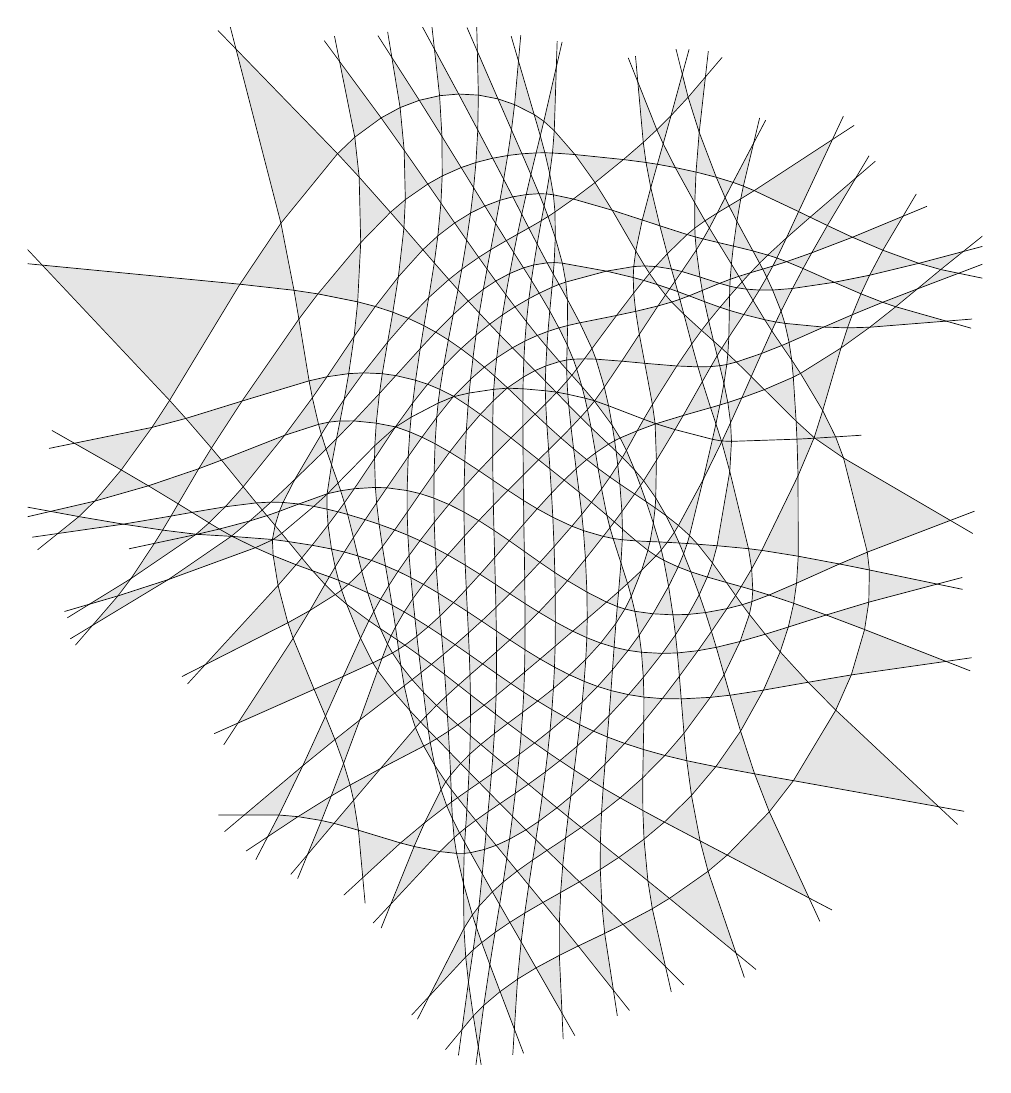
\begin{tikzpicture}[x=\linewidth,y=\linewidth,
  poly/.style={fill=gray!20},
  ext/.style={black,line width=0.25pt},
  lbl/.style={inner sep=0pt,font=\scriptsize},
  plbl/.style={inner sep=0pt,font=\scriptsize}]
\useasboundingbox (0,0) rectangle (1,-1.08636);
\clip (0,0) rectangle (1,-1.08636);
\fill[poly] (0.47774,-1.02397) -- (0.47197,-1.06765) -- (0.46675,-1.03509) -- cycle;
\fill[poly] (0.51306,-0.99657) -- (0.50977,-1.04892) -- (0.49480,-1.00957) -- cycle;
\fill[poly] (0.55688,-0.97162) -- (0.55964,-1.03219) -- (0.53249,-0.98471) -- cycle;
\fill[poly] (0.60434,-0.94861) -- (0.61348,-1.00817) -- (0.57666,-0.96183) -- cycle;
\fill[poly] (0.65424,-0.92282) -- (0.66808,-0.98354) -- (0.62355,-0.93914) -- cycle;
\fill[poly] (0.71263,-0.88360) -- (0.74190,-0.96923) -- (0.67218,-0.91197) -- cycle;
\fill[poly] (0.64962,-0.89365) -- (0.67218,-0.91197) -- (0.65424,-0.92282) -- cycle;
\fill[poly] (0.60131,-0.91731) -- (0.62355,-0.93914) -- (0.60434,-0.94861) -- cycle;
\fill[poly] (0.55690,-0.93734) -- (0.57666,-0.96183) -- (0.55688,-0.97162) -- cycle;
\fill[poly] (0.51685,-0.95755) -- (0.53249,-0.98471) -- (0.51306,-0.99657) -- cycle;
\fill[poly] (0.48409,-0.98124) -- (0.49480,-1.00957) -- (0.47774,-1.02397) -- cycle;
\fill[poly] (0.46167,-0.99963) -- (0.46675,-1.03509) -- (0.45485,-1.04950) -- cycle;
\fill[poly] (0.46663,-0.96583) -- (0.46167,-0.99963) -- (0.45879,-0.97333) -- cycle;
\fill[poly] (0.48951,-0.94764) -- (0.48409,-0.98124) -- (0.47557,-0.95822) -- cycle;
\fill[poly] (0.52062,-0.92734) -- (0.51685,-0.95755) -- (0.50503,-0.93706) -- cycle;
\fill[poly] (0.55823,-0.90578) -- (0.55690,-0.93734) -- (0.53968,-0.91624) -- cycle;
\fill[poly] (0.59976,-0.88164) -- (0.60131,-0.91731) -- (0.57790,-0.89462) -- cycle;
\fill[poly] (0.64555,-0.84994) -- (0.64962,-0.89365) -- (0.61908,-0.86913) -- cycle;
\fill[poly] (0.59982,-0.85374) -- (0.61908,-0.86913) -- (0.59976,-0.88164) -- cycle;
\fill[poly] (0.56038,-0.87769) -- (0.57790,-0.89462) -- (0.55823,-0.90578) -- cycle;
\fill[poly] (0.52482,-0.89811) -- (0.53968,-0.91624) -- (0.52062,-0.92734) -- cycle;
\fill[poly] (0.49432,-0.91840) -- (0.50503,-0.93706) -- (0.48951,-0.94764) -- cycle;
\fill[poly] (0.46994,-0.94220) -- (0.47557,-0.95822) -- (0.46663,-0.96583) -- cycle;
\fill[poly] (0.45699,-0.94331) -- (0.45879,-0.97333) -- (0.42063,-1.01437) -- cycle;
\fill[poly] (0.47268,-0.92024) -- (0.46994,-0.94220) -- (0.46578,-0.92925) -- cycle;
\fill[poly] (0.49808,-0.89487) -- (0.49432,-0.91840) -- (0.48679,-0.90512) -- cycle;
\fill[poly] (0.52887,-0.87183) -- (0.52482,-0.89811) -- (0.51270,-0.88334) -- cycle;
\fill[poly] (0.56336,-0.84882) -- (0.56038,-0.87769) -- (0.54389,-0.86172) -- cycle;
\fill[poly] (0.60105,-0.82215) -- (0.59982,-0.85374) -- (0.57972,-0.83764) -- cycle;
\fill[poly] (0.56605,-0.82663) -- (0.57972,-0.83764) -- (0.56336,-0.84882) -- cycle;
\fill[poly] (0.53227,-0.85037) -- (0.54389,-0.86172) -- (0.52887,-0.87183) -- cycle;
\fill[poly] (0.50183,-0.87006) -- (0.51270,-0.88334) -- (0.49808,-0.89487) -- cycle;
\fill[poly] (0.47613,-0.88615) -- (0.48679,-0.90512) -- (0.47268,-0.92024) -- cycle;
\fill[poly] (0.45645,-0.89645) -- (0.46578,-0.92925) -- (0.45699,-0.94331) -- cycle;
\fill[poly] (0.28313,-0.82635) -- (0.25139,-0.84740) -- (0.26318,-0.82465) -- cycle;
\fill[poly] (0.32086,-0.83338) -- (0.29307,-0.86617) -- (0.30776,-0.83039) -- cycle;
\fill[poly] (0.39049,-0.85391) -- (0.35099,-0.89027) -- (0.34643,-0.84057) -- cycle;
\fill[poly] (0.43171,-0.86296) -- (0.38037,-0.91794) -- (0.40473,-0.85760) -- cycle;
\fill[poly] (0.45718,-0.86483) -- (0.45645,-0.89645) -- (0.44923,-0.86483) -- cycle;
\fill[poly] (0.47851,-0.86066) -- (0.47613,-0.88615) -- (0.46378,-0.86408) -- cycle;
\fill[poly] (0.50467,-0.84997) -- (0.50183,-0.87006) -- (0.49068,-0.85642) -- cycle;
\fill[poly] (0.53516,-0.83144) -- (0.53227,-0.85037) -- (0.52195,-0.84017) -- cycle;
\fill[poly] (0.56883,-0.80514) -- (0.56605,-0.82663) -- (0.55435,-0.81710) -- cycle;
\fill[poly] (0.53901,-0.80445) -- (0.55435,-0.81710) -- (0.53516,-0.83144) -- cycle;
\fill[poly] (0.50781,-0.82597) -- (0.52195,-0.84017) -- (0.50467,-0.84997) -- cycle;
\fill[poly] (0.48011,-0.84350) -- (0.49068,-0.85642) -- (0.47851,-0.86066) -- cycle;
\fill[poly] (0.45774,-0.85331) -- (0.46378,-0.86408) -- (0.45718,-0.86483) -- cycle;
\fill[poly] (0.44667,-0.84843) -- (0.44923,-0.86483) -- (0.43171,-0.86296) -- cycle;
\fill[poly] (0.45873,-0.83816) -- (0.45774,-0.85331) -- (0.45234,-0.84337) -- cycle;
\fill[poly] (0.48221,-0.82118) -- (0.48011,-0.84350) -- (0.46929,-0.83025) -- cycle;
\fill[poly] (0.51071,-0.80191) -- (0.50781,-0.82597) -- (0.49472,-0.81269) -- cycle;
\fill[poly] (0.54227,-0.77946) -- (0.53901,-0.80445) -- (0.52447,-0.79238) -- cycle;
\fill[poly] (0.51283,-0.78270) -- (0.52447,-0.79238) -- (0.51071,-0.80191) -- cycle;
\fill[poly] (0.48400,-0.80179) -- (0.49472,-0.81269) -- (0.48221,-0.82118) -- cycle;
\fill[poly] (0.46001,-0.81876) -- (0.46929,-0.83025) -- (0.45873,-0.83816) -- cycle;
\fill[poly] (0.44491,-0.82870) -- (0.45234,-0.84337) -- (0.44667,-0.84843) -- cycle;
\fill[poly] (0.41568,-0.83285) -- (0.40473,-0.85760) -- (0.39049,-0.85391) -- cycle;
\fill[poly] (0.44401,-0.81104) -- (0.44491,-0.82870) -- (0.43885,-0.81489) -- cycle;
\fill[poly] (0.46127,-0.79879) -- (0.46001,-0.81876) -- (0.45029,-0.80651) -- cycle;
\fill[poly] (0.48574,-0.78183) -- (0.48400,-0.80179) -- (0.47304,-0.79062) -- cycle;
\fill[poly] (0.51500,-0.76109) -- (0.51283,-0.78270) -- (0.49990,-0.77193) -- cycle;
\fill[poly] (0.48734,-0.76146) -- (0.49990,-0.77193) -- (0.48574,-0.78183) -- cycle;
\fill[poly] (0.46230,-0.77964) -- (0.47304,-0.79062) -- (0.46127,-0.79879) -- cycle;
\fill[poly] (0.44352,-0.79769) -- (0.45029,-0.80651) -- (0.44401,-0.81104) -- cycle;
\fill[poly] (0.43302,-0.79812) -- (0.43885,-0.81489) -- (0.41568,-0.83285) -- cycle;
\fill[poly] (0.44299,-0.78280) -- (0.44352,-0.79769) -- (0.43790,-0.78991) -- cycle;
\fill[poly] (0.46306,-0.76094) -- (0.46230,-0.77964) -- (0.45346,-0.77057) -- cycle;
\fill[poly] (0.48883,-0.73928) -- (0.48734,-0.76146) -- (0.47458,-0.75075) -- cycle;
\fill[poly] (0.46355,-0.74140) -- (0.47458,-0.75075) -- (0.46306,-0.76094) -- cycle;
\fill[poly] (0.44182,-0.75858) -- (0.45346,-0.77057) -- (0.44299,-0.78280) -- cycle;
\fill[poly] (0.42632,-0.77248) -- (0.43790,-0.78991) -- (0.43302,-0.79812) -- cycle;
\fill[poly] (0.34139,-0.80919) -- (0.34643,-0.84057) -- (0.32086,-0.83338) -- cycle;
\fill[poly] (0.31794,-0.80467) -- (0.30776,-0.83039) -- (0.28313,-0.82635) -- cycle;
\fill[poly] (0.36960,-0.77602) -- (0.34139,-0.80919) -- (0.33771,-0.79323) -- cycle;
\fill[poly] (0.42162,-0.74871) -- (0.42632,-0.77248) -- (0.41483,-0.75245) -- cycle;
\fill[poly] (0.44064,-0.73694) -- (0.44182,-0.75858) -- (0.42838,-0.74472) -- cycle;
\fill[poly] (0.46379,-0.72053) -- (0.46355,-0.74140) -- (0.45055,-0.73017) -- cycle;
\fill[poly] (0.43968,-0.72049) -- (0.45055,-0.73017) -- (0.44064,-0.73694) -- cycle;
\fill[poly] (0.41955,-0.73563) -- (0.42838,-0.74472) -- (0.42162,-0.74871) -- cycle;
\fill[poly] (0.40616,-0.73317) -- (0.41483,-0.75245) -- (0.36960,-0.77602) -- cycle;
\fill[poly] (0.41756,-0.72065) -- (0.41955,-0.73563) -- (0.41147,-0.72718) -- cycle;
\fill[poly] (0.43840,-0.70015) -- (0.43968,-0.72049) -- (0.42826,-0.70984) -- cycle;
\fill[poly] (0.41450,-0.69601) -- (0.42826,-0.70984) -- (0.41756,-0.72065) -- cycle;
\fill[poly] (0.40023,-0.71505) -- (0.41147,-0.72718) -- (0.40616,-0.73317) -- cycle;
\fill[poly] (0.33090,-0.77061) -- (0.33771,-0.79323) -- (0.31794,-0.80467) -- cycle;
\fill[poly] (0.28818,-0.77303) -- (0.26318,-0.82465) -- (0.22693,-0.82460) -- cycle;
\fill[poly] (0.34782,-0.72510) -- (0.33090,-0.77061) -- (0.32185,-0.74563) -- cycle;
\fill[poly] (0.39436,-0.68928) -- (0.40023,-0.71505) -- (0.38447,-0.69688) -- cycle;
\fill[poly] (0.41203,-0.67547) -- (0.41450,-0.69601) -- (0.40266,-0.68284) -- cycle;
\fill[poly] (0.39079,-0.66784) -- (0.40266,-0.68284) -- (0.39436,-0.68928) -- cycle;
\fill[poly] (0.36653,-0.67328) -- (0.38447,-0.69688) -- (0.34782,-0.72510) -- cycle;
\fill[poly] (0.31190,-0.72106) -- (0.32185,-0.74563) -- (0.28818,-0.77303) -- cycle;
\fill[poly] (0.33054,-0.67942) -- (0.31190,-0.72106) -- (0.30001,-0.69300) -- cycle;
\fill[poly] (0.37112,-0.66061) -- (0.36653,-0.67328) -- (0.36153,-0.66525) -- cycle;
\fill[poly] (0.38844,-0.65114) -- (0.39079,-0.66784) -- (0.38206,-0.65488) -- cycle;
\fill[poly] (0.37686,-0.64561) -- (0.38206,-0.65488) -- (0.37112,-0.66061) -- cycle;
\fill[poly] (0.34864,-0.63951) -- (0.36153,-0.66525) -- (0.33054,-0.67942) -- cycle;
\fill[poly] (0.27805,-0.63956) -- (0.30001,-0.69300) -- (0.22018,-0.72841) -- cycle;
\fill[poly] (0.29557,-0.61045) -- (0.27805,-0.63956) -- (0.27251,-0.62331) -- cycle;
\fill[poly] (0.26223,-0.58416) -- (0.27251,-0.62331) -- (0.18581,-0.66732) -- cycle;
\fill[poly] (0.14736,-0.57802) -- (0.06780,-0.62611) -- (0.09454,-0.59514) -- cycle;
\fill[poly] (0.10821,-0.57701) -- (0.09454,-0.59514) -- (0.06461,-0.60387) -- cycle;
\fill[poly] (0.17599,-0.53091) -- (0.10821,-0.57701) -- (0.13268,-0.54016) -- cycle;
\fill[poly] (0.21358,-0.53245) -- (0.21317,-0.53277) -- (0.17715,-0.53065) -- (0.20078,-0.52511) -- cycle;
\fill[poly] (0.23849,-0.54467) -- (0.14736,-0.57802) -- (0.21317,-0.53277) -- (0.21432,-0.53284) -- cycle;
\fill[poly] (0.28113,-0.56251) -- (0.26223,-0.58416) -- (0.25714,-0.55293) -- cycle;
\fill[poly] (0.25630,-0.53648) -- (0.25714,-0.55293) -- (0.23849,-0.54467) -- cycle;
\fill[poly] (0.27315,-0.53826) -- (0.25693,-0.53611) -- (0.26605,-0.52965) -- cycle;
\fill[poly] (0.29850,-0.56888) -- (0.28113,-0.56251) -- (0.28715,-0.55537) -- cycle;
\fill[poly] (0.32218,-0.59377) -- (0.29557,-0.61045) -- (0.31134,-0.58312) -- cycle;
\fill[poly] (0.35740,-0.62119) -- (0.34864,-0.63951) -- (0.33409,-0.60391) -- cycle;
\fill[poly] (0.38061,-0.63690) -- (0.37686,-0.64561) -- (0.36939,-0.62943) -- cycle;
\fill[poly] (0.39513,-0.64672) -- (0.38844,-0.65114) -- (0.38712,-0.64125) -- cycle;
\fill[poly] (0.42286,-0.66682) -- (0.41203,-0.67547) -- (0.40989,-0.65724) -- cycle;
\fill[poly] (0.45111,-0.68859) -- (0.43840,-0.70015) -- (0.43681,-0.67747) -- cycle;
\fill[poly] (0.47802,-0.70962) -- (0.46379,-0.72053) -- (0.46370,-0.69844) -- cycle;
\fill[poly] (0.50287,-0.72861) -- (0.48883,-0.73928) -- (0.48993,-0.71880) -- cycle;
\fill[poly] (0.53089,-0.74918) -- (0.51500,-0.76109) -- (0.51690,-0.73904) -- cycle;
\fill[poly] (0.55746,-0.76765) -- (0.54227,-0.77946) -- (0.54471,-0.75893) -- cycle;
\fill[poly] (0.58828,-0.78759) -- (0.56883,-0.80514) -- (0.57241,-0.77753) -- cycle;
\fill[poly] (0.62053,-0.80666) -- (0.60105,-0.82215) -- (0.60273,-0.79635) -- cycle;
\fill[poly] (0.66689,-0.83206) -- (0.64555,-0.84994) -- (0.64433,-0.81991) -- cycle;
\fill[poly] (0.73274,-0.86661) -- (0.71263,-0.88360) -- (0.70429,-0.85173) -- cycle;
\fill[poly] (0.77678,-0.82131) -- (0.81840,-0.91153) -- (0.73274,-0.86661) -- cycle;
\fill[poly] (0.69526,-0.80413) -- (0.70429,-0.85173) -- (0.66689,-0.83206) -- cycle;
\fill[poly] (0.64425,-0.78561) -- (0.64433,-0.81991) -- (0.62053,-0.80666) -- cycle;
\fill[poly] (0.60468,-0.77151) -- (0.60273,-0.79635) -- (0.58828,-0.78759) -- cycle;
\fill[poly] (0.57556,-0.75241) -- (0.57241,-0.77753) -- (0.55746,-0.76765) -- cycle;
\fill[poly] (0.54710,-0.73634) -- (0.54471,-0.75893) -- (0.53089,-0.74918) -- cycle;
\fill[poly] (0.51846,-0.71704) -- (0.51690,-0.73904) -- (0.50287,-0.72861) -- cycle;
\fill[poly] (0.49062,-0.69961) -- (0.48993,-0.71880) -- (0.47802,-0.70962) -- cycle;
\fill[poly] (0.46329,-0.67786) -- (0.46370,-0.69844) -- (0.45111,-0.68859) -- cycle;
\fill[poly] (0.43522,-0.65670) -- (0.43681,-0.67747) -- (0.42286,-0.66682) -- cycle;
\fill[poly] (0.40764,-0.63737) -- (0.40989,-0.65724) -- (0.39513,-0.64672) -- cycle;
\fill[poly] (0.38524,-0.62763) -- (0.38712,-0.64125) -- (0.38061,-0.63690) -- cycle;
\fill[poly] (0.36247,-0.61137) -- (0.36939,-0.62943) -- (0.35740,-0.62119) -- cycle;
\fill[poly] (0.32877,-0.58900) -- (0.33409,-0.60391) -- (0.32218,-0.59377) -- cycle;
\fill[poly] (0.31597,-0.57512) -- (0.31134,-0.58312) -- (0.29850,-0.56888) -- cycle;
\fill[poly] (0.33599,-0.58291) -- (0.32877,-0.58900) -- (0.32562,-0.57873) -- cycle;
\fill[poly] (0.36970,-0.59844) -- (0.36247,-0.61137) -- (0.35615,-0.59185) -- cycle;
\fill[poly] (0.39436,-0.61192) -- (0.38524,-0.62763) -- (0.38169,-0.60477) -- cycle;
\fill[poly] (0.41957,-0.62744) -- (0.40764,-0.63737) -- (0.40561,-0.61865) -- cycle;
\fill[poly] (0.44766,-0.64621) -- (0.43522,-0.65670) -- (0.43358,-0.63665) -- cycle;
\fill[poly] (0.47651,-0.66638) -- (0.46329,-0.67786) -- (0.46258,-0.65659) -- cycle;
\fill[poly] (0.50610,-0.68696) -- (0.49062,-0.69961) -- (0.49104,-0.67658) -- cycle;
\fill[poly] (0.53414,-0.70524) -- (0.51846,-0.71704) -- (0.51961,-0.69597) -- cycle;
\fill[poly] (0.56351,-0.72238) -- (0.54710,-0.73634) -- (0.54908,-0.71426) -- cycle;
\fill[poly] (0.59262,-0.73679) -- (0.57556,-0.75241) -- (0.57823,-0.73001) -- cycle;
\fill[poly] (0.62529,-0.74966) -- (0.60468,-0.77151) -- (0.60709,-0.74289) -- cycle;
\fill[poly] (0.66737,-0.76227) -- (0.64425,-0.78561) -- (0.64477,-0.75596) -- cycle;
\fill[poly] (0.72077,-0.77403) -- (0.69526,-0.80413) -- (0.69034,-0.76776) -- cycle;
\fill[poly] (0.80204,-0.78866) -- (0.77678,-0.82131) -- (0.76137,-0.78150) -- cycle;
\fill[poly] (0.74667,-0.73682) -- (0.76137,-0.78150) -- (0.72077,-0.77403) -- cycle;
\fill[poly] (0.68742,-0.73895) -- (0.69034,-0.76776) -- (0.66737,-0.76227) -- cycle;
\fill[poly] (0.64534,-0.72669) -- (0.64477,-0.75596) -- (0.62529,-0.74966) -- cycle;
\fill[poly] (0.60891,-0.72059) -- (0.60709,-0.74289) -- (0.59262,-0.73679) -- cycle;
\fill[poly] (0.58078,-0.70642) -- (0.57823,-0.73001) -- (0.56351,-0.72238) -- cycle;
\fill[poly] (0.55064,-0.69223) -- (0.54908,-0.71426) -- (0.53414,-0.70524) -- cycle;
\fill[poly] (0.52037,-0.67508) -- (0.51961,-0.69597) -- (0.50610,-0.68696) -- cycle;
\fill[poly] (0.49109,-0.65366) -- (0.49104,-0.67658) -- (0.47651,-0.66638) -- cycle;
\fill[poly] (0.46162,-0.63401) -- (0.46258,-0.65659) -- (0.44766,-0.64621) -- cycle;
\fill[poly] (0.43187,-0.61620) -- (0.43358,-0.63665) -- (0.41957,-0.62744) -- cycle;
\fill[poly] (0.40347,-0.59810) -- (0.40561,-0.61865) -- (0.39436,-0.61192) -- cycle;
\fill[poly] (0.37828,-0.58424) -- (0.38169,-0.60477) -- (0.36970,-0.59844) -- cycle;
\fill[poly] (0.34988,-0.56931) -- (0.35615,-0.59185) -- (0.33599,-0.58291) -- cycle;
\fill[poly] (0.32205,-0.56483) -- (0.32562,-0.57873) -- (0.31597,-0.57512) -- cycle;
\fill[poly] (0.29794,-0.54212) -- (0.28715,-0.55537) -- (0.27315,-0.53826) -- cycle;
\fill[poly] (0.33163,-0.54918) -- (0.32205,-0.56483) -- (0.31820,-0.54601) -- cycle;
\fill[poly] (0.36004,-0.55794) -- (0.34988,-0.56931) -- (0.34584,-0.55320) -- cycle;
\fill[poly] (0.38793,-0.56940) -- (0.37828,-0.58424) -- (0.37479,-0.56364) -- cycle;
\fill[poly] (0.41450,-0.58309) -- (0.40347,-0.59810) -- (0.40136,-0.57599) -- cycle;
\fill[poly] (0.44609,-0.60217) -- (0.43187,-0.61620) -- (0.42990,-0.59210) -- cycle;
\fill[poly] (0.47543,-0.62147) -- (0.46162,-0.63401) -- (0.46054,-0.61156) -- cycle;
\fill[poly] (0.50497,-0.64124) -- (0.49109,-0.65366) -- (0.49088,-0.63185) -- cycle;
\fill[poly] (0.53674,-0.66125) -- (0.52037,-0.67508) -- (0.52083,-0.65150) -- cycle;
\fill[poly] (0.56755,-0.67782) -- (0.55064,-0.69223) -- (0.55179,-0.66977) -- cycle;
\fill[poly] (0.59696,-0.69001) -- (0.58078,-0.70642) -- (0.58282,-0.68465) -- cycle;
\fill[poly] (0.62933,-0.69858) -- (0.60891,-0.72059) -- (0.61094,-0.69430) -- cycle;
\fill[poly] (0.66475,-0.70274) -- (0.64534,-0.72669) -- (0.64543,-0.70112) -- cycle;
\fill[poly] (0.71501,-0.70141) -- (0.68742,-0.73895) -- (0.68449,-0.70301) -- cycle;
\fill[poly] (0.77068,-0.69382) -- (0.74667,-0.73682) -- (0.73559,-0.69919) -- cycle;
\fill[poly] (0.72945,-0.67766) -- (0.73559,-0.69919) -- (0.71501,-0.70141) -- cycle;
\fill[poly] (0.68260,-0.67933) -- (0.68449,-0.70301) -- (0.66475,-0.70274) -- cycle;
\fill[poly] (0.64483,-0.68048) -- (0.64543,-0.70112) -- (0.62933,-0.69858) -- cycle;
\fill[poly] (0.61251,-0.67259) -- (0.61094,-0.69430) -- (0.59696,-0.69001) -- cycle;
\fill[poly] (0.58453,-0.66166) -- (0.58282,-0.68465) -- (0.56755,-0.67782) -- cycle;
\fill[poly] (0.55245,-0.64786) -- (0.55179,-0.66977) -- (0.53674,-0.66125) -- cycle;
\fill[poly] (0.52097,-0.62629) -- (0.52083,-0.65150) -- (0.50497,-0.64124) -- cycle;
\fill[poly] (0.49043,-0.60730) -- (0.49088,-0.63185) -- (0.47543,-0.62147) -- cycle;
\fill[poly] (0.45941,-0.58821) -- (0.46054,-0.61156) -- (0.44609,-0.60217) -- cycle;
\fill[poly] (0.42800,-0.56620) -- (0.42990,-0.59210) -- (0.41450,-0.58309) -- cycle;
\fill[poly] (0.39949,-0.55278) -- (0.40136,-0.57599) -- (0.38793,-0.56940) -- cycle;
\fill[poly] (0.37153,-0.54357) -- (0.37479,-0.56364) -- (0.36004,-0.55794) -- cycle;
\fill[poly] (0.34122,-0.53404) -- (0.34584,-0.55320) -- (0.33163,-0.54918) -- cycle;
\fill[poly] (0.31463,-0.52078) -- (0.31820,-0.54601) -- (0.29794,-0.54212) -- cycle;
\fill[poly] (0.32492,-0.50703) -- (0.31463,-0.52078) -- (0.31351,-0.50425) -- cycle;
\fill[poly] (0.35351,-0.51534) -- (0.34122,-0.53404) -- (0.33514,-0.50983) -- cycle;
\fill[poly] (0.38440,-0.52608) -- (0.37153,-0.54357) -- (0.36810,-0.52015) -- cycle;
\fill[poly] (0.41090,-0.53729) -- (0.39949,-0.55278) -- (0.39824,-0.53165) -- cycle;
\fill[poly] (0.43991,-0.55219) -- (0.42800,-0.56620) -- (0.42680,-0.54512) -- cycle;
\fill[poly] (0.47371,-0.57251) -- (0.45941,-0.58821) -- (0.45829,-0.56294) -- cycle;
\fill[poly] (0.50507,-0.59288) -- (0.49043,-0.60730) -- (0.48985,-0.58292) -- cycle;
\fill[poly] (0.53528,-0.61214) -- (0.52097,-0.62629) -- (0.52088,-0.60313) -- cycle;
\fill[poly] (0.57088,-0.63209) -- (0.55245,-0.64786) -- (0.55272,-0.62240) -- cycle;
\fill[poly] (0.60015,-0.64457) -- (0.58453,-0.66166) -- (0.58567,-0.63895) -- cycle;
\fill[poly] (0.62892,-0.65223) -- (0.61251,-0.67259) -- (0.61421,-0.64890) -- cycle;
\fill[poly] (0.66461,-0.65538) -- (0.64483,-0.68048) -- (0.64290,-0.65419) -- cycle;
\fill[poly] (0.70202,-0.65254) -- (0.68260,-0.67933) -- (0.68048,-0.65491) -- cycle;
\fill[poly] (0.74618,-0.64290) -- (0.72945,-0.67766) -- (0.72122,-0.64903) -- cycle;
\fill[poly] (0.71619,-0.63233) -- (0.72122,-0.64903) -- (0.70202,-0.65254) -- cycle;
\fill[poly] (0.67851,-0.63595) -- (0.68048,-0.65491) -- (0.66461,-0.65538) -- cycle;
\fill[poly] (0.64058,-0.63612) -- (0.64290,-0.65419) -- (0.62892,-0.65223) -- cycle;
\fill[poly] (0.61607,-0.62395) -- (0.61421,-0.64890) -- (0.60015,-0.64457) -- cycle;
\fill[poly] (0.58608,-0.61904) -- (0.58567,-0.63895) -- (0.57088,-0.63209) -- cycle;
\fill[poly] (0.55254,-0.59389) -- (0.55272,-0.62240) -- (0.53528,-0.61214) -- cycle;
\fill[poly] (0.52060,-0.57694) -- (0.52088,-0.60313) -- (0.50507,-0.59288) -- cycle;
\fill[poly] (0.48912,-0.55502) -- (0.48985,-0.58292) -- (0.47371,-0.57251) -- cycle;
\fill[poly] (0.45732,-0.53265) -- (0.45829,-0.56294) -- (0.43991,-0.55219) -- cycle;
\fill[poly] (0.42582,-0.51809) -- (0.42680,-0.54512) -- (0.41090,-0.53729) -- cycle;
\fill[poly] (0.39746,-0.50745) -- (0.39824,-0.53165) -- (0.38440,-0.52608) -- cycle;
\fill[poly] (0.36545,-0.49764) -- (0.36810,-0.52015) -- (0.35351,-0.51534) -- cycle;
\fill[poly] (0.33172,-0.49764) -- (0.33514,-0.50983) -- (0.32492,-0.50703) -- cycle;
\fill[poly] (0.31361,-0.48863) -- (0.31351,-0.50425) -- (0.29966,-0.50139) -- cycle;
\fill[poly] (0.34205,-0.48288) -- (0.33172,-0.49764) -- (0.32780,-0.48501) -- cycle;
\fill[poly] (0.37617,-0.48192) -- (0.36545,-0.49764) -- (0.36420,-0.48150) -- cycle;
\fill[poly] (0.41089,-0.48794) -- (0.39746,-0.50745) -- (0.39741,-0.48480) -- cycle;
\fill[poly] (0.44120,-0.49934) -- (0.42582,-0.51809) -- (0.42545,-0.49273) -- cycle;
\fill[poly] (0.47247,-0.51627) -- (0.45732,-0.53265) -- (0.45695,-0.50729) -- cycle;
\fill[poly] (0.50441,-0.53739) -- (0.48912,-0.55502) -- (0.48837,-0.52644) -- cycle;
\fill[poly] (0.53648,-0.55999) -- (0.52060,-0.57694) -- (0.52017,-0.54849) -- cycle;
\fill[poly] (0.56544,-0.57923) -- (0.55254,-0.59389) -- (0.55213,-0.57068) -- cycle;
\fill[poly] (0.60630,-0.60161) -- (0.58608,-0.61904) -- (0.58575,-0.59115) -- cycle;
\fill[poly] (0.62555,-0.60887) -- (0.61607,-0.62395) -- (0.61755,-0.60629) -- cycle;
\fill[poly] (0.65498,-0.61389) -- (0.64058,-0.63612) -- (0.63596,-0.61126) -- cycle;
\fill[poly] (0.69211,-0.61453) -- (0.67851,-0.63595) -- (0.67586,-0.61499) -- cycle;
\fill[poly] (0.73240,-0.60849) -- (0.71619,-0.63233) -- (0.70988,-0.61263) -- cycle;
\fill[poly] (0.70342,-0.59385) -- (0.70988,-0.61263) -- (0.69211,-0.61453) -- cycle;
\fill[poly] (0.67131,-0.58517) -- (0.67586,-0.61499) -- (0.65498,-0.61389) -- cycle;
\fill[poly] (0.63219,-0.59567) -- (0.63596,-0.61126) -- (0.62555,-0.60887) -- cycle;
\fill[poly] (0.61894,-0.59059) -- (0.61755,-0.60629) -- (0.60630,-0.60161) -- cycle;
\fill[poly] (0.64304,-0.56837) -- (0.63219,-0.59567) -- (0.62832,-0.58217) -- cycle;
\fill[poly] (0.62142,-0.56060) -- (0.62832,-0.58217) -- (0.61894,-0.59059) -- cycle;
\fill[poly] (0.58423,-0.55643) -- (0.58575,-0.59115) -- (0.56544,-0.57923) -- cycle;
\fill[poly] (0.55134,-0.54355) -- (0.55213,-0.57068) -- (0.53648,-0.55999) -- cycle;
\fill[poly] (0.51969,-0.51977) -- (0.52017,-0.54849) -- (0.50441,-0.53739) -- cycle;
\fill[poly] (0.48776,-0.50023) -- (0.48837,-0.52644) -- (0.47247,-0.51627) -- cycle;
\fill[poly] (0.45711,-0.48095) -- (0.45695,-0.50729) -- (0.44120,-0.49934) -- cycle;
\fill[poly] (0.42568,-0.46674) -- (0.42545,-0.49273) -- (0.41089,-0.48794) -- cycle;
\fill[poly] (0.39856,-0.44930) -- (0.39741,-0.48480) -- (0.37617,-0.48192) -- cycle;
\fill[poly] (0.36330,-0.45126) -- (0.36420,-0.48150) -- (0.34205,-0.48288) -- cycle;
\fill[poly] (0.32507,-0.47691) -- (0.32780,-0.48501) -- (0.31422,-0.48804) -- cycle;
\fill[poly] (0.38475,-0.41877) -- (0.36330,-0.45126) -- (0.36357,-0.43774) -- cycle;
\fill[poly] (0.41300,-0.42886) -- (0.39856,-0.44930) -- (0.40023,-0.42336) -- cycle;
\fill[poly] (0.44198,-0.44445) -- (0.42568,-0.46674) -- (0.42670,-0.43576) -- cycle;
\fill[poly] (0.47255,-0.46400) -- (0.45711,-0.48095) -- (0.45783,-0.45430) -- cycle;
\fill[poly] (0.50304,-0.48460) -- (0.48776,-0.50023) -- (0.48730,-0.47398) -- cycle;
\fill[poly] (0.53369,-0.50390) -- (0.51969,-0.51977) -- (0.51935,-0.49521) -- cycle;
\fill[poly] (0.56998,-0.52215) -- (0.55134,-0.54355) -- (0.55003,-0.51280) -- cycle;
\fill[poly] (0.60283,-0.53281) -- (0.58423,-0.55643) -- (0.58208,-0.52674) -- cycle;
\fill[poly] (0.62278,-0.53633) -- (0.62142,-0.56060) -- (0.61316,-0.53499) -- cycle;
\fill[poly] (0.60986,-0.52372) -- (0.61316,-0.53499) -- (0.60283,-0.53281) -- cycle;
\fill[poly] (0.58038,-0.50977) -- (0.58208,-0.52674) -- (0.56998,-0.52215) -- cycle;
\fill[poly] (0.54863,-0.48755) -- (0.55003,-0.51280) -- (0.53369,-0.50390) -- cycle;
\fill[poly] (0.51906,-0.46853) -- (0.51935,-0.49521) -- (0.50304,-0.48460) -- cycle;
\fill[poly] (0.48705,-0.44880) -- (0.48730,-0.47398) -- (0.47255,-0.46400) -- cycle;
\fill[poly] (0.45942,-0.42220) -- (0.45783,-0.45430) -- (0.44198,-0.44445) -- cycle;
\fill[poly] (0.42843,-0.40812) -- (0.42670,-0.43576) -- (0.41300,-0.42886) -- cycle;
\fill[poly] (0.40161,-0.40797) -- (0.40023,-0.42336) -- (0.38555,-0.41816) -- cycle;
\fill[poly] (0.44560,-0.38665) -- (0.42843,-0.40812) -- (0.42988,-0.39324) -- cycle;
\fill[poly] (0.47415,-0.40502) -- (0.45942,-0.42220) -- (0.46125,-0.39590) -- cycle;
\fill[poly] (0.50614,-0.42960) -- (0.48705,-0.44880) -- (0.48708,-0.41473) -- cycle;
\fill[poly] (0.53512,-0.45261) -- (0.51906,-0.46853) -- (0.51883,-0.43965) -- cycle;
\fill[poly] (0.56189,-0.47387) -- (0.54863,-0.48755) -- (0.54699,-0.46203) -- cycle;
\fill[poly] (0.59053,-0.49711) -- (0.58038,-0.50977) -- (0.57758,-0.48647) -- cycle;
\fill[poly] (0.61447,-0.51762) -- (0.60986,-0.52372) -- (0.60664,-0.51076) -- cycle;
\fill[poly] (0.63717,-0.53752) -- (0.62278,-0.53633) -- (0.62295,-0.52516) -- cycle;
\fill[poly] (0.65807,-0.55319) -- (0.64304,-0.56837) -- (0.64962,-0.54741) -- cycle;
\fill[poly] (0.68128,-0.56482) -- (0.67131,-0.58517) -- (0.66619,-0.55782) -- cycle;
\fill[poly] (0.71183,-0.57541) -- (0.70342,-0.59385) -- (0.69458,-0.56990) -- cycle;
\fill[poly] (0.68707,-0.55094) -- (0.69458,-0.56990) -- (0.68128,-0.56482) -- cycle;
\fill[poly] (0.66365,-0.54694) -- (0.66619,-0.55782) -- (0.65807,-0.55319) -- cycle;
\fill[poly] (0.65185,-0.53824) -- (0.64962,-0.54741) -- (0.63717,-0.53752) -- cycle;
\fill[poly] (0.66993,-0.53904) -- (0.66365,-0.54694) -- (0.66138,-0.53864) -- cycle;
\fill[poly] (0.69079,-0.54027) -- (0.68707,-0.55094) -- (0.68236,-0.53973) -- cycle;
\fill[poly] (0.67729,-0.52849) -- (0.68236,-0.53973) -- (0.66993,-0.53904) -- cycle;
\fill[poly] (0.65530,-0.51891) -- (0.66138,-0.53864) -- (0.65185,-0.53824) -- cycle;
\fill[poly] (0.62240,-0.50684) -- (0.62295,-0.52516) -- (0.61447,-0.51762) -- cycle;
\fill[poly] (0.60114,-0.48307) -- (0.60664,-0.51076) -- (0.59053,-0.49711) -- cycle;
\fill[poly] (0.57443,-0.46192) -- (0.57758,-0.48647) -- (0.56189,-0.47387) -- cycle;
\fill[poly] (0.54562,-0.44226) -- (0.54699,-0.46203) -- (0.53512,-0.45261) -- cycle;
\fill[poly] (0.51869,-0.41728) -- (0.51883,-0.43965) -- (0.50614,-0.42960) -- cycle;
\fill[poly] (0.48755,-0.39100) -- (0.48708,-0.41473) -- (0.47415,-0.40502) -- cycle;
\fill[poly] (0.46239,-0.38266) -- (0.46125,-0.39590) -- (0.44655,-0.38635) -- cycle;
\fill[poly] (0.50199,-0.37763) -- (0.48755,-0.39100) -- (0.48814,-0.37877) -- cycle;
\fill[poly] (0.53145,-0.40483) -- (0.51869,-0.41728) -- (0.51868,-0.39266) -- cycle;
\fill[poly] (0.55841,-0.42956) -- (0.54562,-0.44226) -- (0.54384,-0.41641) -- cycle;
\fill[poly] (0.58551,-0.45238) -- (0.57443,-0.46192) -- (0.57180,-0.44112) -- cycle;
\fill[poly] (0.60983,-0.47071) -- (0.60114,-0.48307) -- (0.59746,-0.46164) -- cycle;
\fill[poly] (0.63569,-0.48839) -- (0.62240,-0.50684) -- (0.62022,-0.47798) -- cycle;
\fill[poly] (0.65719,-0.50287) -- (0.65530,-0.51891) -- (0.64779,-0.49645) -- cycle;
\fill[poly] (0.68166,-0.52136) -- (0.67729,-0.52849) -- (0.66863,-0.51108) -- cycle;
\fill[poly] (0.70170,-0.54104) -- (0.69079,-0.54027) -- (0.69322,-0.53191) -- cycle;
\fill[poly] (0.73189,-0.58110) -- (0.71183,-0.57541) -- (0.71719,-0.56060) -- cycle;
\fill[poly] (0.74835,-0.60439) -- (0.73240,-0.60849) -- (0.74145,-0.59474) -- cycle;
\fill[poly] (0.77247,-0.63531) -- (0.74618,-0.64290) -- (0.75591,-0.61450) -- cycle;
\fill[poly] (0.81748,-0.68560) -- (0.77068,-0.69382) -- (0.78818,-0.65372) -- cycle;
\fill[poly] (0.95418,-0.81596) -- (0.80204,-0.78866) -- (0.84639,-0.71479) -- cycle;
\fill[poly] (0.86264,-0.67792) -- (0.84639,-0.71479) -- (0.81748,-0.68560) -- cycle;
\fill[poly] (0.79666,-0.62777) -- (0.78818,-0.65372) -- (0.77247,-0.63531) -- cycle;
\fill[poly] (0.75861,-0.60108) -- (0.75591,-0.61450) -- (0.74835,-0.60439) -- cycle;
\fill[poly] (0.74733,-0.58540) -- (0.74145,-0.59474) -- (0.73189,-0.58110) -- cycle;
\fill[poly] (0.77656,-0.59423) -- (0.75861,-0.60108) -- (0.75946,-0.58893) -- cycle;
\fill[poly] (0.83637,-0.61514) -- (0.79666,-0.62777) -- (0.80234,-0.60289) -- cycle;
\fill[poly] (0.96188,-0.66374) -- (0.86264,-0.67792) -- (0.87655,-0.63037) -- cycle;
\fill[poly] (0.88095,-0.60172) -- (0.87655,-0.63037) -- (0.83637,-0.61514) -- cycle;
\fill[poly] (0.80530,-0.58183) -- (0.80234,-0.60289) -- (0.77656,-0.59423) -- cycle;
\fill[poly] (0.75831,-0.56687) -- (0.75946,-0.58893) -- (0.74733,-0.58540) -- cycle;
\fill[poly] (0.72204,-0.54258) -- (0.71719,-0.56060) -- (0.70170,-0.54104) -- cycle;
\fill[poly] (0.76889,-0.54746) -- (0.75831,-0.56687) -- (0.75501,-0.54570) -- cycle;
\fill[poly] (0.85019,-0.56170) -- (0.80530,-0.58183) -- (0.80707,-0.55359) -- cycle;
\fill[poly] (0.95263,-0.58277) -- (0.88095,-0.60172) -- (0.88157,-0.56800) -- cycle;
\fill[poly] (0.87941,-0.54933) -- (0.88157,-0.56800) -- (0.85019,-0.56170) -- cycle;
\fill[poly] (0.80687,-0.46932) -- (0.80707,-0.55359) -- (0.76889,-0.54746) -- cycle;
\fill[poly] (0.73537,-0.46477) -- (0.75501,-0.54570) -- (0.72204,-0.54258) -- cycle;
\fill[poly] (0.70749,-0.47344) -- (0.69322,-0.53191) -- (0.68166,-0.52136) -- cycle;
\fill[poly] (0.65784,-0.49249) -- (0.66863,-0.51108) -- (0.65719,-0.50287) -- cycle;
\fill[poly] (0.64181,-0.47956) -- (0.64779,-0.49645) -- (0.63569,-0.48839) -- cycle;
\fill[poly] (0.65852,-0.45325) -- (0.65784,-0.49249) -- (0.64515,-0.47448) -- cycle;
\fill[poly] (0.63577,-0.46341) -- (0.64515,-0.47448) -- (0.64181,-0.47956) -- cycle;
\fill[poly] (0.61808,-0.45811) -- (0.62022,-0.47798) -- (0.60983,-0.47071) -- cycle;
\fill[poly] (0.62712,-0.44273) -- (0.63577,-0.46341) -- (0.62291,-0.45013) -- cycle;
\fill[poly] (0.61630,-0.44371) -- (0.62291,-0.45013) -- (0.61808,-0.45811) -- cycle;
\fill[poly] (0.59475,-0.44532) -- (0.59746,-0.46164) -- (0.58551,-0.45238) -- cycle;
\fill[poly] (0.61474,-0.43258) -- (0.61630,-0.44371) -- (0.60839,-0.43623) -- cycle;
\fill[poly] (0.63843,-0.42216) -- (0.62712,-0.44273) -- (0.62051,-0.42974) -- cycle;
\fill[poly] (0.61218,-0.41639) -- (0.62051,-0.42974) -- (0.61474,-0.43258) -- cycle;
\fill[poly] (0.59010,-0.41884) -- (0.60839,-0.43623) -- (0.59475,-0.44532) -- cycle;
\fill[poly] (0.56912,-0.41865) -- (0.57180,-0.44112) -- (0.55841,-0.42956) -- cycle;
\fill[poly] (0.58631,-0.39995) -- (0.59010,-0.41884) -- (0.57911,-0.40806) -- cycle;
\fill[poly] (0.56669,-0.39548) -- (0.57911,-0.40806) -- (0.56912,-0.41865) -- cycle;
\fill[poly] (0.54259,-0.39382) -- (0.54384,-0.41641) -- (0.53145,-0.40483) -- cycle;
\fill[poly] (0.51880,-0.37822) -- (0.51868,-0.39266) -- (0.50296,-0.37761) -- cycle;
\fill[poly] (0.55338,-0.38166) -- (0.55393,-0.38223) -- (0.54259,-0.39382) -- (0.54219,-0.38028) -- cycle;
\fill[poly] (0.56571,-0.38396) -- (0.56669,-0.39548) -- (0.55393,-0.38223) -- (0.55433,-0.38181) -- cycle;
\fill[poly] (0.59318,-0.39059) -- (0.59361,-0.39114) -- (0.58631,-0.39995) -- (0.58360,-0.38801) -- cycle;
\fill[poly] (0.60846,-0.39602) -- (0.61218,-0.41639) -- (0.59361,-0.39114) -- (0.59387,-0.39081) -- cycle;
\fill[poly] (0.65715,-0.41454) -- (0.65720,-0.41513) -- (0.63843,-0.42216) -- (0.64520,-0.41013) -- cycle;
\fill[poly] (0.67801,-0.42097) -- (0.65852,-0.45325) -- (0.65720,-0.41513) -- (0.65806,-0.41484) -- cycle;
\fill[poly] (0.72663,-0.43287) -- (0.72690,-0.43377) -- (0.70749,-0.47344) -- (0.71723,-0.43113) -- cycle;
\fill[poly] (0.73715,-0.43329) -- (0.73537,-0.46477) -- (0.72690,-0.43377) -- (0.72730,-0.43294) -- cycle;
\fill[poly] (0.82349,-0.43004) -- (0.80687,-0.46932) -- (0.80575,-0.43099) -- cycle;
\fill[poly] (0.96639,-0.51609) -- (0.87941,-0.54933) -- (0.85453,-0.45073) -- cycle;
\fill[poly] (0.84625,-0.42858) -- (0.85453,-0.45073) -- (0.82451,-0.42998) -- cycle;
\fill[poly] (0.10021,-0.51999) -- (0.03158,-0.52981) -- (0.05363,-0.51209) -- cycle;
\fill[poly] (0.17641,-0.53058) -- (0.17599,-0.53091) -- (0.13268,-0.54016) -- (0.14136,-0.52623) -- cycle;
\fill[poly] (0.15011,-0.51155) -- (0.14136,-0.52623) -- (0.10021,-0.51999) -- cycle;
\fill[poly] (0.07024,-0.49590) -- (0.05363,-0.51209) -- (0.02398,-0.50664) -- cycle;
\fill[poly] (0.12644,-0.47985) -- (0.07024,-0.49590) -- (0.09803,-0.46319) -- cycle;
\fill[poly] (0.17219,-0.50766) -- (0.15011,-0.51155) -- (0.15763,-0.49871) -- cycle;
\fill[poly] (0.20078,-0.52511) -- (0.17715,-0.53065) -- (0.17641,-0.53058) -- (0.18998,-0.51863) -- cycle;
\fill[poly] (0.25633,-0.53605) -- (0.25630,-0.53648) -- (0.23849,-0.54467) -- (0.21432,-0.53284) -- cycle;
\fill[poly] (0.23246,-0.51672) -- (0.21358,-0.53245) -- (0.20078,-0.52511) -- cycle;
\fill[poly] (0.20695,-0.50179) -- (0.18998,-0.51863) -- (0.17219,-0.50766) -- cycle;
\fill[poly] (0.17918,-0.46192) -- (0.15763,-0.49871) -- (0.12644,-0.47985) -- cycle;
\fill[poly] (0.13021,-0.41867) -- (0.09803,-0.46319) -- (0.04893,-0.43525) -- cycle;
\fill[poly] (0.16567,-0.40927) -- (0.13021,-0.41867) -- (0.14864,-0.39036) -- cycle;
\fill[poly] (0.20302,-0.45293) -- (0.17918,-0.46192) -- (0.19246,-0.44031) -- cycle;
\fill[poly] (0.23946,-0.49771) -- (0.20695,-0.50179) -- (0.22574,-0.48083) -- cycle;
\fill[poly] (0.25056,-0.51111) -- (0.23246,-0.51672) -- (0.24563,-0.50519) -- cycle;
\fill[poly] (0.26605,-0.52965) -- (0.25693,-0.53611) -- (0.25633,-0.53605) -- (0.25913,-0.52134) -- cycle;
\fill[poly] (0.26365,-0.50653) -- (0.25913,-0.52134) -- (0.25056,-0.51111) -- cycle;
\fill[poly] (0.25472,-0.49693) -- (0.24563,-0.50519) -- (0.23946,-0.49771) -- cycle;
\fill[poly] (0.28403,-0.49889) -- (0.26365,-0.50653) -- (0.26747,-0.49726) -- cycle;
\fill[poly] (0.31364,-0.48821) -- (0.31361,-0.48863) -- (0.29966,-0.50139) -- (0.28403,-0.49889) -- cycle;
\fill[poly] (0.31825,-0.45778) -- (0.32507,-0.47691) -- (0.31422,-0.48804) -- (0.31364,-0.48821) -- cycle;
\fill[poly] (0.27974,-0.47324) -- (0.26747,-0.49726) -- (0.25472,-0.49693) -- cycle;
\fill[poly] (0.32343,-0.43054) -- (0.31825,-0.45778) -- (0.31254,-0.44143) -- cycle;
\fill[poly] (0.30756,-0.42591) -- (0.31254,-0.44143) -- (0.27974,-0.47324) -- cycle;
\fill[poly] (0.26910,-0.42697) -- (0.22574,-0.48083) -- (0.20302,-0.45293) -- cycle;
\fill[poly] (0.31556,-0.41313) -- (0.30756,-0.42591) -- (0.30467,-0.41548) -- cycle;
\fill[poly] (0.34158,-0.41185) -- (0.32343,-0.43054) -- (0.32716,-0.41188) -- cycle;
\fill[poly] (0.38523,-0.41807) -- (0.38475,-0.41877) -- (0.36357,-0.43774) -- (0.36509,-0.41421) -- cycle;
\fill[poly] (0.40324,-0.39315) -- (0.40161,-0.40797) -- (0.38555,-0.41816) -- (0.38523,-0.41807) -- cycle;
\fill[poly] (0.36842,-0.38319) -- (0.36509,-0.41421) -- (0.34158,-0.41185) -- cycle;
\fill[poly] (0.33158,-0.38910) -- (0.32716,-0.41188) -- (0.31556,-0.41313) -- cycle;
\fill[poly] (0.29818,-0.38763) -- (0.30467,-0.41548) -- (0.26910,-0.42697) -- cycle;
\fill[poly] (0.22450,-0.39109) -- (0.19246,-0.44031) -- (0.16567,-0.40927) -- cycle;
\fill[poly] (0.31350,-0.36562) -- (0.29818,-0.38763) -- (0.29474,-0.36990) -- cycle;
\fill[poly] (0.35155,-0.36154) -- (0.33158,-0.38910) -- (0.33624,-0.36235) -- cycle;
\fill[poly] (0.38560,-0.36437) -- (0.36842,-0.38319) -- (0.37141,-0.36239) -- cycle;
\fill[poly] (0.41891,-0.37345) -- (0.40324,-0.39315) -- (0.40626,-0.36928) -- cycle;
\fill[poly] (0.44610,-0.38609) -- (0.44560,-0.38665) -- (0.42988,-0.39324) -- (0.43176,-0.37885) -- cycle;
\fill[poly] (0.46384,-0.36824) -- (0.46239,-0.38266) -- (0.44655,-0.38635) -- (0.44610,-0.38609) -- cycle;
\fill[poly] (0.43566,-0.35452) -- (0.43176,-0.37885) -- (0.41891,-0.37345) -- cycle;
\fill[poly] (0.41113,-0.33619) -- (0.40626,-0.36928) -- (0.38560,-0.36437) -- cycle;
\fill[poly] (0.37703,-0.32925) -- (0.37141,-0.36239) -- (0.35155,-0.36154) -- cycle;
\fill[poly] (0.34191,-0.32340) -- (0.33624,-0.36235) -- (0.31350,-0.36562) -- cycle;
\fill[poly] (0.28408,-0.30519) -- (0.29474,-0.36990) -- (0.22450,-0.39109) -- cycle;
\fill[poly] (0.22231,-0.26869) -- (0.14864,-0.39036) -- (0.01528,-0.24871) -- cycle;
\fill[poly] (0.30400,-0.27883) -- (0.28408,-0.30519) -- (0.27894,-0.27505) -- cycle;
\fill[poly] (0.36409,-0.29198) -- (0.34191,-0.32340) -- (0.34565,-0.28716) -- cycle;
\fill[poly] (0.39872,-0.30446) -- (0.37703,-0.32925) -- (0.38246,-0.29799) -- cycle;
\fill[poly] (0.42737,-0.31886) -- (0.41113,-0.33619) -- (0.41505,-0.31214) -- cycle;
\fill[poly] (0.45382,-0.33622) -- (0.43566,-0.35452) -- (0.44061,-0.32707) -- cycle;
\fill[poly] (0.47832,-0.35555) -- (0.46384,-0.36824) -- (0.46641,-0.34578) -- cycle;
\fill[poly] (0.50253,-0.37720) -- (0.50199,-0.37763) -- (0.48814,-0.37877) -- (0.48921,-0.36504) -- cycle;
\fill[poly] (0.73621,-0.41372) -- (0.73715,-0.43329) -- (0.72730,-0.43294) -- cycle;
\fill[poly] (0.72086,-0.41497) -- (0.72663,-0.43287) -- (0.71723,-0.43113) -- cycle;
\fill[poly] (0.68662,-0.40618) -- (0.67801,-0.42097) -- (0.65806,-0.41484) -- cycle;
\fill[poly] (0.72503,-0.39517) -- (0.72086,-0.41497) -- (0.71527,-0.39801) -- cycle;
\fill[poly] (0.74797,-0.38778) -- (0.73621,-0.41372) -- (0.73334,-0.39262) -- cycle;
\fill[poly] (0.72926,-0.37264) -- (0.73334,-0.39262) -- (0.72503,-0.39517) -- cycle;
\fill[poly] (0.70661,-0.37076) -- (0.71527,-0.39801) -- (0.68662,-0.40618) -- cycle;
\fill[poly] (0.65435,-0.39467) -- (0.65715,-0.41454) -- (0.64520,-0.41013) -- cycle;
\fill[poly] (0.60397,-0.37655) -- (0.60846,-0.39602) -- (0.59387,-0.39081) -- cycle;
\fill[poly] (0.58045,-0.37574) -- (0.59318,-0.39059) -- (0.58360,-0.38801) -- cycle;
\fill[poly] (0.56487,-0.37008) -- (0.56571,-0.38396) -- (0.55433,-0.38181) -- cycle;
\fill[poly] (0.57508,-0.35754) -- (0.58045,-0.37574) -- (0.56996,-0.36402) -- cycle;
\fill[poly] (0.56458,-0.35807) -- (0.56996,-0.36402) -- (0.56487,-0.37008) -- cycle;
\fill[poly] (0.54221,-0.37019) -- (0.55338,-0.38166) -- (0.54219,-0.38028) -- cycle;
\fill[poly] (0.51904,-0.36601) -- (0.51880,-0.37822) -- (0.50296,-0.37761) -- (0.50253,-0.37720) -- cycle;
\fill[poly] (0.54273,-0.35426) -- (0.54221,-0.37019) -- (0.53137,-0.35919) -- cycle;
\fill[poly] (0.56464,-0.34806) -- (0.56458,-0.35807) -- (0.55704,-0.34968) -- cycle;
\fill[poly] (0.58313,-0.34685) -- (0.57508,-0.35754) -- (0.57143,-0.34725) -- cycle;
\fill[poly] (0.62227,-0.34929) -- (0.60397,-0.37655) -- (0.59524,-0.34722) -- cycle;
\fill[poly] (0.67986,-0.35434) -- (0.65435,-0.39467) -- (0.64634,-0.35154) -- cycle;
\fill[poly] (0.71554,-0.35496) -- (0.70661,-0.37076) -- (0.70203,-0.35524) -- cycle;
\fill[poly] (0.73222,-0.35278) -- (0.72926,-0.37264) -- (0.72480,-0.35408) -- cycle;
\fill[poly] (0.72218,-0.34361) -- (0.72480,-0.35408) -- (0.71554,-0.35496) -- cycle;
\fill[poly] (0.69548,-0.33134) -- (0.70203,-0.35524) -- (0.67986,-0.35434) -- cycle;
\fill[poly] (0.64064,-0.32125) -- (0.64634,-0.35154) -- (0.62227,-0.34929) -- cycle;
\fill[poly] (0.59101,-0.33615) -- (0.59524,-0.34722) -- (0.58313,-0.34685) -- cycle;
\fill[poly] (0.56506,-0.33219) -- (0.57143,-0.34725) -- (0.56464,-0.34806) -- cycle;
\fill[poly] (0.54382,-0.33441) -- (0.55704,-0.34968) -- (0.54273,-0.35426) -- cycle;
\fill[poly] (0.51970,-0.34738) -- (0.53137,-0.35919) -- (0.51904,-0.36601) -- cycle;
\fill[poly] (0.49122,-0.34585) -- (0.48921,-0.36504) -- (0.47832,-0.35555) -- cycle;
\fill[poly] (0.52078,-0.32824) -- (0.51970,-0.34738) -- (0.50777,-0.33527) -- cycle;
\fill[poly] (0.54499,-0.31806) -- (0.54382,-0.33441) -- (0.53379,-0.32232) -- cycle;
\fill[poly] (0.56557,-0.31198) -- (0.56506,-0.33219) -- (0.55638,-0.31444) -- cycle;
\fill[poly] (0.61676,-0.30142) -- (0.59101,-0.33615) -- (0.57832,-0.30910) -- cycle;
\fill[poly] (0.66016,-0.29148) -- (0.64064,-0.32125) -- (0.63682,-0.29714) -- cycle;
\fill[poly] (0.63478,-0.27787) -- (0.63682,-0.29714) -- (0.61676,-0.30142) -- cycle;
\fill[poly] (0.56525,-0.28453) -- (0.57832,-0.30910) -- (0.56557,-0.31198) -- cycle;
\fill[poly] (0.54681,-0.29678) -- (0.55638,-0.31444) -- (0.54499,-0.31806) -- cycle;
\fill[poly] (0.52240,-0.30801) -- (0.53379,-0.32232) -- (0.52078,-0.32824) -- cycle;
\fill[poly] (0.49431,-0.32143) -- (0.50777,-0.33527) -- (0.49122,-0.34585) -- cycle;
\fill[poly] (0.46955,-0.32207) -- (0.46641,-0.34578) -- (0.45382,-0.33622) -- cycle;
\fill[poly] (0.49732,-0.30082) -- (0.49431,-0.32143) -- (0.48390,-0.31051) -- cycle;
\fill[poly] (0.52499,-0.28381) -- (0.52240,-0.30801) -- (0.51034,-0.29237) -- cycle;
\fill[poly] (0.54918,-0.27187) -- (0.54681,-0.29678) -- (0.53586,-0.27810) -- cycle;
\fill[poly] (0.56365,-0.26645) -- (0.56525,-0.28453) -- (0.55656,-0.26887) -- cycle;
\fill[poly] (0.55049,-0.25802) -- (0.55656,-0.26887) -- (0.54918,-0.27187) -- cycle;
\fill[poly] (0.52755,-0.26461) -- (0.53586,-0.27810) -- (0.52499,-0.28381) -- cycle;
\fill[poly] (0.50081,-0.27969) -- (0.51034,-0.29237) -- (0.49732,-0.30082) -- cycle;
\fill[poly] (0.47305,-0.29894) -- (0.48390,-0.31051) -- (0.46955,-0.32207) -- cycle;
\fill[poly] (0.44570,-0.30055) -- (0.44061,-0.32707) -- (0.42737,-0.31886) -- cycle;
\fill[poly] (0.47726,-0.27396) -- (0.47305,-0.29894) -- (0.46145,-0.28638) -- cycle;
\fill[poly] (0.50485,-0.25750) -- (0.50081,-0.27969) -- (0.49023,-0.26536) -- cycle;
\fill[poly] (0.53000,-0.24854) -- (0.52755,-0.26461) -- (0.51932,-0.25156) -- cycle;
\fill[poly] (0.55143,-0.24601) -- (0.55049,-0.25802) -- (0.54403,-0.24630) -- cycle;
\fill[poly] (0.60617,-0.25499) -- (0.56365,-0.26645) -- (0.56001,-0.24665) -- cycle;
\fill[poly] (0.64520,-0.26472) -- (0.63478,-0.27787) -- (0.63424,-0.26169) -- cycle;
\fill[poly] (0.63478,-0.25020) -- (0.63424,-0.26169) -- (0.60617,-0.25499) -- cycle;
\fill[poly] (0.55262,-0.21994) -- (0.56001,-0.24665) -- (0.55143,-0.24601) -- cycle;
\fill[poly] (0.53362,-0.22667) -- (0.54403,-0.24630) -- (0.53000,-0.24854) -- cycle;
\fill[poly] (0.50913,-0.23549) -- (0.51932,-0.25156) -- (0.50485,-0.25750) -- cycle;
\fill[poly] (0.48112,-0.25279) -- (0.49023,-0.26536) -- (0.47726,-0.27396) -- cycle;
\fill[poly] (0.45072,-0.27455) -- (0.46145,-0.28638) -- (0.44570,-0.30055) -- cycle;
\fill[poly] (0.42005,-0.28274) -- (0.41505,-0.31214) -- (0.39872,-0.30446) -- cycle;
\fill[poly] (0.45467,-0.25304) -- (0.45072,-0.27455) -- (0.44113,-0.26378) -- cycle;
\fill[poly] (0.48493,-0.23261) -- (0.48112,-0.25279) -- (0.47240,-0.24058) -- cycle;
\fill[poly] (0.51301,-0.21640) -- (0.50913,-0.23549) -- (0.50128,-0.22301) -- cycle;
\fill[poly] (0.53796,-0.20218) -- (0.53362,-0.22667) -- (0.52485,-0.20976) -- cycle;
\fill[poly] (0.55229,-0.19302) -- (0.55262,-0.21994) -- (0.54506,-0.19780) -- cycle;
\fill[poly] (0.54087,-0.18682) -- (0.54506,-0.19780) -- (0.53796,-0.20218) -- cycle;
\fill[poly] (0.51749,-0.19544) -- (0.52485,-0.20976) -- (0.51301,-0.21640) -- cycle;
\fill[poly] (0.49014,-0.20507) -- (0.50128,-0.22301) -- (0.48493,-0.23261) -- cycle;
\fill[poly] (0.45976,-0.22255) -- (0.47240,-0.24058) -- (0.45467,-0.25304) -- cycle;
\fill[poly] (0.42587,-0.24635) -- (0.44113,-0.26378) -- (0.42005,-0.28274) -- cycle;
\fill[poly] (0.38827,-0.26094) -- (0.38246,-0.29799) -- (0.36409,-0.29198) -- cycle;
\fill[poly] (0.42962,-0.21802) -- (0.42587,-0.24635) -- (0.41393,-0.23256) -- cycle;
\fill[poly] (0.46389,-0.19417) -- (0.45976,-0.22255) -- (0.44725,-0.20453) -- cycle;
\fill[poly] (0.49465,-0.18079) -- (0.49014,-0.20507) -- (0.47885,-0.18677) -- cycle;
\fill[poly] (0.52212,-0.17480) -- (0.51749,-0.19544) -- (0.50808,-0.17716) -- cycle;
\fill[poly] (0.54322,-0.17412) -- (0.54087,-0.18682) -- (0.53557,-0.17389) -- cycle;
\fill[poly] (0.57151,-0.17947) -- (0.55229,-0.19302) -- (0.55063,-0.17504) -- cycle;
\fill[poly] (0.54680,-0.15296) -- (0.55063,-0.17504) -- (0.54322,-0.17412) -- cycle;
\fill[poly] (0.52705,-0.15376) -- (0.53557,-0.17389) -- (0.52212,-0.17480) -- cycle;
\fill[poly] (0.49858,-0.15880) -- (0.50808,-0.17716) -- (0.49465,-0.18079) -- cycle;
\fill[poly] (0.46709,-0.16765) -- (0.47885,-0.18677) -- (0.46389,-0.19417) -- cycle;
\fill[poly] (0.43284,-0.18369) -- (0.44725,-0.20453) -- (0.42962,-0.21802) -- cycle;
\fill[poly] (0.39411,-0.20962) -- (0.41393,-0.23256) -- (0.38827,-0.26094) -- cycle;
\fill[poly] (0.34882,-0.22512) -- (0.34565,-0.28716) -- (0.30400,-0.27883) -- cycle;
\fill[poly] (0.39556,-0.18009) -- (0.39411,-0.20962) -- (0.37993,-0.19334) -- cycle;
\fill[poly] (0.43416,-0.15534) -- (0.43284,-0.18369) -- (0.41906,-0.16380) -- cycle;
\fill[poly] (0.46951,-0.14121) -- (0.46709,-0.16765) -- (0.45406,-0.14652) -- cycle;
\fill[poly] (0.50276,-0.13386) -- (0.49858,-0.15880) -- (0.48702,-0.13672) -- cycle;
\fill[poly] (0.53251,-0.13118) -- (0.52705,-0.15376) -- (0.51770,-0.13210) -- cycle;
\fill[poly] (0.54968,-0.13125) -- (0.54680,-0.15296) -- (0.54171,-0.13103) -- cycle;
\fill[poly] (0.53693,-0.11326) -- (0.54171,-0.13103) -- (0.53251,-0.13118) -- cycle;
\fill[poly] (0.50675,-0.10702) -- (0.51770,-0.13210) -- (0.50276,-0.13386) -- cycle;
\fill[poly] (0.47142,-0.10714) -- (0.48702,-0.13672) -- (0.46951,-0.14121) -- cycle;
\fill[poly] (0.43393,-0.11397) -- (0.45406,-0.14652) -- (0.43416,-0.15534) -- cycle;
\fill[poly] (0.39435,-0.12838) -- (0.41906,-0.16380) -- (0.39556,-0.18009) -- cycle;
\fill[poly] (0.34721,-0.15653) -- (0.37993,-0.19334) -- (0.34882,-0.22512) -- cycle;
\fill[poly] (0.26524,-0.20477) -- (0.27894,-0.27505) -- (0.22231,-0.26869) -- cycle;
\fill[poly] (0.34262,-0.11470) -- (0.34721,-0.15653) -- (0.32454,-0.13199) -- cycle;
\fill[poly] (0.39008,-0.08368) -- (0.39435,-0.12838) -- (0.37021,-0.09448) -- cycle;
\fill[poly] (0.43142,-0.07124) -- (0.43393,-0.11397) -- (0.41021,-0.07607) -- cycle;
\fill[poly] (0.47205,-0.07061) -- (0.47142,-0.10714) -- (0.45140,-0.06952) -- cycle;
\fill[poly] (0.50997,-0.08056) -- (0.50675,-0.10702) -- (0.49259,-0.07459) -- cycle;
\fill[poly] (0.54063,-0.09803) -- (0.53693,-0.11326) -- (0.53048,-0.09098) -- cycle;
\fill[poly] (0.57320,-0.13288) -- (0.54968,-0.13125) -- (0.55155,-0.10795) -- cycle;
\fill[poly] (0.61224,-0.19119) -- (0.57151,-0.17947) -- (0.59421,-0.16228) -- cycle;
\fill[poly] (0.64627,-0.24954) -- (0.63478,-0.25020) -- (0.63691,-0.23378) -- cycle;
\fill[poly] (0.65954,-0.26912) -- (0.64520,-0.26472) -- (0.65129,-0.25738) -- cycle;
\fill[poly] (0.67458,-0.28733) -- (0.66016,-0.29148) -- (0.66799,-0.27989) -- cycle;
\fill[poly] (0.70581,-0.31707) -- (0.69548,-0.33134) -- (0.68730,-0.30012) -- cycle;
\fill[poly] (0.72694,-0.33580) -- (0.72218,-0.34361) -- (0.71830,-0.32811) -- cycle;
\fill[poly] (0.74234,-0.35017) -- (0.73222,-0.35278) -- (0.73335,-0.34168) -- cycle;
\fill[poly] (0.77159,-0.37911) -- (0.74797,-0.38778) -- (0.75789,-0.36544) -- cycle;
\fill[poly] (0.82374,-0.42936) -- (0.82349,-0.43004) -- (0.80575,-0.43099) -- (0.80486,-0.41208) -- cycle;
\fill[poly] (0.83268,-0.40104) -- (0.84625,-0.42858) -- (0.82451,-0.42998) -- (0.82374,-0.42936) -- cycle;
\fill[poly] (0.80192,-0.36603) -- (0.80486,-0.41208) -- (0.77159,-0.37911) -- cycle;
\fill[poly] (0.85183,-0.33551) -- (0.83268,-0.40104) -- (0.80946,-0.36207) -- cycle;
\fill[poly] (0.80022,-0.34807) -- (0.80946,-0.36207) -- (0.80192,-0.36603) -- cycle;
\fill[poly] (0.76862,-0.34126) -- (0.75789,-0.36544) -- (0.74234,-0.35017) -- cycle;
\fill[poly] (0.79752,-0.32963) -- (0.80022,-0.34807) -- (0.78978,-0.33291) -- cycle;
\fill[poly] (0.77936,-0.31745) -- (0.78978,-0.33291) -- (0.76862,-0.34126) -- cycle;
\fill[poly] (0.73437,-0.32415) -- (0.73335,-0.34168) -- (0.72694,-0.33580) -- cycle;
\fill[poly] (0.71337,-0.30726) -- (0.71830,-0.32811) -- (0.70581,-0.31707) -- cycle;
\fill[poly] (0.68312,-0.28448) -- (0.68730,-0.30012) -- (0.67458,-0.28733) -- cycle;
\fill[poly] (0.67246,-0.27342) -- (0.66799,-0.27989) -- (0.65954,-0.26912) -- cycle;
\fill[poly] (0.69277,-0.28084) -- (0.68312,-0.28448) -- (0.68092,-0.27643) -- cycle;
\fill[poly] (0.72514,-0.29285) -- (0.71337,-0.30726) -- (0.70886,-0.28695) -- cycle;
\fill[poly] (0.75005,-0.30044) -- (0.73437,-0.32415) -- (0.73493,-0.29606) -- cycle;
\fill[poly] (0.78361,-0.30824) -- (0.77936,-0.31745) -- (0.77196,-0.30586) -- cycle;
\fill[poly] (0.83367,-0.31361) -- (0.79752,-0.32963) -- (0.79305,-0.30969) -- cycle;
\fill[poly] (0.88202,-0.31374) -- (0.85183,-0.33551) -- (0.85867,-0.31441) -- cycle;
\fill[poly] (0.86371,-0.30064) -- (0.85867,-0.31441) -- (0.83367,-0.31361) -- cycle;
\fill[poly] (0.78906,-0.29691) -- (0.79305,-0.30969) -- (0.78361,-0.30824) -- cycle;
\fill[poly] (0.75971,-0.28555) -- (0.77196,-0.30586) -- (0.75005,-0.30044) -- cycle;
\fill[poly] (0.73513,-0.28115) -- (0.73493,-0.29606) -- (0.72514,-0.29285) -- cycle;
\fill[poly] (0.70653,-0.27523) -- (0.70886,-0.28695) -- (0.69277,-0.28084) -- cycle;
\fill[poly] (0.67790,-0.26564) -- (0.68092,-0.27643) -- (0.67246,-0.27342) -- cycle;
\fill[poly] (0.65759,-0.25014) -- (0.65129,-0.25738) -- (0.64627,-0.24954) -- cycle;
\fill[poly] (0.68509,-0.25536) -- (0.67790,-0.26564) -- (0.67426,-0.25276) -- cycle;
\fill[poly] (0.72467,-0.26778) -- (0.70653,-0.27523) -- (0.70412,-0.26117) -- cycle;
\fill[poly] (0.74279,-0.27237) -- (0.73513,-0.28115) -- (0.73543,-0.27078) -- cycle;
\fill[poly] (0.76633,-0.27484) -- (0.75971,-0.28555) -- (0.75284,-0.27386) -- cycle;
\fill[poly] (0.80109,-0.27316) -- (0.78906,-0.29691) -- (0.78025,-0.27480) -- cycle;
\fill[poly] (0.77411,-0.26144) -- (0.78025,-0.27480) -- (0.76633,-0.27484) -- cycle;
\fill[poly] (0.74830,-0.26618) -- (0.75284,-0.27386) -- (0.74279,-0.27237) -- cycle;
\fill[poly] (0.73581,-0.26353) -- (0.73543,-0.27078) -- (0.72467,-0.26778) -- cycle;
\fill[poly] (0.75697,-0.25669) -- (0.74830,-0.26618) -- (0.74485,-0.26043) -- cycle;
\fill[poly] (0.78044,-0.24971) -- (0.77411,-0.26144) -- (0.76987,-0.25289) -- cycle;
\fill[poly] (0.76658,-0.24661) -- (0.76987,-0.25289) -- (0.75697,-0.25669) -- cycle;
\fill[poly] (0.73706,-0.24757) -- (0.74485,-0.26043) -- (0.73581,-0.26353) -- cycle;
\fill[poly] (0.70032,-0.23282) -- (0.70412,-0.26117) -- (0.68509,-0.25536) -- cycle;
\fill[poly] (0.66989,-0.23686) -- (0.67426,-0.25276) -- (0.65759,-0.25014) -- cycle;
\fill[poly] (0.64371,-0.20141) -- (0.63691,-0.23378) -- (0.61224,-0.19119) -- cycle;
\fill[poly] (0.69067,-0.21666) -- (0.66989,-0.23686) -- (0.66214,-0.20751) -- cycle;
\fill[poly] (0.70749,-0.22127) -- (0.70032,-0.23282) -- (0.69915,-0.21910) -- cycle;
\fill[poly] (0.73915,-0.22878) -- (0.73706,-0.24757) -- (0.72323,-0.22504) -- cycle;
\fill[poly] (0.77518,-0.23818) -- (0.76658,-0.24661) -- (0.75965,-0.23383) -- cycle;
\fill[poly] (0.79493,-0.24506) -- (0.78044,-0.24971) -- (0.78471,-0.24126) -- cycle;
\fill[poly] (0.84475,-0.26669) -- (0.80109,-0.27316) -- (0.81217,-0.25226) -- cycle;
\fill[poly] (0.89545,-0.28763) -- (0.86371,-0.30064) -- (0.87275,-0.27873) -- cycle;
\fill[poly] (0.96208,-0.30734) -- (0.88202,-0.31374) -- (0.90920,-0.29229) -- cycle;
\fill[poly] (0.93179,-0.27363) -- (0.90920,-0.29229) -- (0.89545,-0.28763) -- cycle;
\fill[poly] (0.88185,-0.25927) -- (0.87275,-0.27873) -- (0.84475,-0.26669) -- cycle;
\fill[poly] (0.82123,-0.23580) -- (0.81217,-0.25226) -- (0.79493,-0.24506) -- cycle;
\fill[poly] (0.79471,-0.22025) -- (0.78471,-0.24126) -- (0.77518,-0.23818) -- cycle;
\fill[poly] (0.74283,-0.20281) -- (0.75965,-0.23383) -- (0.73915,-0.22878) -- cycle;
\fill[poly] (0.71398,-0.20985) -- (0.72323,-0.22504) -- (0.70749,-0.22127) -- cycle;
\fill[poly] (0.69876,-0.20991) -- (0.69915,-0.21910) -- (0.69067,-0.21666) -- cycle;
\fill[poly] (0.72229,-0.19404) -- (0.71398,-0.20985) -- (0.70945,-0.20222) -- cycle;
\fill[poly] (0.74684,-0.17933) -- (0.74283,-0.20281) -- (0.73458,-0.18666) -- cycle;
\fill[poly] (0.73049,-0.17799) -- (0.73458,-0.18666) -- (0.72229,-0.19404) -- cycle;
\fill[poly] (0.69870,-0.18350) -- (0.70945,-0.20222) -- (0.69876,-0.20991) -- cycle;
\fill[poly] (0.65263,-0.16755) -- (0.66214,-0.20751) -- (0.64371,-0.20141) -- cycle;
\fill[poly] (0.62398,-0.13813) -- (0.59421,-0.16228) -- (0.57320,-0.13288) -- cycle;
\fill[poly] (0.65953,-0.14305) -- (0.65263,-0.16755) -- (0.64764,-0.14119) -- cycle;
\fill[poly] (0.70002,-0.15122) -- (0.69870,-0.18350) -- (0.67831,-0.14651) -- cycle;
\fill[poly] (0.73872,-0.16201) -- (0.73049,-0.17799) -- (0.72126,-0.15667) -- cycle;
\fill[poly] (0.76095,-0.17065) -- (0.74684,-0.17933) -- (0.74959,-0.16592) -- cycle;
\fill[poly] (0.81955,-0.19849) -- (0.79471,-0.22025) -- (0.80746,-0.19263) -- cycle;
\fill[poly] (0.86383,-0.21950) -- (0.82123,-0.23580) -- (0.83757,-0.20722) -- cycle;
\fill[poly] (0.93339,-0.24681) -- (0.88185,-0.25927) -- (0.89569,-0.23308) -- cycle;
\fill[poly] (0.97506,-0.25721) -- (0.93179,-0.27363) -- (0.95634,-0.25333) -- cycle;
\fill[poly] (0.97989,-0.23444) -- (0.95634,-0.25333) -- (0.93339,-0.24681) -- cycle;
\fill[poly] (0.91683,-0.19750) -- (0.89569,-0.23308) -- (0.86383,-0.21950) -- cycle;
\fill[poly] (0.86727,-0.15751) -- (0.83757,-0.20722) -- (0.81955,-0.19849) -- cycle;
\fill[poly] (0.84287,-0.11717) -- (0.80746,-0.19263) -- (0.76095,-0.17065) -- cycle;
\fill[poly] (0.76034,-0.12091) -- (0.74959,-0.16592) -- (0.73872,-0.16201) -- cycle;
\fill[poly] (0.70336,-0.10965) -- (0.72126,-0.15667) -- (0.70002,-0.15122) -- cycle;
\fill[poly] (0.66563,-0.12157) -- (0.67831,-0.14651) -- (0.65953,-0.14305) -- cycle;
\fill[poly] (0.64476,-0.12015) -- (0.64764,-0.14119) -- (0.62398,-0.13813) -- cycle;
\fill[poly] (0.67381,-0.09218) -- (0.66563,-0.12157) -- (0.65899,-0.10694) -- cycle;
\fill[poly] (0.70986,-0.05161) -- (0.70336,-0.10965) -- (0.69174,-0.07288) -- cycle;
\fill[poly] (0.68566,-0.04873) -- (0.69174,-0.07288) -- (0.67381,-0.09218) -- cycle;
\fill[poly] (0.63905,-0.05681) -- (0.65899,-0.10694) -- (0.64476,-0.12015) -- cycle;
\fill[poly] (0.55370,-0.04128) -- (0.55155,-0.10795) -- (0.54063,-0.09803) -- cycle;
\fill[poly] (0.51405,-0.03496) -- (0.53048,-0.09098) -- (0.50997,-0.08056) -- cycle;
\fill[poly] (0.47096,-0.02476) -- (0.49259,-0.07459) -- (0.47205,-0.07061) -- cycle;
\fill[poly] (0.42603,-0.02246) -- (0.45140,-0.06952) -- (0.43142,-0.07124) -- cycle;
\fill[poly] (0.38143,-0.03116) -- (0.41021,-0.07607) -- (0.39008,-0.08368) -- cycle;
\fill[poly] (0.32668,-0.03538) -- (0.37021,-0.09448) -- (0.34262,-0.11470) -- cycle;
\fill[poly] (0.21818,-0.02238) -- (0.32454,-0.13199) -- (0.26524,-0.20477) -- cycle;
\draw[ext] (0.82976,-0.93615) -- (0.81840,-0.91153) -- (0.77678,-0.82131) -- (0.76137,-0.78150) -- (0.74667,-0.73682) -- (0.73559,-0.69919) -- (0.72945,-0.67766) -- (0.72122,-0.64903) -- (0.71619,-0.63233) -- (0.70988,-0.61263) -- (0.70342,-0.59385) -- (0.69458,-0.56990) -- (0.68707,-0.55094) -- (0.68236,-0.53973) -- (0.67729,-0.52849) -- (0.66863,-0.51108) -- (0.65784,-0.49249) -- (0.64515,-0.47448) -- (0.63577,-0.46341) -- (0.62291,-0.45013) -- (0.61630,-0.44371) -- (0.60839,-0.43623) -- (0.59010,-0.41884) -- (0.57911,-0.40806) -- (0.56669,-0.39548) -- (0.55393,-0.38223) -- (0.55338,-0.38166) -- (0.54221,-0.37019) -- (0.53137,-0.35919) -- (0.51970,-0.34738) -- (0.50777,-0.33527) -- (0.49431,-0.32143) -- (0.48390,-0.31051) -- (0.47305,-0.29894) -- (0.46145,-0.28638) -- (0.45072,-0.27455) -- (0.44113,-0.26378) -- (0.42587,-0.24635) -- (0.41393,-0.23256) -- (0.39411,-0.20962) -- (0.37993,-0.19334) -- (0.34721,-0.15653) -- (0.32454,-0.13199) -- (0.21818,-0.02238) -- (0.19929,-0.00292);
\draw[ext] (0.76285,-0.98644) -- (0.74190,-0.96923) -- (0.67218,-0.91197) -- (0.64962,-0.89365) -- (0.61908,-0.86913) -- (0.59982,-0.85374) -- (0.57972,-0.83764) -- (0.56605,-0.82663) -- (0.55435,-0.81710) -- (0.53901,-0.80445) -- (0.52447,-0.79238) -- (0.51283,-0.78270) -- (0.49990,-0.77193) -- (0.48734,-0.76146) -- (0.47458,-0.75075) -- (0.46355,-0.74140) -- (0.45055,-0.73017) -- (0.43968,-0.72049) -- (0.42826,-0.70984) -- (0.41450,-0.69601) -- (0.40266,-0.68284) -- (0.39079,-0.66784) -- (0.38206,-0.65488) -- (0.37686,-0.64561) -- (0.36939,-0.62943) -- (0.36247,-0.61137) -- (0.35615,-0.59185) -- (0.34988,-0.56931) -- (0.34584,-0.55320) -- (0.34122,-0.53404) -- (0.33514,-0.50983) -- (0.33172,-0.49764) -- (0.32780,-0.48501) -- (0.32507,-0.47691) -- (0.31825,-0.45778) -- (0.31254,-0.44143) -- (0.30756,-0.42591) -- (0.30467,-0.41548) -- (0.29818,-0.38763) -- (0.29474,-0.36990) -- (0.28408,-0.30519) -- (0.27894,-0.27505) -- (0.26524,-0.20477) -- (0.21818,-0.02238) -- (0.21140,0.00387);
\draw[ext] (0.75067,-0.99489) -- (0.74190,-0.96923) -- (0.71263,-0.88360) -- (0.70429,-0.85173) -- (0.69526,-0.80413) -- (0.69034,-0.76776) -- (0.68742,-0.73895) -- (0.68449,-0.70301) -- (0.68260,-0.67933) -- (0.68048,-0.65491) -- (0.67851,-0.63595) -- (0.67586,-0.61499) -- (0.67131,-0.58517) -- (0.66619,-0.55782) -- (0.66365,-0.54694) -- (0.66138,-0.53864) -- (0.65530,-0.51891) -- (0.64779,-0.49645) -- (0.64181,-0.47956) -- (0.63577,-0.46341) -- (0.62712,-0.44273) -- (0.62051,-0.42974) -- (0.61218,-0.41639) -- (0.59361,-0.39114) -- (0.59318,-0.39059) -- (0.58045,-0.37574) -- (0.56996,-0.36402) -- (0.56458,-0.35807) -- (0.55704,-0.34968) -- (0.54382,-0.33441) -- (0.53379,-0.32232) -- (0.52240,-0.30801) -- (0.51034,-0.29237) -- (0.50081,-0.27969) -- (0.49023,-0.26536) -- (0.48112,-0.25279) -- (0.47240,-0.24058) -- (0.45976,-0.22255) -- (0.44725,-0.20453) -- (0.43284,-0.18369) -- (0.41906,-0.16380) -- (0.39435,-0.12838) -- (0.37021,-0.09448) -- (0.32668,-0.03538) -- (0.31060,-0.01355);
\draw[ext] (0.68729,-1.00269) -- (0.66808,-0.98354) -- (0.62355,-0.93914) -- (0.60131,-0.91731) -- (0.57790,-0.89462) -- (0.56038,-0.87769) -- (0.54389,-0.86172) -- (0.53227,-0.85037) -- (0.52195,-0.84017) -- (0.50781,-0.82597) -- (0.49472,-0.81269) -- (0.48400,-0.80179) -- (0.47304,-0.79062) -- (0.46230,-0.77964) -- (0.45346,-0.77057) -- (0.44182,-0.75858) -- (0.42838,-0.74472) -- (0.41955,-0.73563) -- (0.41147,-0.72718) -- (0.40023,-0.71505) -- (0.38447,-0.69688) -- (0.36653,-0.67328) -- (0.36153,-0.66525) -- (0.34864,-0.63951) -- (0.33409,-0.60391) -- (0.32877,-0.58900) -- (0.32562,-0.57873) -- (0.32205,-0.56483) -- (0.31820,-0.54601) -- (0.31463,-0.52078) -- (0.31351,-0.50425) -- (0.31361,-0.48863) -- (0.31364,-0.48821) -- (0.31825,-0.45778) -- (0.32343,-0.43054) -- (0.32716,-0.41188) -- (0.33158,-0.38910) -- (0.33624,-0.36235) -- (0.34191,-0.32340) -- (0.34565,-0.28716) -- (0.34882,-0.22512) -- (0.34721,-0.15653) -- (0.34262,-0.11470) -- (0.32668,-0.03538) -- (0.32134,-0.00880);
\draw[ext] (0.67411,-1.00998) -- (0.66808,-0.98354) -- (0.65424,-0.92282) -- (0.64962,-0.89365) -- (0.64555,-0.84994) -- (0.64433,-0.81991) -- (0.64425,-0.78561) -- (0.64477,-0.75596) -- (0.64534,-0.72669) -- (0.64543,-0.70112) -- (0.64483,-0.68048) -- (0.64290,-0.65419) -- (0.64058,-0.63612) -- (0.63596,-0.61126) -- (0.63219,-0.59567) -- (0.62832,-0.58217) -- (0.62142,-0.56060) -- (0.61316,-0.53499) -- (0.60986,-0.52372) -- (0.60664,-0.51076) -- (0.60114,-0.48307) -- (0.59746,-0.46164) -- (0.59475,-0.44532) -- (0.59010,-0.41884) -- (0.58631,-0.39995) -- (0.58360,-0.38801) -- (0.58045,-0.37574) -- (0.57508,-0.35754) -- (0.57143,-0.34725) -- (0.56506,-0.33219) -- (0.55638,-0.31444) -- (0.54681,-0.29678) -- (0.53586,-0.27810) -- (0.52755,-0.26461) -- (0.51932,-0.25156) -- (0.50913,-0.23549) -- (0.50128,-0.22301) -- (0.49014,-0.20507) -- (0.47885,-0.18677) -- (0.46709,-0.16765) -- (0.45406,-0.14652) -- (0.43393,-0.11397) -- (0.41021,-0.07607) -- (0.38143,-0.03116) -- (0.36680,-0.00833);
\draw[ext] (0.63035,-1.02941) -- (0.61348,-1.00817) -- (0.57666,-0.96183) -- (0.55690,-0.93734) -- (0.53968,-0.91624) -- (0.52482,-0.89811) -- (0.51270,-0.88334) -- (0.50183,-0.87006) -- (0.49068,-0.85642) -- (0.48011,-0.84350) -- (0.46929,-0.83025) -- (0.46001,-0.81876) -- (0.45029,-0.80651) -- (0.44352,-0.79769) -- (0.43790,-0.78991) -- (0.42632,-0.77248) -- (0.41483,-0.75245) -- (0.40616,-0.73317) -- (0.40023,-0.71505) -- (0.39436,-0.68928) -- (0.39079,-0.66784) -- (0.38844,-0.65114) -- (0.38712,-0.64125) -- (0.38524,-0.62763) -- (0.38169,-0.60477) -- (0.37828,-0.58424) -- (0.37479,-0.56364) -- (0.37153,-0.54357) -- (0.36810,-0.52015) -- (0.36545,-0.49764) -- (0.36420,-0.48150) -- (0.36330,-0.45126) -- (0.36357,-0.43774) -- (0.36509,-0.41421) -- (0.36842,-0.38319) -- (0.37141,-0.36239) -- (0.37703,-0.32925) -- (0.38246,-0.29799) -- (0.38827,-0.26094) -- (0.39411,-0.20962) -- (0.39556,-0.18009) -- (0.39435,-0.12838) -- (0.39008,-0.08368) -- (0.38143,-0.03116) -- (0.37702,-0.00441);
\draw[ext] (0.61759,-1.03498) -- (0.61348,-1.00817) -- (0.60434,-0.94861) -- (0.60131,-0.91731) -- (0.59976,-0.88164) -- (0.59982,-0.85374) -- (0.60105,-0.82215) -- (0.60273,-0.79635) -- (0.60468,-0.77151) -- (0.60709,-0.74289) -- (0.60891,-0.72059) -- (0.61094,-0.69430) -- (0.61251,-0.67259) -- (0.61421,-0.64890) -- (0.61607,-0.62395) -- (0.61755,-0.60629) -- (0.61894,-0.59059) -- (0.62142,-0.56060) -- (0.62278,-0.53633) -- (0.62295,-0.52516) -- (0.62240,-0.50684) -- (0.62022,-0.47798) -- (0.61808,-0.45811) -- (0.61630,-0.44371) -- (0.61474,-0.43258) -- (0.61218,-0.41639) -- (0.60846,-0.39602) -- (0.60397,-0.37655) -- (0.59524,-0.34722) -- (0.59101,-0.33615) -- (0.57832,-0.30910) -- (0.56525,-0.28453) -- (0.55656,-0.26887) -- (0.55049,-0.25802) -- (0.54403,-0.24630) -- (0.53362,-0.22667) -- (0.52485,-0.20976) -- (0.51749,-0.19544) -- (0.50808,-0.17716) -- (0.49858,-0.15880) -- (0.48702,-0.13672) -- (0.47142,-0.10714) -- (0.45140,-0.06952) -- (0.42603,-0.02246) -- (0.41316,0.00140);
\draw[ext] (0.57310,-1.05573) -- (0.55964,-1.03219) -- (0.53249,-0.98471) -- (0.51685,-0.95755) -- (0.50503,-0.93706) -- (0.49432,-0.91840) -- (0.48679,-0.90512) -- (0.47613,-0.88615) -- (0.46378,-0.86408) -- (0.45774,-0.85331) -- (0.45234,-0.84337) -- (0.44491,-0.82870) -- (0.43885,-0.81489) -- (0.43302,-0.79812) -- (0.42632,-0.77248) -- (0.42162,-0.74871) -- (0.41955,-0.73563) -- (0.41756,-0.72065) -- (0.41450,-0.69601) -- (0.41203,-0.67547) -- (0.40989,-0.65724) -- (0.40764,-0.63737) -- (0.40561,-0.61865) -- (0.40347,-0.59810) -- (0.40136,-0.57599) -- (0.39949,-0.55278) -- (0.39824,-0.53165) -- (0.39746,-0.50745) -- (0.39741,-0.48480) -- (0.39856,-0.44930) -- (0.40023,-0.42336) -- (0.40161,-0.40797) -- (0.40324,-0.39315) -- (0.40626,-0.36928) -- (0.41113,-0.33619) -- (0.41505,-0.31214) -- (0.42005,-0.28274) -- (0.42587,-0.24635) -- (0.42962,-0.21802) -- (0.43284,-0.18369) -- (0.43416,-0.15534) -- (0.43393,-0.11397) -- (0.43142,-0.07124) -- (0.42603,-0.02246) -- (0.42305,0.00449);
\draw[ext] (0.56087,-1.05928) -- (0.55964,-1.03219) -- (0.55688,-0.97162) -- (0.55690,-0.93734) -- (0.55823,-0.90578) -- (0.56038,-0.87769) -- (0.56336,-0.84882) -- (0.56605,-0.82663) -- (0.56883,-0.80514) -- (0.57241,-0.77753) -- (0.57556,-0.75241) -- (0.57823,-0.73001) -- (0.58078,-0.70642) -- (0.58282,-0.68465) -- (0.58453,-0.66166) -- (0.58567,-0.63895) -- (0.58608,-0.61904) -- (0.58575,-0.59115) -- (0.58423,-0.55643) -- (0.58208,-0.52674) -- (0.58038,-0.50977) -- (0.57758,-0.48647) -- (0.57443,-0.46192) -- (0.57180,-0.44112) -- (0.56912,-0.41865) -- (0.56669,-0.39548) -- (0.56571,-0.38396) -- (0.56487,-0.37008) -- (0.56458,-0.35807) -- (0.56464,-0.34806) -- (0.56506,-0.33219) -- (0.56557,-0.31198) -- (0.56525,-0.28453) -- (0.56365,-0.26645) -- (0.56001,-0.24665) -- (0.55262,-0.21994) -- (0.54506,-0.19780) -- (0.54087,-0.18682) -- (0.53557,-0.17389) -- (0.52705,-0.15376) -- (0.51770,-0.13210) -- (0.50675,-0.10702) -- (0.49259,-0.07459) -- (0.47096,-0.02476) -- (0.46016,0.00011);
\draw[ext] (0.51941,-1.07426) -- (0.50977,-1.04892) -- (0.49480,-1.00957) -- (0.48409,-0.98124) -- (0.47557,-0.95822) -- (0.46994,-0.94220) -- (0.46578,-0.92925) -- (0.45645,-0.89645) -- (0.44923,-0.86483) -- (0.44667,-0.84843) -- (0.44491,-0.82870) -- (0.44401,-0.81104) -- (0.44352,-0.79769) -- (0.44299,-0.78280) -- (0.44182,-0.75858) -- (0.44064,-0.73694) -- (0.43968,-0.72049) -- (0.43840,-0.70015) -- (0.43681,-0.67747) -- (0.43522,-0.65670) -- (0.43358,-0.63665) -- (0.43187,-0.61620) -- (0.42990,-0.59210) -- (0.42800,-0.56620) -- (0.42680,-0.54512) -- (0.42582,-0.51809) -- (0.42545,-0.49273) -- (0.42568,-0.46674) -- (0.42670,-0.43576) -- (0.42843,-0.40812) -- (0.42988,-0.39324) -- (0.43176,-0.37885) -- (0.43566,-0.35452) -- (0.44061,-0.32707) -- (0.44570,-0.30055) -- (0.45072,-0.27455) -- (0.45467,-0.25304) -- (0.45976,-0.22255) -- (0.46389,-0.19417) -- (0.46709,-0.16765) -- (0.46951,-0.14121) -- (0.47142,-0.10714) -- (0.47205,-0.07061) -- (0.47096,-0.02476) -- (0.47031,0.00235);
\draw[ext] (0.50807,-1.07598) -- (0.50977,-1.04892) -- (0.51306,-0.99657) -- (0.51685,-0.95755) -- (0.52062,-0.92734) -- (0.52482,-0.89811) -- (0.52887,-0.87183) -- (0.53227,-0.85037) -- (0.53516,-0.83144) -- (0.53901,-0.80445) -- (0.54227,-0.77946) -- (0.54471,-0.75893) -- (0.54710,-0.73634) -- (0.54908,-0.71426) -- (0.55064,-0.69223) -- (0.55179,-0.66977) -- (0.55245,-0.64786) -- (0.55272,-0.62240) -- (0.55254,-0.59389) -- (0.55213,-0.57068) -- (0.55134,-0.54355) -- (0.55003,-0.51280) -- (0.54863,-0.48755) -- (0.54699,-0.46203) -- (0.54562,-0.44226) -- (0.54384,-0.41641) -- (0.54259,-0.39382) -- (0.54219,-0.38028) -- (0.54221,-0.37019) -- (0.54273,-0.35426) -- (0.54382,-0.33441) -- (0.54499,-0.31806) -- (0.54681,-0.29678) -- (0.54918,-0.27187) -- (0.55049,-0.25802) -- (0.55143,-0.24601) -- (0.55262,-0.21994) -- (0.55229,-0.19302) -- (0.55063,-0.17504) -- (0.54680,-0.15296) -- (0.54171,-0.13103) -- (0.53693,-0.11326) -- (0.53048,-0.09098) -- (0.51405,-0.03496) -- (0.50642,-0.00894);
\draw[ext] (0.47627,-1.09442) -- (0.47197,-1.06765) -- (0.46675,-1.03509) -- (0.46167,-0.99963) -- (0.45879,-0.97333) -- (0.45699,-0.94331) -- (0.45645,-0.89645) -- (0.45718,-0.86483) -- (0.45774,-0.85331) -- (0.45873,-0.83816) -- (0.46001,-0.81876) -- (0.46127,-0.79879) -- (0.46230,-0.77964) -- (0.46306,-0.76094) -- (0.46355,-0.74140) -- (0.46379,-0.72053) -- (0.46370,-0.69844) -- (0.46329,-0.67786) -- (0.46258,-0.65659) -- (0.46162,-0.63401) -- (0.46054,-0.61156) -- (0.45941,-0.58821) -- (0.45829,-0.56294) -- (0.45732,-0.53265) -- (0.45695,-0.50729) -- (0.45711,-0.48095) -- (0.45783,-0.45430) -- (0.45942,-0.42220) -- (0.46125,-0.39590) -- (0.46239,-0.38266) -- (0.46384,-0.36824) -- (0.46641,-0.34578) -- (0.46955,-0.32207) -- (0.47305,-0.29894) -- (0.47726,-0.27396) -- (0.48112,-0.25279) -- (0.48493,-0.23261) -- (0.49014,-0.20507) -- (0.49465,-0.18079) -- (0.49858,-0.15880) -- (0.50276,-0.13386) -- (0.50675,-0.10702) -- (0.50997,-0.08056) -- (0.51405,-0.03496) -- (0.51647,-0.00795);
\draw[ext] (0.46842,-1.09453) -- (0.47197,-1.06765) -- (0.47774,-1.02397) -- (0.48409,-0.98124) -- (0.48951,-0.94764) -- (0.49432,-0.91840) -- (0.49808,-0.89487) -- (0.50183,-0.87006) -- (0.50467,-0.84997) -- (0.50781,-0.82597) -- (0.51071,-0.80191) -- (0.51283,-0.78270) -- (0.51500,-0.76109) -- (0.51690,-0.73904) -- (0.51846,-0.71704) -- (0.51961,-0.69597) -- (0.52037,-0.67508) -- (0.52083,-0.65150) -- (0.52097,-0.62629) -- (0.52088,-0.60313) -- (0.52060,-0.57694) -- (0.52017,-0.54849) -- (0.51969,-0.51977) -- (0.51935,-0.49521) -- (0.51906,-0.46853) -- (0.51883,-0.43965) -- (0.51869,-0.41728) -- (0.51868,-0.39266) -- (0.51880,-0.37822) -- (0.51904,-0.36601) -- (0.51970,-0.34738) -- (0.52078,-0.32824) -- (0.52240,-0.30801) -- (0.52499,-0.28381) -- (0.52755,-0.26461) -- (0.53000,-0.24854) -- (0.53362,-0.22667) -- (0.53796,-0.20218) -- (0.54087,-0.18682) -- (0.54322,-0.17412) -- (0.54680,-0.15296) -- (0.54968,-0.13125) -- (0.55155,-0.10795) -- (0.55370,-0.04128) -- (0.55458,-0.01418);
\draw[ext] (0.45117,-1.07636) -- (0.45485,-1.04950) -- (0.46167,-0.99963) -- (0.46663,-0.96583) -- (0.46994,-0.94220) -- (0.47268,-0.92024) -- (0.47613,-0.88615) -- (0.47851,-0.86066) -- (0.48011,-0.84350) -- (0.48221,-0.82118) -- (0.48400,-0.80179) -- (0.48574,-0.78183) -- (0.48734,-0.76146) -- (0.48883,-0.73928) -- (0.48993,-0.71880) -- (0.49062,-0.69961) -- (0.49104,-0.67658) -- (0.49109,-0.65366) -- (0.49088,-0.63185) -- (0.49043,-0.60730) -- (0.48985,-0.58292) -- (0.48912,-0.55502) -- (0.48837,-0.52644) -- (0.48776,-0.50023) -- (0.48730,-0.47398) -- (0.48705,-0.44880) -- (0.48708,-0.41473) -- (0.48755,-0.39100) -- (0.48814,-0.37877) -- (0.48921,-0.36504) -- (0.49122,-0.34585) -- (0.49431,-0.32143) -- (0.49732,-0.30082) -- (0.50081,-0.27969) -- (0.50485,-0.25750) -- (0.50913,-0.23549) -- (0.51301,-0.21640) -- (0.51749,-0.19544) -- (0.52212,-0.17480) -- (0.52705,-0.15376) -- (0.53251,-0.13118) -- (0.53693,-0.11326) -- (0.54063,-0.09803) -- (0.55370,-0.04128) -- (0.55979,-0.01486);
\draw[ext] (0.43757,-1.07040) -- (0.45485,-1.04950) -- (0.46675,-1.03509) -- (0.47774,-1.02397) -- (0.49480,-1.00957) -- (0.51306,-0.99657) -- (0.53249,-0.98471) -- (0.55688,-0.97162) -- (0.57666,-0.96183) -- (0.60434,-0.94861) -- (0.62355,-0.93914) -- (0.65424,-0.92282) -- (0.67218,-0.91197) -- (0.71263,-0.88360) -- (0.73274,-0.86661) -- (0.77678,-0.82131) -- (0.80204,-0.78866) -- (0.84639,-0.71479) -- (0.86264,-0.67792) -- (0.87655,-0.63037) -- (0.88095,-0.60172) -- (0.88157,-0.56800) -- (0.87941,-0.54933) -- (0.85453,-0.45073) -- (0.84625,-0.42858) -- (0.83268,-0.40104) -- (0.80946,-0.36207) -- (0.80022,-0.34807) -- (0.78978,-0.33291) -- (0.77936,-0.31745) -- (0.77196,-0.30586) -- (0.75971,-0.28555) -- (0.75284,-0.27386) -- (0.74830,-0.26618) -- (0.74485,-0.26043) -- (0.73706,-0.24757) -- (0.72323,-0.22504) -- (0.71398,-0.20985) -- (0.70945,-0.20222) -- (0.69870,-0.18350) -- (0.67831,-0.14651) -- (0.66563,-0.12157) -- (0.65899,-0.10694) -- (0.63905,-0.05681) -- (0.62903,-0.03161);
\draw[ext] (0.40828,-1.03851) -- (0.42063,-1.01437) -- (0.45699,-0.94331) -- (0.46578,-0.92925) -- (0.47268,-0.92024) -- (0.48679,-0.90512) -- (0.49808,-0.89487) -- (0.51270,-0.88334) -- (0.52887,-0.87183) -- (0.54389,-0.86172) -- (0.56336,-0.84882) -- (0.57972,-0.83764) -- (0.60105,-0.82215) -- (0.62053,-0.80666) -- (0.64425,-0.78561) -- (0.66737,-0.76227) -- (0.68742,-0.73895) -- (0.71501,-0.70141) -- (0.72945,-0.67766) -- (0.74618,-0.64290) -- (0.75591,-0.61450) -- (0.75861,-0.60108) -- (0.75946,-0.58893) -- (0.75831,-0.56687) -- (0.75501,-0.54570) -- (0.73537,-0.46477) -- (0.72690,-0.43377) -- (0.72663,-0.43287) -- (0.72086,-0.41497) -- (0.71527,-0.39801) -- (0.70661,-0.37076) -- (0.70203,-0.35524) -- (0.69548,-0.33134) -- (0.68730,-0.30012) -- (0.68312,-0.28448) -- (0.68092,-0.27643) -- (0.67790,-0.26564) -- (0.67426,-0.25276) -- (0.66989,-0.23686) -- (0.66214,-0.20751) -- (0.65263,-0.16755) -- (0.64764,-0.14119) -- (0.64476,-0.12015) -- (0.63905,-0.05681) -- (0.63662,-0.02980);
\draw[ext] (0.40216,-1.03423) -- (0.42063,-1.01437) -- (0.45879,-0.97333) -- (0.46663,-0.96583) -- (0.47557,-0.95822) -- (0.48951,-0.94764) -- (0.50503,-0.93706) -- (0.52062,-0.92734) -- (0.53968,-0.91624) -- (0.55823,-0.90578) -- (0.57790,-0.89462) -- (0.59976,-0.88164) -- (0.61908,-0.86913) -- (0.64555,-0.84994) -- (0.66689,-0.83206) -- (0.69526,-0.80413) -- (0.72077,-0.77403) -- (0.74667,-0.73682) -- (0.77068,-0.69382) -- (0.78818,-0.65372) -- (0.79666,-0.62777) -- (0.80234,-0.60289) -- (0.80530,-0.58183) -- (0.80707,-0.55359) -- (0.80687,-0.46932) -- (0.80575,-0.43099) -- (0.80486,-0.41208) -- (0.80192,-0.36603) -- (0.80022,-0.34807) -- (0.79752,-0.32963) -- (0.79305,-0.30969) -- (0.78906,-0.29691) -- (0.78025,-0.27480) -- (0.77411,-0.26144) -- (0.76987,-0.25289) -- (0.76658,-0.24661) -- (0.75965,-0.23383) -- (0.74283,-0.20281) -- (0.73458,-0.18666) -- (0.73049,-0.17799) -- (0.72126,-0.15667) -- (0.70336,-0.10965) -- (0.69174,-0.07288) -- (0.68566,-0.04873) -- (0.67904,-0.02244);
\draw[ext] (0.37021,-0.94308) -- (0.38037,-0.91794) -- (0.40473,-0.85760) -- (0.41568,-0.83285) -- (0.43302,-0.79812) -- (0.43790,-0.78991) -- (0.44299,-0.78280) -- (0.45346,-0.77057) -- (0.46306,-0.76094) -- (0.47458,-0.75075) -- (0.48883,-0.73928) -- (0.50287,-0.72861) -- (0.51846,-0.71704) -- (0.53414,-0.70524) -- (0.55064,-0.69223) -- (0.56755,-0.67782) -- (0.58453,-0.66166) -- (0.60015,-0.64457) -- (0.61607,-0.62395) -- (0.62555,-0.60887) -- (0.63219,-0.59567) -- (0.64304,-0.56837) -- (0.64962,-0.54741) -- (0.65185,-0.53824) -- (0.65530,-0.51891) -- (0.65719,-0.50287) -- (0.65784,-0.49249) -- (0.65852,-0.45325) -- (0.65720,-0.41513) -- (0.65715,-0.41454) -- (0.65435,-0.39467) -- (0.64634,-0.35154) -- (0.64064,-0.32125) -- (0.63682,-0.29714) -- (0.63478,-0.27787) -- (0.63424,-0.26169) -- (0.63478,-0.25020) -- (0.63691,-0.23378) -- (0.64371,-0.20141) -- (0.65263,-0.16755) -- (0.65953,-0.14305) -- (0.66563,-0.12157) -- (0.67381,-0.09218) -- (0.68566,-0.04873) -- (0.69280,-0.02257);
\draw[ext] (0.36186,-0.93776) -- (0.38037,-0.91794) -- (0.43171,-0.86296) -- (0.44667,-0.84843) -- (0.45234,-0.84337) -- (0.45873,-0.83816) -- (0.46929,-0.83025) -- (0.48221,-0.82118) -- (0.49472,-0.81269) -- (0.51071,-0.80191) -- (0.52447,-0.79238) -- (0.54227,-0.77946) -- (0.55746,-0.76765) -- (0.57556,-0.75241) -- (0.59262,-0.73679) -- (0.60891,-0.72059) -- (0.62933,-0.69858) -- (0.64483,-0.68048) -- (0.66461,-0.65538) -- (0.67851,-0.63595) -- (0.69211,-0.61453) -- (0.70342,-0.59385) -- (0.71183,-0.57541) -- (0.71719,-0.56060) -- (0.72204,-0.54258) -- (0.73537,-0.46477) -- (0.73715,-0.43329) -- (0.73621,-0.41372) -- (0.73334,-0.39262) -- (0.72926,-0.37264) -- (0.72480,-0.35408) -- (0.72218,-0.34361) -- (0.71830,-0.32811) -- (0.71337,-0.30726) -- (0.70886,-0.28695) -- (0.70653,-0.27523) -- (0.70412,-0.26117) -- (0.70032,-0.23282) -- (0.69915,-0.21910) -- (0.69876,-0.20991) -- (0.69870,-0.18350) -- (0.70002,-0.15122) -- (0.70336,-0.10965) -- (0.70986,-0.05161) -- (0.71288,-0.02466);
\draw[ext] (0.35347,-0.91728) -- (0.35099,-0.89027) -- (0.34643,-0.84057) -- (0.34139,-0.80919) -- (0.33771,-0.79323) -- (0.33090,-0.77061) -- (0.32185,-0.74563) -- (0.31190,-0.72106) -- (0.30001,-0.69300) -- (0.27805,-0.63956) -- (0.27251,-0.62331) -- (0.26223,-0.58416) -- (0.25714,-0.55293) -- (0.25630,-0.53648) -- (0.25633,-0.53605) -- (0.25913,-0.52134) -- (0.26365,-0.50653) -- (0.26747,-0.49726) -- (0.27974,-0.47324) -- (0.30756,-0.42591) -- (0.31556,-0.41313) -- (0.33158,-0.38910) -- (0.35155,-0.36154) -- (0.37703,-0.32925) -- (0.39872,-0.30446) -- (0.42005,-0.28274) -- (0.44113,-0.26378) -- (0.45467,-0.25304) -- (0.47240,-0.24058) -- (0.48493,-0.23261) -- (0.50128,-0.22301) -- (0.51301,-0.21640) -- (0.52485,-0.20976) -- (0.53796,-0.20218) -- (0.54506,-0.19780) -- (0.55229,-0.19302) -- (0.57151,-0.17947) -- (0.59421,-0.16228) -- (0.62398,-0.13813) -- (0.64476,-0.12015) -- (0.65899,-0.10694) -- (0.67381,-0.09218) -- (0.69174,-0.07288) -- (0.70986,-0.05161) -- (0.72745,-0.03097);
\draw[ext] (0.33104,-0.90864) -- (0.35099,-0.89027) -- (0.39049,-0.85391) -- (0.41568,-0.83285) -- (0.43885,-0.81489) -- (0.44401,-0.81104) -- (0.45029,-0.80651) -- (0.46127,-0.79879) -- (0.47304,-0.79062) -- (0.48574,-0.78183) -- (0.49990,-0.77193) -- (0.51500,-0.76109) -- (0.53089,-0.74918) -- (0.54710,-0.73634) -- (0.56351,-0.72238) -- (0.58078,-0.70642) -- (0.59696,-0.69001) -- (0.61251,-0.67259) -- (0.62892,-0.65223) -- (0.64058,-0.63612) -- (0.65498,-0.61389) -- (0.67131,-0.58517) -- (0.68128,-0.56482) -- (0.68707,-0.55094) -- (0.69079,-0.54027) -- (0.69322,-0.53191) -- (0.70749,-0.47344) -- (0.71723,-0.43113) -- (0.72086,-0.41497) -- (0.72503,-0.39517) -- (0.72926,-0.37264) -- (0.73222,-0.35278) -- (0.73335,-0.34168) -- (0.73437,-0.32415) -- (0.73493,-0.29606) -- (0.73513,-0.28115) -- (0.73543,-0.27078) -- (0.73581,-0.26353) -- (0.73706,-0.24757) -- (0.73915,-0.22878) -- (0.74283,-0.20281) -- (0.74684,-0.17933) -- (0.74959,-0.16592) -- (0.76034,-0.12091) -- (0.76664,-0.09453);
\draw[ext] (0.28277,-0.89126) -- (0.29307,-0.86617) -- (0.30776,-0.83039) -- (0.31794,-0.80467) -- (0.33090,-0.77061) -- (0.34782,-0.72510) -- (0.36653,-0.67328) -- (0.37112,-0.66061) -- (0.37686,-0.64561) -- (0.38061,-0.63690) -- (0.38524,-0.62763) -- (0.39436,-0.61192) -- (0.40347,-0.59810) -- (0.41450,-0.58309) -- (0.42800,-0.56620) -- (0.43991,-0.55219) -- (0.45732,-0.53265) -- (0.47247,-0.51627) -- (0.48776,-0.50023) -- (0.50304,-0.48460) -- (0.51906,-0.46853) -- (0.53512,-0.45261) -- (0.54562,-0.44226) -- (0.55841,-0.42956) -- (0.56912,-0.41865) -- (0.57911,-0.40806) -- (0.58631,-0.39995) -- (0.59361,-0.39114) -- (0.59387,-0.39081) -- (0.60397,-0.37655) -- (0.62227,-0.34929) -- (0.64064,-0.32125) -- (0.66016,-0.29148) -- (0.66799,-0.27989) -- (0.67246,-0.27342) -- (0.67790,-0.26564) -- (0.68509,-0.25536) -- (0.70032,-0.23282) -- (0.70749,-0.22127) -- (0.71398,-0.20985) -- (0.72229,-0.19404) -- (0.73049,-0.17799) -- (0.73872,-0.16201) -- (0.76034,-0.12091) -- (0.77296,-0.09691);
\draw[ext] (0.27554,-0.88686) -- (0.29307,-0.86617) -- (0.32086,-0.83338) -- (0.34139,-0.80919) -- (0.36960,-0.77602) -- (0.40616,-0.73317) -- (0.41147,-0.72718) -- (0.41756,-0.72065) -- (0.42826,-0.70984) -- (0.43840,-0.70015) -- (0.45111,-0.68859) -- (0.46329,-0.67786) -- (0.47651,-0.66638) -- (0.49109,-0.65366) -- (0.50497,-0.64124) -- (0.52097,-0.62629) -- (0.53528,-0.61214) -- (0.55254,-0.59389) -- (0.56544,-0.57923) -- (0.58423,-0.55643) -- (0.60283,-0.53281) -- (0.60986,-0.52372) -- (0.61447,-0.51762) -- (0.62240,-0.50684) -- (0.63569,-0.48839) -- (0.64181,-0.47956) -- (0.64515,-0.47448) -- (0.65852,-0.45325) -- (0.67801,-0.42097) -- (0.68662,-0.40618) -- (0.70661,-0.37076) -- (0.71554,-0.35496) -- (0.72218,-0.34361) -- (0.72694,-0.33580) -- (0.73437,-0.32415) -- (0.75005,-0.30044) -- (0.75971,-0.28555) -- (0.76633,-0.27484) -- (0.77411,-0.26144) -- (0.78044,-0.24971) -- (0.78471,-0.24126) -- (0.79471,-0.22025) -- (0.80746,-0.19263) -- (0.84287,-0.11717) -- (0.85439,-0.09262);
\draw[ext] (0.23891,-0.87147) -- (0.25139,-0.84740) -- (0.26318,-0.82465) -- (0.28818,-0.77303) -- (0.31190,-0.72106) -- (0.33054,-0.67942) -- (0.34864,-0.63951) -- (0.35740,-0.62119) -- (0.36247,-0.61137) -- (0.36970,-0.59844) -- (0.37828,-0.58424) -- (0.38793,-0.56940) -- (0.39949,-0.55278) -- (0.41090,-0.53729) -- (0.42582,-0.51809) -- (0.44120,-0.49934) -- (0.45711,-0.48095) -- (0.47255,-0.46400) -- (0.48705,-0.44880) -- (0.50614,-0.42960) -- (0.51869,-0.41728) -- (0.53145,-0.40483) -- (0.54259,-0.39382) -- (0.55393,-0.38223) -- (0.55433,-0.38181) -- (0.56487,-0.37008) -- (0.56996,-0.36402) -- (0.57508,-0.35754) -- (0.58313,-0.34685) -- (0.59101,-0.33615) -- (0.61676,-0.30142) -- (0.63478,-0.27787) -- (0.64520,-0.26472) -- (0.65129,-0.25738) -- (0.65759,-0.25014) -- (0.66989,-0.23686) -- (0.69067,-0.21666) -- (0.69876,-0.20991) -- (0.70945,-0.20222) -- (0.72229,-0.19404) -- (0.73458,-0.18666) -- (0.74684,-0.17933) -- (0.76095,-0.17065) -- (0.84287,-0.11717) -- (0.86558,-0.10234);
\draw[ext] (0.22879,-0.86238) -- (0.25139,-0.84740) -- (0.28313,-0.82635) -- (0.31794,-0.80467) -- (0.33771,-0.79323) -- (0.36960,-0.77602) -- (0.41483,-0.75245) -- (0.42162,-0.74871) -- (0.42838,-0.74472) -- (0.44064,-0.73694) -- (0.45055,-0.73017) -- (0.46379,-0.72053) -- (0.47802,-0.70962) -- (0.49062,-0.69961) -- (0.50610,-0.68696) -- (0.52037,-0.67508) -- (0.53674,-0.66125) -- (0.55245,-0.64786) -- (0.57088,-0.63209) -- (0.58608,-0.61904) -- (0.60630,-0.60161) -- (0.61894,-0.59059) -- (0.62832,-0.58217) -- (0.64304,-0.56837) -- (0.65807,-0.55319) -- (0.66365,-0.54694) -- (0.66993,-0.53904) -- (0.67729,-0.52849) -- (0.68166,-0.52136) -- (0.70749,-0.47344) -- (0.72690,-0.43377) -- (0.72730,-0.43294) -- (0.73621,-0.41372) -- (0.74797,-0.38778) -- (0.75789,-0.36544) -- (0.76862,-0.34126) -- (0.77936,-0.31745) -- (0.78361,-0.30824) -- (0.78906,-0.29691) -- (0.80109,-0.27316) -- (0.81217,-0.25226) -- (0.82123,-0.23580) -- (0.83757,-0.20722) -- (0.86727,-0.15751) -- (0.88118,-0.13423);
\draw[ext] (0.20618,-0.84206) -- (0.22693,-0.82460) -- (0.28818,-0.77303) -- (0.32185,-0.74563) -- (0.34782,-0.72510) -- (0.38447,-0.69688) -- (0.39436,-0.68928) -- (0.40266,-0.68284) -- (0.41203,-0.67547) -- (0.42286,-0.66682) -- (0.43522,-0.65670) -- (0.44766,-0.64621) -- (0.46162,-0.63401) -- (0.47543,-0.62147) -- (0.49043,-0.60730) -- (0.50507,-0.59288) -- (0.52060,-0.57694) -- (0.53648,-0.55999) -- (0.55134,-0.54355) -- (0.56998,-0.52215) -- (0.58038,-0.50977) -- (0.59053,-0.49711) -- (0.60114,-0.48307) -- (0.60983,-0.47071) -- (0.61808,-0.45811) -- (0.62291,-0.45013) -- (0.62712,-0.44273) -- (0.63843,-0.42216) -- (0.64520,-0.41013) -- (0.65435,-0.39467) -- (0.67986,-0.35434) -- (0.69548,-0.33134) -- (0.70581,-0.31707) -- (0.71337,-0.30726) -- (0.72514,-0.29285) -- (0.73513,-0.28115) -- (0.74279,-0.27237) -- (0.74830,-0.26618) -- (0.75697,-0.25669) -- (0.76658,-0.24661) -- (0.77518,-0.23818) -- (0.79471,-0.22025) -- (0.81955,-0.19849) -- (0.86727,-0.15751) -- (0.88784,-0.13984);
\draw[ext] (0.19981,-0.82455) -- (0.22693,-0.82460) -- (0.26318,-0.82465) -- (0.28313,-0.82635) -- (0.30776,-0.83039) -- (0.32086,-0.83338) -- (0.34643,-0.84057) -- (0.39049,-0.85391) -- (0.40473,-0.85760) -- (0.43171,-0.86296) -- (0.44923,-0.86483) -- (0.45718,-0.86483) -- (0.46378,-0.86408) -- (0.47851,-0.86066) -- (0.49068,-0.85642) -- (0.50467,-0.84997) -- (0.52195,-0.84017) -- (0.53516,-0.83144) -- (0.55435,-0.81710) -- (0.56883,-0.80514) -- (0.58828,-0.78759) -- (0.60468,-0.77151) -- (0.62529,-0.74966) -- (0.64534,-0.72669) -- (0.66475,-0.70274) -- (0.68260,-0.67933) -- (0.70202,-0.65254) -- (0.71619,-0.63233) -- (0.73240,-0.60849) -- (0.74145,-0.59474) -- (0.74733,-0.58540) -- (0.75831,-0.56687) -- (0.76889,-0.54746) -- (0.80687,-0.46932) -- (0.82349,-0.43004) -- (0.82374,-0.42936) -- (0.83268,-0.40104) -- (0.85183,-0.33551) -- (0.85867,-0.31441) -- (0.86371,-0.30064) -- (0.87275,-0.27873) -- (0.88185,-0.25927) -- (0.89569,-0.23308) -- (0.91683,-0.19750) -- (0.93068,-0.17419);
\draw[ext] (0.20538,-0.75113) -- (0.22018,-0.72841) -- (0.27805,-0.63956) -- (0.29557,-0.61045) -- (0.31134,-0.58312) -- (0.31597,-0.57512) -- (0.32205,-0.56483) -- (0.33163,-0.54918) -- (0.34122,-0.53404) -- (0.35351,-0.51534) -- (0.36545,-0.49764) -- (0.37617,-0.48192) -- (0.39856,-0.44930) -- (0.41300,-0.42886) -- (0.42843,-0.40812) -- (0.44560,-0.38665) -- (0.44610,-0.38609) -- (0.46384,-0.36824) -- (0.47832,-0.35555) -- (0.49122,-0.34585) -- (0.50777,-0.33527) -- (0.52078,-0.32824) -- (0.53379,-0.32232) -- (0.54499,-0.31806) -- (0.55638,-0.31444) -- (0.56557,-0.31198) -- (0.57832,-0.30910) -- (0.61676,-0.30142) -- (0.63682,-0.29714) -- (0.66016,-0.29148) -- (0.67458,-0.28733) -- (0.68312,-0.28448) -- (0.69277,-0.28084) -- (0.70653,-0.27523) -- (0.72467,-0.26778) -- (0.73581,-0.26353) -- (0.74485,-0.26043) -- (0.75697,-0.25669) -- (0.76987,-0.25289) -- (0.78044,-0.24971) -- (0.79493,-0.24506) -- (0.82123,-0.23580) -- (0.86383,-0.21950) -- (0.91683,-0.19750) -- (0.94187,-0.18710);
\draw[ext] (0.19539,-0.73941) -- (0.22018,-0.72841) -- (0.30001,-0.69300) -- (0.33054,-0.67942) -- (0.36153,-0.66525) -- (0.37112,-0.66061) -- (0.38206,-0.65488) -- (0.38844,-0.65114) -- (0.39513,-0.64672) -- (0.40764,-0.63737) -- (0.41957,-0.62744) -- (0.43187,-0.61620) -- (0.44609,-0.60217) -- (0.45941,-0.58821) -- (0.47371,-0.57251) -- (0.48912,-0.55502) -- (0.50441,-0.53739) -- (0.51969,-0.51977) -- (0.53369,-0.50390) -- (0.54863,-0.48755) -- (0.56189,-0.47387) -- (0.57443,-0.46192) -- (0.58551,-0.45238) -- (0.59475,-0.44532) -- (0.60839,-0.43623) -- (0.61474,-0.43258) -- (0.62051,-0.42974) -- (0.63843,-0.42216) -- (0.65720,-0.41513) -- (0.65806,-0.41484) -- (0.68662,-0.40618) -- (0.71527,-0.39801) -- (0.72503,-0.39517) -- (0.73334,-0.39262) -- (0.74797,-0.38778) -- (0.77159,-0.37911) -- (0.80192,-0.36603) -- (0.80946,-0.36207) -- (0.85183,-0.33551) -- (0.88202,-0.31374) -- (0.90920,-0.29229) -- (0.93179,-0.27363) -- (0.95634,-0.25333) -- (0.97989,-0.23444) -- (1.00104,-0.21747);
\draw[ext] (0.16747,-0.68729) -- (0.18581,-0.66732) -- (0.26223,-0.58416) -- (0.28113,-0.56251) -- (0.28715,-0.55537) -- (0.29794,-0.54212) -- (0.31463,-0.52078) -- (0.32492,-0.50703) -- (0.33172,-0.49764) -- (0.34205,-0.48288) -- (0.36330,-0.45126) -- (0.38475,-0.41877) -- (0.38523,-0.41807) -- (0.40324,-0.39315) -- (0.41891,-0.37345) -- (0.43566,-0.35452) -- (0.45382,-0.33622) -- (0.46955,-0.32207) -- (0.48390,-0.31051) -- (0.49732,-0.30082) -- (0.51034,-0.29237) -- (0.52499,-0.28381) -- (0.53586,-0.27810) -- (0.54918,-0.27187) -- (0.55656,-0.26887) -- (0.56365,-0.26645) -- (0.60617,-0.25499) -- (0.63478,-0.25020) -- (0.64627,-0.24954) -- (0.65759,-0.25014) -- (0.67426,-0.25276) -- (0.68509,-0.25536) -- (0.70412,-0.26117) -- (0.72467,-0.26778) -- (0.73543,-0.27078) -- (0.74279,-0.27237) -- (0.75284,-0.27386) -- (0.76633,-0.27484) -- (0.78025,-0.27480) -- (0.80109,-0.27316) -- (0.84475,-0.26669) -- (0.88185,-0.25927) -- (0.93339,-0.24681) -- (0.97989,-0.23444) -- (1.00609,-0.22747);
\draw[ext] (0.16163,-0.67959) -- (0.18581,-0.66732) -- (0.27251,-0.62331) -- (0.29557,-0.61045) -- (0.32218,-0.59377) -- (0.32877,-0.58900) -- (0.33599,-0.58291) -- (0.34988,-0.56931) -- (0.36004,-0.55794) -- (0.37153,-0.54357) -- (0.38440,-0.52608) -- (0.39746,-0.50745) -- (0.41089,-0.48794) -- (0.42568,-0.46674) -- (0.44198,-0.44445) -- (0.45942,-0.42220) -- (0.47415,-0.40502) -- (0.48755,-0.39100) -- (0.50199,-0.37763) -- (0.50253,-0.37720) -- (0.51904,-0.36601) -- (0.53137,-0.35919) -- (0.54273,-0.35426) -- (0.55704,-0.34968) -- (0.56464,-0.34806) -- (0.57143,-0.34725) -- (0.58313,-0.34685) -- (0.59524,-0.34722) -- (0.62227,-0.34929) -- (0.64634,-0.35154) -- (0.67986,-0.35434) -- (0.70203,-0.35524) -- (0.71554,-0.35496) -- (0.72480,-0.35408) -- (0.73222,-0.35278) -- (0.74234,-0.35017) -- (0.76862,-0.34126) -- (0.78978,-0.33291) -- (0.79752,-0.32963) -- (0.83367,-0.31361) -- (0.86371,-0.30064) -- (0.89545,-0.28763) -- (0.93179,-0.27363) -- (0.97506,-0.25721) -- (1.00041,-0.24759);
\draw[ext] (0.05008,-0.64664) -- (0.06780,-0.62611) -- (0.09454,-0.59514) -- (0.10821,-0.57701) -- (0.13268,-0.54016) -- (0.14136,-0.52623) -- (0.15011,-0.51155) -- (0.15763,-0.49871) -- (0.17918,-0.46192) -- (0.19246,-0.44031) -- (0.22450,-0.39109) -- (0.28408,-0.30519) -- (0.30400,-0.27883) -- (0.34882,-0.22512) -- (0.37993,-0.19334) -- (0.39556,-0.18009) -- (0.41906,-0.16380) -- (0.43416,-0.15534) -- (0.45406,-0.14652) -- (0.46951,-0.14121) -- (0.48702,-0.13672) -- (0.50276,-0.13386) -- (0.51770,-0.13210) -- (0.53251,-0.13118) -- (0.54171,-0.13103) -- (0.54968,-0.13125) -- (0.57320,-0.13288) -- (0.62398,-0.13813) -- (0.64764,-0.14119) -- (0.65953,-0.14305) -- (0.67831,-0.14651) -- (0.70002,-0.15122) -- (0.72126,-0.15667) -- (0.73872,-0.16201) -- (0.74959,-0.16592) -- (0.76095,-0.17065) -- (0.80746,-0.19263) -- (0.81955,-0.19849) -- (0.83757,-0.20722) -- (0.86383,-0.21950) -- (0.89569,-0.23308) -- (0.93339,-0.24681) -- (0.95634,-0.25333) -- (0.97506,-0.25721) -- (1.00161,-0.26271);
\draw[ext] (0.04460,-0.64014) -- (0.06780,-0.62611) -- (0.14736,-0.57802) -- (0.21317,-0.53277) -- (0.21358,-0.53245) -- (0.23246,-0.51672) -- (0.24563,-0.50519) -- (0.25472,-0.49693) -- (0.27974,-0.47324) -- (0.31254,-0.44143) -- (0.32343,-0.43054) -- (0.34158,-0.41185) -- (0.36842,-0.38319) -- (0.38560,-0.36437) -- (0.41113,-0.33619) -- (0.42737,-0.31886) -- (0.44570,-0.30055) -- (0.46145,-0.28638) -- (0.47726,-0.27396) -- (0.49023,-0.26536) -- (0.50485,-0.25750) -- (0.51932,-0.25156) -- (0.53000,-0.24854) -- (0.54403,-0.24630) -- (0.55143,-0.24601) -- (0.56001,-0.24665) -- (0.60617,-0.25499) -- (0.63424,-0.26169) -- (0.64520,-0.26472) -- (0.65954,-0.26912) -- (0.67246,-0.27342) -- (0.68092,-0.27643) -- (0.69277,-0.28084) -- (0.70886,-0.28695) -- (0.72514,-0.29285) -- (0.73493,-0.29606) -- (0.75005,-0.30044) -- (0.77196,-0.30586) -- (0.78361,-0.30824) -- (0.79305,-0.30969) -- (0.83367,-0.31361) -- (0.85867,-0.31441) -- (0.88202,-0.31374) -- (0.96208,-0.30734) -- (0.98911,-0.30518);
\draw[ext] (0.04152,-0.61810) -- (0.06461,-0.60387) -- (0.10821,-0.57701) -- (0.17599,-0.53091) -- (0.17641,-0.53058) -- (0.18998,-0.51863) -- (0.20695,-0.50179) -- (0.22574,-0.48083) -- (0.26910,-0.42697) -- (0.29818,-0.38763) -- (0.31350,-0.36562) -- (0.34191,-0.32340) -- (0.36409,-0.29198) -- (0.38827,-0.26094) -- (0.41393,-0.23256) -- (0.42962,-0.21802) -- (0.44725,-0.20453) -- (0.46389,-0.19417) -- (0.47885,-0.18677) -- (0.49465,-0.18079) -- (0.50808,-0.17716) -- (0.52212,-0.17480) -- (0.53557,-0.17389) -- (0.54322,-0.17412) -- (0.55063,-0.17504) -- (0.57151,-0.17947) -- (0.61224,-0.19119) -- (0.64371,-0.20141) -- (0.66214,-0.20751) -- (0.69067,-0.21666) -- (0.69915,-0.21910) -- (0.70749,-0.22127) -- (0.72323,-0.22504) -- (0.73915,-0.22878) -- (0.75965,-0.23383) -- (0.77518,-0.23818) -- (0.78471,-0.24126) -- (0.79493,-0.24506) -- (0.81217,-0.25226) -- (0.84475,-0.26669) -- (0.87275,-0.27873) -- (0.89545,-0.28763) -- (0.90920,-0.29229) -- (0.96208,-0.30734) -- (0.98816,-0.31476);
\draw[ext] (0.03858,-0.61147) -- (0.06461,-0.60387) -- (0.09454,-0.59514) -- (0.14736,-0.57802) -- (0.23849,-0.54467) -- (0.25630,-0.53648) -- (0.25693,-0.53611) -- (0.26605,-0.52965) -- (0.29966,-0.50139) -- (0.31361,-0.48863) -- (0.31422,-0.48804) -- (0.32507,-0.47691) -- (0.36357,-0.43774) -- (0.38475,-0.41877) -- (0.38555,-0.41816) -- (0.40161,-0.40797) -- (0.42988,-0.39324) -- (0.44560,-0.38665) -- (0.44655,-0.38635) -- (0.46239,-0.38266) -- (0.48814,-0.37877) -- (0.50199,-0.37763) -- (0.50296,-0.37761) -- (0.51880,-0.37822) -- (0.54219,-0.38028) -- (0.55338,-0.38166) -- (0.55433,-0.38181) -- (0.56571,-0.38396) -- (0.58360,-0.38801) -- (0.59318,-0.39059) -- (0.59387,-0.39081) -- (0.60846,-0.39602) -- (0.64520,-0.41013) -- (0.65715,-0.41454) -- (0.65806,-0.41484) -- (0.67801,-0.42097) -- (0.71723,-0.43113) -- (0.72663,-0.43287) -- (0.72730,-0.43294) -- (0.73715,-0.43329) -- (0.80575,-0.43099) -- (0.82349,-0.43004) -- (0.82451,-0.42998) -- (0.84625,-0.42858) -- (0.87331,-0.42685);
\draw[ext] (0.10616,-0.54582) -- (0.13268,-0.54016) -- (0.17599,-0.53091) -- (0.17715,-0.53065) -- (0.20078,-0.52511) -- (0.23246,-0.51672) -- (0.25056,-0.51111) -- (0.26365,-0.50653) -- (0.28403,-0.49889) -- (0.31364,-0.48821) -- (0.31422,-0.48804) -- (0.32780,-0.48501) -- (0.34205,-0.48288) -- (0.36420,-0.48150) -- (0.37617,-0.48192) -- (0.39741,-0.48480) -- (0.41089,-0.48794) -- (0.42545,-0.49273) -- (0.44120,-0.49934) -- (0.45695,-0.50729) -- (0.47247,-0.51627) -- (0.48837,-0.52644) -- (0.50441,-0.53739) -- (0.52017,-0.54849) -- (0.53648,-0.55999) -- (0.55213,-0.57068) -- (0.56544,-0.57923) -- (0.58575,-0.59115) -- (0.60630,-0.60161) -- (0.61755,-0.60629) -- (0.62555,-0.60887) -- (0.63596,-0.61126) -- (0.65498,-0.61389) -- (0.67586,-0.61499) -- (0.69211,-0.61453) -- (0.70988,-0.61263) -- (0.73240,-0.60849) -- (0.74835,-0.60439) -- (0.75861,-0.60108) -- (0.77656,-0.59423) -- (0.80530,-0.58183) -- (0.85019,-0.56170) -- (0.87941,-0.54933) -- (0.96639,-0.51609) -- (0.99172,-0.50641);
\draw[ext] (0.01045,-0.54680) -- (0.03158,-0.52981) -- (0.05363,-0.51209) -- (0.07024,-0.49590) -- (0.09803,-0.46319) -- (0.13021,-0.41867) -- (0.14864,-0.39036) -- (0.22231,-0.26869) -- (0.26524,-0.20477) -- (0.32454,-0.13199) -- (0.34262,-0.11470) -- (0.37021,-0.09448) -- (0.39008,-0.08368) -- (0.41021,-0.07607) -- (0.43142,-0.07124) -- (0.45140,-0.06952) -- (0.47205,-0.07061) -- (0.49259,-0.07459) -- (0.50997,-0.08056) -- (0.53048,-0.09098) -- (0.54063,-0.09803) -- (0.55155,-0.10795) -- (0.57320,-0.13288) -- (0.59421,-0.16228) -- (0.61224,-0.19119) -- (0.63691,-0.23378) -- (0.64627,-0.24954) -- (0.65129,-0.25738) -- (0.65954,-0.26912) -- (0.66799,-0.27989) -- (0.67458,-0.28733) -- (0.68730,-0.30012) -- (0.70581,-0.31707) -- (0.71830,-0.32811) -- (0.72694,-0.33580) -- (0.73335,-0.34168) -- (0.74234,-0.35017) -- (0.75789,-0.36544) -- (0.77159,-0.37911) -- (0.80486,-0.41208) -- (0.82374,-0.42936) -- (0.82451,-0.42998) -- (0.85453,-0.45073) -- (0.96639,-0.51609) -- (0.98980,-0.52977);
\draw[ext] (0.00474,-0.53365) -- (0.03158,-0.52981) -- (0.10021,-0.51999) -- (0.15011,-0.51155) -- (0.17219,-0.50766) -- (0.20695,-0.50179) -- (0.23946,-0.49771) -- (0.25472,-0.49693) -- (0.26747,-0.49726) -- (0.28403,-0.49889) -- (0.29966,-0.50139) -- (0.31351,-0.50425) -- (0.32492,-0.50703) -- (0.33514,-0.50983) -- (0.35351,-0.51534) -- (0.36810,-0.52015) -- (0.38440,-0.52608) -- (0.39824,-0.53165) -- (0.41090,-0.53729) -- (0.42680,-0.54512) -- (0.43991,-0.55219) -- (0.45829,-0.56294) -- (0.47371,-0.57251) -- (0.48985,-0.58292) -- (0.50507,-0.59288) -- (0.52088,-0.60313) -- (0.53528,-0.61214) -- (0.55272,-0.62240) -- (0.57088,-0.63209) -- (0.58567,-0.63895) -- (0.60015,-0.64457) -- (0.61421,-0.64890) -- (0.62892,-0.65223) -- (0.64290,-0.65419) -- (0.66461,-0.65538) -- (0.68048,-0.65491) -- (0.70202,-0.65254) -- (0.72122,-0.64903) -- (0.74618,-0.64290) -- (0.77247,-0.63531) -- (0.79666,-0.62777) -- (0.83637,-0.61514) -- (0.88095,-0.60172) -- (0.95263,-0.58277) -- (0.97885,-0.57584);
\draw[ext] (-0.00243,-0.51277) -- (0.02398,-0.50664) -- (0.07024,-0.49590) -- (0.12644,-0.47985) -- (0.17918,-0.46192) -- (0.20302,-0.45293) -- (0.26910,-0.42697) -- (0.30467,-0.41548) -- (0.31556,-0.41313) -- (0.32716,-0.41188) -- (0.34158,-0.41185) -- (0.36509,-0.41421) -- (0.38523,-0.41807) -- (0.38555,-0.41816) -- (0.40023,-0.42336) -- (0.41300,-0.42886) -- (0.42670,-0.43576) -- (0.44198,-0.44445) -- (0.45783,-0.45430) -- (0.47255,-0.46400) -- (0.48730,-0.47398) -- (0.50304,-0.48460) -- (0.51935,-0.49521) -- (0.53369,-0.50390) -- (0.55003,-0.51280) -- (0.56998,-0.52215) -- (0.58208,-0.52674) -- (0.60283,-0.53281) -- (0.61316,-0.53499) -- (0.62278,-0.53633) -- (0.63717,-0.53752) -- (0.65185,-0.53824) -- (0.66138,-0.53864) -- (0.66993,-0.53904) -- (0.68236,-0.53973) -- (0.69079,-0.54027) -- (0.70170,-0.54104) -- (0.72204,-0.54258) -- (0.75501,-0.54570) -- (0.76889,-0.54746) -- (0.80707,-0.55359) -- (0.85019,-0.56170) -- (0.88157,-0.56800) -- (0.95263,-0.58277) -- (0.97918,-0.58829);
\draw[ext] (-0.00269,-0.50174) -- (0.02398,-0.50664) -- (0.05363,-0.51209) -- (0.10021,-0.51999) -- (0.14136,-0.52623) -- (0.17641,-0.53058) -- (0.17715,-0.53065) -- (0.21317,-0.53277) -- (0.21432,-0.53284) -- (0.25633,-0.53605) -- (0.25693,-0.53611) -- (0.27315,-0.53826) -- (0.29794,-0.54212) -- (0.31820,-0.54601) -- (0.33163,-0.54918) -- (0.34584,-0.55320) -- (0.36004,-0.55794) -- (0.37479,-0.56364) -- (0.38793,-0.56940) -- (0.40136,-0.57599) -- (0.41450,-0.58309) -- (0.42990,-0.59210) -- (0.44609,-0.60217) -- (0.46054,-0.61156) -- (0.47543,-0.62147) -- (0.49088,-0.63185) -- (0.50497,-0.64124) -- (0.52083,-0.65150) -- (0.53674,-0.66125) -- (0.55179,-0.66977) -- (0.56755,-0.67782) -- (0.58282,-0.68465) -- (0.59696,-0.69001) -- (0.61094,-0.69430) -- (0.62933,-0.69858) -- (0.64543,-0.70112) -- (0.66475,-0.70274) -- (0.68449,-0.70301) -- (0.71501,-0.70141) -- (0.73559,-0.69919) -- (0.77068,-0.69382) -- (0.81748,-0.68560) -- (0.86264,-0.67792) -- (0.96188,-0.66374) -- (0.98872,-0.65990);
\draw[ext] (0.02236,-0.44067) -- (0.04893,-0.43525) -- (0.13021,-0.41867) -- (0.16567,-0.40927) -- (0.22450,-0.39109) -- (0.29474,-0.36990) -- (0.31350,-0.36562) -- (0.33624,-0.36235) -- (0.35155,-0.36154) -- (0.37141,-0.36239) -- (0.38560,-0.36437) -- (0.40626,-0.36928) -- (0.41891,-0.37345) -- (0.43176,-0.37885) -- (0.44610,-0.38609) -- (0.44655,-0.38635) -- (0.46125,-0.39590) -- (0.47415,-0.40502) -- (0.48708,-0.41473) -- (0.50614,-0.42960) -- (0.51883,-0.43965) -- (0.53512,-0.45261) -- (0.54699,-0.46203) -- (0.56189,-0.47387) -- (0.57758,-0.48647) -- (0.59053,-0.49711) -- (0.60664,-0.51076) -- (0.61447,-0.51762) -- (0.62295,-0.52516) -- (0.63717,-0.53752) -- (0.64962,-0.54741) -- (0.65807,-0.55319) -- (0.66619,-0.55782) -- (0.68128,-0.56482) -- (0.69458,-0.56990) -- (0.71183,-0.57541) -- (0.73189,-0.58110) -- (0.74733,-0.58540) -- (0.75946,-0.58893) -- (0.77656,-0.59423) -- (0.80234,-0.60289) -- (0.83637,-0.61514) -- (0.87655,-0.63037) -- (0.96188,-0.66374) -- (0.98713,-0.67362);
\draw[ext] (0.02537,-0.42183) -- (0.04893,-0.43525) -- (0.09803,-0.46319) -- (0.12644,-0.47985) -- (0.15763,-0.49871) -- (0.17219,-0.50766) -- (0.18998,-0.51863) -- (0.20078,-0.52511) -- (0.21358,-0.53245) -- (0.21432,-0.53284) -- (0.23849,-0.54467) -- (0.25714,-0.55293) -- (0.28113,-0.56251) -- (0.29850,-0.56888) -- (0.31597,-0.57512) -- (0.32562,-0.57873) -- (0.33599,-0.58291) -- (0.35615,-0.59185) -- (0.36970,-0.59844) -- (0.38169,-0.60477) -- (0.39436,-0.61192) -- (0.40561,-0.61865) -- (0.41957,-0.62744) -- (0.43358,-0.63665) -- (0.44766,-0.64621) -- (0.46258,-0.65659) -- (0.47651,-0.66638) -- (0.49104,-0.67658) -- (0.50610,-0.68696) -- (0.51961,-0.69597) -- (0.53414,-0.70524) -- (0.54908,-0.71426) -- (0.56351,-0.72238) -- (0.57823,-0.73001) -- (0.59262,-0.73679) -- (0.60709,-0.74289) -- (0.62529,-0.74966) -- (0.64477,-0.75596) -- (0.66737,-0.76227) -- (0.69034,-0.76776) -- (0.72077,-0.77403) -- (0.76137,-0.78150) -- (0.80204,-0.78866) -- (0.95418,-0.81596) -- (0.98087,-0.82075);
\draw[ext] (-0.01172,-0.24611) -- (0.01528,-0.24871) -- (0.22231,-0.26869) -- (0.27894,-0.27505) -- (0.30400,-0.27883) -- (0.34565,-0.28716) -- (0.36409,-0.29198) -- (0.38246,-0.29799) -- (0.39872,-0.30446) -- (0.41505,-0.31214) -- (0.42737,-0.31886) -- (0.44061,-0.32707) -- (0.45382,-0.33622) -- (0.46641,-0.34578) -- (0.47832,-0.35555) -- (0.48921,-0.36504) -- (0.50253,-0.37720) -- (0.50296,-0.37761) -- (0.51868,-0.39266) -- (0.53145,-0.40483) -- (0.54384,-0.41641) -- (0.55841,-0.42956) -- (0.57180,-0.44112) -- (0.58551,-0.45238) -- (0.59746,-0.46164) -- (0.60983,-0.47071) -- (0.62022,-0.47798) -- (0.63569,-0.48839) -- (0.64779,-0.49645) -- (0.65719,-0.50287) -- (0.66863,-0.51108) -- (0.68166,-0.52136) -- (0.69322,-0.53191) -- (0.70170,-0.54104) -- (0.71719,-0.56060) -- (0.73189,-0.58110) -- (0.74145,-0.59474) -- (0.74835,-0.60439) -- (0.75591,-0.61450) -- (0.77247,-0.63531) -- (0.78818,-0.65372) -- (0.81748,-0.68560) -- (0.84639,-0.71479) -- (0.95418,-0.81596) -- (0.97395,-0.83452);
\draw[ext] (-0.00331,-0.22897) -- (0.01528,-0.24871) -- (0.14864,-0.39036) -- (0.16567,-0.40927) -- (0.19246,-0.44031) -- (0.20302,-0.45293) -- (0.22574,-0.48083) -- (0.23946,-0.49771) -- (0.24563,-0.50519) -- (0.25056,-0.51111) -- (0.25913,-0.52134) -- (0.26605,-0.52965) -- (0.27315,-0.53826) -- (0.28715,-0.55537) -- (0.29850,-0.56888) -- (0.31134,-0.58312) -- (0.32218,-0.59377) -- (0.33409,-0.60391) -- (0.35740,-0.62119) -- (0.36939,-0.62943) -- (0.38061,-0.63690) -- (0.38712,-0.64125) -- (0.39513,-0.64672) -- (0.40989,-0.65724) -- (0.42286,-0.66682) -- (0.43681,-0.67747) -- (0.45111,-0.68859) -- (0.46370,-0.69844) -- (0.47802,-0.70962) -- (0.48993,-0.71880) -- (0.50287,-0.72861) -- (0.51690,-0.73904) -- (0.53089,-0.74918) -- (0.54471,-0.75893) -- (0.55746,-0.76765) -- (0.57241,-0.77753) -- (0.58828,-0.78759) -- (0.60273,-0.79635) -- (0.62053,-0.80666) -- (0.64433,-0.81991) -- (0.66689,-0.83206) -- (0.70429,-0.85173) -- (0.73274,-0.86661) -- (0.81840,-0.91153) -- (0.84242,-0.92412);
\end{tikzpicture}
}

\smallskip
{\noindent\fontsize{5}{5.5}\selectfont\ttfamily 1 3 5 7 9 11 13 12 11 10 9 8 7 6 5 4 3 2 1 3 5 7 9 11 13 15 14 13 12 11 10 9 8 7 6 5 4 3 5 7 9 11 13 15 14 13 12 11 10 9 8 7 6 5 7 9 11 13 15 17 19 21 23 25 24 23 22 21 20 19 18 17 16 15 14 13 12 11 10 9 8 7 9 11 13 15 17 16 15 14 13 12 11 10 9 11 13 15 17 19 18 17 16 15 14 13 12 11 13 15 17 19 18 17 16 15 14 13 15 17 19 21 23 22 21 20 19 18 17 16 15 17 19 21 20 19 18 17 19 21 23 25 24 23 22 21 20 19 21 23 25 27 26 25 24 23 22 21 23 25 27 29 28 27 29 31 33 32 31 33 34 36 38 37 36 35 33* 36 38 40 39 38 37 36 35 34 32* 31 30 29 31* 34 36 38 40 42 41 40 39 38 37 36 35 34 33 32 31 30 29 28 27 26 25 24 23 22 21 20 19 18 17 16 15 14 13 12 11 10 9 8 7 6 5 4 3 2 1 0 1 3 5 7 9 11 13 15 17 19 21 23 25 27 29 28 27 26 25 24 23 22 21 20 19 18 17 16 15 14 13 12 11 10 9 8 7 6 5 4 3 2 1 3 5 7 9 11 13 15 17 19 21 23 25 27 29 31 30 29 28 27 26 25 24 23 22 21 20 19 18 17 16 15 14 13 12 11 10 9 8 7 6 5 4 3 5 7 9 11 13 15 17 19 21 23 25 27 29 31 34 36 35 34 33 32 31 30 29 28 27 26 25 24 23 22 21 20 19 18 17 16 15 14 13 12 11 10 9 8 7 6 5 7 9 11 13 15 17 19 21 23 25 27 29 31 33* 32 31 30 29 28 27 26 25 24 23 22 21 20 19 18 17 16 15 14 13 12 11 10 9 8 7 9 11 13 15 14 13 15 17 19 21 23 25 27 29 31 33 32 34 36 35 34 36 38 37 36 35 34 33 31* 30 29 28 27 26 25 24 23 22 21 20 19 18 17 16 15 17 19 21 23 25 27 29 31 30 32 34 36 38 40 39 38 37 36 35 34 33 32 31 29* 28 27 26 25 24 23 22 21 20 19 18 17 16 15 14 13 12 11 10 9 11 13 15 14 13 12 11 13 15 17 19 21 23 25 27 29 28 30 32 34 36 38 40 42 41 40 39 38 37 36 35 34 33 32 31 30 29 27* 26 25 24 23 22 21 20 19 18 17 16 15 14 13 12 11 10 9 8 7 6 5 4 3 2 1 3 5 7 9 8 7 6 5 4 3 5 7 9 11 10 9 8 7 6 5 7 9 11 13 15 17 16 15 17 19 18 17 19 21 20 19 18 17 19 21 23 22 21 23 25 27 26 24* 23 22 20* 19 18 16* 15 14 12* 11 10 12 14 16 15 14 13 12 14 16 18 20 22 24 23 22 24 26 28 27 26 25 24 23 22 21 20 19 18 17 16 15 14 16 18 20 22 24 26 28 30 29 28 27 26 25 24 23 22 21 20 22 24 26 28 30 32 31 30 29 28 27 26 25 24 26 28 30 32 34 33 32 31 30 29 28 27 26 25 24 23 22 24 26 28 30 32 34 36 35 34 33 32 31 30 29 28 27 26 28 30 32 34 36 38 37 36 35 34 33 32 31 30 29 28 27 26 28 30 32 34 36 38 40 39 38 37 36 35 34 33 32 31 30 29 28 30 32 34 36 38 40 42 41 40 39 38 37 36 35 34 33 32 31 30 29 28 27 26 25 24 23 22 21 20 19 18 17 16 15 14 13 12 11 9* 8 7 9 10 12 11 10 12 14 13 12 14 16 18 20 22 21 20 19 18 17 16 15 14 13 12 11 10 12 14 16 18 20 22 24 23 22 21 20 19 18 17 16 15 14 16 18 20 19 18 17 16 18 20 22 24 26 25 24 23 22 21 20 19 18 17 16 15 14 13 12 11 10 12 14 16 18 20 22 24 23 22 21 20 22 24 26 28 27 26 25 24 23 22 21 20 19 18 17 16 15 14 13 12 14 16 18 20 22 24 26 28 27 26 25 24 26 28 30 32 34 36 38 40 42\par}
\caption{An arrangement of 44 pseudolines with $a_3=609$ triangles and 12 triple points, obtained by collapse augmentation (\cref{sec:augment}). Its word is printed below the picture.}
\label{fig:n44}
\end{figure}

% All figures of the appendix go before the next one starts.
\clearpage
